% !TEX program = xelatex
\documentclass[10pt,a4paper,oneside]{article}
\usepackage[utf8]{inputenc}
\usepackage[english]{babel}
\usepackage{fontspec}
\usepackage{geometry}
\usepackage{xcolor}
\usepackage{tikz}
\usepackage{graphicx}
\usepackage{tabularx}
\usepackage{booktabs}
\usepackage{array}
\usepackage{multicol}
\usepackage{enumitem}
\usepackage{microtype}
\usepackage{fancyhdr}
\usepackage{fontawesome5}
\usepackage{eso-pic}

\usetikzlibrary{shapes.geometric, arrows.meta, positioning, calc, backgrounds, shadows, fit}

% Set margins: 12mm left/right, 14mm top, 14mm bottom
\geometry{a4paper, top=14mm, bottom=14mm, left=12mm, right=12mm, headheight=0mm, headsep=0mm, footskip=0mm}

% Typography: Segoe UI with robust fallback
\IfFontExistsTF{Segoe UI}{
  \setmainfont{Segoe UI}[
    BoldFont={Segoe UI Bold},
    ItalicFont={Segoe UI Italic},
    BoldItalicFont={Segoe UI Bold Italic}
  ]
}{
  \IfFontExistsTF{Arial}{
    \setmainfont{Arial}[
      BoldFont={Arial Bold},
      ItalicFont={Arial Italic},
      BoldItalicFont={Arial Bold Italic}
    ]
  }{
    \setmainfont{DejaVu Sans}[
      BoldFont={DejaVu Sans Bold},
      ItalicFont={DejaVu Sans Oblique},
      BoldItalicFont={DejaVu Sans Bold Oblique}
    ]
  }
}

% Color Palette - Luxury Corporate High-Tech
\definecolor{TTCDeepNavy}{RGB}{10, 25, 47}
\definecolor{TTCBlue}{RGB}{15, 60, 120}
\definecolor{TTCLightBlue}{RGB}{240, 246, 255}
\definecolor{TTCRed}{RGB}{214, 40, 40}
\definecolor{TTCCyan}{RGB}{0, 180, 216}
\definecolor{TTCGold}{RGB}{247, 127, 0}
\definecolor{TTCTextDark}{RGB}{30, 41, 59}
\definecolor{TTCTextMuted}{RGB}{100, 116, 139}
\definecolor{TTCBorder}{RGB}{203, 213, 225}

\newcolumntype{Y}{>{\centering\arraybackslash}X}
\newcolumntype{L}{>{\raggedright\arraybackslash}X}
\newcolumntype{R}{>{\raggedleft\arraybackslash}X}

\setlength{\parindent}{0pt}
\setlength{\parskip}{0pt}
\linespread{1.05}
\pagestyle{empty}

% Header & Footer Macros
\newcommand{\pageheaderbar}[2]{%
  \begin{tikzpicture}[remember picture, overlay]
    \fill[TTCDeepNavy] (current page.north west) rectangle ([yshift=-10mm]current page.north east);
    \fill[TTCRed] ([yshift=-10mm]current page.north west) rectangle ([yshift=-11mm]current page.north east);
    \node[anchor=west, text=white, font=\fontsize{7.5}{9}\selectfont\bfseries] at ([xshift=12mm, yshift=-5mm]current page.north west) {
      \faBuilding\quad TAN THANH CONG TECHNOLOGY CONSTRUCTION JOINT STOCK COMPANY \textbullet\ TTC JSC
    };
    \node[anchor=east, text=TTCCyan, font=\fontsize{7.5}{9}\selectfont\bfseries] at ([xshift=-12mm, yshift=-5mm]current page.north east) {
      #1
    };
  \end{tikzpicture}%
}

\newcommand{\pagefooterbar}[1]{%
  \begin{tikzpicture}[remember picture, overlay]
    \fill[TTCDeepNavy] (current page.south west) rectangle ([yshift=8mm]current page.south east);
    \fill[TTCCyan] ([yshift=8mm]current page.south west) rectangle ([yshift=8.8mm]current page.south east);
    \node[anchor=west, text=white, font=\fontsize{6.8}{8}\selectfont] at ([xshift=12mm, yshift=4mm]current page.south west) {
      \faPhone*\ +84 976 447 766 \quad\textbullet\quad \faEnvelope\ info@tanthanhcongjsc.com \quad\textbullet\quad \faGlobe\ https://tanthanhcongjsc.com
    };
    \node[anchor=east, text=white, font=\fontsize{7}{8}\selectfont\bfseries] at ([xshift=-12mm, yshift=4mm]current page.south east) {
      #1
    };
  \end{tikzpicture}%
}

% Header/footer anchored directly to shipout; use for dense TikZ case-study pages.
\newcommand{\casepagebars}[2]{%
  \AddToShipoutPictureFG*{%
    \AtPageUpperLeft{%
      \begin{tikzpicture}[x=1mm,y=1mm]
        \path[use as bounding box] (0,0) rectangle (0,0);
        \fill[TTCDeepNavy] (0,0) rectangle (210,-10);
        \fill[TTCRed] (0,-10) rectangle (210,-11);
        \node[anchor=west,text=white,font=\fontsize{7.5}{9}\selectfont\bfseries] at (12,-5)
          {\faBuilding\quad TAN THANH CONG TECHNOLOGY CONSTRUCTION JOINT STOCK COMPANY \textbullet\ TTC JSC};
        \node[anchor=east,text=TTCCyan,font=\fontsize{7.5}{9}\selectfont\bfseries] at (198,-5)
          {#1};
      \end{tikzpicture}%
    }%
    \AtPageLowerLeft{%
      \begin{tikzpicture}[x=1mm,y=1mm]
        \path[use as bounding box] (0,0) rectangle (0,0);
        % Faint industrial line-art motif to make the lower breathing space intentional.
        \begin{scope}[opacity=.075]
          \draw[TTCBlue,line width=.55pt]
            (12,9) -- (12,15) -- (28,15) -- (35,22) -- (51,22) -- (58,15)
            -- (78,15) -- (84,28) -- (90,28) -- (90,15) -- (110,15)
            -- (119,23) -- (137,23) -- (146,15) -- (162,15)
            -- (169,20) -- (191,20) -- (198,14) -- (198,9);
          \draw[TTCBlue,line width=.35pt] (12,9) -- (198,9);
          \draw[TTCBlue,line width=.35pt] (35,22) -- (43,15) -- (51,22);
          \draw[TTCBlue,line width=.35pt] (119,23) -- (128,15) -- (137,23);
          \draw[TTCBlue,line width=.35pt] (84,15) -- (90,28);
          \draw[TTCBlue,line width=.35pt] (96,15) -- (96,31) -- (101,31) -- (101,15);
          \foreach \x in {18,24,64,70,116,152,158,176,184,192}{
            \draw[TTCBlue,line width=.25pt] (\x,10.5) -- (\x,14);
          }
        \end{scope}
        \fill[TTCDeepNavy] (0,0) rectangle (210,8);
        \fill[TTCCyan] (0,8) rectangle (210,8.8);
        \node[anchor=west,text=white,font=\fontsize{6.8}{8}\selectfont] at (12,4)
          {\faPhone*\ +84 976 447 766 \quad\textbullet\quad \faEnvelope\ info@tanthanhcongjsc.com \quad\textbullet\quad \faGlobe\ https://tanthanhcongjsc.com};
        \node[anchor=east,text=white,font=\fontsize{7}{8}\selectfont\bfseries] at (198,4)
          {#2};
      \end{tikzpicture}%
    }%
  }%
}

% Section Header Brand Macro
\newcommand{\secbrand}[2]{%
  \noindent\begin{tikzpicture}
    \fill[TTCRed] (0,0) rectangle (4mm,10mm);
    \node[anchor=west, align=left, inner sep=0pt] at (6mm, 5mm) {
      {\fontsize{13}{15}\selectfont\bfseries\color{TTCBlue} #1}\\[1.5pt]
      {\fontsize{7.2}{8.8}\selectfont\itshape\color{TTCTextMuted} #2}
    };
  \end{tikzpicture}\par\vspace{1.5mm}%
}

\begin{document}
% ============================================================
% PAGE 01: PAGE BÌA CHÍNH — COMPANY PROFILE 2026
% Hướng art direction: công trường thực tế toàn trang, navy / đỏ / trắng.
% ============================================================
\thispagestyle{empty}
\begin{tikzpicture}[remember picture, overlay]
  % 1. Hero image: the active construction site is the proof of capability.
  \node[anchor=center, inner sep=0pt] at (current page.center) {
    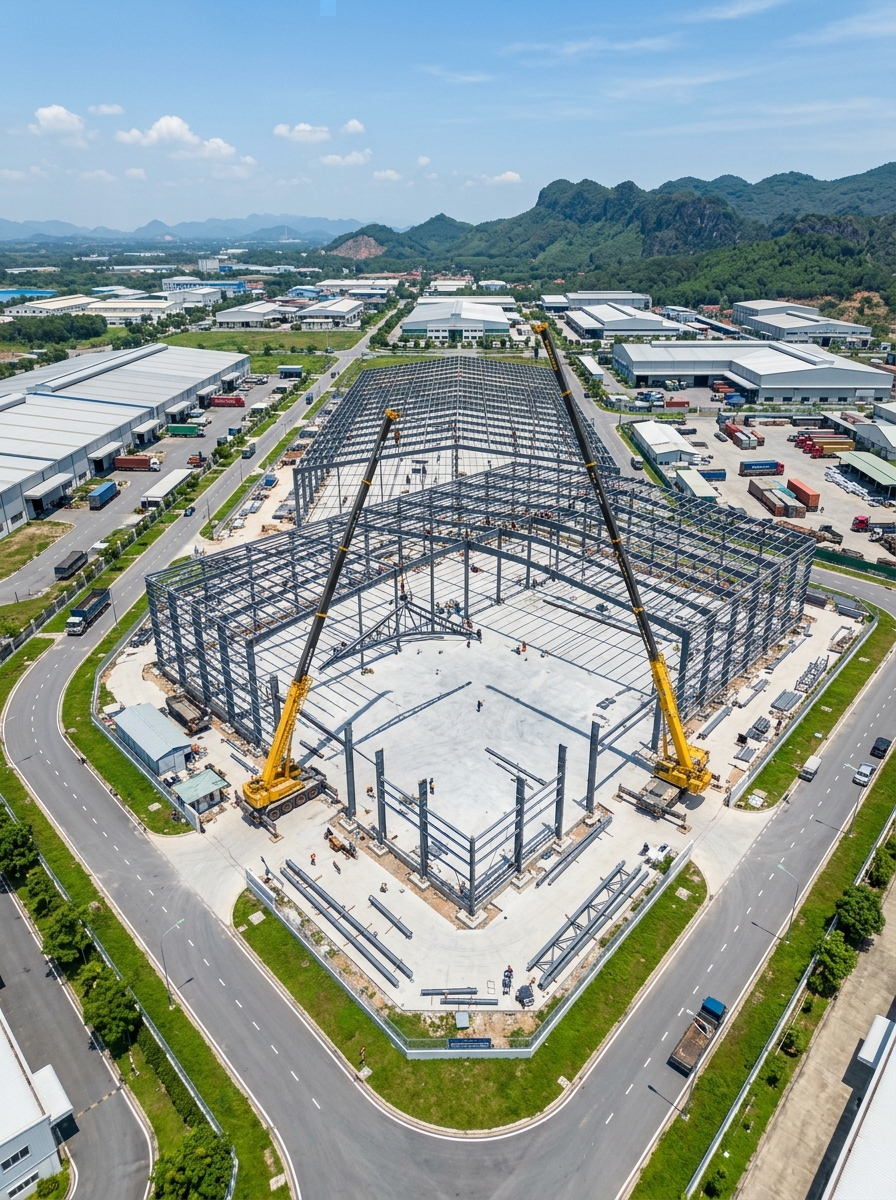
\includegraphics[height=\paperheight]{../../public/executive-cover-hero.jpg}
  };

  % 2. A dark-to-clear gradient protects the copy without hiding the construction image.
  \shade[
    left color=TTCDeepNavy!96!black,
    right color=transparent,
    opacity=0.70
  ] (current page.south west) rectangle (current page.north east);

  % 3. TTC recognition bar and compact logo lock-up.
  \fill[TTCRed] (current page.north west) rectangle ++(\paperwidth, -2.2mm);
  \node[anchor=north west, fill=white, fill opacity=0.96, text opacity=1,
        rounded corners=1.5pt, inner xsep=5mm, inner ysep=3.8mm]
    at ([xshift=15mm,yshift=-13mm]current page.north west) {
      
\includegraphics[width=48mm]{../../public/logo-ttc-removebg-DNXrVdJp.png}
    };
  \node[anchor=north east, text=white, inner sep=0pt] at ([xshift=-15mm,yshift=-15mm]current page.north east) {
    {\fontsize{8}{10}\selectfont\bfseries COMPANY PROFILE \;|\; 2026}
  };

  % 4. Large left-aligned title fills the visual centre; the clear right side shows the site.
  \node[anchor=west, align=left, text width=128mm, inner sep=0pt]
    at ([xshift=16mm,yshift=160mm]current page.south west) {
      {\fontsize{7.8}{9.6}\selectfont\bfseries\color{TTCRed} TAN THANH CONG TECHNOLOGY CONSTRUCTION JOINT STOCK COMPANY}\\[6mm]
      {\fontsize{43}{49}\selectfont\bfseries\color{white} COMPANY}\\[-2mm]
      {\fontsize{43}{49}\selectfont\bfseries\color{white} PROFILE}\\[4mm]
      {\color{TTCRed}\rule{73mm}{2.8pt}}\\[5mm]
      {\fontsize{17}{20}\selectfont\bfseries\color{white} COMPANY PROFILE}\\[10mm]
      {\fontsize{14}{17}\selectfont\bfseries\color{white} INDUSTRIAL GENERAL CONTRACTOR\\INTEGRATED}\\[3mm]
      {\fontsize{9.5}{12}\selectfont\color{white!88!gray} Integrated Industrial Design, Build \& Delivery}
    };

  % 5. Proof points: compact, scannable and placed above the contact footer.
  \node[anchor=south west, align=left, fill=TTCDeepNavy!92!black, fill opacity=0.84,
        text=white, text opacity=1, rounded corners=1.5pt, inner xsep=6mm, inner ysep=4mm]
    at ([xshift=15mm,yshift=31mm]current page.south west) {
      {\fontsize{11}{13}\selectfont\bfseries INDUSTRIAL GENERAL CONTRACTOR \qquad GRADE II CONSTRUCTION CAPABILITY \qquad ISO MANAGEMENT SYSTEMS}\\[1.2mm]
      {\fontsize{7}{8.5}\selectfont\color{white!82!gray}Design, construction capacity and handover industrial works}
    };

  % 6. Legal identity stays quiet; the cover remains a visual statement.
  \node[anchor=south west, text=white, inner sep=0pt] at ([xshift=15mm,yshift=19mm]current page.south west) {
    {\fontsize{6.6}{8.2}\selectfont\bfseries TAN THANH CONG TECHNOLOGY CONSTRUCTION JOINT STOCK COMPANY}
  };

  % 7. Persistent contact footer.
  \fill[TTCDeepNavy!97!black] (current page.south west) rectangle ++(\paperwidth, 11mm);
  \fill[TTCRed] ([yshift=11mm]current page.south west) rectangle ++(\paperwidth, 1.2mm);
  \node[anchor=south, text=white, inner sep=0pt] at ([yshift=3.4mm]current page.south) {
    {\fontsize{6.8}{8.2}\selectfont
      \faPhone\ +84 976 447 766 \quad\textbullet\quad
      \faEnvelope\ info@tanthanhcongjsc.com \quad\textbullet\quad
      \faGlobe\ tanthanhcongjsc.com \quad\textbullet\quad
      \faAward\ CERTIFICATE GRADE II CONSTRUCTION CAPABILITY}
  };
\end{tikzpicture}
\mbox{}% Anchor the overlay to a physical page before advancing to page 02.
\newpage

% ============================================================
% PAGE 02: MỤC LỤC ĐIỀU HƯỚNG & THÔNG TIN PHÁP NHÂN TÓM TẮT
% ============================================================
\pageheaderbar{CONTENTS \& CORPORATE INFORMATION}{Page 02}
\pagefooterbar{Page 02}

\begin{tikzpicture}[remember picture, overlay]
  \node[opacity=0.025, scale=4.2, font=\bfseries\sffamily, text=TTCBlue]
    at ([xshift=30mm,yshift=-8mm]current page.center) {TTC};
  \fill[TTCRed, opacity=0.05] ([xshift=12mm,yshift=18mm]current page.south west)
    rectangle ([xshift=18mm,yshift=248mm]current page.south west);
\end{tikzpicture}

\begin{minipage}[t][246mm]{\textwidth}
\secbrand{Executive Contents}{Executive Contents — 06 Focus Categories}

{\fontsize{9.2}{11.5}\selectfont\color{TTCTextMuted}
The dossier is organized in 06 capacity groups for Client to quickly look up; details of each item are presented on the thematic pages.}\\[3mm]

% Navigation cards: inspired by section-based contents, without repeating every page title.
\newcommand{\toccard}[5]{%
  \begin{tikzpicture}
    \node[rounded corners=3pt, fill=white, draw=TTCBorder, line width=0.8pt,
          minimum width=90mm, minimum height=52mm, text width=79mm, inner sep=5.5mm, align=left] {
      {\fontsize{18}{19}\selectfont\bfseries\color{TTCRed} #1}\hspace{3mm}
      {\fontsize{8.2}{9.5}\selectfont\bfseries\color{TTCRed} PAGE #2}\\[1.5mm]
      {\fontsize{11.2}{13.2}\selectfont\bfseries\color{TTCBlue} #3}\\[0.3mm]
      {\fontsize{7.2}{8.8}\selectfont\itshape\color{TTCTextMuted} #4}\\[3mm]
      {\fontsize{8.2}{10.5}\selectfont\color{TTCTextDark} #5}
    };
  \end{tikzpicture}%
}

\noindent
\begin{tabular}{@{}p{91mm}@{\hspace{4mm}}p{91mm}@{}}
\toccard{I}{01--07}{INTRODUCTION \& PROFILE}{Company profile \& credentials}{Open letter \textbullet\ Vision and Values \textbullet\ Ecosystem \textbullet\ Legal Entity \& leadership} &
\toccard{IV}{14--19}{SOLUTIONS \& TECHNOLOGY}{Integrated delivery \& technology}{Design--integrated labor \textbullet\ Building information model \textbullet\ quality \textbullet\ safety} \\[3.5mm]
\toccard{II}{08--10}{GOVERNANCE \& RESOURCES}{Governance \& people}{Expense Management \textbullet\ guaranteed capacity \textbullet\ resource mobilization \textbullet\ safety culture} &
\toccard{V}{20--30}{Project \& CUSTOMER}{Projects \& valued partners}{Project Category \textbullet\ 06 project documents \textbullet\ supply chain \textbullet\ international partners} \\[3.5mm]
\toccard{III}{11--13}{MANUFACTURING \& GOVERNANCE}{Fabrication \& project control}{Production partners \textbullet\ motorized equipment \textbullet\ contract administration process} &
\toccard{VI}{31--36}{COMMITMENT \& COMPANION}{Commitments \& support}{Certification \textbullet\ Construction coverage \textbullet\ Strategy \textbullet\ Warranty \& contact}
\end{tabular}

\vspace{4.5mm}

% Compact legal snapshot: details remain on the legal-credentials spread (page 06).
\noindent
\begin{tikzpicture}
  \node[rounded corners=3pt, fill=TTCLightBlue, draw=TTCBorder, line width=0.8pt,
        minimum width=186mm, text width=172mm, inner sep=7mm] {
    {\fontsize{10.5}{12.5}\selectfont\bfseries\color{TTCBlue} \faIdCard\quad COMPANY SUMMARY LEGAL ENTITY}
    \hfill {\fontsize{7.2}{8.8}\selectfont\color{TTCRed}\bfseries CERTIFICATE DETAILS: PAGE 06}\\[1.5mm]
    {\fontsize{6.2}{7.5}\selectfont\color{TTCTextMuted}\bfseries
    TAN THANH CONG TECHNOLOGY CONSTRUCTION JOINT STOCK COMPANY}\\[3mm]
    \renewcommand{\arraystretch}{1.28}
    {\fontsize{8.2}{10.2}\selectfont
    \begin{tabularx}{\linewidth}{@{}p{32mm}X@{\hspace{5mm}}p{28mm}X@{}}
      \textbf{Business name} & \textbf{TAN THANH CONG TECHNOLOGY CONSTRUCTION JOINT STOCK COMPANY} &
      \textbf{Tax Identification Number} & \textbf{0107090447} \\
      \textbf{Legal representative} & \textbf{Mr. PHAM HUY TAN} — Chief Executive Officer &
      \textbf{Competencies} & Construction capacity certificate Class II \textbullet\ ISO Management System \\
      \textbf{Registered office} & No. 39, Lane 292 Kim Giang, Dai Kim, Hanoi &
      \textbf{Transaction office} & No. 19N7B, Urban area Trung Hoa Nhan Chinh, Hanoi \\
      \textbf{Contact} & +84 976 447 766 \textbullet\ info@tanthanhcongjsc.com &
      \textbf{Website} & tanthanhcongjsc.com
    \end{tabularx}}\\[2mm]
    {\fontsize{5.5}{6.8}\selectfont\color{TTCTextMuted}
    \textbf{Key Terminology:} EPC -- Design, Procurement and Construction; PEB -- Pre-engineered Steel Building; MEP -- M\&E; BIM -- Building Information Modeling;\\[-0.3mm]
    QA/QC -- Assurance and Control of quality; HSE -- Safety, Health and Environment; Fire Protection -- Fire Prevention \& Fighting; ITP -- Inspection and Acceptance Plan.}
  };
\end{tikzpicture}
\end{minipage}
\newpage

% ============================================================
% PAGE 03: THÔNG ĐIỆP TỪ TỔNG GIÁM ĐỐC — LEADERSHIP MESSAGE
% ============================================================
\pageheaderbar{MESSAGE FROM THE CEO}{Page 03}
\pagefooterbar{Page 03}

\begin{tikzpicture}[remember picture, overlay]
  \node[opacity=0.025, scale=4.0, font=\bfseries\sffamily, text=TTCBlue]
    at ([xshift=-25mm,yshift=-25mm]current page.center) {LEADERSHIP};
  \fill[TTCRed, opacity=0.045] ([xshift=12mm,yshift=18mm]current page.south west)
    rectangle ([xshift=18mm,yshift=248mm]current page.south west);
\end{tikzpicture}

\begin{minipage}[t][246mm]{\textwidth}
\secbrand{Message from the CEO}{Leadership Message — Building Trust Through Every Commitment}

\vspace{2mm}

% Main editorial spread: concise letter on the left, authentic CEO portrait on the right.
\noindent
\begin{tabular}{@{}p{106mm}@{\hspace{4mm}}p{76mm}@{}}
  
\begin{tikzpicture}
    \path[use as bounding box] (0,0) rectangle (106mm,170mm);
    \draw[TTCRed, line width=2.2pt] (0,169mm) -- (26mm,169mm);
    \node[anchor=north west, align=left, text width=98mm, inner sep=0pt] at (0,165mm) {
      {\fontsize{8.5}{10}\selectfont\bfseries\color{TTCRed} TTC'S ENDURING MESSAGE}\\[4mm]
      {\fontsize{19}{23}\selectfont\bfseries\color{TTCBlue}
      ``QUALITY IS OUR HONOUR.\\
      SAFETY IS OUR LIFELINE.\\
      WE DELIVER AS PROMISED.''}\\[6mm]
      {\fontsize{10}{12}\selectfont\bfseries\color{TTCBlue}
      Dear Clients and Partners,}\\[3mm]
      {\fontsize{9.2}{13.2}\selectfont\color{TTCTextDark}
      On behalf of the Board of Directors and all employees of \textbf{Tan Thanh Cong Technology Construction Joint Stock Company}, I sincerely thank you for your trust and partnership throughout TTC's development journey.\\[3mm]

      More than a decade in industrial construction has taught us that every successful project must achieve \textbf{quality, safety, schedule and investment efficiency}. Tan Thanh Cong therefore operates through \textbf{a single point of responsibility for design--procurement--construction}, supported by value engineering, building information modelling and disciplined site management.\\[3mm]

      Through our steel-fabrication partner network and experienced field engineers, we provide fit-for-purpose solutions with transparent control from design and construction through handover and warranty.\\[3mm]

      TTC aims to be more than a contractor: a \textbf{long-term value-creation partner} for every client and every project.}\\[5mm]
      {\fontsize{9}{11}\selectfont\itshape\color{TTCTextMuted} Sincerely,}
    };
  \end{tikzpicture}
  &
  \begin{tikzpicture}
    \path[use as bounding box] (0,0) rectangle (76mm,170mm);
    \fill[TTCLightBlue] (0,0) rectangle (76mm,170mm);
    \draw[TTCBorder, line width=0.8pt] (0,0) rectangle (76mm,170mm);
    \fill[TTCRed] (0,0) rectangle (3mm,170mm);

    \node[anchor=north, inner sep=0pt] at (39.5mm,168mm) {
      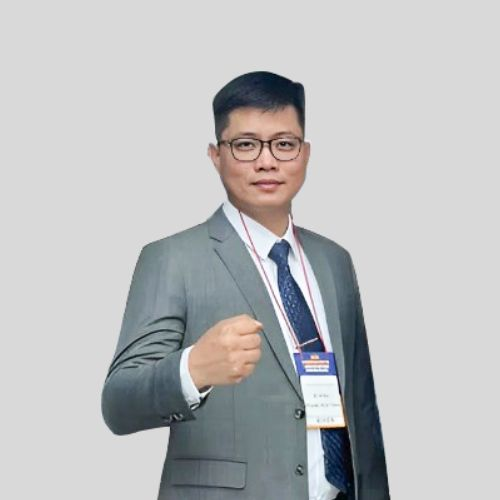
\includegraphics[trim=90 0 90 0,clip,height=116mm]{../tan_avatar.jpg}
    };

    \fill[TTCDeepNavy!97!black] (3mm,0) rectangle (76mm,54mm);
    \fill[TTCRed] (3mm,54mm) rectangle (76mm,56mm);
    \node[anchor=north west, align=left, text width=62mm, inner sep=0pt]
      at (10mm,46mm) {
        {\fontsize{7}{8.5}\selectfont\bfseries\color{TTCRed} CHIEF EXECUTIVE OFFICER / CEO}\\[2mm]
        {\fontsize{14}{17}\selectfont\bfseries\color{white} PHAM HUY TAN}\\[2mm]
        {\fontsize{7.5}{9.5}\selectfont\color{white!78!gray}
        Technology Joint Stock Company\\Construction of Tan Thanh Cong}\\[4mm]
        {\fontsize{7.2}{9}\selectfont\bfseries\color{white!68!gray} TAN THANH CONG \textbullet\ TTC JSC}
      };
  \end{tikzpicture}
\end{tabular}

\vspace{5mm}

% Three commitments replace the duplicated vision/mission content.
\noindent
\begin{tabular}{@{}p{58mm}@{\hspace{6mm}}p{58mm}@{\hspace{6mm}}p{58mm}@{}}
  \begin{tikzpicture}
    \node[rounded corners=3pt, fill=TTCDeepNavy!97!black, minimum width=58mm,
          minimum height=43mm, text width=48mm, align=center, inner sep=5mm] {
      {\fontsize{17}{19}\selectfont\bfseries\color{white} 01}\\[1mm]
      {\fontsize{9}{11}\selectfont\bfseries\color{TTCRed} ONE CONTRACT}\\[2mm]
      {\fontsize{7.3}{9}\selectfont\color{white!78!gray}Design \textbullet\ Build \textbullet\ Handover}
    };
  \end{tikzpicture}
  &
  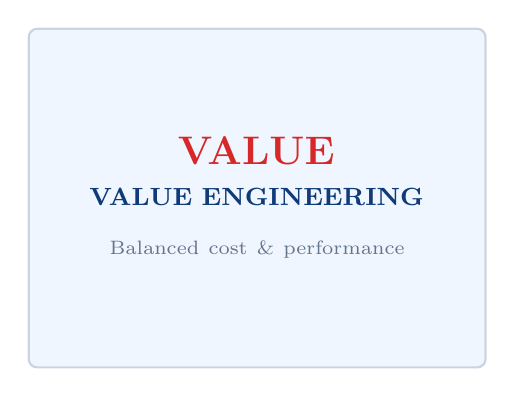
\begin{tikzpicture}
    \node[rounded corners=3pt, fill=TTCLightBlue, draw=TTCBorder, line width=0.8pt,
          minimum width=58mm, minimum height=43mm, text width=48mm, align=center, inner sep=5mm] {
      {\fontsize{15}{18}\selectfont\bfseries\color{TTCRed} VALUE}\\[1mm]
      {\fontsize{9}{11}\selectfont\bfseries\color{TTCBlue} VALUE ENGINEERING}\\[2mm]
      {\fontsize{7.3}{9}\selectfont\color{TTCTextMuted}Balanced cost \& performance}
    };
  \end{tikzpicture}
  &
  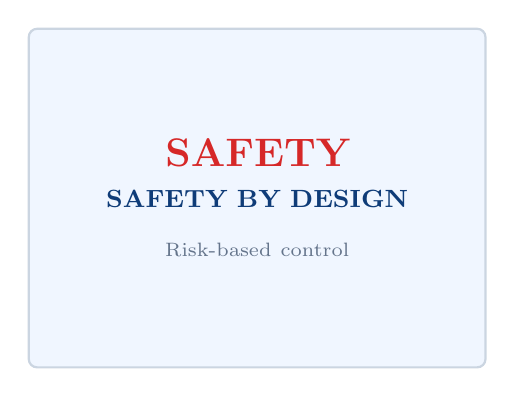
\begin{tikzpicture}
    \node[rounded corners=3pt, fill=TTCLightBlue, draw=TTCBorder, line width=0.8pt,
          minimum width=58mm, minimum height=43mm, text width=48mm, align=center, inner sep=5mm] {
      {\fontsize{15}{18}\selectfont\bfseries\color{TTCRed} SAFETY}\\[1mm]
      {\fontsize{9}{11}\selectfont\bfseries\color{TTCBlue} SAFETY BY DESIGN}\\[2mm]
      {\fontsize{7.3}{9}\selectfont\color{TTCTextMuted}Risk-based control}
    };
  \end{tikzpicture}
\end{tabular}

\vspace{6mm}

\noindent
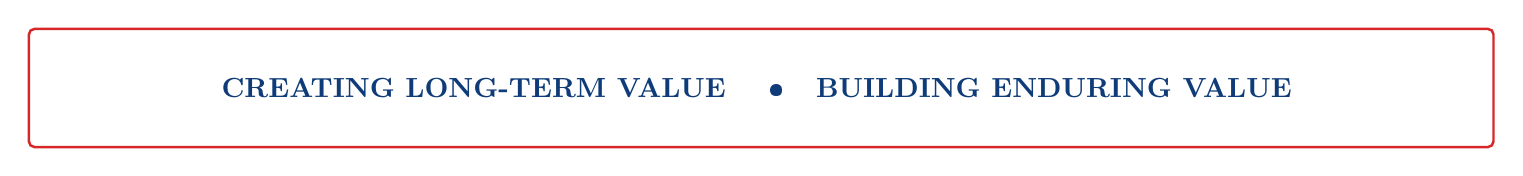
\begin{tikzpicture}
  \node[rounded corners=2pt, fill=white, draw=TTCRed, line width=0.9pt,
        minimum width=186mm, minimum height=15mm, align=center, inner sep=3mm] {
    {\fontsize{10}{12}\selectfont\bfseries\color{TTCBlue}
    CREATING LONG-TERM VALUE \quad\textbullet\quad BUILDING ENDURING VALUE}
  };
\end{tikzpicture}
\end{minipage}
\newpage

% ============================================================
% PAGE 04: KẾT CẤU VƯƠN CAO — HÀNH TRÌNH & GIÁ TRỊ CỐT LÕI
% ============================================================
\pageheaderbar{DEVELOPMENT JOURNEY \& CORE VALUES}{Page 04}
\pagefooterbar{Page 04}

\begin{tikzpicture}[remember picture, overlay]
  \node[opacity=0.022, scale=4.0, font=\bfseries\sffamily, text=TTCBlue]
    at ([xshift=15mm,yshift=-18mm]current page.center) {BUILDING THE FUTURE};
\end{tikzpicture}

\begin{minipage}[t][246mm]{\textwidth}
\secbrand{Our Development Journey}{From Mechanical Foundations to a Next-Generation EPC General Contractor}

\vspace{1mm}

\noindent

\begin{tikzpicture}
  \node[anchor=west, align=left, inner sep=0pt] at (0,7mm) {
    {\fontsize{16}{19}\selectfont\bfseries\color{TTCBlue}
    FROM MECHANICAL FOUNDATIONS TO NEXT-GENERATION EPC}\\[1.5mm]
    {\fontsize{7.8}{9.5}\selectfont\color{TTCTextMuted}
    A development journey built on delivery capability, technology and enduring values.}
  };
  \fill[TTCRed] (0,0) rectangle (52mm,1.4mm);
\end{tikzpicture}

\vspace{3mm}

% Diagonal growth spine — a steel-beam metaphor for TTC's development.
\noindent
\begin{tikzpicture}[x=1mm,y=1mm]
  \path[use as bounding box] (0,0) rectangle (186,112);
  \fill[TTCLightBlue!55!white] (0,0) rectangle (186,112);
  \draw[TTCBorder, line width=0.8pt, rounded corners=3pt] (0,0) rectangle (186,112);
  \draw[TTCBlue!7!white, line width=0.35pt] (0,0) grid[step=10mm] (186,112);

  % Stepped structural spine: horizontal floor plates linked by rising steel members.
  \draw[TTCBlue!10!white, line width=7pt, line join=round]
    (16,19) -- (44,19) -- (52,40) -- (76,40) -- (84,61) --
    (116,61) -- (124,82) -- (155,82) -- (163,105) -- (180,105);
  \draw[TTCBlue!28!white, line width=1pt, line join=round]
    (12,14) -- (41,14) -- (49,35) -- (73,35) -- (81,56) --
    (113,56) -- (121,77) -- (152,77) -- (160,100) -- (177,100);
  \draw[TTCRed, line width=3.2pt, line join=round]
    (16,19) -- (44,19) -- (52,40) -- (76,40) -- (84,61) --
    (116,61) -- (124,82) -- (155,82) -- (163,105) -- (180,105);
  \draw[TTCRed, line width=1.1pt, -{Stealth[length=4mm]}] (180,105) -- (184,109);

  % 2015
  \fill[white] (16,19) circle (3.4);
  \draw[TTCRed, line width=1.5pt] (16,19) circle (3.4);
  \fill[TTCRed] (16,19) circle (1.35);
  \node[anchor=south west, align=left, text width=38mm, fill=TTCLightBlue!86!white,
        fill opacity=0.94, text opacity=1, rounded corners=1.5pt, inner sep=1mm] at (7,25) {
    {\fontsize{18}{20}\selectfont\bfseries\color{TTCRed} 2015}\\[-0.5mm]
    {\fontsize{8.5}{10}\selectfont\bfseries\color{TTCBlue} FOUNDATION}\\[1mm]
    {\fontsize{7.2}{9}\selectfont\color{TTCTextDark}Precision Mechanical Platform\\and steel structure technique.}
  };

  % 2018
  \fill[white] (55,40) circle (3.4);
  \draw[TTCRed, line width=1.5pt] (55,40) circle (3.4);
  \fill[TTCRed] (55,40) circle (1.35);
  \node[anchor=north west, align=left, text width=38mm, fill=TTCLightBlue!86!white,
        fill opacity=0.94, text opacity=1, rounded corners=1.5pt, inner sep=1mm] at (38,29) {
    {\fontsize{18}{20}\selectfont\bfseries\color{TTCRed} 2018}\\[-0.5mm]
    {\fontsize{8.5}{10}\selectfont\bfseries\color{TTCBlue} EXPAND}\\[1mm]
    {\fontsize{7.2}{9}\selectfont\color{TTCTextDark}PEB production links\\and industrial infrastructure delivery.}
  };

  % 2022
  \fill[white] (94,61) circle (3.4);
  \draw[TTCRed, line width=1.5pt] (94,61) circle (3.4);
  \fill[TTCRed] (94,61) circle (1.35);
  \node[anchor=south west, align=left, text width=39mm, fill=TTCLightBlue!86!white,
        fill opacity=0.94, text opacity=1, rounded corners=1.5pt, inner sep=1mm] at (71,67) {
    {\fontsize{18}{20}\selectfont\bfseries\color{TTCRed} 2022}\\[-0.5mm]
    {\fontsize{8.5}{10}\selectfont\bfseries\color{TTCBlue} BREAKTHROUGH}\\[1mm]
    {\fontsize{7.2}{9}\selectfont\color{TTCTextDark}Construction capability certification\\and multidisciplinary industrial project.}
  };

  % 2026
  \fill[white] (134,82) circle (3.4);
  \draw[TTCRed, line width=1.5pt] (134,82) circle (3.4);
  \fill[TTCRed] (134,82) circle (1.35);
  \node[anchor=north west, align=left, text width=42mm, fill=TTCLightBlue!86!white,
        fill opacity=0.94, text opacity=1, rounded corners=1.5pt, inner sep=1mm] at (119,68) {
    {\fontsize{18}{20}\selectfont\bfseries\color{TTCRed} 2026}\\[-0.5mm]
    {\fontsize{8.5}{10}\selectfont\bfseries\color{TTCBlue} TRANSFORM}\\[1mm]
    {\fontsize{7.2}{9}\selectfont\color{TTCTextDark}Standardized project management\\and project data systems.}
  };

  % 2030
  \fill[white] (176,105) circle (3.4);
  \draw[TTCRed, line width=1.5pt] (176,105) circle (3.4);
  \fill[TTCRed] (176,105) circle (1.35);
  \node[anchor=north east, align=right, text width=40mm, fill=TTCLightBlue!86!white,
        fill opacity=0.94, text opacity=1, rounded corners=1.5pt, inner sep=1mm] at (178,98) {
    {\fontsize{18}{20}\selectfont\bfseries\color{TTCRed} 2030}\\[-0.5mm]
    {\fontsize{8.5}{10}\selectfont\bfseries\color{TTCBlue} REGIONAL GROWTH}\\[1mm]
    {\fontsize{7.2}{9}\selectfont\color{TTCTextDark}ConTech \textbullet\ ESG\\Expanding Southeast Asia.}
  };
\end{tikzpicture}

\vspace{4mm}

% Photo foundation: five core values become the structural base of the journey.
\noindent
\begin{tikzpicture}[x=1mm,y=1mm]
  \path[use as bounding box] (0,0) rectangle (186,112);
  \clip[rounded corners=3pt] (0,0) rectangle (186,112);
  \node[anchor=center, inner sep=0pt] at (93,56) {
    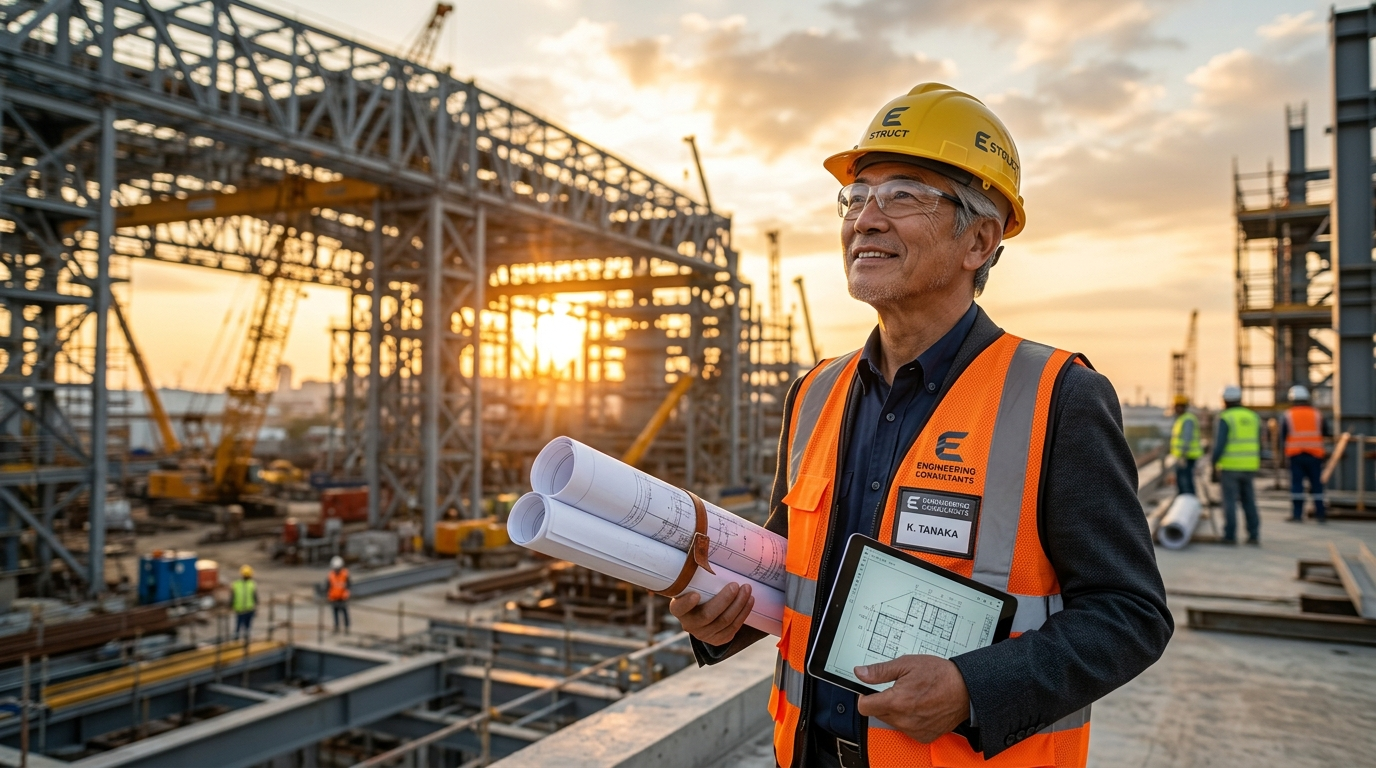
\includegraphics[height=112mm]{../05-company-profile/assets/milestones_engineer_hero.jpg}
  };
  \shade[left color=TTCDeepNavy!98!black, right color=transparent, opacity=0.82]
    (0,31) rectangle (142,112);
  \node[anchor=north west, align=left, text width=112mm, inner sep=0pt] at (8,104) {
    {\fontsize{12}{14}\selectfont\bfseries\color{white}FIVE VALUES — THE FOUNDATION OF EVERY PROJECT}\\[1.5mm]
    {\fontsize{7.5}{9}\selectfont\color{white!82!gray}The values that sustain every commitment and every project.}
  };

  \fill[TTCDeepNavy!97!black, opacity=0.96] (0,0) rectangle (37.2,31);
  \fill[TTCDeepNavy!91!black, opacity=0.96] (37.2,0) rectangle (74.4,31);
  \fill[TTCDeepNavy!97!black, opacity=0.96] (74.4,0) rectangle (111.6,31);
  \fill[TTCDeepNavy!91!black, opacity=0.96] (111.6,0) rectangle (148.8,31);
  \fill[TTCDeepNavy!97!black, opacity=0.96] (148.8,0) rectangle (186,31);
  \fill[TTCRed] (0,31) rectangle (186,32.3);

  \node[align=center, text=white] at (18.6,15.5) {
    {\fontsize{14}{16}\selectfont\bfseries TRUST}\\[1mm]
    {\fontsize{6.8}{8}\selectfont\color{white!72!gray}TRUST \& INTEGRITY}
  };
  \node[align=center, text=white] at (55.8,15.5) {
    {\fontsize{14}{16}\selectfont\bfseries DEDICATION}\\[1mm]
    {\fontsize{6.8}{8}\selectfont\color{white!72!gray}DEDICATION}
  };
  \node[align=center, text=white] at (93,15.5) {
    {\fontsize{14}{16}\selectfont\bfseries MIND}\\[1mm]
    {\fontsize{6.8}{8}\selectfont\color{white!72!gray}INNOVATION}
  };
  \node[align=center, text=white] at (130.2,15.5) {
    {\fontsize{14}{16}\selectfont\bfseries SPEED}\\[1mm]
    {\fontsize{6.8}{8}\selectfont\color{white!72!gray}FAST-TRACK}
  };
  \node[align=center, text=white] at (167.4,15.5) {
    {\fontsize{14}{16}\selectfont\bfseries SAFETY}\\[1mm]
    {\fontsize{6.8}{8}\selectfont\color{white!72!gray}HSE \& SAFETY}
  };
\end{tikzpicture}
\end{minipage}
\newpage

% ============================================================
% PAGE 05: INTEGRATED FACTORY BLUEPRINT
% ============================================================
\pageheaderbar{DESIGN ECOSYSTEM \& CONSTRUCTION OF INTEGRATED}{Page 05}
\pagefooterbar{Page 05}

\begin{tikzpicture}[remember picture, overlay]
  \draw[TTCBlue!6!white, line width=0.45pt]
    ([xshift=15mm,yshift=18mm]current page.south west)
    grid[step=8mm]
    ([xshift=195mm,yshift=42mm]current page.south west);
\end{tikzpicture}

\begin{minipage}[t][246mm]{\textwidth}
\secbrand{Design Ecosystem \& Integrated Construction}{Integrated Factory Blueprint \& AIDC ConTech Collaboration}

\vspace{1mm}
{\fontsize{15}{17}\selectfont\bfseries\color{TTCBlue}
ONE ECOSYSTEM • ONE CONTRACT • ONE RESPONSIBILITY\par}
\vspace{1mm}
{\fontsize{7.5}{9}\selectfont\color{TTCTextMuted}
One integrated ecosystem. One accountable EPC partner from concept to handover.\par}
\vspace{3mm}

% HERO: NHÀ MÁY LÀ TRUNG TÂM, NĂNG LỰC LÀ CÁC LỚP TÍCH HỢP
\noindent
\begin{tikzpicture}[x=1mm,y=1mm]
  \path[use as bounding box] (0,0) rectangle (186,118);
  \clip[rounded corners=3pt] (0,0) rectangle (186,118);
  \node[anchor=center, inner sep=0pt] at (93,59)
    {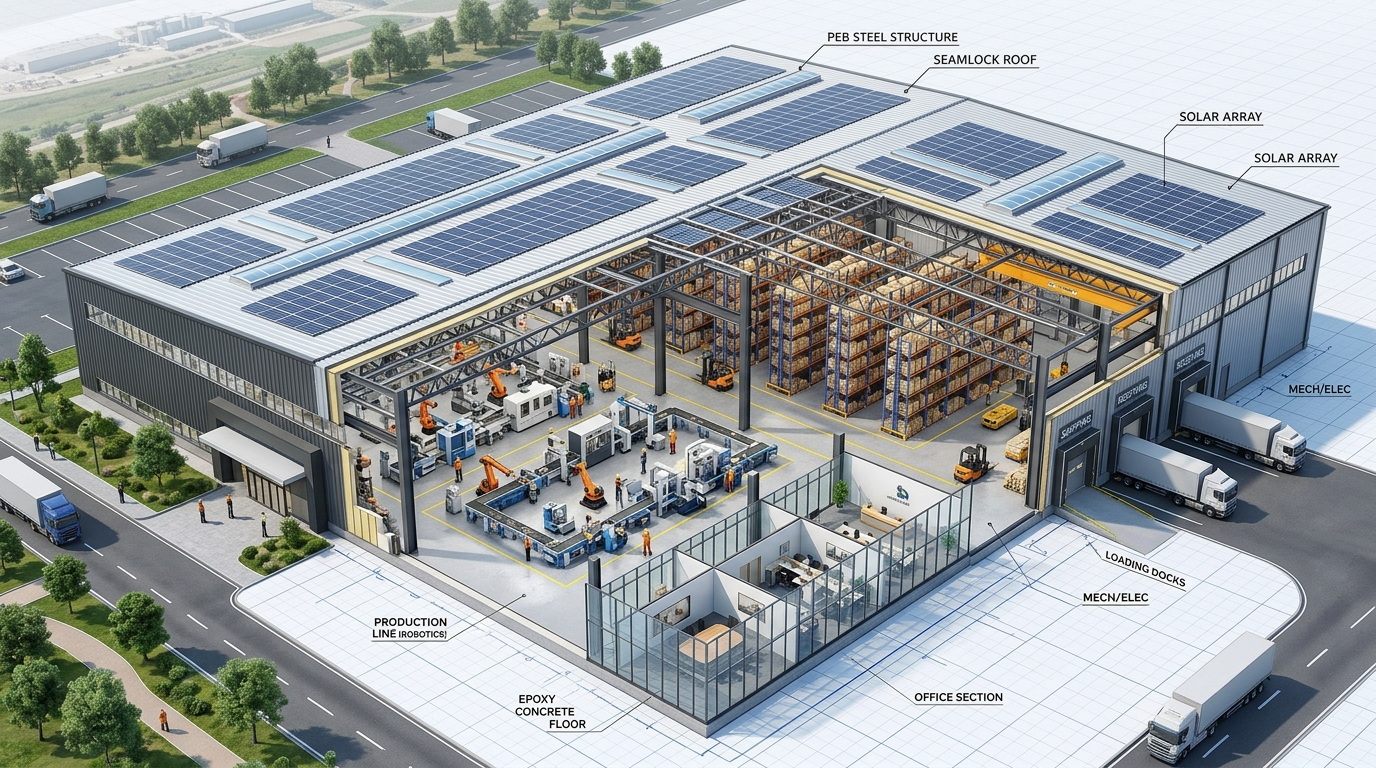
\includegraphics[height=118mm]{../../public/factory-tech-3d.jpg}};
  \fill[white, opacity=0.10] (0,0) rectangle (186,118);

  % Connectors — thin and quiet
  \draw[TTCBlue!55!white, line width=0.65pt] (55,91) -- (80,72);
  \draw[TTCBlue!55!white, line width=0.65pt] (55,38) -- (81,57);
  \draw[TTCBlue!55!white, line width=0.65pt] (131,91) -- (107,72);
  \draw[TTCRed!72!white, line width=0.75pt] (131,38) -- (106,57);

  % 01 — AIDC ConTech
  \node[
    anchor=north west, rounded corners=3pt,
    fill=white, fill opacity=0.94, text opacity=1,
    draw=TTCCyan!70!white, line width=0.65pt,
    minimum width=53mm, minimum height=29mm,
    text width=47mm, inner sep=3mm, align=left
  ] at (5,113) {
    {\fontsize{7.3}{8.5}\selectfont\bfseries\color{TTCCyan} 01 / AIDC CONTECH}\\[1mm]
    {\fontsize{10}{11.5}\selectfont\bfseries\color{TTCBlue} DATA MODEL • VALUE ENGINEERING}\\[1mm]
    {\fontsize{7}{8.6}\selectfont\color{TTCTextDark}Optimize handover design solution, construction capability and data.}
  };

  % 02 — MEP & PCCC
  \node[
    anchor=south west, rounded corners=3pt,
    fill=white, fill opacity=0.94, text opacity=1,
    draw=TTCBlue!42!white, line width=0.65pt,
    minimum width=53mm, minimum height=29mm,
    text width=47mm, inner sep=3mm, align=left
  ] at (5,5) {
    {\fontsize{7.3}{8.5}\selectfont\bfseries\color{TTCBlue} 02 / M\&E \& FIRE PREVENTION}\\[1mm]
    {\fontsize{10}{11.5}\selectfont\bfseries\color{TTCBlue} MODEL-BASED COORDINATION SYSTEM}\\[1mm]
    {\fontsize{7}{8.6}\selectfont\color{TTCTextDark}Electricity • ventilation and air conditioning • water supply and drainage • fire prevention \& fighting.}
  };

  % 03 — Hạ tầng
  \node[
    anchor=north east, rounded corners=3pt,
    fill=white, fill opacity=0.94, text opacity=1,
    draw=TTCBlue!42!white, line width=0.65pt,
    minimum width=53mm, minimum height=29mm,
    text width=47mm, inner sep=3mm, align=left
  ] at (181,113) {
    {\fontsize{7.3}{8.5}\selectfont\bfseries\color{TTCBlue} 03 /INFRASTRUCTURE OF INDUSTRIAL ZONE}\\[1mm]
    {\fontsize{10}{11.5}\selectfont\bfseries\color{TTCBlue} FOUNDATION • ROAD • DRAINAGE}\\[1mm]
    {\fontsize{7}{8.6}\selectfont\color{TTCTextDark}Technical infrastructure is ready for operation, synchronously connected to the total plant site.}
  };

  % 04 — PEB LAST
  \node[
    anchor=south east, rounded corners=3pt,
    fill=white, fill opacity=0.96, text opacity=1,
    draw=TTCRed!78!white, line width=0.8pt,
    minimum width=53mm, minimum height=29mm,
    text width=47mm, inner sep=3mm, align=left
  ] at (181,5) {
    {\fontsize{7.3}{8.5}\selectfont\bfseries\color{TTCRed} 04 / STEEL FABRICATION}\\[1mm]
    {\fontsize{10}{11.5}\selectfont\bfseries\color{TTCBlue} PRODUCTION OF STEEL STRUCTURES}\\[1mm]
    {\fontsize{7}{8.6}\selectfont\color{TTCTextDark}CNC machining • automatic welding • nondestructive testing; mobilization according to project plan.}
  };

  % Central accountability hub
  \node[
    rounded corners=3pt, fill=TTCDeepNavy!96!black,
    draw=TTCCyan!75!white, line width=0.9pt,
    minimum width=50mm, minimum height=28mm,
    text=white, align=center, inner sep=2.5mm
  ] at (93,64) {
    {\fontsize{11}{12.5}\selectfont\bfseries TAN THANH CONG}\\[1mm]
    {\fontsize{7.5}{9}\selectfont\bfseries\color{TTCCyan} EPC SYSTEM INTEGRATOR}\\[1mm]
    {\fontsize{6.8}{8}\selectfont\color{white!78!gray}One contract • One accountability}
  };

  \draw[white, line width=1.2pt, rounded corners=3pt] (0.6,0.6) rectangle (185.4,117.4);
  \draw[TTCBorder, line width=0.65pt, rounded corners=3pt] (0,0) rectangle (186,118);
\end{tikzpicture}

\vspace{3mm}

% DELIVERY FLOW — PEB NẰM CUỐI TRONG CHUỖI NĂNG LỰC
\noindent
\begin{tikzpicture}[x=1mm,y=1mm]
  \path[use as bounding box] (0,0) rectangle (186,31);
  \fill[TTCLightBlue, rounded corners=4pt] (0,0) rectangle (186,31);
  \draw[TTCBorder, line width=0.65pt, rounded corners=4pt] (0,0) rectangle (186,31);

  \node[align=center] at (18,15.5) {
    {\fontsize{7}{8}\selectfont\bfseries\color{TTCTextMuted} 01}\\[0.7mm]
    {\fontsize{9.2}{10.5}\selectfont\bfseries\color{TTCBlue} SURVEY}\\[0.7mm]
    {\fontsize{6.6}{8}\selectfont Current status \& requirements}
  };
  \node[align=center] at (55.5,15.5) {
    {\fontsize{7}{8}\selectfont\bfseries\color{TTCTextMuted} 02}\\[0.7mm]
    {\fontsize{9.2}{10.5}\selectfont\bfseries\color{TTCBlue} DESIGN}\\[0.7mm]
    {\fontsize{6.6}{8}\selectfont BIM • AI • VE}
  };
  \node[align=center] at (93,15.5) {
    {\fontsize{7}{8}\selectfont\bfseries\color{TTCTextMuted} 03}\\[0.7mm]
    {\fontsize{9.2}{10.5}\selectfont\bfseries\color{TTCBlue} INFRASTRUCTURE}\\[0.7mm]
    {\fontsize{6.6}{8}\selectfont Foundation • utilities}
  };
  \node[align=center] at (130.5,15.5) {
    {\fontsize{7}{8}\selectfont\bfseries\color{TTCTextMuted} 04}\\[0.7mm]
    {\fontsize{9.2}{10.5}\selectfont\bfseries\color{TTCBlue} MEP \& PCCC}\\[0.7mm]
    {\fontsize{6.6}{8}\selectfont System Integration}
  };
  \node[align=center] at (168,15.5) {
    {\fontsize{7}{8}\selectfont\bfseries\color{TTCRed} 05}\\[0.7mm]
    {\fontsize{9.2}{10.5}\selectfont\bfseries\color{TTCRed} PEB}\\[0.7mm]
    {\fontsize{6.6}{8}\selectfont Manufacturing • erection}
  };

  \foreach \x in {36.75,74.25,111.75,149.25}{
    \node[text=TTCRed, font=\fontsize{8}{9}\selectfont] at (\x,15.5) {\faChevronRight};
  }
\end{tikzpicture}

\vspace{3mm}

% THREE BUSINESS OUTCOMES — LIGHTER THAN THE OLD DARK KPI BAND
\noindent
\begin{tabular}{@{}p{58mm}@{\hspace{6mm}}p{58mm}@{\hspace{6mm}}p{58mm}@{}}
  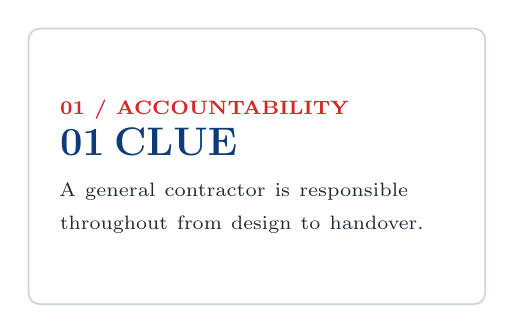
\begin{tikzpicture}
    \node[
      rounded corners=4pt, fill=white, draw=TTCBorder,
      line width=0.65pt, minimum width=58mm, minimum height=35mm,
      text width=50mm, inner sep=4mm, align=left
    ] {
      {\fontsize{7}{8}\selectfont\bfseries\color{TTCRed} 01 / ACCOUNTABILITY}\\[1mm]
      {\fontsize{14}{15.5}\selectfont\bfseries\color{TTCBlue} 01 CLUE}\\[1mm]
      {\fontsize{7}{8.5}\selectfont\color{TTCTextDark}A general contractor is responsible throughout from design to handover.}
    };
  \end{tikzpicture}
  &
  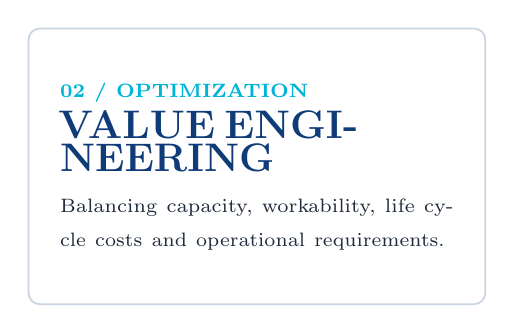
\begin{tikzpicture}
    \node[
      rounded corners=4pt, fill=white, draw=TTCBorder,
      line width=0.65pt, minimum width=58mm, minimum height=35mm,
      text width=50mm, inner sep=4mm, align=left
    ] {
      {\fontsize{7}{8}\selectfont\bfseries\color{TTCCyan} 02 / OPTIMIZATION}\\[1mm]
      {\fontsize{14}{15.5}\selectfont\bfseries\color{TTCBlue} VALUE ENGINEERING}\\[1mm]
      {\fontsize{7}{8.5}\selectfont\color{TTCTextDark}Balancing capacity, workability, life cycle costs and operational requirements.}
    };
  \end{tikzpicture}
  &
  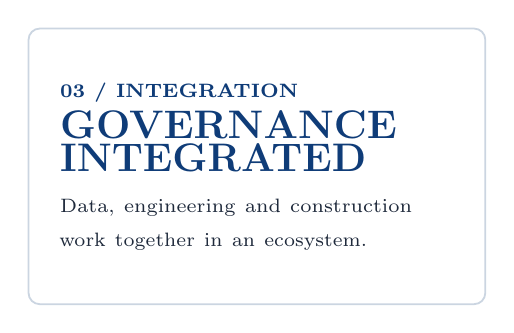
\begin{tikzpicture}
    \node[
      rounded corners=4pt, fill=white, draw=TTCBorder,
      line width=0.65pt, minimum width=58mm, minimum height=35mm,
      text width=50mm, inner sep=4mm, align=left
    ] {
      {\fontsize{7}{8}\selectfont\bfseries\color{TTCBlue} 03 / INTEGRATION}\\[1mm]
      {\fontsize{14}{15.5}\selectfont\bfseries\color{TTCBlue} GOVERNANCE INTEGRATED}\\[1mm]
      {\fontsize{7}{8.5}\selectfont\color{TTCTextDark}Data, engineering and construction work together in an ecosystem.}
    };
  \end{tikzpicture}
\end{tabular}

\vspace{3mm}

% TRUST STRIP — INTERNATIONAL CONTROL STANDARDS
\noindent
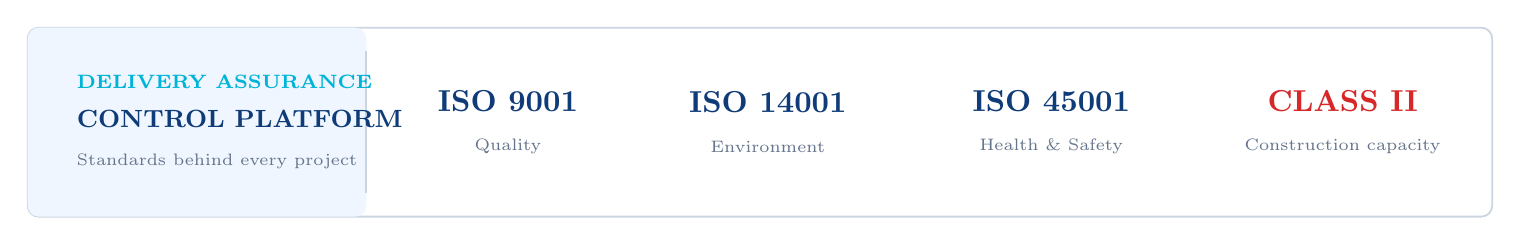
\begin{tikzpicture}[x=1mm,y=1mm]
  \path[use as bounding box] (0,0) rectangle (186,24);
  \fill[white, rounded corners=4pt] (0,0) rectangle (186,24);
  \draw[TTCBorder, line width=0.65pt, rounded corners=4pt] (0,0) rectangle (186,24);
  \fill[TTCLightBlue, rounded corners=4pt] (0,0) rectangle (43,24);
  \draw[TTCBorder, line width=0.55pt] (43,3) -- (43,21);

  \node[anchor=west, align=left] at (5,12) {
    {\fontsize{7}{8}\selectfont\bfseries\color{TTCCyan} DELIVERY ASSURANCE}\\[0.8mm]
    {\fontsize{9}{10.5}\selectfont\bfseries\color{TTCBlue} CONTROL PLATFORM}\\[0.6mm]
    {\fontsize{6.4}{7.8}\selectfont\color{TTCTextMuted} Standards behind every project}
  };
  \node[align=center] at (61,12) {
    {\fontsize{11}{12.5}\selectfont\bfseries\color{TTCBlue} ISO 9001}\\[0.8mm]
    {\fontsize{6.5}{8}\selectfont\color{TTCTextMuted} Quality}
  };
  \node[align=center] at (94,12) {
    {\fontsize{11}{12.5}\selectfont\bfseries\color{TTCBlue} ISO 14001}\\[0.8mm]
    {\fontsize{6.5}{8}\selectfont\color{TTCTextMuted} Environment}
  };
  \node[align=center] at (130,12) {
    {\fontsize{11}{12.5}\selectfont\bfseries\color{TTCBlue} ISO 45001}\\[0.8mm]
    {\fontsize{6.5}{8}\selectfont\color{TTCTextMuted} Health \& Safety}
  };
  \node[align=center] at (167,12) {
    {\fontsize{11}{12.5}\selectfont\bfseries\color{TTCRed} CLASS II}\\[0.8mm]
    {\fontsize{6.5}{8}\selectfont\color{TTCTextMuted} Construction capacity}
  };
\end{tikzpicture}
\end{minipage}
\newpage

% ============================================================
% PAGE 06: GOVERNANCE & COMPLIANCE DASHBOARD
% ============================================================
\pageheaderbar{GOVERNANCE \& CONSTRUCTION CAPABILITY}{Page 06}
\pagefooterbar{Page 06}

\begin{tikzpicture}[remember picture, overlay]
  \draw[TTCBlue!6!white, line width=0.45pt]
    ([xshift=15mm,yshift=18mm]current page.south west)
    grid[step=8mm]
    ([xshift=195mm,yshift=42mm]current page.south west);
\end{tikzpicture}

\begin{minipage}[t][246mm]{\textwidth}
\secbrand{Lean Management \& Compliance Platform}{Governance Structure, Grade II Construction Capability \& ISO Management Systems}

\vspace{1mm}
{\fontsize{15}{17}\selectfont\bfseries\color{TTCBlue}
CLEAR RIGHTS • RESPONSIBILITIES THROUGHOUT THE PROJECT\par}
\vspace{1mm}
{\fontsize{7.5}{9}\selectfont\color{TTCTextMuted}
An execution-led governance model connecting board oversight directly to every project site.\par}
\vspace{3mm}

% GOVERNANCE MAP
\noindent
\begin{tikzpicture}[x=1mm,y=1mm]
  \path[use as bounding box] (0,0) rectangle (186,105);
  \fill[white, rounded corners=4pt] (0,0) rectangle (186,105);
  \draw[TTCBorder, line width=0.7pt, rounded corners=4pt] (0,0) rectangle (186,105);

  \node[anchor=west, align=left] at (6,99) {
    {\fontsize{7}{8}\selectfont\bfseries\color{TTCCyan} DELIVERY GOVERNANCE}\\[-0.2mm]
    {\fontsize{9.5}{11}\selectfont\bfseries\color{TTCBlue} OPERATIONAL STRUCTURE ACCORDING TO THE LINE OF RESPONSIBILITY}
  };
  \draw[TTCBorder, line width=0.5pt] (6,91.5) -- (180,91.5);

  % Connector architecture, drawn behind nodes
  \draw[TTCBlue!65!white, line width=0.75pt] (93,83) -- (93,75);
  \draw[TTCBlue!65!white, line width=0.75pt] (93,66) -- (93,61);
  \draw[TTCBlue!65!white, line width=0.75pt] (32,61) -- (154,61);
  \draw[TTCBlue!65!white, line width=0.75pt] (32,61) -- (32,57);
  \draw[TTCBlue!65!white, line width=0.75pt] (93,61) -- (93,57);
  \draw[TTCBlue!65!white, line width=0.75pt] (154,61) -- (154,57);
  \draw[TTCBlue!65!white, line width=0.75pt] (32,48) -- (32,43);
  \draw[TTCBlue!65!white, line width=0.75pt] (93,48) -- (93,43);
  \draw[TTCBlue!65!white, line width=0.75pt] (154,48) -- (154,43);
  \draw[TTCBlue!55!white, line width=0.65pt] (32,21) -- (32,16);
  \draw[TTCBlue!55!white, line width=0.65pt] (93,21) -- (93,16);
  \draw[TTCBlue!55!white, line width=0.65pt] (154,21) -- (154,16);
  \draw[TTCBlue!55!white, line width=0.65pt] (32,16) -- (154,16);
  \draw[TTCBlue!55!white, line width=0.65pt] (93,16) -- (93,13);
  \draw[TTCBlue!42!white, line width=0.6pt, dashed] (46,70.5) -- (62,70.5);
  \draw[TTCCyan!80!white, line width=0.6pt, dashed] (124,70.5) -- (140,70.5);

  % Board & executive leadership
  \node[
    rounded corners=3pt, fill=TTCDeepNavy, text=white,
    minimum width=78mm, minimum height=10mm, align=center
  ] at (93,83) {
    {\fontsize{7.8}{9.2}\selectfont\bfseries
    \faUsers\quad GENERAL MEETING OF SHAREHOLDERS \& GOVERNANCE BOARD}
  };
  \node[
    rounded corners=3pt, fill=TTCLightBlue, draw=TTCBorder,
    minimum width=42mm, minimum height=9mm, align=center
  ] at (25,70.5) {
    {\fontsize{7}{8.3}\selectfont\bfseries\color{TTCBlue} INTERNATIONAL ADVISORY COUNCIL}
  };
  \node[
    rounded corners=3pt, fill=TTCRed, text=white,
    minimum width=62mm, minimum height=11mm, align=center
  ] at (93,70.5) {
    {\fontsize{8.2}{9.5}\selectfont\bfseries
    \faUserTie\quad CHIEF EXECUTIVE OFFICER}\\[0.5mm]
    {\fontsize{6.7}{8}\selectfont Mr. PHAM HUY TAN}
  };
  \node[
    rounded corners=3pt, fill=TTCLightBlue, draw=TTCCyan,
    minimum width=42mm, minimum height=9mm, align=center
  ] at (161,70.5) {
    {\fontsize{7}{8.3}\selectfont\bfseries\color{TTCBlue}
    \faMicrochip\quad RESEARCH \& AIDC DEVELOPMENT}
  };

  % Three accountable executive streams
  \node[
    rounded corners=3pt, fill=TTCBlue, text=white,
    minimum width=54mm, minimum height=10mm, align=center
  ] at (32,52.5) {
    {\fontsize{6.2}{7.5}\selectfont\bfseries DEPUTY CHIEF EXECUTIVE OFFICER • PROJECT}
  };
  \node[
    rounded corners=3pt, fill=TTCBlue, text=white,
    minimum width=54mm, minimum height=10mm, align=center
  ] at (93,52.5) {
    {\fontsize{6.2}{7.5}\selectfont\bfseries DEPUTY CHIEF EXECUTIVE OFFICER • ENGINEERING}
  };
  \node[
    rounded corners=3pt, fill=TTCBlue, text=white,
    minimum width=54mm, minimum height=10mm, align=center
  ] at (154,52.5) {
    {\fontsize{6.2}{7.5}\selectfont\bfseries DEPUTY CHIEF EXECUTIVE OFFICER • COMMERCIAL}
  };

  % Functional teams
  \node[
    rounded corners=3pt, fill=white, draw=TTCBorder,
    minimum width=54mm, minimum height=22mm,
    text width=47mm, inner sep=3mm, align=left
  ] at (32,32) {
    {\fontsize{7.1}{8.4}\selectfont\bfseries\color{TTCBlue}\faHardHat\ PROJECT DELIVERY}\\[1mm]
    {\fontsize{6.7}{8.2}\selectfont\color{TTCTextDark}
    • International Project Management Board\\
    • Construction management \& motorized\\
    • HSE \& Site QA/QC}
  };
  \node[
    rounded corners=3pt, fill=white, draw=TTCBorder,
    minimum width=54mm, minimum height=22mm,
    text width=47mm, inner sep=3mm, align=left
  ] at (93,32) {
    {\fontsize{7.1}{8.4}\selectfont\bfseries\color{TTCBlue}\faDraftingCompass\ ENGINEERING}\\[1mm]
    {\fontsize{6.7}{8.2}\selectfont\color{TTCTextDark}
    • Value Engineering \& structure\\
    • BIM 5D \& data governance\\
    • Planning, legal \& PCCC}
  };
  \node[
    rounded corners=3pt, fill=white, draw=TTCBorder,
    minimum width=54mm, minimum height=22mm,
    text width=47mm, inner sep=3mm, align=left
  ] at (154,32) {
    {\fontsize{7.1}{8.4}\selectfont\bfseries\color{TTCBlue}\faFileInvoiceDollar\ COMMERCIAL}\\[1mm]
    {\fontsize{6.7}{8.2}\selectfont\color{TTCTextDark}
    • Bidding \& fIDIC contract\\
    • Finance \& project cash flow\\
    • Tier-1 Supply Chain}
  };

  % Site execution layer
  \node[
    rounded corners=3pt, fill=TTCDeepNavy, draw=TTCCyan,
    line width=0.75pt, text=white,
    minimum width=174mm, minimum height=12mm, align=center
  ] at (93,8) {
    {\fontsize{7.7}{9}\selectfont\bfseries\color{TTCCyan}
    \faHardHat\quad SITE STEERING COMMITTEE — AUTHORITY AT THE EXECUTION SITE}\\[0.6mm]
    {\fontsize{6.5}{7.8}\selectfont\color{white!82!gray}
    Site Manager Class II • Structural Engineer • M\&E Engineer • Management of safety and quality}
  };
\end{tikzpicture}

\vspace{3mm}

% COMPLIANCE PASSPORT
\noindent
\begin{tikzpicture}[x=1mm,y=1mm]
  \path[use as bounding box] (0,0) rectangle (186,72);
  \fill[TTCLightBlue, rounded corners=4pt] (0,0) rectangle (186,72);
  \draw[TTCBorder, line width=0.7pt, rounded corners=4pt] (0,0) rectangle (186,72);

  \node[anchor=west, align=left] at (6,66) {
    {\fontsize{7}{8}\selectfont\bfseries\color{TTCCyan} COMPLIANCE PASSPORT}\\[-0.2mm]
    {\fontsize{9.5}{11}\selectfont\bfseries\color{TTCBlue}
    LEGAL PROFILE \& PROVEN MANAGEMENT SYSTEM}
  };

  % Grade II anchor card
  \fill[white, rounded corners=3pt] (5,7) rectangle (58,57);
  \draw[TTCRed, line width=0.9pt, rounded corners=3pt] (5,7) rectangle (58,57);
  \node[align=center] at (31.5,45) {
    {\fontsize{7}{8}\selectfont\bfseries\color{TTCRed} CONSTRUCTION CAPABILITY}\\[1mm]
    {\fontsize{22}{24}\selectfont\bfseries\color{TTCRed} CLASS II}\\[-0.2mm]
    {\fontsize{7.4}{9}\selectfont\bfseries\color{TTCBlue} CERTIFICATE OF PROFILE CONSTRUCTION ACTIVITIES}
  };
  \draw[TTCBorder, line width=0.5pt] (11,29) -- (52,29);
  \node[text width=42mm, align=left] at (31.5,18) {
    {\fontsize{6.6}{8.2}\selectfont\color{TTCTextDark}
    \textcolor{TTCRed}{\faCheckCircle}\ Competency level: Grade II\\
    \textcolor{TTCRed}{\faCheckCircle}\ Range by valid certificate\\
    \textcolor{TTCRed}{\faCheckCircle}\ Copies provided in legal documents}
  };

  % ISO 9001
  \fill[white, rounded corners=3pt] (62,7) rectangle (100,57);
  \draw[TTCBorder, line width=0.6pt, rounded corners=3pt] (62,7) rectangle (100,57);
  \node[align=center] at (81,45) {
    {\fontsize{7}{8}\selectfont\bfseries\color{TTCCyan} QUALITY}\\[1mm]
    {\fontsize{13}{14.5}\selectfont\bfseries\color{TTCBlue} ISO 9001}\\
    {\fontsize{7}{8.5}\selectfont\bfseries\color{TTCTextMuted} 2015}
  };
  \node[text width=30mm, align=center] at (81,20) {
    {\fontsize{6.6}{8.2}\selectfont\color{TTCTextDark}
    Control the design, materials, construction and inspection and acceptance in accordance with ITP.}
  };

  % ISO 14001
  \fill[white, rounded corners=3pt] (103,7) rectangle (141,57);
  \draw[TTCBorder, line width=0.6pt, rounded corners=3pt] (103,7) rectangle (141,57);
  \node[align=center] at (122,45) {
    {\fontsize{7}{8}\selectfont\bfseries\color{TTCCyan} ENVIRONMENT}\\[1mm]
    {\fontsize{13}{14.5}\selectfont\bfseries\color{TTCBlue} ISO 14001}\\
    {\fontsize{7}{8.5}\selectfont\bfseries\color{TTCTextMuted} 2015}
  };
  \node[text width=30mm, align=center] at (122,20) {
    {\fontsize{6.6}{8.2}\selectfont\color{TTCTextDark}
    Control waste, noise and prioritize Low-Carbon solutions.}
  };

  % ISO 45001
  \fill[white, rounded corners=3pt] (144,7) rectangle (182,57);
  \draw[TTCGold, line width=0.75pt, rounded corners=3pt] (144,7) rectangle (182,57);
  \node[align=center] at (163,45) {
    {\fontsize{7}{8}\selectfont\bfseries\color{TTCGold} HEALTH \& SAFETY}\\[1mm]
    {\fontsize{13}{14.5}\selectfont\bfseries\color{TTCBlue} ISO 45001}\\
    {\fontsize{7}{8.5}\selectfont\bfseries\color{TTCTextMuted} 2018}
  };
  \node[text width=30mm, align=center] at (163,20) {
    {\fontsize{6.6}{8.2}\selectfont\color{TTCTextDark}
    Risk identification, training and control of safety on site.}
  };
\end{tikzpicture}

\vspace{3mm}

% PRE-QUALIFICATION CLOSING STRIP
\noindent

\begin{tikzpicture}[x=1mm,y=1mm]
  \path[use as bounding box] (0,0) rectangle (186,24);
  \fill[white, rounded corners=4pt] (0,0) rectangle (186,24);
  \draw[TTCBorder, line width=0.7pt, rounded corners=4pt] (0,0) rectangle (186,24);
  \fill[TTCDeepNavy, rounded corners=4pt] (0,0) rectangle (47,24);
  \node[align=left, anchor=west] at (6,12) {
    {\fontsize{7}{8}\selectfont\bfseries\color{TTCCyan} PRE-QUALIFICATION}\\[0.8mm]
    {\fontsize{10}{11.5}\selectfont\bfseries\color{white} READY FOR PREQUALIFICATION}\\[0.5mm]
    {\fontsize{6.3}{7.6}\selectfont\color{white!72!gray}Legal • Quality • HSE}
  };
  \node[align=center] at (72,12) {
    {\fontsize{11}{12.5}\selectfont\bfseries\color{TTCBlue} 01}\\[0.6mm]
    {\fontsize{7}{8.3}\selectfont\bfseries\color{TTCTextDark} LEGAL FOCAL POINT}
  };
  \node[align=center] at (113,12) {
    {\fontsize{11}{12.5}\selectfont\bfseries\color{TTCBlue} 04}\\[0.6mm]
    {\fontsize{7}{8.3}\selectfont\bfseries\color{TTCTextDark} ITP CONTROL LAYER}
  };
  \node[align=center] at (160,12) {
    {\fontsize{11}{12.5}\selectfont\bfseries\color{TTCRed} CO/CQ}\\[0.6mm]
    {\fontsize{7}{8.3}\selectfont\bfseries\color{TTCTextDark} RETRIEVAL CO/CQ}
  };
\end{tikzpicture}
\end{minipage}
\newpage

% ============================================================
% PAGE 07: NĂNG LỰC NHÂN SỰ TRIỂN KHAI EPC
% ============================================================
\pageheaderbar{EPC DELIVERY TEAM}{Page 07}
\pagefooterbar{Page 07}

\begin{tikzpicture}[remember picture, overlay]
  \draw[TTCBlue!6!white, line width=0.45pt]
    ([xshift=15mm,yshift=18mm]current page.south west)
    grid[step=8mm]
    ([xshift=195mm,yshift=42mm]current page.south west);
\end{tikzpicture}

\begin{minipage}[t][246mm]{\textwidth}
\secbrand{Integrated Team Across the Project Lifecycle}{Integrated Project Team, Clear Accountability \& Site-Ready Mobilization}

\vspace{1mm}
{\fontsize{15}{17}\selectfont\bfseries\color{TTCBlue}
RIGHT PERSON • RIGHT ROLE • RIGHT TIME\par}
\vspace{1mm}
{\fontsize{7.5}{9}\selectfont\color{TTCTextMuted}
One accountable team mobilized from pre-construction through commissioning and warranty.\par}
\vspace{3mm}

% PEOPLE HERO
\noindent
\begin{tikzpicture}[x=1mm,y=1mm]
  \path[use as bounding box] (0,0) rectangle (186,72);
  \clip[rounded corners=3pt] (0,0) rectangle (186,72);
  \node[anchor=center, inner sep=0pt] at (93,36)
    {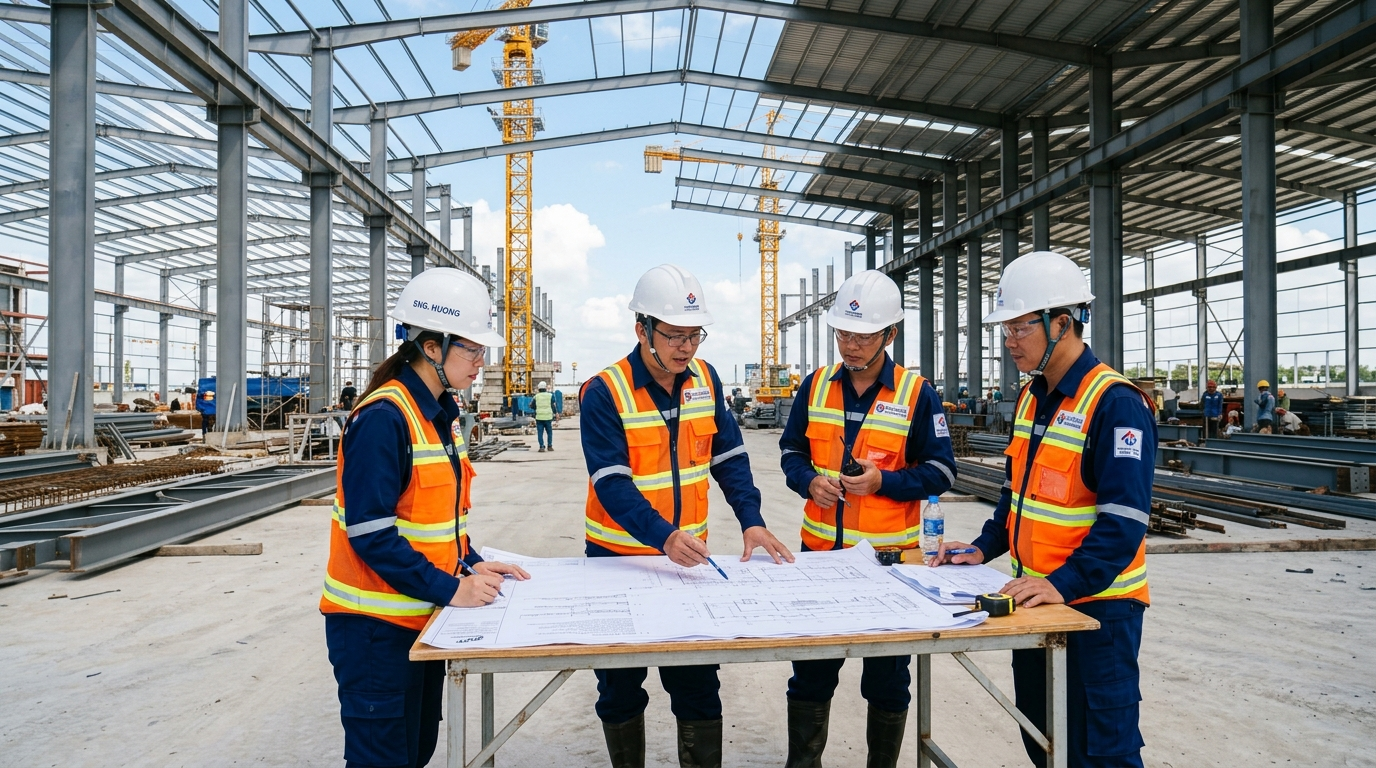
\includegraphics[width=186mm]{../../public/engineer-team-site.jpg}};
  \fill[TTCDeepNavy, opacity=0.82] (0,0) rectangle (68,72);
  \fill[TTCDeepNavy, opacity=0.38] (68,0) rectangle (92,72);

  \node[anchor=west, text width=54mm, align=left, text=white] at (8,48) {
    {\fontsize{7}{8}\selectfont\bfseries\color{TTCCyan} PEOPLE AT THE POINT OF EXECUTION}\\[1.5mm]
    {\fontsize{16}{18}\selectfont\bfseries PEOPLE IN\\EXECUTION SCORE}\\[2mm]
    {\fontsize{7.2}{9}\selectfont\color{white!84!gray}
    The project team is organized by task, with clear authority and a single reporting line.}
  };

  \node[
    anchor=south east, rounded corners=3pt,
    fill=white, fill opacity=0.93, text opacity=1,
    draw=TTCCyan, line width=0.7pt,
    minimum width=52mm, minimum height=14mm, align=center
  ] at (179,7) {
    {\fontsize{8}{9.5}\selectfont\bfseries\color{TTCBlue} FIELD-LED DECISION MAKING}\\[0.7mm]
    {\fontsize{6.5}{8}\selectfont\color{TTCTextDark}Technical decision to be taken near the site}
  };
  \draw[white, line width=1pt, rounded corners=3pt] (0.6,0.6) rectangle (185.4,71.4);
  \draw[TTCBorder, line width=0.65pt, rounded corners=3pt] (0,0) rectangle (186,72);
\end{tikzpicture}

\vspace{3mm}

% ACCOUNTABLE ROLES BY PROJECT PHASE
\noindent
\begin{tikzpicture}[x=1mm,y=1mm]
  \path[use as bounding box] (0,0) rectangle (186,67);
  \node[anchor=west, align=left] at (0,62) {
    {\fontsize{7}{8}\selectfont\bfseries\color{TTCCyan} PROJECT TEAM BY PHASE}\quad
    {\fontsize{9.5}{11}\selectfont\bfseries\color{TTCBlue} PHASED RESPONSIBILITY ROLE}
  };

  % Phase 01
  \fill[white, rounded corners=3pt] (0,0) rectangle (58,55);
  \draw[TTCBorder, line width=0.65pt, rounded corners=3pt] (0,0) rectangle (58,55);
  \fill[TTCLightBlue, rounded corners=3pt] (0,43) rectangle (58,55);
  \node[anchor=west] at (5,49) {
    {\fontsize{7}{8}\selectfont\bfseries\color{TTCCyan} 01 / PRE-CONSTRUCTION}
  };
  \node[anchor=north west, text width=48mm, align=left] at (5,39) {
    {\fontsize{9.5}{11}\selectfont\bfseries\color{TTCBlue} PREPARATION \& DESIGN}\\[1.2mm]
    {\fontsize{7}{8.6}\selectfont\color{TTCTextDark}
    \textbf{Project Director}\\
    The only focal point with Client.\\[0.8mm]
    \textbf{Design \& BIM Lead}\\
    Coordinate design, VE and model.\\[0.8mm]
    \textbf{Planning / QS / FIDIC}\\
    Lock range, schedule and budget.}
  };
  \node[anchor=south, align=center] at (29,3.5) {
    {\fontsize{6.5}{7.8}\selectfont\bfseries\color{TTCRed} OUTPUT: APPROVED BASELINE}
  };

  % Phase 02
  \fill[white, rounded corners=3pt] (64,0) rectangle (122,55);
  \draw[TTCBlue!55!white, line width=0.75pt, rounded corners=3pt] (64,0) rectangle (122,55);
  \fill[TTCBlue, rounded corners=3pt] (64,43) rectangle (122,55);
  \node[anchor=west] at (69,49) {
    {\fontsize{7}{8}\selectfont\bfseries\color{white} 02 / CONSTRUCTION}
  };
  \node[anchor=north west, text width=48mm, align=left] at (69,39) {
    {\fontsize{9.5}{11}\selectfont\bfseries\color{TTCBlue} SITE CONSTRUCTION}\\[1.2mm]
    {\fontsize{7}{8.6}\selectfont\color{TTCTextDark}
    \textbf{Construction / Site Manager}\\
    Resources • site • construction nose.\\[0.5mm]
    \textbf{Discipline Engineers}\\
    Structure • Infrastructure • MEP • Fire protection.\\[0.5mm]
    \textbf{HSE \& QA/QC Managers}\\
    Independent control.}
  };
  \node[anchor=south, align=center] at (93,2.5) {
    {\fontsize{6.5}{7.8}\selectfont\bfseries\color{TTCRed} OUTPUT: CONTROLLED EXECUTION}
  };

  % Phase 03
  \fill[white, rounded corners=3pt] (128,0) rectangle (186,55);
  \draw[TTCBorder, line width=0.65pt, rounded corners=3pt] (128,0) rectangle (186,55);
  \fill[TTCLightBlue, rounded corners=3pt] (128,43) rectangle (186,55);
  \node[anchor=west] at (133,49) {
    {\fontsize{7}{8}\selectfont\bfseries\color{TTCCyan} 03 / HANDOVER \& O\&M}
  };
  \node[anchor=north west, text width=48mm, align=left] at (133,39) {
    {\fontsize{9.5}{11}\selectfont\bfseries\color{TTCBlue} HANDOVER \& OPERATION}\\[1.2mm]
    {\fontsize{7}{8.6}\selectfont\color{TTCTextDark}
    \textbf{Commissioning Manager}\\
    Coordinate interlocking trials.\\[0.8mm]
    \textbf{As-built \& Digital Twin Team}\\
    Standardize asset records and data.\\[0.8mm]
    \textbf{Warranty Response Team}\\
    Receive and handle according to the contract conditions.}
  };
  \node[anchor=south, align=center] at (157,3.5) {
    {\fontsize{6.5}{7.8}\selectfont\bfseries\color{TTCRed} OUTPUT: READY FOR OPERATION}
  };
\end{tikzpicture}

\vspace{3mm}

% MOBILIZATION CHAIN — CLARIFIES HIERARCHY WITHOUT PORTRAIT PLACEHOLDERS
\noindent
\begin{tikzpicture}[x=1mm,y=1mm]
  \path[use as bounding box] (0,0) rectangle (186,29);
  \fill[TTCLightBlue, rounded corners=4pt] (0,0) rectangle (186,29);
  \draw[TTCBorder, line width=0.65pt, rounded corners=4pt] (0,0) rectangle (186,29);

  \node[align=center] at (22,14.5) {
    {\fontsize{6.5}{7.8}\selectfont\bfseries\color{TTCTextMuted} GOVERNANCE}\\[0.7mm]
    {\fontsize{9.2}{10.5}\selectfont\bfseries\color{TTCBlue} HEAD OFFICE PMO}\\[0.5mm]
    {\fontsize{6.4}{7.6}\selectfont Portfolio control}
  };
  \node[text=TTCRed] at (45,14.5) {\faChevronRight};
  \node[align=center] at (68,14.5) {
    {\fontsize{6.5}{7.8}\selectfont\bfseries\color{TTCTextMuted} ACCOUNTABILITY}\\[0.7mm]
    {\fontsize{9.2}{10.5}\selectfont\bfseries\color{TTCBlue} PROJECT DIRECTOR}\\[0.5mm]
    {\fontsize{6.4}{7.6}\selectfont Single point}
  };
  \node[text=TTCRed] at (93,14.5) {\faChevronRight};
  \node[align=center] at (118,14.5) {
    {\fontsize{6.5}{7.8}\selectfont\bfseries\color{TTCTextMuted} SITE AUTHORITY}\\[0.7mm]
    {\fontsize{9.2}{10.5}\selectfont\bfseries\color{TTCBlue} STEERING COMMITTEE}\\[0.5mm]
    {\fontsize{6.4}{7.6}\selectfont Daily execution}
  };
  \node[text=TTCRed] at (141,14.5) {\faChevronRight};
  \node[align=center] at (164,14.5) {
    {\fontsize{6.5}{7.8}\selectfont\bfseries\color{TTCTextMuted} DELIVERY}\\[0.7mm]
    {\fontsize{9.2}{10.5}\selectfont\bfseries\color{TTCRed} PROFESSIONAL TEAM}\\[0.5mm]
    {\fontsize{6.4}{7.6}\selectfont Task-based crews}
  };
\end{tikzpicture}

\vspace{3mm}

% CAPACITY SNAPSHOT
\noindent

\begin{tikzpicture}[x=1mm,y=1mm]
  \path[use as bounding box] (0,0) rectangle (186,27);
  \fill[white, rounded corners=4pt] (0,0) rectangle (186,27);
  \draw[TTCBorder, line width=0.65pt, rounded corners=4pt] (0,0) rectangle (186,27);
  \foreach \x in {46.5,93,139.5}{
    \draw[TTCBorder, line width=0.5pt] (\x,5) -- (\x,22);
  }
  \node[align=center] at (23.25,13.5) {
    {\fontsize{14}{15.5}\selectfont\bfseries\color{TTCRed} 350+}\\[0.8mm]
    {\fontsize{6.8}{8}\selectfont\bfseries\color{TTCTextDark} MANAGE \& Engineer}
  };
  \node[align=center] at (69.75,13.5) {
    {\fontsize{14}{15.5}\selectfont\bfseries\color{TTCBlue} 2.500+}\\[0.8mm]
    {\fontsize{6.8}{8}\selectfont\bfseries\color{TTCTextDark} TECHNICAL WORKERS}
  };
  \node[align=center] at (116.25,13.5) {
    {\fontsize{14}{15.5}\selectfont\bfseries\color{TTCCyan} 85+}\\[0.8mm]
    {\fontsize{6.8}{8}\selectfont\bfseries\color{TTCTextDark} COMMANDER \& MONITORING}
  };
  \node[align=center] at (162.75,13.5) {
    {\fontsize{14}{15.5}\selectfont\bfseries\color{TTCBlue} 60+}\\[0.8mm]
    {\fontsize{6.8}{8}\selectfont\bfseries\color{TTCTextDark} BIM engineer \& DIGITIZATION}
  };
\end{tikzpicture}
\end{minipage}
\newpage

% ============================================================
% PAGE 08: QUẢN TRỊ TÀI CHÍNH DỰ ÁN & KỶ LUẬT DÒNG TIỀN
% ============================================================
\pageheaderbar{PROJECT FINANCE \& CASH-FLOW DISCIPLINE}{Page 08}
\pagefooterbar{Page 08}

\begin{tikzpicture}[remember picture, overlay]
  \node[opacity=0.025, scale=2.6, font=\bfseries\sffamily, text=TTCBlue]
    at ([yshift=-12mm]current page.center) {FINANCIAL GOVERNANCE \& DISCIPLINE};
  \draw[TTCBlue!6!white, line width=0.45pt]
    ([xshift=15mm, yshift=20mm]current page.south west)
    grid[step=8mm]
    ([xshift=195mm, yshift=45mm]current page.south west);
\end{tikzpicture}

\begin{minipage}[t][246mm]{\textwidth}
\secbrand{Project Financial Management \& Cash Flow Discipline}{Project Financial Governance • Cost Discipline • Verified \& Traceable Records}

\vspace{1mm}
{\fontsize{14.5}{16.5}\selectfont\bfseries\color{TTCBlue}
CONTROL FROM THE CONTRACTOR RECEIPT DECISION TO THE FINAL SETTLEMENT OF THE PROJECT\par}
\vspace{1mm}
{\fontsize{7.5}{9}\selectfont\color{TTCTextMuted}
Each project is set up an independent budget, controlling 4 ports and reconciling periodically before mobilizing resources.\par}
\vspace{3.5mm}

% ============================================================
% TẦNG 1: BỐN CỔNG KIỂM SOÁT TÀI CHÍNH + NGUYÊN TẮC QUẢN TRỊ
% ============================================================
\noindent
\begin{tikzpicture}[x=1mm,y=1mm]
  \path[use as bounding box] (0,0) rectangle (186,86);

  % KHỐI TRÁI: 4 CỔNG KIỂM SOÁT (126mm x 86mm)
  \fill[white, rounded corners=4pt] (0,0) rectangle (126,86);
  \draw[TTCBorder, line width=0.7pt, rounded corners=4pt] (0,0) rectangle (126,86);

  \node[anchor=west, text=TTCCyan, font=\fontsize{7}{8}\selectfont\bfseries]
    at (6,79.5) {FOUR FINANCIAL CONTROL GATES};
  \node[anchor=west, text=TTCBlue, font=\fontsize{10}{12}\selectfont\bfseries]
    at (6,72.5) {FOUR PROJECT FINANCIAL CONTROL GATES};

  % Timeline connector bar
  \draw[TTCBlue!30!white, line width=1pt] (15,50) -- (111,50);

  % 4 Cổng Nodes & Contents
  % Cổng 01
  \fill[TTCRed] (15,50) circle (4.8);
  \node[text=white, font=\fontsize{7}{8}\selectfont\bfseries] at (15,50) {01};
  \node[anchor=south, align=center, text width=26mm, text=TTCRed, font=\fontsize{7}{8.2}\selectfont\bfseries]
    at (15,57.5) {APPRAISAL\\CONTRACT};
  \node[anchor=north, align=center, text width=27mm, text=TTCTextDark, font=\fontsize{6.2}{7.6}\selectfont]
    at (15,42.5) {Profit Margin\\Payment Terms\\Retention risk};

  % Cổng 02
  \fill[white] (47,50) circle (4.8);
  \draw[TTCBlue, line width=0.85pt] (47,50) circle (4.8);
  \node[text=TTCBlue, font=\fontsize{7}{8}\selectfont\bfseries] at (47,50) {02};
  \node[anchor=south, align=center, text width=26mm, text=TTCBlue, font=\fontsize{7}{8.2}\selectfont\bfseries]
    at (47,57.5) {BUDGET\\Project};
  \node[anchor=north, align=center, text width=27mm, text=TTCTextDark, font=\fontsize{6.2}{7.6}\selectfont]
    at (47,42.5) {Baseline costs\\Cash flow plan\\Disbursement limits};

  % Cổng 03
  \fill[white] (79,50) circle (4.8);
  \draw[TTCBlue, line width=0.85pt] (79,50) circle (4.8);
  \node[text=TTCBlue, font=\fontsize{7}{8}\selectfont\bfseries] at (79,50) {03};
  \node[anchor=south, align=center, text width=26mm, text=TTCBlue, font=\fontsize{7}{8.2}\selectfont\bfseries]
    at (79,57.5) {CONTROL\\IMPLEMENTATION};
  \node[anchor=north, align=center, text width=27mm, text=TTCTextDark, font=\fontsize{6.2}{7.6}\selectfont]
    at (79,42.5) {Plan Reality Comparison\\Additional Approval (VO)\\Forecast Completion (EAC)};

  % Cổng 04
  \fill[white] (111,50) circle (4.8);
  \draw[TTCBlue, line width=0.85pt] (111,50) circle (4.8);
  \node[text=TTCBlue, font=\fontsize{7}{8}\selectfont\bfseries] at (111,50) {04};
  \node[anchor=south, align=center, text width=26mm, text=TTCBlue, font=\fontsize{7}{8.2}\selectfont\bfseries]
    at (111,57.5) {ACCEPTANCE\\SETTLEMENT};
  \node[anchor=north, align=center, text width=27mm, text=TTCTextDark, font=\fontsize{6.2}{7.6}\selectfont]
    at (111,42.5) {As-built Bill of Quantities\\Debt collection\\Close project cost code};

  % Dải cam kết phía dưới khối trái
  \fill[TTCDeepNavy, rounded corners=3pt] (5,5.5) rectangle (121,18.5);
  \node[anchor=west, text=TTCCyan, font=\fontsize{6.8}{8}\selectfont\bfseries]
    at (8,12) {\faShield*\quad CONTROL BEFORE COMMITMENT};
  \node[anchor=east, text=white, font=\fontsize{6.5}{7.8}\selectfont\bfseries]
    at (118,12) {Only commit when budgeted \& approved cash flow};

  % KHỐI PHẢI: NGUYÊN TẮC QUẢN TRỊ (55mm x 86mm)
  \fill[TTCLightBlue, rounded corners=4pt] (131,0) rectangle (186,86);
  \draw[TTCBorder, line width=0.7pt, rounded corners=4pt] (131,0) rectangle (186,86);

  \node[anchor=north west, text=TTCCyan, font=\fontsize{7}{8}\selectfont\bfseries]
    at (136,79.5) {CONTROL PRINCIPLE};
  \node[anchor=north west, text width=46mm, text=TTCBlue, font=\fontsize{9.5}{11.5}\selectfont\bfseries]
    at (136,73) {DO NOT RECEIVE BIDS EXCEEDING PROFILE};
  \fill[TTCRed] (136,61.5) rectangle (152,63);

  \node[anchor=north west, text width=45mm, text=TTCTextDark, font=\fontsize{6.8}{8.6}\selectfont]
    at (136,56) {
    \textcolor{TTCRed}{\faCheckCircle}\ \textbf{Budget Lock:} Approval before resource mobilization.\\[2.4mm]
    \textcolor{TTCRed}{\faCheckCircle}\ \textbf{Arising control:} Any non-contractual costs must be approved.\\[2.4mm]
    \textcolor{TTCRed}{\faCheckCircle}\ \textbf{safety growth:} Scale only expands when handover is ready.
  };

  \fill[white, rounded corners=2.5pt, draw=TTCBorder, line width=0.55pt] (136,6) rectangle (181,18);
  \node[anchor=center, text=TTCBlue, font=\fontsize{6.6}{8}\selectfont\bfseries, align=center]
    at (158.5,12) {\faLock\quad EACH PROJECT HAS ITS OWN COST CODE};
\end{tikzpicture}

\vspace{3.5mm}

% ============================================================
% TẦNG 2: BA TRỤ CỘT QUẢN TRỊ TÀI CHÍNH
% ============================================================
\noindent
\begin{tikzpicture}[x=1mm,y=1mm]
  \path[use as bounding box] (0,0) rectangle (186,58);

  % 3 Cột: Kiểm soát chi phí | Kiểm soát công nợ | Hồ sơ truy xuất (58mm mỗi cột)
  % Card 1: Cost Control
  \fill[white, rounded corners=4pt] (0,0) rectangle (58,58);
  \draw[TTCBorder, line width=0.65pt, rounded corners=4pt] (0,0) rectangle (58,58);
  \fill[TTCRed, rounded corners=1pt] (5,50.5) rectangle (22,52.5);
  \node[anchor=north west, text width=50mm, align=left] at (5,47.5) {
    {\fontsize{7}{8.2}\selectfont\bfseries\color{TTCRed}\faCalculator\quad COST CONTROL}\\[1.2mm]
    {\fontsize{9.8}{11.5}\selectfont\bfseries\color{TTCBlue} COST CONTROL}\\[2mm]
    {\fontsize{6.6}{8.2}\selectfont\color{TTCTextDark}
    \textbullet\ Establish a baseline budget according to the WBS.\newline
    \textbullet\ Report weekly expense variance.\newline
    \textbullet\ Forecast of total cost of completion (EAC).}
  };

  % Card 2: Receivable Control
  \fill[white, rounded corners=4pt] (64,0) rectangle (122,58);
  \draw[TTCBorder, line width=0.65pt, rounded corners=4pt] (64,0) rectangle (122,58);
  \fill[TTCCyan, rounded corners=1pt] (69,50.5) rectangle (86,52.5);
  \node[anchor=north west, text width=50mm, align=left] at (69,47.5) {
    {\fontsize{7}{8.2}\selectfont\bfseries\color{TTCCyan}\faFileInvoiceDollar\quad RECEIVABLE CONTROL}\\[1.2mm]
    {\fontsize{9.8}{11.5}\selectfont\bfseries\color{TTCBlue} DEBT CONTROL}\\[2mm]
    {\fontsize{6.6}{8.2}\selectfont\color{TTCTextDark}
    \textbullet\ Closely follow the inspection plan.\newline
    \textbullet\ Payment cash flow tracking \& advance payment.\newline
    \textbullet\ Strictly administer the warranty retention.}
  };

  % Card 3: Verified Reporting
  \fill[white, rounded corners=4pt] (128,0) rectangle (186,58);
  \draw[TTCBorder, line width=0.65pt, rounded corners=4pt] (128,0) rectangle (186,58);
  \fill[TTCBlue, rounded corners=1pt] (133,50.5) rectangle (150,52.5);
  \node[anchor=north west, text width=50mm, align=left] at (133,47.5) {
    {\fontsize{7}{8.2}\selectfont\bfseries\color{TTCBlue}\faClipboardCheck\quad VERIFIED REPORTING}\\[1.2mm]
    {\fontsize{9.8}{11.5}\selectfont\bfseries\color{TTCBlue} COMPANY RETRIEVAL}\\[2mm]
    {\fontsize{6.6}{8.2}\selectfont\color{TTCTextDark}
    \textbullet\ Cost data updated by admin cycle.\newline
    \textbullet\ Report variance and forecast completion.\newline
    \textbullet\ Detailed documents provided on request Client.}
  };
\end{tikzpicture}

\vspace{3.5mm}

% ============================================================
% TẦNG 3: GÓI HỒ SƠ MINH CHỨNG & CHÍNH SÁCH BẢO MẬT
% ============================================================
\noindent
\begin{tikzpicture}[x=1mm,y=1mm]
  \path[use as bounding box] (0,0) rectangle (186,46);

  % Outer Card
  \fill[white, rounded corners=4pt] (0,0) rectangle (186,46);
  \draw[TTCBorder, line width=0.65pt, rounded corners=4pt] (0,0) rectangle (186,46);

  % Left Navy Brand Anchor (48mm x 46mm)
  \fill[TTCDeepNavy, rounded corners=4pt] (0,0) rectangle (48,46);
  \node[anchor=west, text width=40mm, align=left] at (6,23) {
    {\fontsize{7}{8}\selectfont\bfseries\color{TTCCyan} DISCLOSURE POLICY}\\[1.2mm]
    {\fontsize{9}{11}\selectfont\bfseries\color{white} TRANSPARENCY YES\\CONTROL}\\[1.8mm]
    {\fontsize{6}{7.2}\selectfont\color{white!75!gray}Verified data \textbullet\ Right audience}
  };

  % 4 Pill Cards on the Right
  \foreach \xa/\xb/\num/\label/\sub in {
    53/81/01/FINANCIAL REPORT/Independent auditor,
    85/113/02/COMPANY TAX/State Obligations,
    117/145/03/DEBT RECONCILIATION/Supplier and sub-contractor,
    149/181/04/GOVERNANCE REPORT/Project cash flow}{
    \fill[TTCLightBlue, rounded corners=3pt] (\xa,14) rectangle (\xb,40);
    \draw[TTCBorder, line width=0.5pt, rounded corners=3pt] (\xa,14) rectangle (\xb,40);
    \node[text=TTCRed, font=\fontsize{8}{9.5}\selectfont\bfseries] at ({(\xa+\xb)/2},34.5) {\num};
    \node[align=center, text width=26mm, text=TTCBlue, font=\fontsize{6.5}{7.8}\selectfont\bfseries]
      at ({(\xa+\xb)/2},26) {\label};
    \node[align=center, text width=26mm, text=TTCTextMuted, font=\fontsize{5.8}{7}\selectfont]
      at ({(\xa+\xb)/2},18.5) {\sub};
  }

  % Bottom Security Notice
  \draw[TTCBorder, line width=0.5pt] (53,9.5) -- (181,9.5);
  \node[anchor=south west, text=TTCTextMuted, font=\fontsize{6}{7.3}\selectfont\itshape]
    at (53,3) {\faLock\quad Detailed data is only provided according to the bidding documents or confidentiality agreement with Client.};
\end{tikzpicture}
\end{minipage}
\newpage

% ============================================================
% PAGE 09: BẢO LÃNH HỢP ĐỒNG & HUY ĐỘNG NGUỒN LỰC
% ============================================================
\pageheaderbar{CONTRACT GUARANTEES \& RESOURCE MOBILIZATION}{Page 09}
\pagefooterbar{Page 09}

\begin{tikzpicture}[remember picture, overlay]
  \node[opacity=0.02, scale=2.4, font=\bfseries\sffamily, text=TTCBlue]
    at ([yshift=-12mm]current page.center) {BANKING CAPACITY \& SITE MOBILIZATION};
  \draw[TTCBlue!6!white, line width=0.45pt]
    ([xshift=15mm, yshift=20mm]current page.south west)
    grid[step=8mm]
    ([xshift=195mm, yshift=45mm]current page.south west);
\end{tikzpicture}

\begin{minipage}[t][246mm]{\textwidth}
\secbrand{Guaranteed Qualification \& Project Mobilization}{Banking Readiness, Contract Security \& Workforce Mobilization}

\vspace{1mm}
{\fontsize{14.5}{16.5}\selectfont\bfseries\color{TTCBlue}
TWO RESOURCES • A COMPREHENSIVE MOBILIZATION PLAN\par}
\vspace{1mm}
{\fontsize{7.5}{9}\selectfont\color{TTCTextMuted}
Bank records and personnel plans are prepared according to each contract milestone, scope of work and mobilization requirements.\par}
\vspace{3.5mm}

% ============================================================
% TẦNG 1: HAI ĐỘNG CƠ HUY ĐỘNG (FINANCIAL ENGINE & DELIVERY ENGINE)
% ============================================================
\noindent
\begin{tikzpicture}[x=1mm,y=1mm]
  \path[use as bounding box] (0,0) rectangle (186,80);

  % KHỐI TRÁI: HỒ SƠ NGÂN HÀNG VÀ BẢO LÃNH
  \fill[white, rounded corners=4pt] (0,0) rectangle (90,80);
  \draw[TTCBorder, line width=0.7pt, rounded corners=4pt] (0,0) rectangle (90,80);

  \node[anchor=north west, text=TTCCyan, font=\fontsize{7}{8}\selectfont\bfseries]
    at (6,73.5) {FINANCIAL ENGINE};
  \node[anchor=north west, text=TTCBlue, font=\fontsize{10}{12}\selectfont\bfseries]
    at (6,67) {PROFILE TRUST AVAILABLE \& GUARANTEE};

  \node[anchor=west] at (6,54) {
    {\fontsize{16}{19}\selectfont\bfseries\color{TTCRed} COMPANY READY}\quad
    {\fontsize{7.5}{9}\selectfont\bfseries\color{TTCTextMuted} ACCORDING TO THE CONTRACT REQUIREMENTS}
  };

  % Bank Badges
  \fill[TTCLightBlue, rounded corners=2.5pt, draw=TTCBorder, line width=0.5pt] (5,38) rectangle (85,46);
  \node[anchor=center, text=TTCBlue, font=\fontsize{6.2}{7.4}\selectfont\bfseries]
    at (45,42) {Vietcombank \textbullet\ BIDV \textbullet\ VietinBank \textbullet\ TPBank \textbullet\ ACB \textbullet\ MB};

  \node[anchor=north west, text width=80mm, text=TTCTextDark, font=\fontsize{6.8}{8.6}\selectfont]
    at (6,33.5) {
    \textcolor{TTCRed}{\faCheckCircle}\ \textbf{Type of guarantee:} Bid, execution, advance and warranty.\\[1.4mm]
    \textcolor{TTCRed}{\faCheckCircle}\ \textbf{Issuance conditions:} According to bank approval and contract documents.\\[1.4mm]
    \textcolor{TTCRed}{\faCheckCircle}\ \textbf{Reconciliation documents:} Confirm the bank provided in the prequalification dossier when required.
  };

  % KHỐI PHẢI: KẾ HOẠCH HUY ĐỘNG NHÂN SỰ
  \fill[white, rounded corners=4pt] (96,0) rectangle (186,80);
  \draw[TTCBorder, line width=0.7pt, rounded corners=4pt] (96,0) rectangle (186,80);

  \node[anchor=north west, text=TTCCyan, font=\fontsize{7}{8}\selectfont\bfseries]
    at (102,73.5) {DELIVERY ENGINE};
  \node[anchor=north west, text=TTCBlue, font=\fontsize{10}{12}\selectfont\bfseries]
    at (102,67) {FIELD DEPLOYMENT FORCES};

  \node[anchor=west] at (102,54) {
    {\fontsize{16}{19}\selectfont\bfseries\color{TTCBlue} BY WORK PACKAGE}\quad
    {\fontsize{7.5}{9}\selectfont\bfseries\color{TTCTextMuted} MOBILIZATION PLAN}
  };

  % Visual Distribution Bar
  \fill[TTCBlue, rounded corners=1.5pt] (102,41) rectangle (126,45);
  \fill[TTCCyan, rounded corners=1.5pt] (127,41) rectangle (151,45);
  \fill[TTCRed, rounded corners=1.5pt] (152,41) rectangle (180,45);
  \node[anchor=west, text=TTCBlue, font=\fontsize{6.1}{7.3}\selectfont\bfseries] at (102,47.5) {PROJECT MANAGER • ENGINEER • CONSTRUCTION TEAM};

  \node[anchor=north west, text width=78mm, text=TTCTextDark, font=\fontsize{6.8}{8.6}\selectfont]
    at (102,33.5) {
    \textcolor{TTCBlue}{\faCheckCircle}\ \textbf{Key personnel:} Practicing certificates suitable to the position and scope of work.\\[1.4mm]
    \textcolor{TTCCyan}{\faCheckCircle}\ \textbf{Professional team:} Welding, structural, electromechanical and fire prevention \& fighting erection.\\[1.4mm]
    \textcolor{TTCTextMuted}{\faCheckCircle}\ \textbf{Construction organization:} The scale and shift are locked in the approved mobilization plan.
  };

  % Joining Connector Pill
  \fill[white] (93,54) circle (4);
  \draw[TTCCyan, line width=0.8pt] (93,54) circle (4);
  \node[text=TTCRed, font=\fontsize{10}{11}\selectfont\bfseries] at (93,54) {+};
\end{tikzpicture}

\vspace{3.5mm}

% ============================================================
% TẦNG 2: 4 GIAI ĐOẠN KÍCH HOẠT HỢP ĐỒNG (CONTRACT LIFECYCLE)
% ============================================================
\noindent
\begin{tikzpicture}[x=1mm,y=1mm]
  \path[use as bounding box] (0,0) rectangle (186,84);

  \node[anchor=west] at (0,79) {
    {\fontsize{7}{8}\selectfont\bfseries\color{TTCCyan} CONTRACT LIFECYCLE}\quad
    {\fontsize{9.8}{11.5}\selectfont\bfseries\color{TTCBlue} RESOURCES ARE TRIGGERED IN STAGES}
  };

  % 4 Stages: 01 Tender | 02 Award | 03 Delivery | 04 Handover (42.5mm mỗi card)
  % Stage 01: Tender
  \fill[white, rounded corners=3.5pt] (0,0) rectangle (42,72);
  \draw[TTCBorder, line width=0.65pt, rounded corners=3.5pt] (0,0) rectangle (42,72);
  \fill[TTCLightBlue, rounded corners=3.5pt] (0,59) rectangle (42,72);
  \node[anchor=west] at (4,65.5) {
    {\fontsize{7}{8}\selectfont\bfseries\color{TTCCyan} 01 / TENDER}
  };
  \node[anchor=north west, text width=34mm, align=left] at (4,53) {
    {\fontsize{9.8}{11.5}\selectfont\bfseries\color{TTCBlue} BID}\\[2.2mm]
    {\fontsize{6.5}{7.8}\selectfont\bfseries\color{TTCTextMuted} FINANCE}\\[0.7mm]
    {\fontsize{6.8}{8.2}\selectfont\color{TTCTextDark}Bid Security in accordance with the requirements of the bidding documents.}\\[2mm]
    {\fontsize{6.5}{7.8}\selectfont\bfseries\color{TTCTextMuted} HUMAN RESOURCES}\\[0.7mm]
    {\fontsize{6.8}{8.2}\selectfont\color{TTCTextDark}Bidding, cost estimation, value engineering and contracts.}
  };
  \fill[TTCLightBlue, rounded corners=2pt, draw=TTCBorder, line width=0.5pt] (6,3.5) rectangle (36,10);
  \node[anchor=center] at (21,6.75) {
    {\fontsize{6.4}{7.8}\selectfont\bfseries\color{TTCBlue} BID-READY}
  };

  % Chevron 1 -> 2
  \node[text=TTCRed] at (45,36) {\faChevronRight};

  % Stage 02: Award
  \fill[white, rounded corners=3.5pt] (48,0) rectangle (90,72);
  \draw[TTCBorder, line width=0.65pt, rounded corners=3.5pt] (48,0) rectangle (90,72);
  \fill[TTCLightBlue, rounded corners=3.5pt] (48,59) rectangle (90,72);
  \node[anchor=west] at (52,65.5) {
    {\fontsize{7}{8}\selectfont\bfseries\color{TTCCyan} 02 / AWARD}
  };
  \node[anchor=north west, text width=34mm, align=left] at (52,53) {
    {\fontsize{9.8}{11.5}\selectfont\bfseries\color{TTCBlue} SIGNING THE CONTRACT}\\[2.2mm]
    {\fontsize{6.5}{7.8}\selectfont\bfseries\color{TTCTextMuted} FINANCE}\\[0.7mm]
    {\fontsize{6.8}{8.2}\selectfont\color{TTCTextDark}Performance guarantee and advance payment under the contract.}\\[2mm]
    {\fontsize{6.5}{7.8}\selectfont\bfseries\color{TTCTextMuted} HUMAN RESOURCES}\\[0.7mm]
    {\fontsize{6.8}{8.2}\selectfont\color{TTCTextDark}Appointment of Project Director and key personnel team.}
  };
  \fill[TTCLightBlue, rounded corners=2pt, draw=TTCBorder, line width=0.5pt] (54,3.5) rectangle (84,10);
  \node[anchor=center] at (69,6.75) {
    {\fontsize{6.4}{7.8}\selectfont\bfseries\color{TTCBlue} CONTRACT-READY}
  };

  % Chevron 2 -> 3
  \node[text=TTCRed] at (93,36) {\faChevronRight};

  % Stage 03: Delivery
  \fill[white, rounded corners=3.5pt] (96,0) rectangle (138,72);
  \draw[TTCBlue!60!white, line width=0.75pt, rounded corners=3.5pt] (96,0) rectangle (138,72);
  \fill[TTCBlue, rounded corners=3.5pt] (96,59) rectangle (138,72);
  \node[anchor=west] at (100,65.5) {
    {\fontsize{7}{8}\selectfont\bfseries\color{white} 03 / DELIVERY}
  };
  \node[anchor=north west, text width=34mm, align=left] at (100,53) {
    {\fontsize{9.8}{11.5}\selectfont\bfseries\color{TTCBlue} IMPLEMENTATION}\\[2.2mm]
    {\fontsize{6.5}{7.8}\selectfont\bfseries\color{TTCTextMuted} FINANCE}\\[0.7mm]
    {\fontsize{6.8}{8.2}\selectfont\color{TTCTextDark}Working capital, procurement of materials and payment of suppliers.}\\[2mm]
    {\fontsize{6.5}{7.8}\selectfont\bfseries\color{TTCTextMuted} HUMAN RESOURCES}\\[0.7mm]
    {\fontsize{6.8}{8.2}\selectfont\color{TTCTextDark}Commanders, field engineers and teams according to schedule.}
  };
  \fill[TTCBlue, rounded corners=2pt] (102,3.5) rectangle (132,10);
  \node[anchor=center] at (117,6.75) {
    {\fontsize{6.4}{7.8}\selectfont\bfseries\color{white} SITE-READY}
  };

  % Chevron 3 -> 4
  \node[text=TTCRed] at (141,36) {\faChevronRight};

  % Stage 04: Handover
  \fill[white, rounded corners=3.5pt] (144,0) rectangle (186,72);
  \draw[TTCRed!70!white, line width=0.75pt, rounded corners=3.5pt] (144,0) rectangle (186,72);
  \fill[TTCRed, rounded corners=3.5pt] (144,59) rectangle (186,72);
  \node[anchor=west] at (148,65.5) {
    {\fontsize{7}{8}\selectfont\bfseries\color{white} 04 / HANDOVER}
  };
  \node[anchor=north west, text width=34mm, align=left] at (148,53) {
    {\fontsize{9.8}{11.5}\selectfont\bfseries\color{TTCBlue} HANDOVER}\\[2.2mm]
    {\fontsize{6.5}{7.8}\selectfont\bfseries\color{TTCTextMuted} FINANCE}\\[0.7mm]
    {\fontsize{6.8}{8.2}\selectfont\color{TTCTextDark}Warranty guarantee according to contract conditions.}\\[2mm]
    {\fontsize{6.5}{7.8}\selectfont\bfseries\color{TTCTextMuted} HUMAN RESOURCES}\\[0.7mm]
    {\fontsize{6.8}{8.2}\selectfont\color{TTCTextDark}Commissioning, as-built documents and receipt of warranty.}
  };
  \fill[TTCRed, rounded corners=2pt] (150,3.5) rectangle (180,10);
  \node[anchor=center] at (165,6.75) {
    {\fontsize{6.4}{7.8}\selectfont\bfseries\color{white} O\&M-READY}
  };
\end{tikzpicture}

\vspace{3.5mm}

% ============================================================
% TẦNG 3: BĂNG CAM KẾT SẴN SÀNG HUY ĐỘNG (MOBILIZATION ASSURANCE)
% ============================================================
\noindent
\begin{tikzpicture}[x=1mm,y=1mm]
  \path[use as bounding box] (0,0) rectangle (186,43);

  % Outer Card
  \fill[white, rounded corners=4pt] (0,0) rectangle (186,43);
  \draw[TTCBorder, line width=0.65pt, rounded corners=4pt] (0,0) rectangle (186,43);

  % Left Navy Brand Anchor (48mm x 43mm)
  \fill[TTCDeepNavy, rounded corners=4pt] (0,0) rectangle (48,43);
  \node[anchor=west, text width=40mm, align=left] at (6,21.5) {
    {\fontsize{7}{8}\selectfont\bfseries\color{TTCCyan} ASSURANCE}\\[1mm]
    {\fontsize{8.8}{10.5}\selectfont\bfseries\color{white} CONDITION\\READY}\\[1.5mm]
    {\fontsize{6}{7.2}\selectfont\color{white!75!gray}Financial \textbullet\ Technical \textbullet\ HSE}
  };

  % 4 Metric Badges on Right
  \foreach \xa/\xb/\val/\title/\sub in {
    53/81/COMPANY/TRUST APPLIED/Reconciled upon request,
    85/113/TRAINING/SAFETY SAFETY/Before entering the construction site,
    117/145/CERTIFICATE/WELDER/According to technical requirements,
    149/181/LANGUAGE/COORDINATION/Vietnamese • English by project}{
    \fill[TTCLightBlue, rounded corners=3pt] (\xa,4.5) rectangle (\xb,38.5);
    \draw[TTCBorder, line width=0.5pt, rounded corners=3pt] (\xa,4.5) rectangle (\xb,38.5);
    \node[text=TTCRed, font=\fontsize{11}{13}\selectfont\bfseries] at ({(\xa+\xb)/2},29.5) {\val};
    \node[align=center, text width=26mm, text=TTCBlue, font=\fontsize{6.4}{7.6}\selectfont\bfseries]
      at ({(\xa+\xb)/2},19.5) {\title};
    \node[align=center, text width=26mm, text=TTCTextMuted, font=\fontsize{5.8}{7}\selectfont]
      at ({(\xa+\xb)/2},11) {\sub};
  }
\end{tikzpicture}
\end{minipage}
\newpage

% ============================================================
% PAGE 10: TALENT DEVELOPMENT JOURNEY & SAFETY CULTURE
% ============================================================
\pageheaderbar{CAPABILITY DEVELOPMENT \& SAFETY CULTURE}{Page 10}
\pagefooterbar{Page 10}

\begin{tikzpicture}[remember picture, overlay]
  \node[opacity=0.02, scale=2.4, font=\bfseries\sffamily, text=TTCBlue]
    at ([yshift=-12mm]current page.center) {TALENT DEVELOPMENT \& SAFETY CULTURE};
  \draw[TTCBlue!6!white, line width=0.45pt]
    ([xshift=15mm, yshift=20mm]current page.south west)
    grid[step=8mm]
    ([xshift=195mm, yshift=45mm]current page.south west);
\end{tikzpicture}

\begin{minipage}[t][246mm]{\textwidth}
\secbrand{Capability Development Pathway}{Talent Development, Technical Certification \& Safety-First Culture}

\vspace{1mm}
{\fontsize{14.5}{16.5}\selectfont\bfseries\color{TTCBlue}
LEARNING THE RIGHT THING • CERTIFYING THE RIGHT STANDARDS • LEADING THE PROJECT\par}
\vspace{1mm}
{\fontsize{7.5}{9}\selectfont\color{TTCTextMuted}
The training system is associated with field operations, turning professional knowledge into construction results of safety.\par}
\vspace{3.5mm}

% ============================================================
% TRAINING HERO BANNER
% ============================================================
\noindent
\begin{tikzpicture}[x=1mm,y=1mm]
  \path[use as bounding box] (0,0) rectangle (186,65);
  \clip[rounded corners=3pt] (0,0) rectangle (186,65);
  \node[anchor=center, inner sep=0pt] at (93,32.5)
    {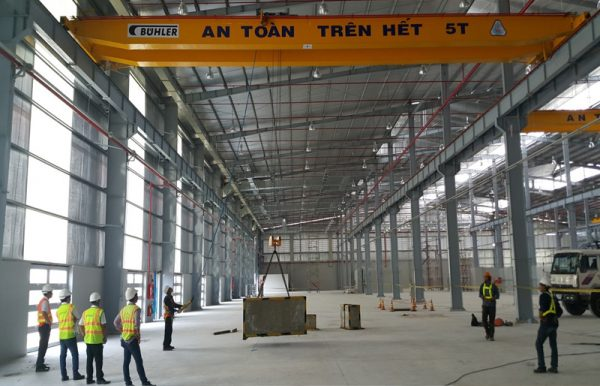
\includegraphics[width=186mm]{../../public/introsection1.jpg}};
  \fill[TTCDeepNavy, opacity=0.84] (0,0) rectangle (74,65);
  \fill[TTCDeepNavy, opacity=0.28] (74,0) rectangle (98,65);
  \node[anchor=west, text width=60mm, align=left, text=white] at (8,43) {
    {\fontsize{7}{8}\selectfont\bfseries\color{TTCCyan} FIELD-BASED LEARNING}\\[1.4mm]
    {\fontsize{15}{17}\selectfont\bfseries STUDY IN\\EXECUTION SCORE}\\[1.8mm]
    {\fontsize{7}{8.6}\selectfont\color{white!82!gray}
    Training is associated with real situations, real equipment and the right to stop work when safety is not available.}
  };
  \node[
    anchor=south east, rounded corners=3pt,
    fill=white, fill opacity=0.94, text opacity=1,
    draw=TTCCyan, line width=0.65pt,
    minimum width=52mm, minimum height=13mm, align=center
  ] at (179,7) {
    {\fontsize{8.2}{9.5}\selectfont\bfseries\color{TTCBlue} SAFETY BEFORE PRODUCTIVITY}\\[0.6mm]
    {\fontsize{6.4}{7.8}\selectfont\color{TTCTextDark}Safety is a prerequisite for starting work}
  };
  \draw[white, line width=1pt, rounded corners=3pt] (0.6,0.6) rectangle (185.4,64.4);
  \draw[TTCBorder, line width=0.65pt, rounded corners=3pt] (0,0) rectangle (186,65);
\end{tikzpicture}

\vspace{3.5mm}

% ============================================================
% DEVELOPMENT JOURNEY (LỘ TRÌNH NĂNG LỰC)
% ============================================================
\noindent
\begin{tikzpicture}[x=1mm,y=1mm]
  \path[use as bounding box] (0,0) rectangle (186,53);
  \node[anchor=west] at (0,48) {
    {\fontsize{7}{8}\selectfont\bfseries\color{TTCCyan} DEVELOPMENT JOURNEY}\quad
    {\fontsize{9.5}{11}\selectfont\bfseries\color{TTCBlue} ROADMAP PROFILE FROM THE FIELD TO THE LEADER}
  };
  \draw[TTCBlue!28!white, line width=0.8pt] (22,30) -- (164,30);

  \foreach \x/\num in {22/01,69/02,117/03,164/04}{
    \fill[white] (\x,30) circle (5);
    \draw[TTCBlue!45!white, line width=0.75pt] (\x,30) circle (5);
    \node[text=TTCBlue, font=\fontsize{7}{8}\selectfont\bfseries] at (\x,30) {\num};
  }
  \fill[TTCRed] (164,30) circle (5);
  \node[text=white, font=\fontsize{7}{8}\selectfont\bfseries] at (164,30) {04};

  \node[align=center, text width=36mm] at (22,13) {
    {\fontsize{8.8}{10}\selectfont\bfseries\color{TTCBlue} HSE READY}\\[0.7mm]
    {\fontsize{6.5}{7.8}\selectfont Required training before entering the site}
  };
  \node[align=center, text width=36mm] at (69,13) {
    {\fontsize{8.8}{10}\selectfont\bfseries\color{TTCBlue} TECHNICAL MASTERY}\\[0.7mm]
    {\fontsize{6.5}{7.8}\selectfont BIM • Tekla • MEP • PEB • QA/QC}
  };
  \node[align=center, text width=36mm] at (117,13) {
    {\fontsize{8.8}{10}\selectfont\bfseries\color{TTCBlue} CERTIFIED PRO}\\[0.7mm]
    {\fontsize{6.5}{7.8}\selectfont Class II • AWS D1.1 • PMP • FIDIC}
  };
  \node[align=center, text width=36mm] at (164,13) {
    {\fontsize{8.8}{10}\selectfont\bfseries\color{TTCRed} PROJECT LEADER}\\[0.7mm]
    {\fontsize{6.5}{7.8}\selectfont Lead, coach, and lead your team}
  };
\end{tikzpicture}

\vspace{3.5mm}

% ============================================================
% TWO DEVELOPMENT SYSTEMS
% ============================================================
\noindent
\begin{tikzpicture}[x=1mm,y=1mm]
  \path[use as bounding box] (0,0) rectangle (186,49);
  \fill[white, rounded corners=4pt] (0,0) rectangle (91,49);
  \draw[TTCBorder, line width=0.65pt, rounded corners=4pt] (0,0) rectangle (91,49);
  \node[anchor=north west, text width=79mm, align=left] at (6,43) {
    {\fontsize{7}{8}\selectfont\bfseries\color{TTCCyan} TTC TECHNICAL ACADEMY}\\[0.8mm]
    {\fontsize{10}{11.5}\selectfont\bfseries\color{TTCBlue} PROFILE EXPERTISE}\\[1.5mm]
    {\fontsize{6.8}{8.4}\selectfont\color{TTCTextDark}
    \textcolor{TTCCyan}{\faCheckCircle}\ \textbf{ConTech \& BIM:} Revit, Tekla LOD 400, Navisworks, CDE.\\[0.8mm]
    \textcolor{TTCCyan}{\faCheckCircle}\ \textbf{Technical trades:} AWS D1.1, MEP/fire prevention and fighting, working at height.\\[0.8mm]
    \textcolor{TTCCyan}{\faCheckCircle}\ \textbf{Project control:} PMP, FIDIC, QS and schedule plan.}
  };

  \fill[TTCLightBlue, rounded corners=4pt] (95,0) rectangle (186,49);
  \draw[TTCBorder, line width=0.65pt, rounded corners=4pt] (95,0) rectangle (186,49);
  \node[anchor=north west, text width=79mm, align=left] at (101,43) {
    {\fontsize{7}{8}\selectfont\bfseries\color{TTCRed} SAFETY \& CULTURE SYSTEM}\\[0.8mm]
    {\fontsize{10}{11.5}\selectfont\bfseries\color{TTCBlue} BEHAVIOR \& BENEFITS}\\[1.5mm]
    {\fontsize{6.8}{8.4}\selectfont\color{TTCTextDark}
    \textcolor{TTCRed}{\faCheckCircle}\ Toolbox talk, fire drill and rescue periodically.\\[0.8mm]
    \textcolor{TTCRed}{\faCheckCircle}\ Accident insurance according to regulations and periodic medical examinations.\\[0.8mm]
    \textcolor{TTCRed}{\faCheckCircle}\ Transparent KPIs, promotion pathways and Stop Work rights.}
  };
\end{tikzpicture}

\vspace{3.5mm}

% ============================================================
% TRAINING KPI STRIP
% ============================================================
\noindent

\begin{tikzpicture}[x=1mm,y=1mm]
  \path[use as bounding box] (0,0) rectangle (186,28);
  \fill[white, rounded corners=4pt] (0,0) rectangle (186,28);
  \draw[TTCBorder, line width=0.65pt, rounded corners=4pt] (0,0) rectangle (186,28);
  \foreach \x in {46.5,93,139.5}{
    \draw[TTCBorder, line width=0.5pt] (\x,5) -- (\x,23);
  }
  \node[align=center] at (23.25,14) {
    {\fontsize{13.5}{15}\selectfont\bfseries\color{TTCRed} RECURRING}\\[0.7mm]
    {\fontsize{6.6}{7.8}\selectfont\bfseries ROLE-BASED TRAINING}
  };
  \node[align=center] at (69.75,14) {
    {\fontsize{13.5}{15}\selectfont\bfseries\color{TTCBlue} REQUIRED}\\[0.7mm]
    {\fontsize{6.6}{7.8}\selectfont\bfseries FULLY VALID SAFETY CARD}
  };
  \node[align=center] at (116.25,14) {
    {\fontsize{13.5}{15}\selectfont\bfseries\color{TTCCyan} APPROPRIATE}\\[0.7mm]
    {\fontsize{6.6}{7.8}\selectfont\bfseries REGULATORY INSURANCE}
  };
  \node[align=center] at (162.75,14) {
    {\fontsize{13.5}{15}\selectfont\bfseries\color{TTCBlue} STOP WORK}\\[0.7mm]
    {\fontsize{6.6}{7.8}\selectfont\bfseries RIGHT TO STOP WORK}
  };
\end{tikzpicture}
\end{minipage}
\newpage

% ============================================================
% PAGE 11: PEB SUPPLY & QUALITY GATES
% ============================================================
\begin{tikzpicture}[remember picture, overlay]
  \fill[TTCLightBlue]
    ([xshift=118mm,yshift=-24mm]current page.north west) --
    ([xshift=210mm,yshift=-24mm]current page.north west) --
    ([xshift=210mm,yshift=-108mm]current page.north west) --
    ([xshift=162mm,yshift=-79mm]current page.north west) -- cycle;
  \fill[TTCRed!4!white]
    ([xshift=0mm,yshift=-224mm]current page.north west) --
    ([xshift=62mm,yshift=-254mm]current page.north west) --
    ([xshift=0mm,yshift=-274mm]current page.north west) -- cycle;
\end{tikzpicture}

\begin{minipage}[t][246mm]{\textwidth}
\noindent\makebox[\linewidth][c]{%
  \begin{tikzpicture}[x=1mm,y=1mm]
    \path[use as bounding box] (0,0) rectangle (210,11);
    \fill[TTCDeepNavy] (0,1) rectangle (210,11);
    \fill[TTCRed] (0,0) rectangle (210,1);
    \node[anchor=west, text=white, font=\fontsize{7.5}{9}\selectfont\bfseries]
      at (12,6) {\faBuilding\quad TAN THANH CONG TECHNOLOGY CONSTRUCTION JOINT STOCK COMPANY \textbullet\ TTC JSC};
    \node[anchor=east, text=TTCCyan, font=\fontsize{7.5}{9}\selectfont\bfseries]
      at (198,6) {PEB SUPPLY CHAIN \& QUALITY CONTROL};
  \end{tikzpicture}%
}
\vspace{6mm}
\secbrand{Controlled Pre-Engineered Steel Supply Chain}{Strategic Fabrication Network, Resident Quality Control \& Traceable Quality Gates}

\vspace{1mm}
{\fontsize{15}{17}\selectfont\bfseries\color{TTCBlue}
SUCCESSFUL TAN DESIGN • PARTNER MANUFACTURING • RESIDENTIAL CONTROL\par}
\vspace{1mm}
{\fontsize{7.5}{9}\selectfont\color{TTCTextMuted}
Flexible fabrication capacity with TTC-controlled engineering, inspection and release authority.\par}
\vspace{3mm}

% PEB HERO
\noindent
\begin{tikzpicture}[x=1mm,y=1mm]
  \path[use as bounding box] (0,0) rectangle (186,64);
  \clip[rounded corners=3pt] (0,0) rectangle (186,64);
  \node[anchor=center, inner sep=0pt] at (93,32)
    {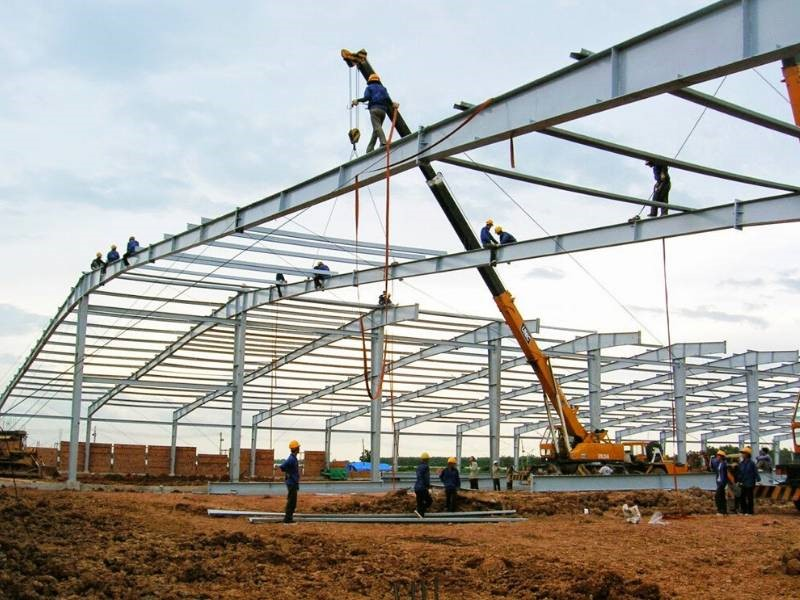
\includegraphics[width=186mm]{../../public/about1.jpg}};
  \fill[TTCDeepNavy, opacity=0.86] (0,0) rectangle (68,64);
  \fill[TTCDeepNavy, opacity=0.28] (68,0) rectangle (92,64);
  \node[anchor=west, text width=54mm, align=left, text=white] at (8,42) {
    {\fontsize{7}{8}\selectfont\bfseries\color{TTCCyan} STRATEGIC PEB NETWORK}\\[1.3mm]
    {\fontsize{18}{20}\selectfont\bfseries PLANNING}\\[-0.4mm]
    {\fontsize{8}{9.5}\selectfont\bfseries\color{TTCCyan} PROFILE ACCORDING TO THE PROJECT PACKAGE}\\[1.8mm]
    {\fontsize{7}{8.6}\selectfont\color{white!82!gray}
    TTC owns the design, Shop Drawing and factory approval rights.}
  };
  \node[
    anchor=south east, rounded corners=3pt,
    fill=white, fill opacity=0.94, text opacity=1,
    draw=TTCCyan, line width=0.65pt,
    minimum width=55mm, minimum height=14mm, align=center
  ] at (179,7) {
    {\fontsize{9.5}{11}\selectfont\bfseries\color{TTCBlue} PARTNER FACTORY • RESIDENT QC}\\[0.6mm]
    {\fontsize{6.5}{7.8}\selectfont\color{TTCTextDark}Approved production plan • TTC supervision}
  };
  \draw[white, line width=1pt, rounded corners=3pt] (0.6,0.6) rectangle (185.4,63.4);
  \draw[TTCBorder, line width=0.65pt, rounded corners=3pt] (0,0) rectangle (186,64);
\end{tikzpicture}

\vspace{3mm}

% SIX-STAGE FABRICATION FLOW
\noindent
\begin{tikzpicture}[x=1mm,y=1mm]
  \path[use as bounding box] (0,0) rectangle (186,53);
  \node[anchor=west] at (0,48) {
    {\fontsize{7}{8}\selectfont\bfseries\color{TTCCyan} FABRICATION FLOW}\quad
    {\fontsize{9.5}{11}\selectfont\bfseries\color{TTCBlue} SIX CLOSED MACHINING STAGES}
  };
  \draw[TTCBlue!30!white, line width=0.85pt] (15,31) -- (171,31);

  \foreach \x/\num in {15/01,46/02,77/03,108/04,139/05,171/06}{
    \fill[white] (\x,31) circle (4.8);
    \draw[TTCBlue!48!white, line width=0.75pt] (\x,31) circle (4.8);
    \node[text=TTCBlue, font=\fontsize{6.8}{8}\selectfont\bfseries] at (\x,31) {\num};
  }
  \fill[TTCRed] (171,31) circle (4.8);
  \node[text=white, font=\fontsize{6.8}{8}\selectfont\bfseries] at (171,31) {06};

  \node[align=center, text width=25mm] at (15,13) {
    {\fontsize{8}{9.2}\selectfont\bfseries\color{TTCBlue} CNC CUTTING}\\[0.6mm]
    {\fontsize{6.3}{7.5}\selectfont Plasma • bevel}
  };
  \node[align=center, text width=25mm] at (46,13) {
    {\fontsize{8}{9.2}\selectfont\bfseries\color{TTCBlue} FIT-UP}\\[0.6mm]
    {\fontsize{6.3}{7.5}\selectfont Hydraulic jig}
  };
  \node[align=center, text width=25mm] at (77,13) {
    {\fontsize{8}{9.2}\selectfont\bfseries\color{TTCBlue} SAW WELD}\\[0.6mm]
    {\fontsize{6.3}{7.5}\selectfont AWS D1.1}
  };
  \node[align=center, text width=25mm] at (108,13) {
    {\fontsize{8}{9.2}\selectfont\bfseries\color{TTCBlue} STRAIGHTEN}\\[0.6mm]
    {\fontsize{6.3}{7.5}\selectfont Hydraulic press}
  };
  \node[align=center, text width=25mm] at (139,13) {
    {\fontsize{8}{9.2}\selectfont\bfseries\color{TTCBlue} BLASTING}\\[0.6mm]
    {\fontsize{6.3}{7.5}\selectfont Sa 2.5}
  };
  \node[align=center, text width=25mm] at (171,13) {
    {\fontsize{8}{9.2}\selectfont\bfseries\color{TTCRed} COATING}\\[0.6mm]
    {\fontsize{6.3}{7.5}\selectfont Epoxy • fireproof}
  };
\end{tikzpicture}

\vspace{3mm}

% QUALITY GATES
\noindent
\begin{tikzpicture}[x=1mm,y=1mm]
  \path[use as bounding box] (0,0) rectangle (186,53);

  \fill[white, rounded corners=4pt] (0,0) rectangle (58,53);
  \draw[TTCBorder, line width=0.65pt, rounded corners=4pt] (0,0) rectangle (58,53);
  \node[anchor=north west, text width=48mm, align=left] at (5,47) {
    {\fontsize{7}{8}\selectfont\bfseries\color{TTCCyan} QUALITY GATE 01}\\[0.8mm]
    {\fontsize{10}{11.5}\selectfont\bfseries\color{TTCBlue} MATERIAL RELEASE}\\[1.3mm]
    {\fontsize{7}{8.5}\selectfont\color{TTCTextDark}
    \textcolor{TTCCyan}{\faCheckCircle}\ MTC, CO/CQ and steel lot retrieval.\\[0.7mm]
    \textcolor{TTCCyan}{\faCheckCircle}\ Q345B • SS400 • ASTM A572 Gr.50.\\[0.7mm]
    \textcolor{TTCCyan}{\faCheckCircle}\ Independent mechanical and physical tests.}
  };

  \fill[TTCLightBlue, rounded corners=4pt] (64,0) rectangle (122,53);
  \draw[TTCBlue!50!white, line width=0.7pt, rounded corners=4pt] (64,0) rectangle (122,53);
  \node[anchor=north west, text width=48mm, align=left] at (69,47) {
    {\fontsize{7}{8}\selectfont\bfseries\color{TTCCyan} QUALITY GATE 02}\\[0.8mm]
    {\fontsize{10}{11.5}\selectfont\bfseries\color{TTCBlue} WELD ACCEPTANCE}\\[1.3mm]
    {\fontsize{7}{8.5}\selectfont\color{TTCTextDark}
    \textcolor{TTCBlue}{\faCheckCircle}\ WPS/PQR approved.\\[0.7mm]
    \textcolor{TTCBlue}{\faCheckCircle}\ Welders with 3G/4G/6G certificates.\\[0.7mm]
    \textcolor{TTCBlue}{\faCheckCircle}\ NDT UT/MT load-bearing weld joints.}
  };

  \fill[white, rounded corners=4pt] (128,0) rectangle (186,53);
  \draw[TTCRed!65!white, line width=0.75pt, rounded corners=4pt] (128,0) rectangle (186,53);
  \node[anchor=north west, text width=48mm, align=left] at (133,47) {
    {\fontsize{7}{8}\selectfont\bfseries\color{TTCRed} QUALITY GATE 03}\\[0.8mm]
    {\fontsize{10}{11.5}\selectfont\bfseries\color{TTCBlue} FINISH \& RELEASE}\\[1.3mm]
    {\fontsize{7}{8.5}\selectfont\color{TTCTextDark}
    \textcolor{TTCRed}{\faCheckCircle}\ Clean Sa 2.5 according to ISO 8501-1.\\[0.7mm]
    \textcolor{TTCRed}{\faCheckCircle}\ DFT by Elcometer.\\[0.7mm]
    \textcolor{TTCRed}{\faCheckCircle}\ Epoxy paint and fire prevention and fighting.}
  };
\end{tikzpicture}

\vspace{3mm}

% TTC RELEASE AUTHORITY
\noindent
\begin{tikzpicture}[x=1mm,y=1mm]
  \path[use as bounding box] (0,0) rectangle (186,30);
  \fill[TTCLightBlue, rounded corners=4pt] (0,0) rectangle (186,30);
  \draw[TTCBorder, line width=0.65pt, rounded corners=4pt] (0,0) rectangle (186,30);
  \node[anchor=west, align=left] at (6,15) {
    {\fontsize{7}{8}\selectfont\bfseries\color{TTCCyan} TTC CONTROL MODEL}\\[0.7mm]
    {\fontsize{9.3}{10.8}\selectfont\bfseries\color{TTCBlue} PERMISSION TO APPROVE FACTORY RELEASE}
  };
  \node[text=TTCRed] at (55,15) {\faChevronRight};
  \node[align=center] at (76,15) {
    {\fontsize{8.5}{10}\selectfont\bfseries\color{TTCBlue} DESIGN \& SHOP}\\[0.5mm]
    {\fontsize{6.3}{7.5}\selectfont TTC engineering}
  };
  \node[text=TTCRed] at (97,15) {\faChevronRight};
  \node[align=center] at (117,15) {
    {\fontsize{8.5}{10}\selectfont\bfseries\color{TTCBlue} RESIDENT QC}\\[0.5mm]
    {\fontsize{6.3}{7.5}\selectfont At partner factory}
  };
  \node[text=TTCRed] at (137,15) {\faChevronRight};
  \node[align=center] at (158,15) {
    {\fontsize{8.5}{10}\selectfont\bfseries\color{TTCRed} RELEASE NOTE}\\[0.5mm]
    {\fontsize{6.3}{7.5}\selectfont Ready for erection}
  };
\end{tikzpicture}
\vfill
\noindent\makebox[\linewidth][c]{%
  \begin{tikzpicture}[x=1mm,y=1mm]
    \path[use as bounding box] (0,0) rectangle (210,9);
    \begin{scope}[yshift=-20mm]
    \fill[TTCDeepNavy] (0,0) rectangle (210,8);
    \fill[TTCCyan] (0,8) rectangle (210,9);
    \node[anchor=west, text=white, font=\fontsize{6.8}{8}\selectfont]
      at (12,4) {\faPhone*\ +84 976 447 766 \quad\textbullet\quad \faEnvelope\ info@tanthanhcongjsc.com \quad\textbullet\quad \faGlobe\ https://tanthanhcongjsc.com};
    \node[anchor=east, text=white, font=\fontsize{7}{8}\selectfont\bfseries]
      at (198,4) {Page 11};
    \end{scope}
  \end{tikzpicture}%
}
\end{minipage}
\newpage

% ============================================================
% PAGE 12: THIẾT BỊ THEO GÓI HUY ĐỘNG
% ============================================================
\pageheaderbar{CONSTRUCTION EQUIPMENT \& SITE MOBILIZATION}{Page 12}
\pagefooterbar{Page 12}

\begin{tikzpicture}[remember picture, overlay]
  \fill[TTCLightBlue]
    ([xshift=137mm,yshift=-31mm]current page.north west) --
    ([xshift=210mm,yshift=-31mm]current page.north west) --
    ([xshift=210mm,yshift=-104mm]current page.north west) -- cycle;
  \draw[TTCBlue!8!white, line width=12pt]
    ([xshift=151mm,yshift=42mm]current page.south west) --
    ([xshift=205mm,yshift=96mm]current page.south west);
  \draw[TTCRed!8!white, line width=3pt]
    ([xshift=160mm,yshift=42mm]current page.south west) --
    ([xshift=205mm,yshift=87mm]current page.south west);
  % Faint industrial mobilization silhouette — replaces the old square grid
  \begin{scope}[shift={(current page.south west)},x=1mm,y=1mm,opacity=.48]
    \draw[TTCBlue!18!white, line width=.7pt] (12,13) -- (198,13);
    \fill[TTCBlue!2!white] (14,13) -- (14,34) -- (34,43) -- (54,34) --
      (54,13) -- cycle;
    \draw[TTCBlue!17!white, line width=.65pt] (14,13) -- (14,34) -- (34,43) --
      (54,34) -- (54,13);
    \foreach \x in {19,27,35,43,51}{\draw[TTCBlue!13!white] (\x,13) -- (\x,34);}
    \fill[TTCBlue!2!white] (61,13) rectangle (133,31);
    \draw[TTCBlue!17!white, line width=.65pt] (61,13) rectangle (133,31);
    \foreach \x in {73,85,97,109,121}{\draw[TTCBlue!12!white] (\x,13) -- (\x,31);}
    \draw[TTCBlue!17!white] (61,22) -- (133,22);
    % tower crane / lifting cue
    \draw[TTCBlue!20!white, line width=.85pt] (151,13) -- (151,51);
    \draw[TTCBlue!18!white] (146,13) -- (151,51) -- (156,13);
    \draw[TTCBlue!20!white, line width=.85pt] (151,48) -- (198,48);
    \draw[TTCBlue!17!white] (151,48) -- (177,39) -- (198,48);
    \draw[TTCRed!22!white, line width=.7pt] (184,48) -- (184,25);
    \draw[TTCRed!22!white] (181,25) -- (187,25);
  \end{scope}
\end{tikzpicture}

\begin{minipage}[t][246mm]{\textwidth}
\secbrand{Equipment Capacity by Mobilization Package}{Right Equipment, Right Workfront, Right Time}

{\fontsize{15}{17}\selectfont\bfseries\color{TTCBlue}
43+ EQUIPMENT • 4 MISSION PACKAGES • COORDINATED BY ONE CONTRACT\par}
\vspace{1mm}
{\fontsize{7.5}{9}\selectfont\color{TTCTextMuted}
The list is streamlined according to execution capacity, prioritizing maneuverability, accreditation and performance on site.\par}
\vspace{3mm}

% HERO — SITE MOBILIZATION
\noindent
\begin{tikzpicture}[x=1mm,y=1mm]
  \path[use as bounding box] (0,0) rectangle (186,58);
  \clip[rounded corners=3pt] (0,0) rectangle (186,58);
  \node[anchor=center, inner sep=0pt] at (93,29)
    {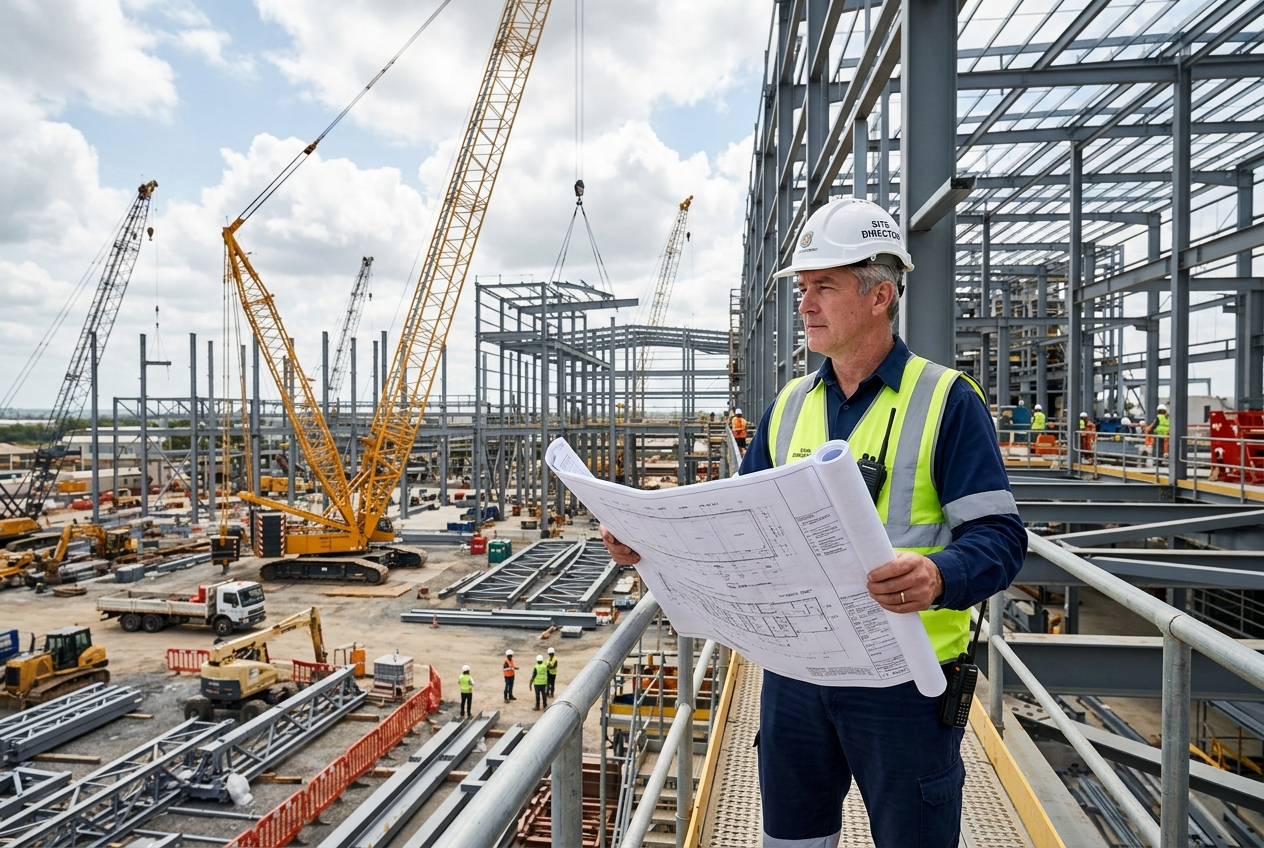
\includegraphics[width=186mm]{../../public/c_level_site_inspection.jpg}};
  \fill[TTCDeepNavy, opacity=0.88] (0,0) rectangle (68,58);
  \fill[TTCDeepNavy, opacity=0.35] (68,0) rectangle (94,58);
  \node[anchor=west, text width=54mm, align=left, text=white] at (8,38) {
    {\fontsize{7}{8}\selectfont\bfseries\color{TTCCyan} MOBILIZATION CONTROL}\\[1.5mm]
    {\fontsize{21}{22}\selectfont\bfseries 43+}\\[-0.5mm]
    {\fontsize{9}{10.5}\selectfont\bfseries READY EQUIPMENT}\\[1.7mm]
    {\fontsize{7}{8.5}\selectfont\color{white!82!gray}
    Coordinate according to the critical path and construction site, do not spread resources.}
  };
  \node[rounded corners=2pt, fill=white, text=TTCBlue, align=center,
        minimum width=31mm, minimum height=16mm] at (129,17) {
    {\fontsize{13}{14}\selectfont\bfseries 100T}\\[-0.4mm]
    {\fontsize{6.2}{7.4}\selectfont MAXIMUM LIFTING CAPACITY}
  };
  \node[rounded corners=2pt, fill=TTCRed, text=white, align=center,
        minimum width=35mm, minimum height=16mm] at (167,17) {
    {\fontsize{11}{12}\selectfont\bfseries VALID}\\[-0.4mm]
    {\fontsize{6.2}{7.4}\selectfont COMPANY ACCREDITATION}
  };
\end{tikzpicture}

\vspace{3mm}

% FOUR MISSION PACKAGES
\noindent
\begin{tikzpicture}[x=1mm,y=1mm]
  \path[use as bounding box] (0,0) rectangle (186,50);
  \foreach \x/\accent in {0/TTCRed,47.5/TTCCyan,95/TTCBlue,142.5/TTCGold}{
    \fill[white, rounded corners=2pt] (\x,0) rectangle +(43.5,50);
    \draw[TTCBorder, rounded corners=2pt, line width=.55pt] (\x,0) rectangle +(43.5,50);
    \fill[\accent, rounded corners=2pt] (\x,46) rectangle +(43.5,4);
  }
  \node[anchor=north west, text width=35mm, align=left] at (4,43) {
    {\fontsize{15}{16}\selectfont\bfseries\color{TTCRed} 20}\\[-.5mm]
    {\fontsize{7.4}{8.5}\selectfont\bfseries\color{TTCBlue} LOWER \& OUTREACH}\\[1mm]
    {\fontsize{6.6}{8}\selectfont\color{TTCTextDark}
    06 self-propelled cranes 25--100T\newline
    14 xe Boomlift 18--28m\newline
    Erection of steel, roof and MEP at height.}
  };
  \node[anchor=north west, text width=35mm, align=left] at (51.5,43) {
    {\fontsize{15}{16}\selectfont\bfseries\color{TTCCyan} 12}\\[-.5mm]
    {\fontsize{7.4}{8.5}\selectfont\bfseries\color{TTCBlue} BACKGROUND \& CONCRETE}\\[1mm]
    {\fontsize{6.6}{8}\selectfont\color{TTCTextDark}
    08 excavators, road roller\newline
    04 concrete pumps and tanks\newline
    Infrastructure, foundations and industrial floors.}
  };
  \node[anchor=north west, text width=35mm, align=left] at (99,43) {
    {\fontsize{15}{16}\selectfont\bfseries\color{TTCBlue} 02}\\[-.5mm]
    {\fontsize{7.4}{8.5}\selectfont\bfseries\color{TTCBlue} ROOF \& BAO CHE}\\[1mm]
    {\fontsize{6.6}{8}\selectfont\color{TTCTextDark}
    02 movable coils\newline
    Cliplock / Seamlock in place\newline
    Long strip of corrugated iron, limiting joints and seepage.}
  };
  \node[anchor=north west, text width=35mm, align=left] at (146.5,43) {
    {\fontsize{15}{16}\selectfont\bfseries\color{TTCGold} 09}\\[-.5mm]
    {\fontsize{7.4}{8.5}\selectfont\bfseries\color{TTCBlue} SURVEYING \& QA}\\[1mm]
    {\fontsize{6.6}{8}\selectfont\color{TTCTextDark}
    09 sets of Leica / Laser 3D\newline
    Axial heart and pitch control\newline
    Target error less than 2mm.}
  };
\end{tikzpicture}

\vspace{3mm}

% DEPLOYMENT SEQUENCE
\noindent
\begin{tikzpicture}[x=1mm,y=1mm]
  \path[use as bounding box] (0,0) rectangle (186,42);
  \fill[TTCLightBlue, rounded corners=3pt] (0,0) rectangle (186,42);
  \draw[TTCBorder, rounded corners=3pt, line width=.6pt] (0,0) rectangle (186,42);
  \node[anchor=west, font=\fontsize{8}{9.5}\selectfont\bfseries, text=TTCBlue] at (7,35)
    {\faClock\quad PROJECT CRITICAL PATH MOBILIZATION RHYTHM};
  \draw[TTCBlue!35!white, line width=1pt] (19,19) -- (167,19);
  \foreach \x/\n/\t/\s in {
    21/01/FOUNDATION/Survey • earthwork • concrete,
    69/02/STRUCTURE/Crane installation • overhead access,
    117/03/COVER/Rolled • roof • finish,
    165/04/ACCEPTANCE/surveying • inspection • handover}{
      \fill[white] (\x,19) circle (4.7);
      \draw[TTCBlue, line width=.8pt] (\x,19) circle (4.7);
      \node[font=\fontsize{6.8}{8}\selectfont\bfseries, text=TTCRed] at (\x,19) {\n};
      \node[anchor=north, align=center, text width=38mm] at (\x,12) {
        {\fontsize{6.8}{8}\selectfont\bfseries\color{TTCBlue} \t}\\[-.3mm]
        {\fontsize{5.8}{7}\selectfont\color{TTCTextMuted} \s}
      };
  }
\end{tikzpicture}

\vspace{3mm}

% ASSURANCE STRIP
\noindent
\begin{tikzpicture}[x=1mm,y=1mm]
  \path[use as bounding box] (0,0) rectangle (186,29);
  \fill[TTCDeepNavy, rounded corners=3pt] (0,0) rectangle (186,29);
  \foreach \x in {46.5,93,139.5}{\draw[white!35!gray] (\x,6) -- (\x,23);}
  \node[align=center, text=white] at (23.25,15) {{\fontsize{9}{10}\selectfont\bfseries\color{TTCRed} PLANNED}\\[-.3mm]{\fontsize{6.2}{7.4}\selectfont Glove Line Maneuvering}};
  \node[align=center, text=white] at (69.75,15) {{\fontsize{9}{10}\selectfont\bfseries\color{TTCCyan} CERTIFICATE}\\[-.3mm]{\fontsize{6.2}{7.4}\selectfont Proper Operation}};
  \node[align=center, text=white] at (116.25,15) {{\fontsize{9}{10}\selectfont\bfseries MAINTENANCE}\\[-.3mm]{\fontsize{6.2}{7.4}\selectfont According to the Firm Recommendations}};
  \node[align=center, text=white] at (162.75,15) {{\fontsize{9}{10}\selectfont\bfseries\color{TTCGold} JOURNAL NO.}\\[-.3mm]{\fontsize{6.2}{7.4}\selectfont Time-Based Status}};
\end{tikzpicture}
\end{minipage}
\newpage

% ============================================================
% PAGE 13: QUẢN TRỊ DỰ ÁN STAGE-GATE
% ============================================================
\pagefooterbar{Page 13}

\begin{tikzpicture}[remember picture, overlay]
  \fill[TTCLightBlue]
    ([xshift=118mm,yshift=-32mm]current page.north west) --
    ([xshift=210mm,yshift=-32mm]current page.north west) --
    ([xshift=210mm,yshift=-118mm]current page.north west) -- cycle;
  \node[opacity=.035, font=\fontsize{62}{64}\selectfont\bfseries, text=TTCBlue,
        rotate=90] at ([xshift=-10mm,yshift=18mm]current page.east) {GATE};
  % Four translucent decision chevrons continue the process into the footer
  \begin{scope}[shift={(current page.south west)},x=1mm,y=1mm,opacity=.42]
    \foreach \x/\c in {15/TTCRed,60/TTCCyan,105/TTCBlue,150/TTCGold}{
      \fill[\c!7!white] (\x,14) -- ++(31,0) -- ++(10,14) -- ++(-10,14) --
        ++(-31,0) -- ++(10,-14) -- cycle;
    }
    \node[text=TTCRed!35!white,font=\fontsize{7}{8}\selectfont\bfseries] at (35,28) {DEFINE};
    \node[text=TTCCyan!40!white,font=\fontsize{7}{8}\selectfont\bfseries] at (80,28) {ENGINEER};
    \node[text=TTCBlue!35!white,font=\fontsize{7}{8}\selectfont\bfseries] at (125,28) {BUILD};
    \node[text=TTCGold!40!white,font=\fontsize{7}{8}\selectfont\bfseries] at (170,28) {HANDOVER};
  \end{scope}
\end{tikzpicture}

\begin{minipage}[t][246mm]{\textwidth}
\pageheaderbar{STAGE-GATE EPC PROJECT GOVERNANCE}{Page 13}
\secbrand{EPC Governance Through Four Control Phases}{FIDIC Turnkey Governance, Decision Gates \& Single-Point Accountability}

{\fontsize{15}{17}\selectfont\bfseries\color{TTCBlue}
EACH PHASE WITH OUTPUT • EACH PHASE TRANSITION WITH APPROVAL\par}
\vspace{1mm}
{\fontsize{7.5}{9}\selectfont\color{TTCTextMuted}
The eight steps of implementation are grouped into four governance phases, helping Client to clearly see the decision, responsibility and status of the project.\par}
\vspace{3mm}

% FOUR PHASES / FOUR GATES
\noindent
\begin{tikzpicture}[x=1mm,y=1mm]
  \path[use as bounding box] (0,0) rectangle (186,103);

  % PHASE 01
  \fill[white, rounded corners=2pt] (0,0) rectangle (43.5,103);
  \draw[TTCBorder, rounded corners=2pt, line width=.65pt] (0,0) rectangle (43.5,103);
  \fill[TTCDeepNavy, rounded corners=2pt] (0,84) rectangle (43.5,103);
  \node[anchor=west, text=white] at (4,94) {{\fontsize{7}{8}\selectfont 01}\quad{\fontsize{10}{11}\selectfont\bfseries DEFINE}};
  \node[anchor=north west, text width=35.5mm, align=left] at (4,79) {
    {\fontsize{7}{8.5}\selectfont\bfseries\color{TTCRed} 01 • SURVEY \& BRIEF}\\[.7mm]
    {\fontsize{6.2}{7.5}\selectfont\color{TTCTextDark}Geology, 3D topography; performance requirements and pre-feasibility report.}\\[3mm]
    {\fontsize{7}{8.5}\selectfont\bfseries\color{TTCBlue} 02 • LEGAL \& PLANNING}\\[.7mm]
    {\fontsize{6.2}{7.5}\selectfont\color{TTCTextDark}Planning 1/500, EIA, fire prevention and fighting, construction permits and design facilities.}
  };
  \fill[TTCRed!8!white] (3.5,5) rectangle (40,17);
  \node[align=center, text=TTCRed] at (21.75,11) {{\fontsize{6}{7}\selectfont\bfseries GATE A}\\[-.2mm]{\fontsize{5.7}{6.7}\selectfont Basis Approved}};

  % PHASE 02
  \fill[white, rounded corners=2pt] (47.5,0) rectangle (91,103);
  \draw[TTCBorder, rounded corners=2pt, line width=.65pt] (47.5,0) rectangle (91,103);
  \fill[TTCBlue, rounded corners=2pt] (47.5,84) rectangle (91,103);
  \node[anchor=west, text=white] at (51.5,94) {{\fontsize{7}{8}\selectfont 02}\quad{\fontsize{10}{11}\selectfont\bfseries ENGINEER}};
  \node[anchor=north west, text width=35.5mm, align=left] at (51.5,79) {
    {\fontsize{7}{8.5}\selectfont\bfseries\color{TTCCyan} 03 • VALUE ENGINEERING}\\[.7mm]
    {\fontsize{6.2}{7.5}\selectfont\color{TTCTextDark}BIM LOD 400, structure optimization, subject coordination and conflict control.}\\[3mm]
    {\fontsize{7}{8.5}\selectfont\bfseries\color{TTCBlue} 04 • PROCUREMENT \& PEB}\\[.7mm]
    {\fontsize{6.2}{7.5}\selectfont\color{TTCTextDark}Tier-1 supplies, Shop Drawing, procurement plan and permanent QC at the workshop.}
  };
  \fill[TTCCyan!10!white] (51,5) rectangle (87.5,17);
  \node[align=center, text=TTCBlue] at (69.25,11) {{\fontsize{6}{7}\selectfont\bfseries GATE B}\\[-.2mm]{\fontsize{5.7}{6.7}\selectfont Design Freeze}};

  % PHASE 03
  \fill[white, rounded corners=2pt] (95,0) rectangle (138.5,103);
  \draw[TTCBorder, rounded corners=2pt, line width=.65pt] (95,0) rectangle (138.5,103);
  \fill[TTCCyan!85!TTCBlue, rounded corners=2pt] (95,84) rectangle (138.5,103);
  \node[anchor=west, text=white] at (99,94) {{\fontsize{7}{8}\selectfont 03}\quad{\fontsize{10}{11}\selectfont\bfseries BUILD}};
  \node[anchor=north west, text width=35.5mm, align=left] at (99,79) {
    {\fontsize{7}{8.5}\selectfont\bfseries\color{TTCRed} 05 • GROUND \& INFRA}\\[.7mm]
    {\fontsize{6.2}{7.5}\selectfont\color{TTCTextDark}Piles, foundations, foundations, technical infrastructure and workfronts handover according to ITP.}\\[3mm]
    {\fontsize{7}{8.5}\selectfont\bfseries\color{TTCBlue} 06 • STRUCTURE \& MEP}\\[.7mm]
    {\fontsize{6.2}{7.5}\selectfont\color{TTCTextDark}Steel structure, cover, MEP, fire prevention and fighting and control of schedule critical path.}
  };
  \fill[TTCBlue!8!white] (98.5,5) rectangle (135,17);
  \node[align=center, text=TTCBlue] at (116.75,11) {{\fontsize{6}{7}\selectfont\bfseries GATE C}\\[-.2mm]{\fontsize{5.7}{6.7}\selectfont Ready To Test}};

  % PHASE 04
  \fill[white, rounded corners=2pt] (142.5,0) rectangle (186,103);
  \draw[TTCBorder, rounded corners=2pt, line width=.65pt] (142.5,0) rectangle (186,103);
  \fill[TTCGold, rounded corners=2pt] (142.5,84) rectangle (186,103);
  \node[anchor=west, text=white] at (146.5,94) {{\fontsize{7}{8}\selectfont 04}\quad{\fontsize{10}{11}\selectfont\bfseries HANDOVER}};
  \node[anchor=north west, text width=35.5mm, align=left] at (146.5,79) {
    {\fontsize{7}{8.5}\selectfont\bfseries\color{TTCRed} 07 • TEST \& APPROVAL}\\[.7mm]
    {\fontsize{6.2}{7.5}\selectfont\color{TTCTextDark}Acceptance of ITP, fire prevention and fighting, single-motor test run and system interconnection.}\\[3mm]
    {\fontsize{7}{8.5}\selectfont\bfseries\color{TTCBlue} 08 • HANDOVER \& O\&M}\\[.7mm]
    {\fontsize{6.2}{7.5}\selectfont\color{TTCTextDark}As-built, Digital Twin, operation training, warranty and maintenance plan.}
  };
  \fill[TTCGold!12!white] (146,5) rectangle (182.5,17);
  \node[align=center, text=TTCGold!80!black] at (164.25,11) {{\fontsize{6}{7}\selectfont\bfseries GATE D}\\[-.2mm]{\fontsize{5.7}{6.7}\selectfont Ready To Operate}};

  % TRANSITION MARKERS
  \foreach \x/\l in {45.5/A,93/B,140.5/C}{
    \fill[white] (\x,51) circle (3.8);
    \draw[TTCRed, line width=.8pt] (\x,51) circle (3.8);
    \node[text=TTCRed, font=\fontsize{5.5}{6}\selectfont\bfseries] at (\x,51) {\l};
  }
\end{tikzpicture}

\vspace{3mm}

% GOVERNANCE SPINE
\noindent
\begin{tikzpicture}[x=1mm,y=1mm]
  \path[use as bounding box] (0,0) rectangle (186,43);
  \fill[TTCLightBlue, rounded corners=3pt] (0,0) rectangle (186,43);
  \draw[TTCBorder, rounded corners=3pt, line width=.6pt] (0,0) rectangle (186,43);
  \node[anchor=west, text=TTCBlue, font=\fontsize{8}{9.5}\selectfont\bfseries] at (7,35)
    {\faProjectDiagram\quad GOVERNANCE SPINE — A GOVERNANCE SYSTEM THROUGHOUT};
  \foreach \x in {46.5,93,139.5}{\draw[TTCBorder] (\x,6) -- (\x,28);}
  \node[align=center, text width=39mm] at (23.25,17) {{\fontsize{7}{8}\selectfont\bfseries\color{TTCRed} PROJECT DIRECTOR}\\[-.2mm]{\fontsize{5.8}{7}\selectfont\color{TTCTextMuted}A focal point responsible for the output}};
  \node[align=center, text width=39mm] at (69.75,17) {{\fontsize{7}{8}\selectfont\bfseries\color{TTCBlue} CPM BASELINE}\\[-.2mm]{\fontsize{5.8}{7}\selectfont\color{TTCTextMuted}Weekly glove and look-ahead lines}};
  \node[align=center, text width=39mm] at (116.25,17) {{\fontsize{7}{8}\selectfont\bfseries\color{TTCCyan} COMMON DATA ENV.}\\[-.2mm]{\fontsize{5.8}{7}\selectfont\color{TTCTextMuted}Traceable Drawings, RFI, ITP}};
  \node[align=center, text width=39mm] at (162.75,17) {{\fontsize{7}{8}\selectfont\bfseries\color{TTCGold} FIDIC CONTROL}\\[-.2mm]{\fontsize{5.8}{7}\selectfont\color{TTCTextMuted}Scope, change and contract risk}};
\end{tikzpicture}

\vspace{3mm}

% OUTCOME STRIP
\noindent
\begin{tikzpicture}[x=1mm,y=1mm]
  \path[use as bounding box] (0,0) rectangle (186,29);
  \fill[TTCDeepNavy, rounded corners=3pt] (0,0) rectangle (186,29);
  \foreach \x in {46.5,93,139.5}{\draw[white!35!gray] (\x,6) -- (\x,23);}
  \node[align=center, text=white] at (23.25,15) {{\fontsize{9}{10}\selectfont\bfseries\color{TTCRed} 8 STEPS}\\[-.3mm]{\fontsize{6.2}{7.4}\selectfont In 4 Control Phases}};
  \node[align=center, text=white] at (69.75,15) {{\fontsize{9}{10}\selectfont\bfseries\color{TTCCyan} 4 GATES}\\[-.3mm]{\fontsize{6.2}{7.4}\selectfont Conditional Determination}};
  \node[align=center, text=white] at (116.25,15) {{\fontsize{9}{10}\selectfont\bfseries FIDIC EPC}\\[-.3mm]{\fontsize{6.2}{7.4}\selectfont International Contract Standard}};
  \node[align=center, text=white] at (162.75,15) {{\fontsize{9}{10}\selectfont\bfseries\color{TTCGold} CONTRACTUAL}\\[-.3mm]{\fontsize{6.2}{7.4}\selectfont Warranty and After Sales}};
\end{tikzpicture}
\end{minipage}
\newpage

% ============================================================
% PAGE 14: EPC VALUE MODEL — ONE CONTRACT, ONE ACCOUNTABILITY
% ============================================================
\begin{tikzpicture}[remember picture, overlay]
  \fill[TTCLightBlue]
    ([xshift=132mm,yshift=-30mm]current page.north west) --
    ([xshift=210mm,yshift=-30mm]current page.north west) --
    ([xshift=210mm,yshift=-104mm]current page.north west) -- cycle;
  \draw[TTCBlue!7!white, line width=12pt]
    ([xshift=154mm,yshift=37mm]current page.south west) --
    ([xshift=205mm,yshift=88mm]current page.south west);
  \draw[TTCRed!8!white, line width=3pt]
    ([xshift=162mm,yshift=37mm]current page.south west) --
    ([xshift=205mm,yshift=80mm]current page.south west);
  % A light structural frame at the bottom — no square grid
  \begin{scope}[shift={(current page.south west)},x=1mm,y=1mm,opacity=.42]
    \draw[TTCBlue!17!white, line width=.7pt] (12,13) -- (198,13);
    \draw[TTCBlue!16!white] (17,13) -- (17,37) -- (47,50) -- (77,37) --
      (107,50) -- (137,37) -- (167,50) -- (197,37) -- (197,13);
    \foreach \x in {17,47,77,107,137,167,197}{\draw[TTCBlue!12!white] (\x,13) -- (\x,42);}
    \draw[TTCRed!18!white, line width=.7pt] (17,20) -- (197,20);
  \end{scope}
\end{tikzpicture}

\pagefooterbar{Page 14}
\begin{minipage}[t][246mm]{\textwidth}
\pageheaderbar{EPC DELIVERY \& VALUE ENGINEERING}{Page 14}
\vspace{6mm}
\secbrand{Value-Creating EPC Delivery Model}{Fast-Track Delivery, Value Engineering \& Single-Point Accountability}

{\fontsize{15}{17}\selectfont\bfseries\color{TTCBlue}
FASTER • LEANER • LESS RISKY\par}
\vspace{1mm}
{\fontsize{7.5}{9}\selectfont\color{TTCTextMuted}
TTC integrates legal, design, procurement and construction in one contract — all decisions together towards the final investment efficiency.\par}
\vspace{3mm}

% HERO — THE FACILITY AS ONE INTEGRATED SYSTEM
\noindent
\begin{tikzpicture}[x=1mm,y=1mm]
  \path[use as bounding box] (0,0) rectangle (186,66);
  \clip[rounded corners=3pt] (0,0) rectangle (186,66);
  \node[anchor=center, inner sep=0pt] at (93,33)
    {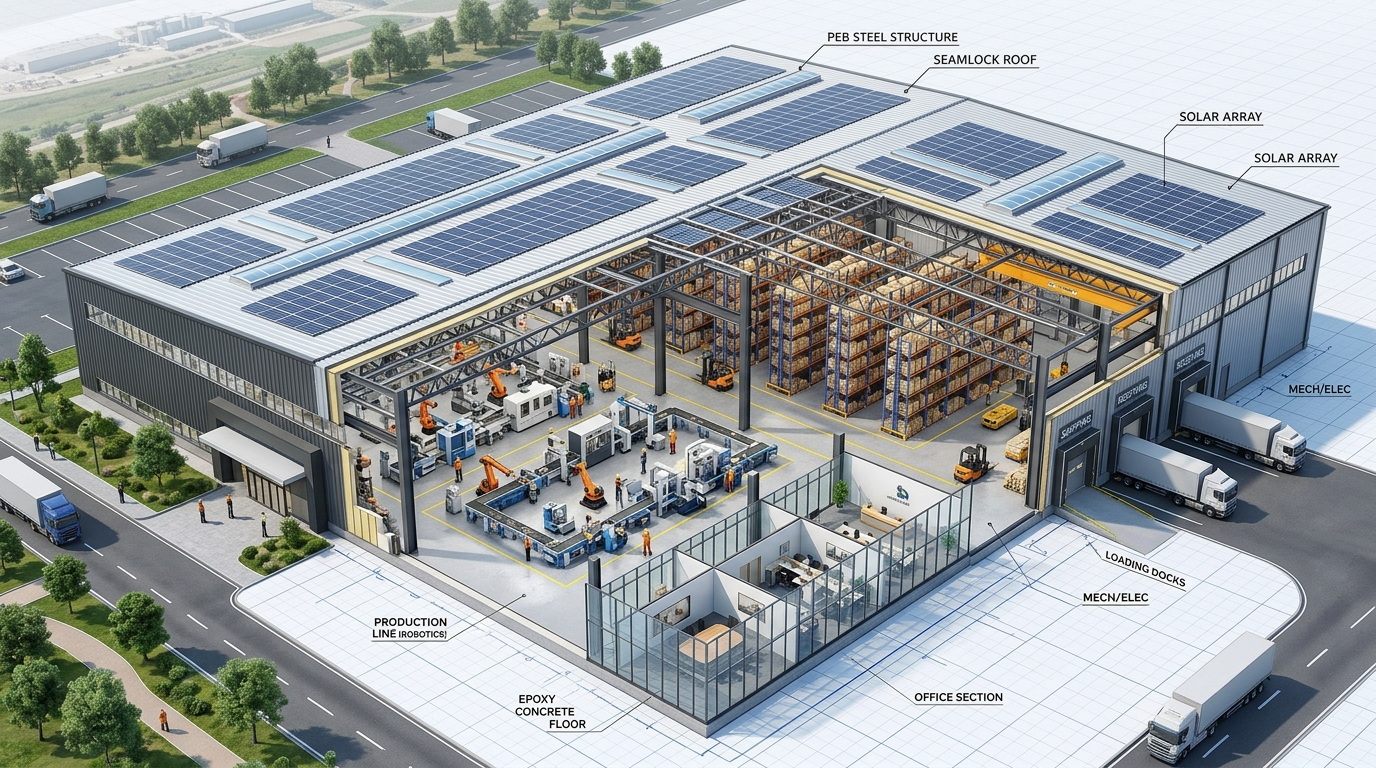
\includegraphics[width=186mm]{../../public/factory-tech-3d.jpg}};
  \fill[TTCDeepNavy, opacity=.88] (0,0) rectangle (66,66);
  \fill[TTCDeepNavy, opacity=.26] (66,0) rectangle (92,66);
  \node[anchor=west, text width=52mm, align=left, text=white] at (8,43) {
    {\fontsize{7}{8}\selectfont\bfseries\color{TTCCyan} TTC EPC VALUE MODEL}\\[1.3mm]
    {\fontsize{17}{19}\selectfont\bfseries ONE CONTRACT}\\[-.2mm]
    {\fontsize{10}{12}\selectfont\bfseries\color{TTCRed!85!white} ONE ACCOUNTABILITY}\\[1.7mm]
    {\fontsize{7}{8.5}\selectfont\color{white!82!gray}
    A focal point controlling scope, budget, schedule and quality handover.}
  };
  \node[rounded corners=2pt, fill=white, align=center, minimum width=29mm,
        minimum height=15mm] at (113,15) {
    {\fontsize{9}{10}\selectfont\bfseries\color{TTCRed} REVIEWED}\\[-.3mm]
    {\fontsize{5.8}{7}\selectfont\color{TTCBlue} STRUCTURAL OPTION}
  };
  \node[rounded corners=2pt, fill=white, align=center, minimum width=29mm,
        minimum height=15mm] at (145,15) {
    {\fontsize{9}{10}\selectfont\bfseries\color{TTCCyan} PARALLEL}\\[-.3mm]
    {\fontsize{5.8}{7}\selectfont\color{TTCBlue} WORKSTREAMS}
  };
  \node[rounded corners=2pt, fill=TTCGold, text=white, align=center,
        minimum width=29mm, minimum height=15mm] at (177,15) {
    {\fontsize{9}{10}\selectfont\bfseries ALIGNED}\\[-.3mm]
    {\fontsize{5.8}{7}\selectfont MODEL CHECK}
  };
\end{tikzpicture}

\vspace{3mm}

% SIX WORKSTREAMS — SIMPLE MEMORY LINE
\noindent
\begin{tikzpicture}[x=1mm,y=1mm]
  \path[use as bounding box] (0,0) rectangle (186,48);
  \fill[TTCLightBlue, rounded corners=3pt] (0,0) rectangle (186,48);
  \draw[TTCBorder, rounded corners=3pt, line width=.6pt] (0,0) rectangle (186,48);
  \node[anchor=west, text=TTCBlue, font=\fontsize{8}{9.5}\selectfont\bfseries] at (7,40)
    {\faProjectDiagram\quad SIX WORKFLOWS — ONE VALUE CHAIN};
  \draw[TTCBlue!35!white, line width=1pt] (14,23) -- (172,23);
  \foreach \x/\n/\t/\s in {
    16/01/DEFINE/Legal \& brief,
    47/02/OPTIMIZE/VE \& BIM 5D,
    78/03/ENGINEER/Shop Drawing,
    109/04/FABRICATE/PEB \& supply,
    140/05/BUILD/Foundation \& MEP,
    171/06/OPERATE/Twin \& O\&M}{
      \fill[white] (\x,23) circle (4.6);
      \draw[TTCBlue, line width=.75pt] (\x,23) circle (4.6);
      \node[text=TTCRed,font=\fontsize{6.4}{7}\selectfont\bfseries] at (\x,23) {\n};
      \node[anchor=north,align=center,text width=27mm] at (\x,16) {
        {\fontsize{6.6}{7.8}\selectfont\bfseries\color{TTCBlue} \t}\\[-.2mm]
        {\fontsize{5.7}{6.8}\selectfont\color{TTCTextMuted} \s}
      };
  }
\end{tikzpicture}

\vspace{3mm}

% THREE SOURCES OF VALUE
\noindent
\begin{tikzpicture}[x=1mm,y=1mm]
  \path[use as bounding box] (0,0) rectangle (186,49);
  \foreach \x/\c in {0/TTCRed,63/TTCCyan,126/TTCGold}{
    \fill[white, rounded corners=2pt] (\x,0) rectangle +(60,49);
    \draw[TTCBorder, rounded corners=2pt, line width=.6pt] (\x,0) rectangle +(60,49);
    \fill[\c, rounded corners=2pt] (\x,45) rectangle +(60,4);
  }
  \node[anchor=north west, text width=50mm] at (5,40) {
    {\fontsize{8}{9.5}\selectfont\bfseries\color{TTCRed} 01 • DESIGN LESS}\\[1mm]
    {\fontsize{10}{11}\selectfont\bfseries\color{TTCBlue} STRUCTURAL OPTIMIZATION}\\[1mm]
    {\fontsize{6.8}{8.2}\selectfont\color{TTCTextDark}
    Tapered beams according to internal force, reducing the load to the foundation and preserving the safety coefficient.}
  };
  \node[anchor=north west, text width=50mm] at (68,40) {
    {\fontsize{8}{9.5}\selectfont\bfseries\color{TTCCyan} 02 • BUILD EARLIER}\\[1mm]
    {\fontsize{10}{11}\selectfont\bfseries\color{TTCBlue} PARALLEL RUN}\\[1mm]
    {\fontsize{6.8}{8.2}\selectfont\color{TTCTextDark}
    Design, processing PEB and foundation at the same time according to the critical path.}
  };
  \node[anchor=north west, text width=50mm] at (131,40) {
    {\fontsize{8}{9.5}\selectfont\bfseries\color{TTCGold} 03 • CONTROL RISK}\\[1mm]
    {\fontsize{10}{11}\selectfont\bfseries\color{TTCBlue} LOCK RANGE}\\[1mm]
    {\fontsize{6.8}{8.2}\selectfont\color{TTCTextDark}
    BIM clash-check, release gate and Lump-sum contract limit arising.}
  };
\end{tikzpicture}

\vspace{3mm}

% KPI MEMORY STRIP
\noindent
\begin{tikzpicture}[x=1mm,y=1mm]
  \path[use as bounding box] (0,0) rectangle (186,29);
  \fill[TTCDeepNavy, rounded corners=3pt] (0,0) rectangle (186,29);
  \foreach \x in {46.5,93,139.5}{\draw[white!35!gray] (\x,6) -- (\x,23);}
  \node[align=center,text=white] at (23.25,15) {{\fontsize{9}{10}\selectfont\bfseries\color{TTCRed} COST OPTIMIZATION}\\[-.3mm]{\fontsize{6.2}{7.4}\selectfont Value Engineering}};
  \node[align=center,text=white] at (69.75,15) {{\fontsize{9}{10}\selectfont\bfseries\color{TTCCyan} SONG SONG}\\[-.3mm]{\fontsize{6.2}{7.4}\selectfont Controlled Fast-Track}};
  \node[align=center,text=white] at (116.25,15) {{\fontsize{9}{10}\selectfont\bfseries CLASH CHECK}\\[-.3mm]{\fontsize{6.2}{7.4}\selectfont Model Coordination}};
  \node[align=center,text=white] at (162.75,15) {{\fontsize{9}{10}\selectfont\bfseries\color{TTCGold} CHANGE CONTROL}\\[-.3mm]{\fontsize{6.2}{7.4}\selectfont Scope Discipline}};
\end{tikzpicture}
\end{minipage}
\newpage

% ============================================================
% PAGE 15: DIGITAL THREAD — BIM, AI, DIGITAL TWIN
% ============================================================
\begin{tikzpicture}[remember picture, overlay]
  \fill[TTCLightBlue]
    ([xshift=122mm,yshift=-31mm]current page.north west) --
    ([xshift=210mm,yshift=-31mm]current page.north west) --
    ([xshift=210mm,yshift=-111mm]current page.north west) -- cycle;
  \node[opacity=.03, text=TTCBlue, font=\fontsize{62}{64}\selectfont\bfseries,
        rotate=90] at ([xshift=-11mm,yshift=7mm]current page.east) {DATA};
  \begin{scope}[shift={(current page.south west)},x=1mm,y=1mm,opacity=.40]
    \draw[TTCBlue!17!white, line width=.8pt] (14,15) -- (196,15);
    \foreach \x in {22,58,94,130,166}{
      \draw[TTCBlue!15!white] (\x,15) -- (\x+12,36) -- (\x+24,15);
      \fill[TTCCyan!10!white] (\x+12,36) circle (2.2);
    }
    \draw[TTCRed!18!white, line width=.7pt] (22,23) -- (190,23);
  \end{scope}
\end{tikzpicture}

\pagefooterbar{Page 15}
\begin{minipage}[t][246mm]{\textwidth}
\pageheaderbar{BUILDING INFORMATION MODEL \& PROJECT DATA}{Page 15}
\vspace{6mm}
\secbrand{One Data Flow Across the Facility Lifecycle}{Building Information Modeling, Engineering Review \& Handover Data}

{\fontsize{15}{17}\selectfont\bfseries\color{TTCBlue}
A MODEL • THREE DECISIONS • THROUGHOUT THE LIFE CYCLE\par}
\vspace{1mm}
{\fontsize{7.5}{9}\selectfont\color{TTCTextMuted}
Design data does not stop at drawings: it leads the procurement, construction, inspection and acceptance and operation of assets.\par}
\vspace{3mm}

% HERO — BIM AS DECISION ENVIRONMENT
\noindent
\begin{tikzpicture}[x=1mm,y=1mm]
  \path[use as bounding box] (0,0) rectangle (186,68);
  \clip[rounded corners=3pt] (0,0) rectangle (186,68);
  \node[anchor=center,inner sep=0pt] at (93,34)
    {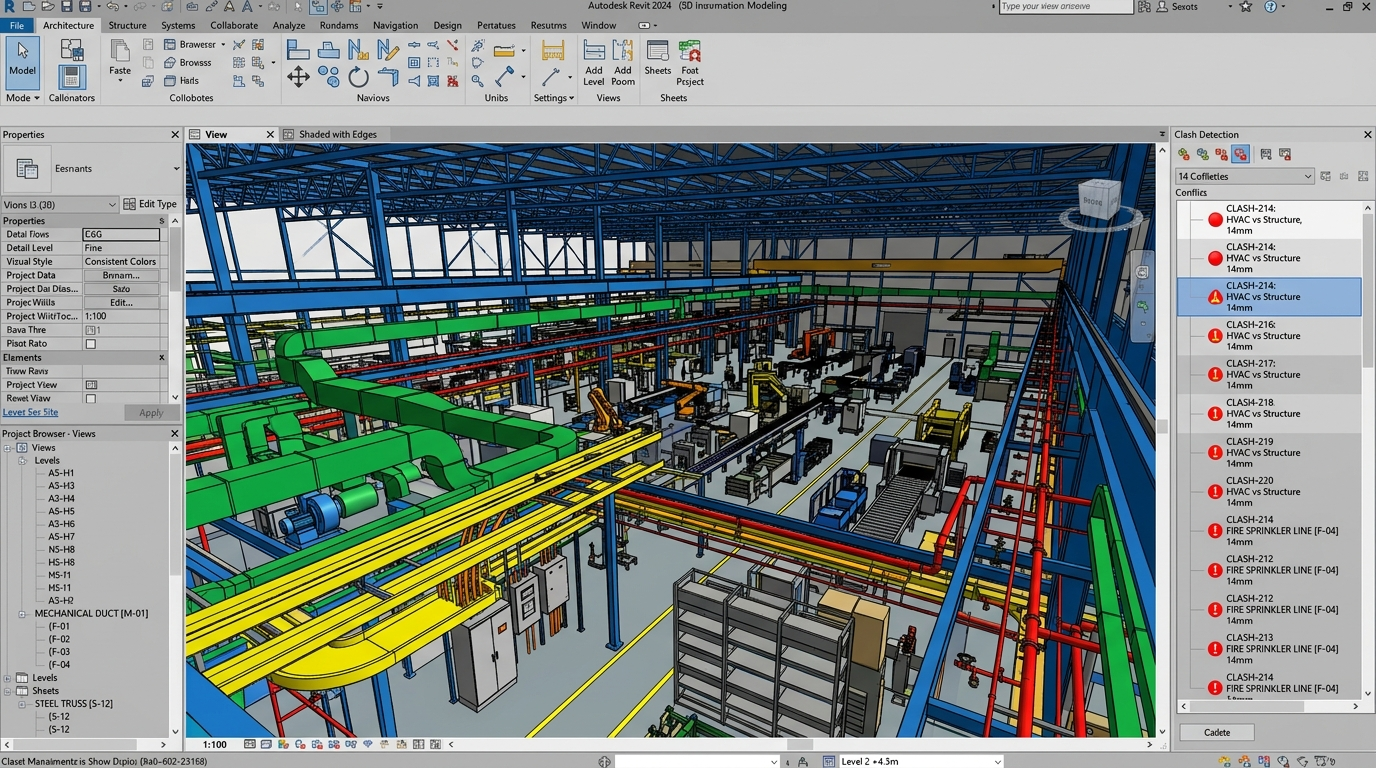
\includegraphics[width=186mm]{../../public/bim-model-3d.jpg}};
  \fill[TTCDeepNavy,opacity=.88] (0,0) rectangle (61,68);
  \fill[TTCDeepNavy,opacity=.24] (61,0) rectangle (86,68);
  \node[anchor=west,text width=48mm,align=left,text=white] at (8,44) {
    {\fontsize{7}{8}\selectfont\bfseries\color{TTCCyan} TTC DIGITAL THREAD}\\[1.4mm]
    {\fontsize{19}{21}\selectfont\bfseries DATA TO}\\[-.3mm]
    {\fontsize{19}{21}\selectfont\bfseries\color{TTCRed!85!white} DECISION}\\[1.8mm]
    {\fontsize{7}{8.5}\selectfont\color{white!82!gray}
    A reliable source of data for design, site and crew.}
  };
  \node[rounded corners=2pt,fill=white,align=center,minimum width=27mm,
        minimum height=15mm] at (111,15) {
    {\fontsize{9}{10}\selectfont\bfseries\color{TTCBlue} DESIGN}\\[-.2mm]
    {\fontsize{5.8}{7}\selectfont LOD 400 • 5D}
  };
  \node[rounded corners=2pt,fill=TTCCyan,align=center,text=white,
        minimum width=27mm,minimum height=15mm] at (143,15) {
    {\fontsize{9}{10}\selectfont\bfseries BUILD}\\[-.2mm]
    {\fontsize{5.8}{7}\selectfont Clash • 4D}
  };
  \node[rounded corners=2pt,fill=TTCGold,align=center,text=white,
        minimum width=27mm,minimum height=15mm] at (172,15) {
    {\fontsize{9}{10}\selectfont\bfseries OPERATE}\\[-.2mm]
    {\fontsize{5.8}{7}\selectfont Twin • O\&M}
  };
\end{tikzpicture}

\vspace{3mm}

% THREE DECISION ENGINES
\noindent
\begin{tikzpicture}[x=1mm,y=1mm]
  \path[use as bounding box] (0,0) rectangle (186,62);
  \foreach \x/\c in {0/TTCRed,63/TTCCyan,126/TTCGold}{
    \fill[white,rounded corners=2pt] (\x,0) rectangle +(60,62);
    \draw[TTCBorder,rounded corners=2pt,line width=.6pt] (\x,0) rectangle +(60,62);
    \fill[\c,rounded corners=2pt] (\x,58) rectangle +(60,4);
  }
  \node[anchor=north west,text width=50mm] at (5,53) {
    {\fontsize{7}{8}\selectfont\bfseries\color{TTCRed} 01 / COORDINATE}\\[1mm]
    {\fontsize{11}{12}\selectfont\bfseries\color{TTCBlue} BIM 5D}\\[1.2mm]
    {\fontsize{6.8}{8.2}\selectfont\color{TTCTextDark}
    \textbf{Input:} Architecture • Structure • MEP\newline
    \textbf{Decision:} Clash-check and sequence\newline
    \textbf{Output:} Shop Drawing, BOQ, 4D plan}\\[1mm]
    {\fontsize{6.2}{7.3}\selectfont\bfseries\color{TTCTextMuted} TEKLA • REVIT • NAVISWORKS}
  };
  \node[anchor=north west,text width=50mm] at (68,53) {
    {\fontsize{7}{8}\selectfont\bfseries\color{TTCCyan} 02 / OPTIMIZE}\\[1mm]
    {\fontsize{11}{12}\selectfont\bfseries\color{TTCBlue} AI STRUCTURE}\\[1.2mm]
    {\fontsize{6.8}{8.2}\selectfont\color{TTCTextDark}
    \textbf{Input:} Load • span • internal force\newline
    \textbf{Decision:} Repeat the sectional plan\newline
    \textbf{Output:} Section plan for the engineer to check}\\[1mm]
    {\fontsize{6.2}{7.3}\selectfont\bfseries\color{TTCTextMuted} AISC 360 • TCVN • AIDC R\&D}
  };
  \node[anchor=north west,text width=50mm] at (131,53) {
    {\fontsize{7}{8}\selectfont\bfseries\color{TTCGold} 03 / OPERATE}\\[1mm]
    {\fontsize{11}{12}\selectfont\bfseries\color{TTCBlue} DIGITAL TWIN}\\[1.2mm]
    {\fontsize{6.8}{8.2}\selectfont\color{TTCTextDark}
    \textbf{Input:} As-built • assets • IoT\newline
    \textbf{Decision:} Status-based maintenance\newline
    \textbf{Output:} Traceable operating records}\\[1mm]
    {\fontsize{6.2}{7.3}\selectfont\bfseries\color{TTCTextMuted} CDE • BMS • SCADA READY}
  };
\end{tikzpicture}

\vspace{3mm}

% DIGITAL THREAD FLOW
\noindent
\begin{tikzpicture}[x=1mm,y=1mm]
  \path[use as bounding box] (0,0) rectangle (186,42);
  \fill[TTCLightBlue,rounded corners=3pt] (0,0) rectangle (186,42);
  \draw[TTCBorder,rounded corners=3pt,line width=.6pt] (0,0) rectangle (186,42);
  \node[anchor=west,text=TTCBlue,font=\fontsize{8}{9.5}\selectfont\bfseries] at (7,34)
    {\faDatabase\quad DIGITAL THREAD — DATA NOT BROKEN};
  \foreach \x/\n/\t in {24/01/MODEL,70/02/APPROVE,116/03/BUILD,162/04/OPERATE}{
    \fill[white] (\x,17) circle (5);
    \draw[TTCBlue,line width=.8pt] (\x,17) circle (5);
    \node[text=TTCRed,font=\fontsize{6.4}{7}\selectfont\bfseries] at (\x,17) {\n};
    \node[anchor=north,align=center,text width=34mm] at (\x,9) {
      {\fontsize{6.7}{8}\selectfont\bfseries\color{TTCBlue} \t}
    };
  }
  \draw[-{Stealth[length=2.2mm]},TTCBlue!45!white,line width=.9pt] (30,17) -- (64,17);
  \draw[-{Stealth[length=2.2mm]},TTCBlue!45!white,line width=.9pt] (76,17) -- (110,17);
  \draw[-{Stealth[length=2.2mm]},TTCBlue!45!white,line width=.9pt] (122,17) -- (156,17);
\end{tikzpicture}

\vspace{3mm}

% KPI MEMORY STRIP
\noindent
\begin{tikzpicture}[x=1mm,y=1mm]
  \path[use as bounding box] (0,0) rectangle (186,29);
  \fill[TTCDeepNavy,rounded corners=3pt] (0,0) rectangle (186,29);
  \foreach \x in {46.5,93,139.5}{\draw[white!35!gray] (\x,6) -- (\x,23);}
  \node[align=center,text=white] at (23.25,15) {{\fontsize{9}{10}\selectfont\bfseries\color{TTCRed} LOD 400}\\[-.3mm]{\fontsize{6.2}{7.4}\selectfont Fabrication Detail}};
  \node[align=center,text=white] at (69.75,15) {{\fontsize{9}{10}\selectfont\bfseries\color{TTCCyan} REVIEWED}\\[-.3mm]{\fontsize{6.2}{7.4}\selectfont Engineering Options}};
  \node[align=center,text=white] at (116.25,15) {{\fontsize{9}{10}\selectfont\bfseries COORDINATED}\\[-.3mm]{\fontsize{6.2}{7.4}\selectfont Model Interfaces}};
  \node[align=center,text=white] at (162.75,15) {{\fontsize{9}{10}\selectfont\bfseries\color{TTCGold} TRACEABLE}\\[-.3mm]{\fontsize{6.2}{7.4}\selectfont Handover Data}};
\end{tikzpicture}
\end{minipage}
\newpage

% ============================================================
% PAGE 16: ESG BUSINESS CASE — GREEN FACTORY
% ============================================================
\pageheaderbar{GREEN BUILDINGS \& SOLAR-READY ROOFS}{Page 16}
\pagefooterbar{Page 16}

\begin{tikzpicture}[remember picture, overlay]
  \fill[TTCLightBlue]
    ([xshift=125mm,yshift=-30mm]current page.north west) --
    ([xshift=210mm,yshift=-30mm]current page.north west) --
    ([xshift=210mm,yshift=-112mm]current page.north west) -- cycle;
  \node[opacity=.03,text=TTCBlue,font=\fontsize{64}{66}\selectfont\bfseries,
        rotate=90] at ([xshift=-11mm,yshift=2mm]current page.east) {ESG};
  % Solar roof rhythm at the bottom
  \begin{scope}[shift={(current page.south west)},x=1mm,y=1mm,opacity=.43]
    \draw[TTCBlue!17!white,line width=.7pt] (14,13) -- (196,13);
    \foreach \x in {18,48,78,108,138,168}{
      \fill[TTCBlue!3!white] (\x,14) -- ++(24,0) -- ++(-5,17) -- ++(-24,0) -- cycle;
      \draw[TTCBlue!16!white] (\x,14) -- ++(24,0) -- ++(-5,17) -- ++(-24,0) -- cycle;
      \draw[TTCBlue!11!white] (\x+4,14) -- (\x-1,31);
      \draw[TTCBlue!11!white] (\x+12,14) -- (\x+7,31);
    }
    \draw[TTCCyan!22!white,line width=.8pt] (24,38) arc[start angle=210,end angle=330,radius=10mm];
    \draw[TTCRed!18!white,line width=.7pt] (24,38) -- (24,45);
  \end{scope}
\end{tikzpicture}

\begin{minipage}[t][246mm]{\textwidth}
\secbrand{Green Factories Designed as a Business Case}{Solar-Ready, Low-Energy Envelope, Water Circularity \& Green Certification}

{\fontsize{15}{17}\selectfont\bfseries\color{TTCBlue}
DECREASE IN OPEX • CARBON READINESS • INCREASE IN ASSET VALUE\par}
\vspace{1mm}
{\fontsize{7.5}{9}\selectfont\color{TTCTextMuted}
ESG is built from structural and enclosure — not costly replenishment once the plant is up and running.\par}
\vspace{3mm}

% HERO — GREEN FACTORY
\noindent
\begin{tikzpicture}[x=1mm,y=1mm]
  \path[use as bounding box] (0,0) rectangle (186,70);
  \clip[rounded corners=3pt] (0,0) rectangle (186,70);
  \node[anchor=center,inner sep=0pt] at (93,35)
    {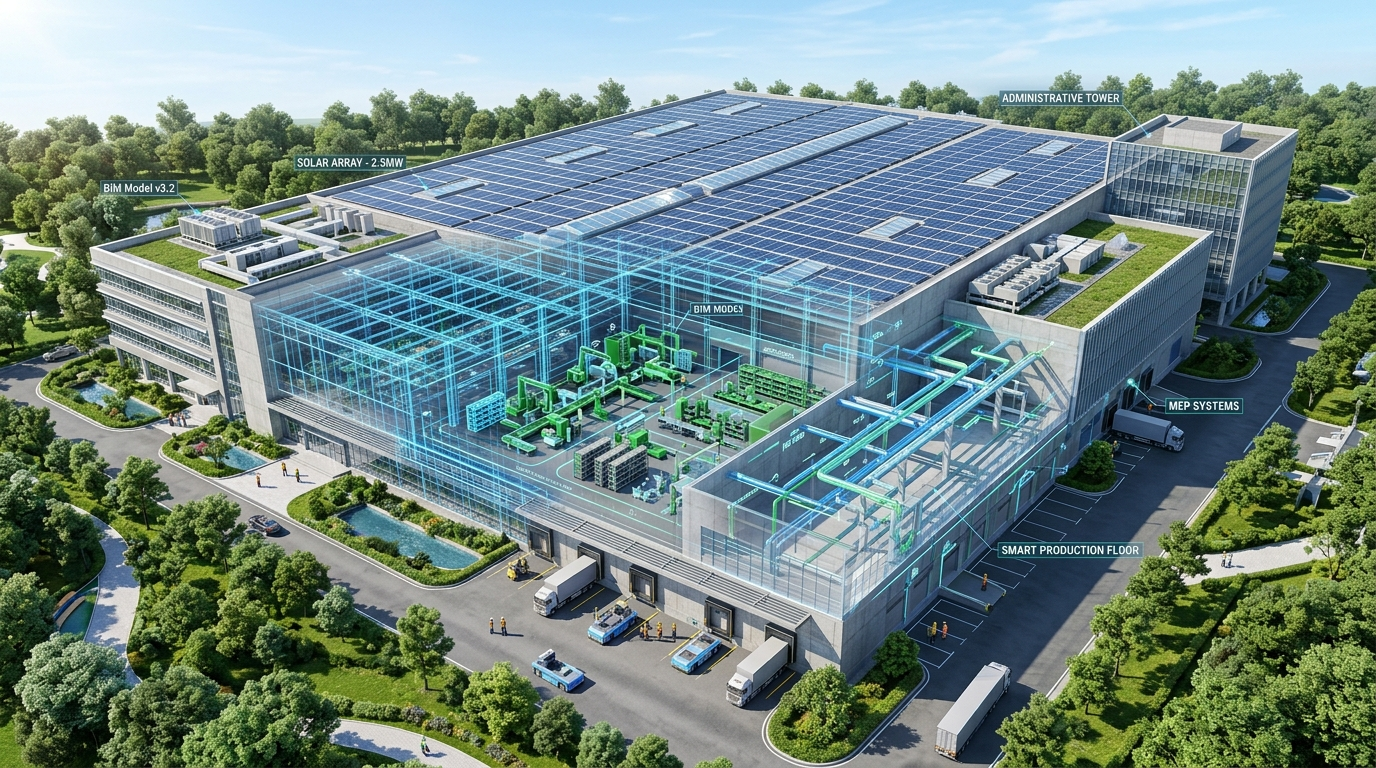
\includegraphics[width=186mm]{../../public/bim-esg-factory-3d.jpg}};
  \fill[TTCDeepNavy,opacity=.84] (0,0) rectangle (61,70);
  \fill[TTCDeepNavy,opacity=.22] (61,0) rectangle (87,70);
  \node[anchor=west,text width=48mm,align=left,text=white] at (8,46) {
    {\fontsize{7}{8}\selectfont\bfseries\color{TTCCyan} ESG-BY-DESIGN}\\[1.3mm]
    {\fontsize{17}{19}\selectfont\bfseries NET-ZERO}\\[-.2mm]
    {\fontsize{17}{19}\selectfont\bfseries\color{TTCRed!85!white} READY}\\[1.8mm]
    {\fontsize{7}{8.5}\selectfont\color{white!82!gray}
    Structure, energy, water and operation are prepared in the same model.}
  };
  \node[rounded corners=2pt,fill=white,align=center,minimum width=31mm,
        minimum height=15mm] at (121,15) {
    {\fontsize{10}{11}\selectfont\bfseries\color{TTCRed} SOLAR}\\[-.2mm]
    {\fontsize{5.8}{7}\selectfont\color{TTCBlue} SOLAR-READY}
  };
  \node[rounded corners=2pt,fill=TTCCyan,align=center,text=white,
        minimum width=31mm,minimum height=15mm] at (155,15) {
    {\fontsize{10}{11}\selectfont\bfseries PASSIVE}\\[-.2mm]
    {\fontsize{5.8}{7}\selectfont ENVELOPE DESIGN}
  };
\end{tikzpicture}

\vspace{3mm}

% FOUR ESG LEVERS
\noindent
\begin{tikzpicture}[x=1mm,y=1mm]
  \path[use as bounding box] (0,0) rectangle (186,51);
  \foreach \x/\c in {0/TTCRed,47.5/TTCCyan,95/TTCBlue,142.5/TTCGold}{
    \fill[white,rounded corners=2pt] (\x,0) rectangle +(43.5,51);
    \draw[TTCBorder,rounded corners=2pt,line width=.6pt] (\x,0) rectangle +(43.5,51);
    \fill[\c,rounded corners=2pt] (\x,47) rectangle +(43.5,4);
  }
  \node[anchor=north west,text width=35mm] at (4,43) {
    {\fontsize{7}{8}\selectfont\bfseries\color{TTCRed} 01 / ENERGY}\\[1mm]
    {\fontsize{8.5}{10}\selectfont\bfseries\color{TTCBlue} SOLAR-READY}\\[1mm]
    {\fontsize{6.5}{7.8}\selectfont\color{TTCTextDark}
    Provision for roof loading, purlins and installation interface according to approved battery system data.}
  };
  \node[anchor=north west,text width=35mm] at (51.5,43) {
    {\fontsize{7}{8}\selectfont\bfseries\color{TTCCyan} 02 / ENVELOPE}\\[1mm]
    {\fontsize{8.5}{10}\selectfont\bfseries\color{TTCBlue} COOL ROOF}\\[1mm]
    {\fontsize{6.5}{7.8}\selectfont\color{TTCTextDark}
    PIR/Rockwool panel and HVAC load-reducing heat-reflective roof.}
  };
  \node[anchor=north west,text width=35mm] at (99,43) {
    {\fontsize{7}{8}\selectfont\bfseries\color{TTCBlue} 03 / WATER}\\[1mm]
    {\fontsize{8.5}{10}\selectfont\bfseries\color{TTCBlue} CIRCULARITY}\\[1mm]
    {\fontsize{6.5}{7.8}\selectfont\color{TTCTextDark}
    Column A wastewater, rainwater collection and reuse for the landscape.}
  };
  \node[anchor=north west,text width=35mm] at (146.5,43) {
    {\fontsize{7}{8}\selectfont\bfseries\color{TTCGold} 04 / STANDARD}\\[1mm]
    {\fontsize{8.5}{10}\selectfont\bfseries\color{TTCBlue} LEED / LOTUS}\\[1mm]
    {\fontsize{6.5}{7.8}\selectfont\color{TTCTextDark}
    Energy simulation, Low-VOC materials and certification records.}
  };
\end{tikzpicture}

\vspace{3mm}

% ESG BUSINESS CASE
\noindent
\begin{tikzpicture}[x=1mm,y=1mm]
  \path[use as bounding box] (0,0) rectangle (186,47);
  \fill[TTCLightBlue,rounded corners=3pt] (0,0) rectangle (186,47);
  \draw[TTCBorder,rounded corners=3pt,line width=.6pt] (0,0) rectangle (186,47);
  \node[anchor=west,text=TTCBlue,font=\fontsize{8}{9.5}\selectfont\bfseries] at (7,39)
    {\faGlobeAmericas\quad VALUE FOR INTERNATIONAL INVESTORS};
  \foreach \x in {62,124}{\draw[TTCBorder] (\x,6) -- (\x,31);}
  \node[align=left,text width=50mm,anchor=north west] at (6,30) {
    {\fontsize{8}{9.5}\selectfont\bfseries\color{TTCRed} GREEN FINANCE}\\[.7mm]
    {\fontsize{6.5}{7.8}\selectfont\color{TTCTextDark}
    Increase access to green capital and international supply chain criteria.}
  };
  \node[align=left,text width=50mm,anchor=north west] at (68,30) {
    {\fontsize{8}{9.5}\selectfont\bfseries\color{TTCCyan} CARBON READY}\\[.7mm]
    {\fontsize{6.5}{7.8}\selectfont\color{TTCTextDark}
    Prepare energy data, materials and emission reduction pathways as required by the project.}
  };
  \node[align=left,text width=50mm,anchor=north west] at (130,30) {
    {\fontsize{8}{9.5}\selectfont\bfseries\color{TTCGold} LOWER OPEX}\\[.7mm]
    {\fontsize{6.5}{7.8}\selectfont\color{TTCTextDark}
    Reduce HVAC power, optimize operating water and increase the value of asset exploitation.}
  };
\end{tikzpicture}

\vspace{3mm}

% KPI MEMORY STRIP
\noindent
\begin{tikzpicture}[x=1mm,y=1mm]
  \path[use as bounding box] (0,0) rectangle (186,29);
  \fill[TTCDeepNavy,rounded corners=3pt] (0,0) rectangle (186,29);
  \foreach \x in {46.5,93,139.5}{\draw[white!35!gray] (\x,6) -- (\x,23);}
  \node[align=center,text=white] at (23.25,15) {{\fontsize{9}{10}\selectfont\bfseries\color{TTCRed} SOLAR-READY}\\[-.3mm]{\fontsize{6.2}{7.4}\selectfont Approved System Data}};
  \node[align=center,text=white] at (69.75,15) {{\fontsize{9}{10}\selectfont\bfseries\color{TTCCyan} LOW-ENERGY}\\[-.3mm]{\fontsize{6.2}{7.4}\selectfont Envelope Strategy}};
  \node[align=center,text=white] at (116.25,15) {{\fontsize{9}{10}\selectfont\bfseries WATER}\\[-.3mm]{\fontsize{6.2}{7.4}\selectfont Project Requirements}};
  \node[align=center,text=white] at (162.75,15) {{\fontsize{9}{10}\selectfont\bfseries\color{TTCGold} GREEN DOSSIER}\\[-.3mm]{\fontsize{6.2}{7.4}\selectfont Certification Support}};
\end{tikzpicture}
\end{minipage}
\newpage

% ============================================================
% PAGE 17: DIGITAL SITE CONTROL CENTER
% ============================================================
\pageheaderbar{DIGITAL SITE CONTROL CENTRE}{Page 17}
\pagefooterbar{Page 17}

\begin{tikzpicture}[remember picture, overlay]
  \fill[TTCLightBlue]
    ([xshift=131mm,yshift=-30mm]current page.north west) --
    ([xshift=210mm,yshift=-30mm]current page.north west) --
    ([xshift=210mm,yshift=-115mm]current page.north west) -- cycle;
  % Data pulse background — deliberately different from the previous pages
  \begin{scope}[shift={(current page.south west)},x=1mm,y=1mm,opacity=.45]
    \draw[TTCBlue!18!white,line width=.8pt] (13,17) -- (197,17);
    \draw[TTCBlue!15!white] (20,17) -- (38,35) -- (62,25) -- (86,45) --
      (112,29) -- (139,42) -- (164,26) -- (191,38);
    \foreach \x/\y in {20/17,38/35,62/25,86/45,112/29,139/42,164/26,191/38}{
      \fill[TTCCyan!20!white] (\x,\y) circle (1.7);
      \draw[TTCBlue!20!white] (\x,\y) circle (3.1);
    }
  \end{scope}
\end{tikzpicture}

\begin{minipage}[t][246mm]{\textwidth}
\secbrand{Digital Site Control Centre}{Centralized data • Instant alerts • Retrievable records}

{\fontsize{15}{17}\selectfont\bfseries\color{TTCBlue}
ONE SITE • THREE DATA SOURCES • OPERATING ONE CONTRACT\par}
\vspace{1mm}
{\fontsize{7.5}{9}\selectfont\color{TTCTextMuted}
Gather human data, safety and construction documents for the Site Manager to handle the right work at the right time.\par}
\vspace{3mm}

% CONTROL CENTER DASHBOARD
\noindent
\begin{tikzpicture}[x=1mm,y=1mm]
  \path[use as bounding box] (0,0) rectangle (186,101);
  \fill[TTCDeepNavy,rounded corners=3pt] (0,0) rectangle (186,101);
  \draw[TTCCyan!65!white,rounded corners=3pt,line width=.8pt] (0,0) rectangle (186,101);

  \node[anchor=west,text=white,font=\fontsize{8}{9.5}\selectfont\bfseries] at (8,93)
    {\faDesktop\quad TRUNG DEDICATION};
  \node[anchor=east,text=TTCCyan,font=\fontsize{6.3}{7.5}\selectfont\bfseries] at (121,93)
    {REAL DATA • ACTIONS WITH TRACES};

  % Status row
  \foreach \x/\c in {8/TTCRed,47/TTCCyan,86/TTCGold}{
    \fill[white!7!TTCDeepNavy,rounded corners=2pt] (\x,63) rectangle +(34,21);
    \draw[\c!70!white,rounded corners=2pt,line width=.55pt] (\x,63) rectangle +(34,21);
  }
  \node[anchor=west,text=TTCRed,font=\fontsize{6.2}{7.3}\selectfont\bfseries] at (11,78) {ACCESS CONTROL};
  \node[anchor=west,text=white,font=\fontsize{9.2}{10.5}\selectfont\bfseries] at (11,70) {RIGHT PERSON};
  \node[anchor=west,text=TTCCyan,font=\fontsize{6.2}{7.3}\selectfont\bfseries] at (50,78) {GLOBAL SAFETY MONITORING};
  \node[anchor=west,text=white,font=\fontsize{9.2}{10.5}\selectfont\bfseries] at (50,70) {CORRECT};
  \node[anchor=west,text=TTCGold,font=\fontsize{6.2}{7.3}\selectfont\bfseries] at (89,78) {COMPANY ON SITE};
  \node[anchor=west,text=white,font=\fontsize{9.2}{10.5}\selectfont\bfseries] at (89,70) {CORRECT VERSION};

  % Three real data streams
  \fill[white,rounded corners=2pt] (8,29) rectangle (40,55);
  \fill[white,rounded corners=2pt] (47,29) rectangle (79,55);
  \fill[white,rounded corners=2pt] (86,29) rectangle (118,55);
  \node[align=center,text width=27mm] at (24,42) {
    {\fontsize{7.5}{9}\selectfont\bfseries\color{TTCRed} PERSONNEL}\\[-.2mm]
    {\fontsize{6.2}{7.4}\selectfont\color{TTCTextMuted}FaceID • training\\gateway certificate}
  };
  \node[align=center,text width=27mm] at (63,42) {
    {\fontsize{7.5}{9}\selectfont\bfseries\color{TTCCyan} SAFETY FULL}\\[-.2mm]
    {\fontsize{6.2}{7.4}\selectfont\color{TTCTextMuted}Camera AI • PPE\\danger zone}
  };
  \node[align=center,text width=27mm] at (102,42) {
    {\fontsize{7.5}{9}\selectfont\bfseries\color{TTCGold} COMPANY}\\[-.2mm]
    {\fontsize{6.2}{7.4}\selectfont\color{TTCTextMuted}CDE • ITP • RFI\\digital logbook}
  };
  \draw[-{Stealth[length=2mm]},TTCCyan,line width=.8pt] (40.5,42) -- (46,42);
  \draw[-{Stealth[length=2mm]},TTCCyan,line width=.8pt] (79.5,42) -- (85,42);

  % Decision layer
  \fill[TTCCyan!12!TTCDeepNavy,rounded corners=2pt] (8,7) rectangle (118,21);
  \node[anchor=west,text=TTCCyan,font=\fontsize{6}{7}\selectfont\bfseries] at (12,14)
    {EXECUTIVE CLASS};
  \node[anchor=west,text=white,font=\fontsize{7}{8.5}\selectfont\bfseries] at (40,14)
    {→ Roster → Approval → Warning Save Evidence};

  % Ảnh hiện trường có vùng chú thích riêng, không đặt chữ lên ảnh
  \begin{scope}
    \clip[rounded corners=2pt] (126,16) rectangle (179,86);
    \node[anchor=center,inner sep=0pt] at (152.5,51)
      {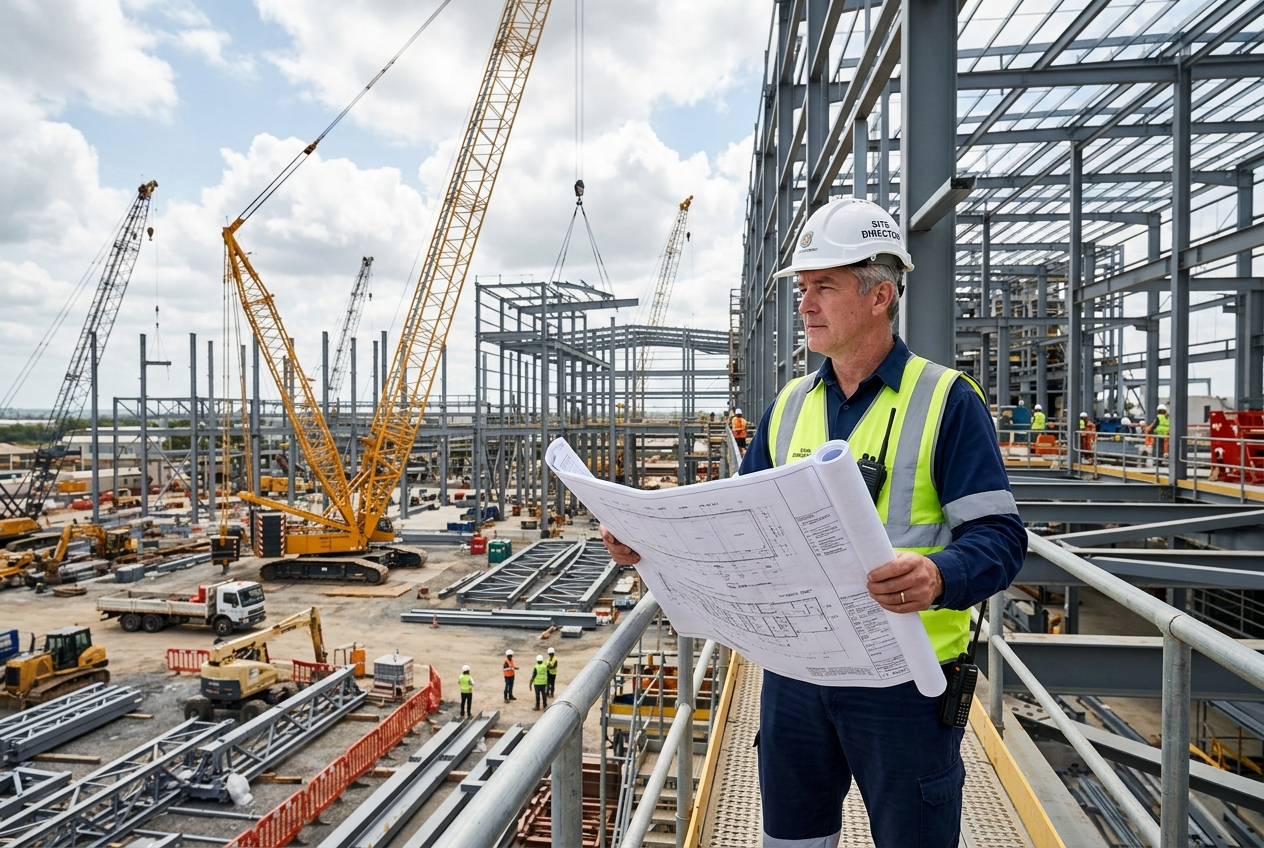
\includegraphics[height=70mm]{../../public/c_level_site_inspection.jpg}};
  \end{scope}
  \draw[white!45!gray,rounded corners=2pt,line width=.6pt] (126,16) rectangle (179,86);
  \fill[TTCBlue] (126,7) rectangle (179,15);
  \node[text=white,font=\fontsize{6.4}{7.5}\selectfont\bfseries] at (152.5,11)
    {IMAGE OF THE SCENE};
\end{tikzpicture}

\vspace{3mm}

% OWNER VIEW — THREE OUTCOMES
\noindent
\begin{tikzpicture}[x=1mm,y=1mm]
  \path[use as bounding box] (0,0) rectangle (186,49);
  \fill[white,rounded corners=3pt] (0,0) rectangle (186,49);
  \draw[TTCBorder,rounded corners=3pt,line width=.6pt] (0,0) rectangle (186,49);
  \node[anchor=west,text=TTCBlue,font=\fontsize{8}{9.5}\selectfont\bfseries] at (7,41)
    {\faMobile*\quad INFORMATION SUFFICIENT FOR DECISION MAKING};
  \foreach \x in {62,124}{\draw[TTCBorder] (\x,7) -- (\x,33);}
  \node[anchor=north west,text width=50mm] at (6,31) {
    {\fontsize{8}{9.5}\selectfont\bfseries\color{TTCRed} TROOPS READY}\\[.7mm]
    {\fontsize{6.6}{8}\selectfont\color{TTCTextDark}
    Know who is at the construction site and the entry conditions of each person.}
  };
  \node[anchor=north west,text width=50mm] at (68,31) {
    {\fontsize{8}{9.5}\selectfont\bfseries\color{TTCCyan} SAFETY FULL VIEW}\\[.7mm]
    {\fontsize{6.6}{8}\selectfont\color{TTCTextDark}
    PPE violation and hazardous zone intrusion alerts for immediate processing.}
  };
  \node[anchor=north west,text width=50mm] at (130,31) {
    {\fontsize{8}{9.5}\selectfont\bfseries\color{TTCGold} FULL COMPANY}\\[.7mm]
    {\fontsize{6.6}{8}\selectfont\color{TTCTextDark}
    Diary, RFI and ITP records with time, approver and evidence.}
  };
\end{tikzpicture}

\vspace{3mm}

% ACTION LOOP — NO KPI GRID
\noindent
\begin{tikzpicture}[x=1mm,y=1mm]
  \path[use as bounding box] (0,0) rectangle (186,43);
  \fill[TTCLightBlue,rounded corners=3pt] (0,0) rectangle (186,43);
  \draw[TTCBorder,rounded corners=3pt,line width=.6pt] (0,0) rectangle (186,43);
  \node[anchor=west,text=TTCBlue,font=\fontsize{8}{9.5}\selectfont\bfseries] at (7,35)
    {\faCheckCircle\quad ACTION LOOP OF THE DAY};
  \foreach \x/\n/\t in {23/01/RECORDING, 69/02/WARNING ,115/03/HANDLING ,161/04/TRACKING}{
    \fill[white] (\x,17) circle (5);
    \draw[TTCBlue,line width=.8pt] (\x,17) circle (5);
    \node[text=TTCRed,font=\fontsize{6.3}{7}\selectfont\bfseries] at (\x,17) {\n};
    \node[anchor=north,align=center,text width=34mm] at (\x,9)
      {{\fontsize{6.7}{8}\selectfont\bfseries\color{TTCBlue} \t}};
  }
  \draw[-{Stealth[length=2mm]},TTCBlue!45!white,line width=.9pt] (29,17) -- (63,17);
  \draw[-{Stealth[length=2mm]},TTCBlue!45!white,line width=.9pt] (75,17) -- (109,17);
  \draw[-{Stealth[length=2mm]},TTCBlue!45!white,line width=.9pt] (121,17) -- (155,17);
\end{tikzpicture}
\end{minipage}
\newpage

% ============================================================
% PAGE 18: QUALITY PASSPORT & RELEASE GATES
% ============================================================
\pageheaderbar{QA/QC MANAGEMENT SYSTEM}{Page 18}
\pagefooterbar{Page 18}

\begin{tikzpicture}[remember picture, overlay]
  \fill[TTCLightBlue]
    ([xshift=121mm,yshift=-31mm]current page.north west) --
    ([xshift=210mm,yshift=-31mm]current page.north west) --
    ([xshift=210mm,yshift=-118mm]current page.north west) -- cycle;
  % document trace lines at the bottom
  \begin{scope}[shift={(current page.south west)},x=1mm,y=1mm,opacity=.43]
    \draw[TTCBlue!17!white,line width=.7pt] (14,15) -- (196,15);
    \foreach \x in {18,56,94,132,170}{
      \draw[TTCBlue!15!white,rounded corners=1pt] (\x,15) rectangle +(25,28);
      \draw[TTCRed!14!white] (\x+5,35) -- (\x+20,35);
      \draw[TTCBlue!11!white] (\x+5,29) -- (\x+20,29);
      \draw[TTCBlue!11!white] (\x+5,23) -- (\x+16,23);
    }
  \end{scope}
\end{tikzpicture}

\begin{minipage}[t][246mm]{\textwidth}
\secbrand{A Quality Passport for Every Work Package}{Four-level ITP control • Enough evidence to move forward}

{\fontsize{15}{17}\selectfont\bfseries\color{TTCBlue}
ONLY MOVE FORWARD WHEN THERE IS SUFFICIENT EVIDENCE\par}
\vspace{1mm}
{\fontsize{7.5}{9}\selectfont\color{TTCTextMuted}
Each material, weld and item is inspected, signed and traced prior to release for the next step.\par}
\vspace{3mm}

% QUALITY GATES + PASSPORT
\noindent
\begin{tikzpicture}[x=1mm,y=1mm]
  \path[use as bounding box] (0,0) rectangle (186,122);

  % Left release ladder
  \fill[TTCDeepNavy,rounded corners=3pt] (0,0) rectangle (57,122);
  \node[anchor=west,text=TTCCyan,font=\fontsize{7}{8}\selectfont\bfseries] at (6,113)
    {4 LEVELS OF CONTROL};
  \node[anchor=west,text=white,font=\fontsize{11}{12}\selectfont\bfseries] at (6,106.5)
    {ITP PORT};

  \foreach \y/\n/\c in {78/01/TTCRed,52/02/TTCBlue,26/03/TTCCyan,0/04/TTCGold}{
    \fill[white,rounded corners=2pt] (6,\y+6) rectangle (51,\y+25);
    \draw[\c,rounded corners=2pt,line width=.7pt] (6,\y+6) rectangle (51,\y+25);
    \fill[\c] (6,\y+6) rectangle (13,\y+25);
    \node[text=white,font=\fontsize{6.5}{7}\selectfont\bfseries] at (9.5,\y+15.5) {\n};
  }
  \node[anchor=west,text width=33mm] at (16,93.5) {
    {\fontsize{7.2}{8.5}\selectfont\bfseries\color{TTCRed} SELF-INSPECTION TEAM}\\[-.2mm]
    {\fontsize{6.2}{7.4}\selectfont\color{TTCTextMuted}Internal Checklist}
  };
  \node[anchor=west,text width=33mm] at (16,67.5) {
    {\fontsize{7.2}{8.5}\selectfont\bfseries\color{TTCBlue} SITE ENGINEER}\\[-.2mm]
    {\fontsize{6.2}{7.4}\selectfont\color{TTCTextMuted}Shop Drawings • ITP}
  };
  \node[anchor=west,text width=33mm] at (16,41.5) {
    {\fontsize{7.2}{8.5}\selectfont\bfseries\color{TTCCyan} INDEPENDENT QA/QC}\\[-.2mm]
    {\fontsize{6.2}{7.4}\selectfont\color{TTCTextMuted}NDT minutes • test results}
  };
  \node[anchor=west,text width=33mm] at (16,15.5) {
    {\fontsize{7.2}{8.5}\selectfont\bfseries\color{TTCGold} SUPERVISION CONSULTANT / INVESTOR}\\[-.2mm]
    {\fontsize{6.2}{7.4}\selectfont\color{TTCTextMuted}Final approval}
  };
  \draw[-{Stealth[length=2mm]},white!55!gray,line width=.8pt] (28.5,83) -- (28.5,78);
  \draw[-{Stealth[length=2mm]},white!55!gray,line width=.8pt] (28.5,57) -- (28.5,52);
  \draw[-{Stealth[length=2mm]},white!55!gray,line width=.8pt] (28.5,31) -- (28.5,26);

  % Right quality passport
  \fill[white,rounded corners=3pt] (62,0) rectangle (186,122);
  \draw[TTCBorder,rounded corners=3pt,line width=.7pt] (62,0) rectangle (186,122);
  \fill[TTCLightBlue,rounded corners=3pt] (62,101) rectangle (186,122);
  \node[anchor=west,text=TTCBlue,font=\fontsize{10}{11.5}\selectfont\bfseries] at (68,113)
    {\faClipboardCheck\quad COMPANY ITEM QUALITY};
  \node[anchor=east,text=TTCTextMuted,font=\fontsize{6}{7}\selectfont\bfseries] at (180,113)
    {JOB PACKAGE CODE/COMPANY RETRIEVAL};

  \foreach \y/\n/\c in {78/01/TTCRed,55/02/TTCBlue,32/03/TTCCyan,9/04/TTCGold}{
    \fill[\c!6!white,rounded corners=1.5pt] (68,\y) rectangle (180,\y+18);
    \node[anchor=west,text=\c,font=\fontsize{7}{8}\selectfont\bfseries] at (72,\y+12) {\n};
    \fill[\c] (165,\y+5) circle (2.3);
    \node[text=white,font=\fontsize{5}{5.5}\selectfont\bfseries] at (165,\y+5) {\faCheck};
    \node[anchor=west,text=TTCTextMuted,font=\fontsize{6.1}{7.2}\selectfont\bfseries] at (170,\y+5) {PASS};
  }
  \node[anchor=west,text=TTCBlue,font=\fontsize{7.4}{8.7}\selectfont\bfseries] at (81,90) {MATERIAL ORIGIN};
  \node[anchor=west,text=TTCTextDark,font=\fontsize{6.3}{7.5}\selectfont] at (81,84) {CO/CQ • lot number • factory release certificate • input inspection};
  \node[anchor=west,text=TTCBlue,font=\fontsize{7.4}{8.7}\selectfont\bfseries] at (81,67) {WELDING CONTROL};
  \node[anchor=west,text=TTCTextDark,font=\fontsize{6.3}{7.5}\selectfont] at (81,61) {WPS/PQR • welder code • AWS D1.1 • weld diagram};
  \node[anchor=west,text=TTCBlue,font=\fontsize{7.4}{8.7}\selectfont\bfseries] at (81,44) {PROOF OF INSPECTION};
  \node[anchor=west,text=TTCTextDark,font=\fontsize{6.3}{7.5}\selectfont] at (81,38) {VT • UT • MT/PT • independent inspection record};
  \node[anchor=west,text=TTCBlue,font=\fontsize{7.4}{8.7}\selectfont\bfseries] at (81,21) {AS-BUILT COMPANY};
  \node[anchor=west,text=TTCTextDark,font=\fontsize{6.3}{7.5}\selectfont] at (81,15) {Signed ITP • Closed NCR • As-built drawing • save CDE};
\end{tikzpicture}

\vspace{3mm}

% NDT TOOLBOX
\noindent
\begin{tikzpicture}[x=1mm,y=1mm]
  \path[use as bounding box] (0,0) rectangle (186,46);
  \fill[TTCLightBlue,rounded corners=3pt] (0,0) rectangle (186,46);
  \draw[TTCBorder,rounded corners=3pt,line width=.6pt] (0,0) rectangle (186,46);
  \node[anchor=west,text=TTCBlue,font=\fontsize{8}{9.5}\selectfont\bfseries] at (7,38)
    {\faCheckDouble\quad NDT TEST METHOD};
  \foreach \x in {46.5,93,139.5}{\draw[TTCBorder] (\x,6) -- (\x,31);}
  \node[align=center,text width=38mm] at (23.25,18) {
    {\fontsize{9}{10}\selectfont\bfseries\color{TTCRed} VT}\\[-.2mm]
    {\fontsize{6.1}{7.3}\selectfont Appearance • size • surface}
  };
  \node[align=center,text width=38mm] at (69.75,18) {
    {\fontsize{9}{10}\selectfont\bfseries\color{TTCCyan} UT}\\[-.2mm]
    {\fontsize{6.3}{7.5}\selectfont Ultrasonic inspection of welds}
  };
  \node[align=center,text width=38mm] at (116.25,18) {
    {\fontsize{9}{10}\selectfont\bfseries\color{TTCBlue} MT / PT}\\[-.2mm]
    {\fontsize{6.3}{7.5}\selectfont Check surface cracks and corner joints}
  };
  \node[align=center,text width=38mm] at (162.75,18) {
    {\fontsize{9}{10}\selectfont\bfseries\color{TTCGold} LAS-XD}\\[-.2mm]
    {\fontsize{6.3}{7.5}\selectfont Laboratory testing}
  };
\end{tikzpicture}

\vspace{3mm}

% RELEASE OUTCOME
\noindent
\begin{tikzpicture}[x=1mm,y=1mm]
  \path[use as bounding box] (0,0) rectangle (186,30);
  \fill[TTCDeepNavy,rounded corners=3pt] (0,0) rectangle (186,30);
  \node[anchor=west,text=TTCCyan,font=\fontsize{7}{8}\selectfont\bfseries] at (8,20)
    {ISSUANCE GUIDELINES};
  \node[anchor=west,text=white,font=\fontsize{10}{11.5}\selectfont\bfseries] at (8,11)
    {VERIFIED → SUFFICIENT APPROVED PROOF → OF → RETRIEVAL};
  \node[anchor=east,text=TTCGold,font=\fontsize{12}{13}\selectfont\bfseries] at (178,15)
    {AWS D1.1 • ISO 9001};
\end{tikzpicture}
\end{minipage}
\newpage

% ============================================================
% PAGE 19: HSE DECISION SYSTEM & STOP WORK AUTHORITY
% ============================================================
\pageheaderbar{HSE \& STOP WORK AUTHORITY}{Page 19}
\pagefooterbar{Page 19}

\begin{tikzpicture}[remember picture, overlay]
  \fill[TTCRed!4!white]
    ([xshift=0mm,yshift=-210mm]current page.north west) --
    ([xshift=67mm,yshift=-248mm]current page.north west) --
    ([xshift=0mm,yshift=-278mm]current page.north west) -- cycle;
  \fill[TTCLightBlue]
    ([xshift=148mm,yshift=-31mm]current page.north west) --
    ([xshift=210mm,yshift=-31mm]current page.north west) --
    ([xshift=210mm,yshift=-108mm]current page.north west) -- cycle;
  \node[opacity=.035,text=TTCRed,font=\fontsize{66}{68}\selectfont\bfseries,
        rotate=90] at ([xshift=-11mm,yshift=-2mm]current page.east) {STOP};
\end{tikzpicture}

\begin{minipage}[t][246mm]{\textwidth}
\secbrand{Safety Is a Decision System — Not Just PPE}{Risk Elimination, Daily Control Cycle \& Stop Work Authority}

{\fontsize{15}{17}\selectfont\bfseries\color{TTCBlue}
SEES THE RISK • PRE-CONTROLS THE • STOPS WHEN SAFETY IS NOT SAFE\par}
\vspace{1mm}
{\fontsize{7.5}{9}\selectfont\color{TTCTextMuted}
Progress is never a reason to accept an uncontrolled working condition.\par}
\vspace{3mm}

% MANIFESTO + RISK HIERARCHY + DAILY LOOP
\noindent
\begin{tikzpicture}[x=1mm,y=1mm]
  \path[use as bounding box] (0,0) rectangle (186,149);

  % Left manifesto rail
  \fill[TTCDeepNavy,rounded corners=3pt] (0,0) rectangle (58,149);
  \begin{scope}
    \clip[rounded corners=3pt] (0,87) rectangle (58,149);
    \node[anchor=center,inner sep=0pt] at (29,118)
      {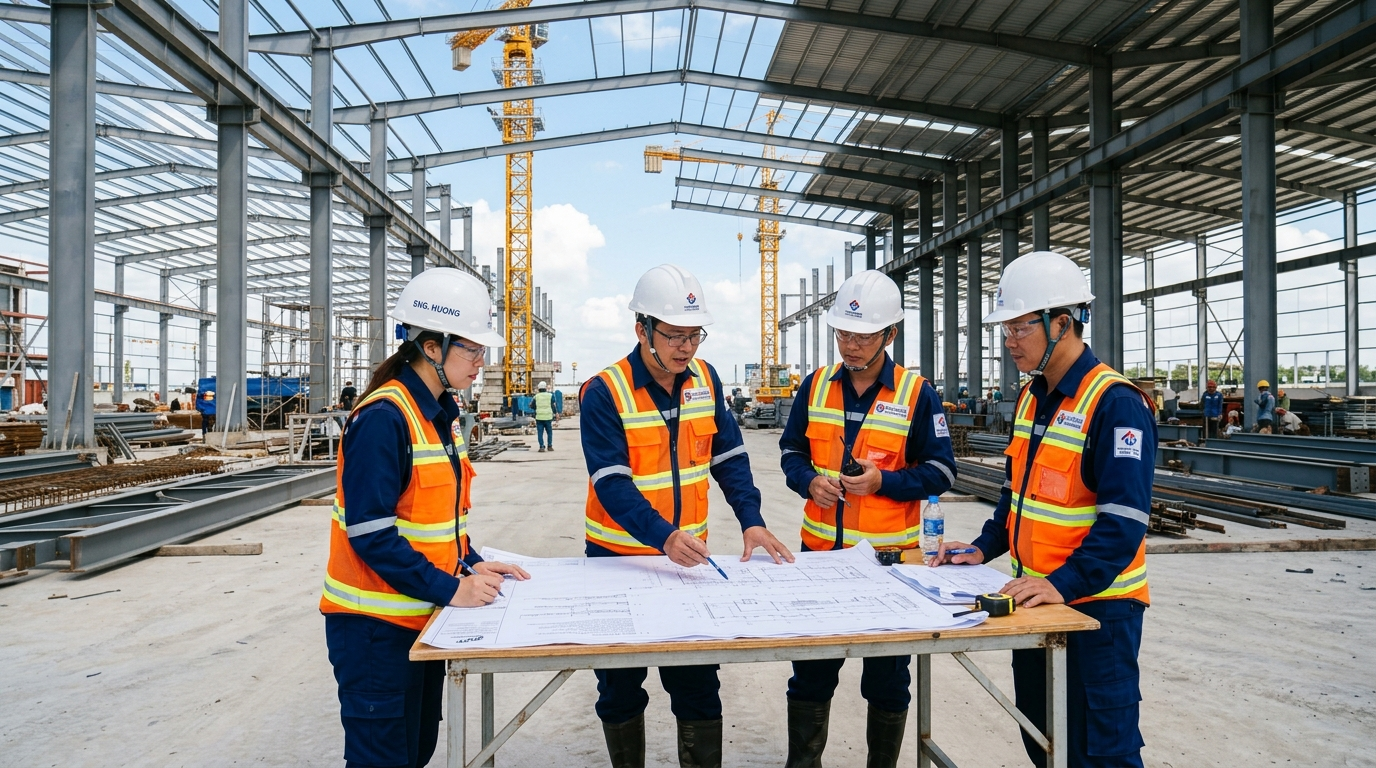
\includegraphics[height=62mm]{../../public/engineer-team-site.jpg}};
    \fill[TTCDeepNavy,opacity=.28] (0,87) rectangle (58,149);
  \end{scope}
  \node[anchor=west,text=TTCCyan,font=\fontsize{7}{8}\selectfont\bfseries] at (7,78)
    {STOP WORK AUTHORITY};
  \node[anchor=west,text=white,font=\fontsize{22}{23}\selectfont\bfseries] at (7,63)
    {STOP};
  \node[anchor=west,text=TTCRed!85!white,font=\fontsize{22}{23}\selectfont\bfseries] at (7,48)
    {WORK};
  \node[anchor=north west,text width=44mm,align=left] at (7,37) {
    {\fontsize{6.8}{8.3}\selectfont\color{white!85!gray}
    Anyone has the right to stop work when the safety condition is incomplete.}\\[2mm]
    {\fontsize{7}{8.5}\selectfont\bfseries\color{TTCGold}
    PEOPLE BEFORE PRODUCTION}
  };

  % Right — hierarchy of controls
  \fill[white,rounded corners=3pt] (63,86) rectangle (186,149);
  \draw[TTCBorder,rounded corners=3pt,line width=.6pt] (63,86) rectangle (186,149);
  \node[anchor=west,text=TTCBlue,font=\fontsize{8}{9.5}\selectfont\bfseries] at (69,141)
    {\faShield*\quad RISK CONTROL PRIORITY ORDER};

  \fill[TTCRed] (69,124) rectangle (180,136);
  \fill[TTCBlue] (74,111) rectangle (175,123);
  \fill[TTCCyan] (79,98) rectangle (170,110);
  \fill[TTCGold] (84,85) rectangle (165,97);
  \node[anchor=west,text=white,font=\fontsize{7}{8}\selectfont\bfseries] at (73,130) {01 • ELIMINATE — Eliminate the risk immediately from the measure};
  \node[anchor=west,text=white,font=\fontsize{7}{8}\selectfont\bfseries] at (78,117) {02 • ENGINEER — Barrier, working platform, fall protection};
  \node[anchor=west,text=white,font=\fontsize{7}{8}\selectfont\bfseries] at (83,104) {03 • PERMITS — JSA, licenses and supervisors};
  \node[anchor=west,text=white,font=\fontsize{7}{8}\selectfont\bfseries] at (88,91) {04 • PPE — Final protective layer};

  % Right — daily safety cycle
  \fill[TTCLightBlue,rounded corners=3pt] (63,29) rectangle (186,81);
  \draw[TTCBorder,rounded corners=3pt,line width=.6pt] (63,29) rectangle (186,81);
  \node[anchor=west,text=TTCBlue,font=\fontsize{8}{9.5}\selectfont\bfseries] at (69,73)
    {\faClock\quad DAILY SAFETY CONTROL CYCLE};
  \draw[TTCBlue!35!white,line width=1pt] (76,50) -- (175,50);
  \foreach \x/\n/\t in {77/01/PLAN,102/02/TALK,127/03/VERIFY,152/04/WORK,175/05/CLOSE}{
    \fill[white] (\x,50) circle (4.5);
    \draw[TTCBlue,line width=.75pt] (\x,50) circle (4.5);
    \node[text=TTCRed,font=\fontsize{5.8}{6.5}\selectfont\bfseries] at (\x,50) {\n};
    \node[anchor=north,align=center,text width=22mm] at (\x,42)
      {{\fontsize{6}{7.2}\selectfont\bfseries\color{TTCBlue} \t}};
  }
  \node[anchor=west,text=TTCTextMuted,font=\fontsize{6}{7.3}\selectfont] at (70,33)
    {JSA / Method → Toolbox Talk → PPE \& → close Action → Monitoring device};

  % Emergency row
  \fill[white,rounded corners=3pt] (63,0) rectangle (186,24);
  \draw[TTCBorder,rounded corners=3pt,line width=.6pt] (63,0) rectangle (186,24);
  \node[anchor=west,text=TTCRed,font=\fontsize{8}{9.5}\selectfont\bfseries] at (69,16)
    {\faFireExtinguisher\quad EMERGENCY READY};
  \node[anchor=west,text=TTCTextDark,font=\fontsize{6.4}{7.8}\selectfont] at (69,7)
    {Alarm • Isolation • Evacuation • First Aid • Investigation • Recurrence Prevention};
\end{tikzpicture}

\vspace{3mm}

% LIFE-SAVING RULES
\noindent
\begin{tikzpicture}[x=1mm,y=1mm]
  \path[use as bounding box] (0,0) rectangle (186,48);
  \fill[white,rounded corners=3pt] (0,0) rectangle (186,48);
  \draw[TTCBorder,rounded corners=3pt,line width=.6pt] (0,0) rectangle (186,48);
  \node[anchor=west,text=TTCBlue,font=\fontsize{8}{9.5}\selectfont\bfseries] at (7,40)
    {\faHandPaper\quad 5 LIFE-SAVING RULES};
  \foreach \x in {37.2,74.4,111.6,148.8}{\draw[TTCBorder] (\x,6) -- (\x,31);}
  \node[align=center,text width=32mm] at (18.6,18) {
    {\fontsize{7.3}{8.5}\selectfont\bfseries\color{TTCRed} ELEVATED}\\[-.2mm]
    {\fontsize{5.8}{7}\selectfont 2 hooks • lifeline • improvisation net}
  };
  \node[align=center,text width=32mm] at (55.8,18) {
    {\fontsize{7.3}{8.5}\selectfont\bfseries\color{TTCBlue} LOWER}\\[-.2mm]
    {\fontsize{5.8}{7}\selectfont Forbidden area • signal • rigging}
  };
  \node[align=center,text width=32mm] at (93,18) {
    {\fontsize{7.3}{8.5}\selectfont\bfseries\color{TTCCyan} ELECTRICITY}\\[-.2mm]
    {\fontsize{5.8}{7}\selectfont ELCB • earthing • lock-out}
  };
  \node[align=center,text width=32mm] at (130.2,18) {
    {\fontsize{7.3}{8.5}\selectfont\bfseries\color{TTCGold} CUTTING WELDING}\\[-.2mm]
    {\fontsize{5.8}{7}\selectfont Fire watch • slag • permit}
  };
  \node[align=center,text width=32mm] at (167.4,18) {
    {\fontsize{7.3}{8.5}\selectfont\bfseries\color{TTCBlue} EXCAVATION PIT}\\[-.2mm]
    {\fontsize{5.8}{7}\selectfont Barrier • anti-slash • exit}
  };
\end{tikzpicture}
\end{minipage}
\newpage

% ============================================================
% PAGE 20: SỔ DANH MỤC DỰ ÁN TIÊU BIỂU 01--08
% ============================================================
\AddToShipoutPictureFG*{%
  \AtPageUpperLeft{%
    \begin{tikzpicture}[x=1mm,y=1mm]
      \path[use as bounding box] (0,0) rectangle (0,0);
      \fill[TTCDeepNavy] (0,0) rectangle (210,-10);
      \fill[TTCRed] (0,-10) rectangle (210,-11);
      \node[anchor=west,text=white,font=\fontsize{7.5}{9}\selectfont\bfseries] at (12,-5)
        {\faBuilding\quad TAN THANH CONG TECHNOLOGY CONSTRUCTION JOINT STOCK COMPANY \textbullet\ TTC JSC};
      \node[anchor=east,text=TTCCyan,font=\fontsize{7.5}{9}\selectfont\bfseries] at (198,-5)
        {SELECTED PROJECTS • 01--08};
    \end{tikzpicture}%
  }%
  \AtPageLowerLeft{%
    \begin{tikzpicture}[x=1mm,y=1mm]
      \path[use as bounding box] (0,0) rectangle (0,0);
      \fill[TTCDeepNavy] (0,0) rectangle (210,8);
      \fill[TTCCyan] (0,8) rectangle (210,8.8);
      \node[anchor=west,text=white,font=\fontsize{6.8}{8}\selectfont] at (12,4)
        {\faPhone*\ +84 976 447 766 \quad\textbullet\quad \faEnvelope\ info@tanthanhcongjsc.com \quad\textbullet\quad \faGlobe\ https://tanthanhcongjsc.com};
      \node[anchor=east,text=white,font=\fontsize{7}{8}\selectfont\bfseries] at (198,4)
        {Page 20};
    \end{tikzpicture}%
  }%
}

\begin{minipage}[t][246mm]{\textwidth}
\secbrand{Selected Industrial Projects}{Eight representative works • Condensed information • Easy to collate}

{\fontsize{15}{17}\selectfont\bfseries\color{TTCBlue}
SCOPE • LOCATION • SCOPE OF WORK\par}
\vspace{1mm}
{\fontsize{7.5}{9}\selectfont\color{TTCTextMuted}
The list is presented in a unified structure for readers to quickly identify the role of TTC in each project.\par}
\vspace{3mm}

\noindent
\begin{tikzpicture}[x=1mm,y=1mm]
  \path[use as bounding box] (0,0) rectangle (186,188);
  \fill[white,rounded corners=3pt] (0,0) rectangle (186,188);
  \draw[TTCBorder,rounded corners=3pt,line width=.7pt] (0,0) rectangle (186,188);

  % Tiêu đề cột
  \fill[TTCDeepNavy,rounded corners=3pt] (0,176) rectangle (186,188);
  \node[text=white,font=\fontsize{6.5}{7.5}\selectfont\bfseries] at (5,182) {STT};
  \node[anchor=west,text=white,font=\fontsize{6.5}{7.5}\selectfont\bfseries] at (14,182) {PROJECT / INVESTOR};
  \node[text=white,font=\fontsize{6.5}{7.5}\selectfont\bfseries] at (84,182) {SCALE};
  \node[anchor=west,text=white,font=\fontsize{6.5}{7.5}\selectfont\bfseries] at (96,182) {LOCATION};
  \node[anchor=west,text=white,font=\fontsize{6.5}{7.5}\selectfont\bfseries] at (129,182) {SCOPE OF WORK};

  \newcommand{\projectrowa}[8]{%
    \fill[#8] (0,{#1-11}) rectangle (186,{#1+11});
    \fill[TTCBlue] (0,{#1-11}) rectangle (10,{#1+11});
    \node[text=white,font=\fontsize{7}{8}\selectfont\bfseries] at (5,#1) {#2};
    \node[anchor=west,text width=53mm,align=left] at (14,#1) {
      {\fontsize{7.2}{8.4}\selectfont\bfseries\color{TTCBlue} #3}\\[-.2mm]
      {\fontsize{5.8}{7}\selectfont\color{TTCTextMuted} #4}
    };
    \node[align=center,text width=20mm] at (84,#1)
      {{\fontsize{7}{8.2}\selectfont\bfseries\color{TTCTextDark} #5}};
    \node[anchor=west,text width=29mm,align=left] at (96,#1)
      {{\fontsize{5.9}{7.1}\selectfont\color{TTCTextDark} #6}};
    \node[anchor=west,text width=50mm,align=left] at (129,#1)
      {{\fontsize{6}{7.2}\selectfont\color{TTCTextDark} #7}};
    \draw[TTCBorder,line width=.45pt] (10,{#1-11}) -- (186,{#1-11});
  }

  \projectrowa{165}{01}{2M Technology Factory}{2M Technocom • Vietnam}{Pattern \& Plastic}{Yen My II\\Hung Yen}{Design consultancy \& General Contractor}{TTCLightBlue}
  \projectrowa{143}{02}{Vietnam ALO Paint Factory}{ALO paint • Vietnam}{Paint \& Chemicals}{Phu Nghia\\Hanoi}{EPC General Contractor • Workshop \& Chemical storage}{white}
  \projectrowa{121}{03}{Sendai Plastics Factory}{Sendai Plastics • Vietnam}{Engineering plastics}{An Thi\\Hung Yen}{Construction general contractor • Two workshops \& office}{TTCLightBlue}
  \projectrowa{99}{04}{Lao Cai Garment Factory Complex}{Lao Cai • Viet Nam}{High-rise textiles}{New Street\\Lao Cai}{Design consultancy \& lump-sum construction}{white}
  \projectrowa{77}{05}{DHL Plastics Factory}{DHL Plastics Group • Vietnam}{Packaging \& plastic film}{Thai Ha\\Ha Nam}{General Contractor • Workshop \& office}{TTCLightBlue}
  \projectrowa{55}{06}{Quang Thinh Aluminum Factory}{Quang Thinh Aluminum Joint Stock Company • Vietnam}{Shaped aluminum}{Thuan Thanh\\Bac Ninh}{General contractor for construction • Steel workshop \& office}{white}
  \projectrowa{33}{07}{Foxconn Manufactory}{Foxconn • Taiwan}{12.000 m$^2$}{Que Vo\\Bac Ninh}{Span overtaking structure • Installation of a high-rise factory}{TTCLightBlue}
  \projectrowa{11}{08}{BW Industrial Logistics Complex}{BW Industrial • Singapore}{45.000 m$^2$}{Yen Phong\\Bac Ninh}{Smart Warehouse General Contractor • Super Flat Floor}{white}
\end{tikzpicture}

\vspace{3mm}

\noindent
\begin{tikzpicture}[x=1mm,y=1mm]
  \path[use as bounding box] (0,0) rectangle (186,35);
  \fill[TTCDeepNavy,rounded corners=3pt] (0,0) rectangle (186,35);
  \node[anchor=west,text=TTCCyan,font=\fontsize{6.2}{7.2}\selectfont\bfseries]
    at (7,29) {PROFILE PROVEN BY PORTFOLIO};
  \foreach \x in {46.5,93,139.5}{\draw[white!25!gray] (\x,5) -- (\x,23);}
  \node[align=center,text width=40mm] at (23.25,14) {
    {\fontsize{8.2}{9.5}\selectfont\bfseries\color{white} EPC / DESIGN--BUILD}\\[-.2mm]
    {\fontsize{5.9}{7.1}\selectfont\color{white!75!gray}A clue throughout}
  };
  \node[align=center,text width=40mm] at (69.75,14) {
    {\fontsize{8.2}{9.5}\selectfont\bfseries\color{white} STRUCTURE \& PEB}\\[-.2mm]
    {\fontsize{5.9}{7.1}\selectfont\color{white!75!gray}Large span • heavy load • silo}
  };
  \node[align=center,text width=40mm] at (116.25,14) {
    {\fontsize{8.2}{9.5}\selectfont\bfseries\color{white} INDUSTRIAL FLOOR}\\[-.2mm]
    {\fontsize{5.9}{7.1}\selectfont\color{white!75!gray}Heavy duty floor • flat floor}
  };
  \node[align=center,text width=40mm] at (162.75,14) {
    {\fontsize{8.2}{9.5}\selectfont\bfseries\color{white} MEP / PCCC}\\[-.2mm]
    {\fontsize{5.9}{7.1}\selectfont\color{white!75!gray}Operational integration}
  };
\end{tikzpicture}
\end{minipage}
\newpage

% ============================================================
% PAGE 21: SỔ DANH MỤC DỰ ÁN TIÊU BIỂU 09--16
% ============================================================
\noindent\mbox{}\par\vspace{-\baselineskip}
\pageheaderbar{SELECTED PROJECTS • 09--16}{Page 21}
\pagefooterbar{Page 21}

\begin{minipage}[t][246mm]{\textwidth}
\secbrand{International \& Supporting-Industry Projects}{The next eight projects • Multinational clients • Specialized requirements}

{\fontsize{15}{17}\selectfont\bfseries\color{TTCBlue}
INVESTORS • MAJORS • IMPLEMENTATION SOLUTIONS\par}
\vspace{1mm}
{\fontsize{7.5}{9}\selectfont\color{TTCTextMuted}
The list shows the experience of implementing food, electronics, mechanical, logistics and energy factories.\par}
\vspace{3mm}

\noindent
\begin{tikzpicture}[x=1mm,y=1mm]
  \path[use as bounding box] (0,0) rectangle (186,188);
  \fill[white,rounded corners=3pt] (0,0) rectangle (186,188);
  \draw[TTCBorder,rounded corners=3pt,line width=.7pt] (0,0) rectangle (186,188);

  \fill[TTCDeepNavy,rounded corners=3pt] (0,176) rectangle (186,188);
  \node[text=white,font=\fontsize{6.5}{7.5}\selectfont\bfseries] at (5,182) {STT};
  \node[anchor=west,text=white,font=\fontsize{6.5}{7.5}\selectfont\bfseries] at (14,182) {PROJECT / INVESTOR};
  \node[text=white,font=\fontsize{6.5}{7.5}\selectfont\bfseries] at (84,182) {SCALE};
  \node[anchor=west,text=white,font=\fontsize{6.5}{7.5}\selectfont\bfseries] at (96,182) {LOCATION};
  \node[anchor=west,text=white,font=\fontsize{6.5}{7.5}\selectfont\bfseries] at (129,182) {SCOPE OF WORK};

  \newcommand{\projectrowb}[8]{%
    \fill[#8] (0,{#1-11}) rectangle (186,{#1+11});
    \fill[TTCBlue] (0,{#1-11}) rectangle (10,{#1+11});
    \node[text=white,font=\fontsize{7}{8}\selectfont\bfseries] at (5,#1) {#2};
    \node[anchor=west,text width=53mm,align=left] at (14,#1) {
      {\fontsize{7.2}{8.4}\selectfont\bfseries\color{TTCBlue} #3}\\[-.2mm]
      {\fontsize{5.8}{7}\selectfont\color{TTCTextMuted} #4}
    };
    \node[align=center,text width=20mm] at (84,#1)
      {{\fontsize{7}{8.2}\selectfont\bfseries\color{TTCTextDark} #5}};
    \node[anchor=west,text width=29mm,align=left] at (96,#1)
      {{\fontsize{5.9}{7.1}\selectfont\color{TTCTextDark} #6}};
    \node[anchor=west,text width=50mm,align=left] at (129,#1)
      {{\fontsize{6}{7.2}\selectfont\color{TTCTextDark} #7}};
    \draw[TTCBorder,line width=.45pt] (10,{#1-11}) -- (186,{#1-11});
  }

  \projectrowb{165}{09}{Towada Electronics Factory}{Towada • Japan}{18.500 m$^2$}{Phuc Dien\\Hai Duong}{Component assembly workshop • MEP}{TTCLightBlue}
  \projectrowb{143}{10}{Yusen Logistics Cold Storage}{Yusen • Japan}{22.000 m$^2$}{Dinh Vu\\Hai Phong}{Cold Storage $-25^\circ$C • Automatic I/O door}{white}
  \projectrowb{121}{11}{Shinjo Vina Cable Factory}{Shinjo • Korea}{14.000 m$^2$}{Ba Thien 2\\Vinh Phuc}{Cable workshop • Large aperture steel frame}{TTCLightBlue}
  \projectrowb{99}{12}{Toyo Seikan Packaging Factory}{Toyo Seikan • Japan}{22.000 m$^2$}{Tien Son\\Bac Ninh}{EPC general contractor • Packaging workshop • Flat floor}{white}
  \projectrowb{77}{13}{Tien Phong Plastic Factory}{Tien Phong • Vietnam}{18.000 m$^2$}{An Duong\\Hai Phong}{Plastic pipe extrusion workshop • Floor according to design load}{TTCLightBlue}
  \projectrowb{55}{14}{Kho Logistics Yusen}{Yusen • Japan}{25.000 m$^2$}{Dinh Vu\\Hai Phong}{Bonded warehouse • Lifting platform assembly}{white}
  \projectrowb{33}{15}{A-One Food Factory}{Saigon Ve Wong • Taiwan}{30.000 m$^2$}{Tsunami 2\\Binh Duong}{Food processing workshop • HACCP standard}{TTCLightBlue}
  \projectrowb{11}{16}{Son Ha Energy Plant}{Son Ha • Vietnam}{24.000 m$^2$}{Thuan Thanh\\Bac Ninh}{Tank factory • Solar cells}{white}
\end{tikzpicture}

\vspace{3mm}

\noindent
\begin{tikzpicture}[x=1mm,y=1mm]
  \path[use as bounding box] (0,0) rectangle (186,35);
  \fill[TTCDeepNavy,rounded corners=3pt] (0,0) rectangle (186,35);
  \node[anchor=west,text=TTCCyan,font=\fontsize{6.2}{7.2}\selectfont\bfseries]
    at (7,29) {FROM LIST TO 6 COMPANY PROJECTS • PAGES 22--27};
  \foreach \x in {62,124}{\draw[white!25!gray] (\x,5) -- (\x,23);}
  \node[align=center,text width=53mm] at (31,14) {
    {\fontsize{7.8}{9.2}\selectfont\bfseries\color{white} 2M TECHNOLOGY • ALO PAINT}\\[-.2mm]
    {\fontsize{6}{7.2}\selectfont\color{white!75!gray}Precision mold • paint shop \& chemical}
  };
  \node[align=center,text width=53mm] at (93,14) {
    {\fontsize{7.8}{9.2}\selectfont\bfseries\color{white} SENDAI • LAO CAI GARMENT}\\[-.2mm]
    {\fontsize{6}{7.2}\selectfont\color{white!75!gray}Engineering plastics • multi-storey factory sewing}
  };
  \node[align=center,text width=53mm] at (155,14) {
    {\fontsize{7.8}{9.2}\selectfont\bfseries\color{white} DHL RESIN • ALUMINUM QUANG THINH}\\[-.2mm]
    {\fontsize{6}{7.2}\selectfont\color{white!75!gray}Plastic packaging film • extruded aluminum profiles}
  };
\end{tikzpicture}
\end{minipage}
\newpage

% ============================================================
% PAGE 22: FLAGSHIP CASE -- NHÀ MÁY CÔNG NGHỆ 2M VIỆT NAM
% ============================================================
\noindent\mbox{}\par\vspace{-\baselineskip}
\casepagebars{SELECTED PROJECT • 2M TECHNOLOGY FACTORY}{Page 22}

\begin{minipage}[t][246mm]{\textwidth}
\secbrand{Project Profile 01: Manufacturing Plant Mold 2M Vietnam}{High-tech precision facility • Mold \& Parts manufacturing • Yen My II Industrial Park, Hung Yen}

\noindent
\begin{tikzpicture}[x=1mm,y=1mm]
  \path[use as bounding box] (0,0) rectangle (186,220);

  % Cụm ảnh theo tiến trình: phối cảnh + ảnh thi công + ảnh hoàn thiện
  \begin{scope}
    \clip[rounded corners=4pt] (0,174) rectangle (70,220);
    \node[inner sep=0pt] at (35,197)
      {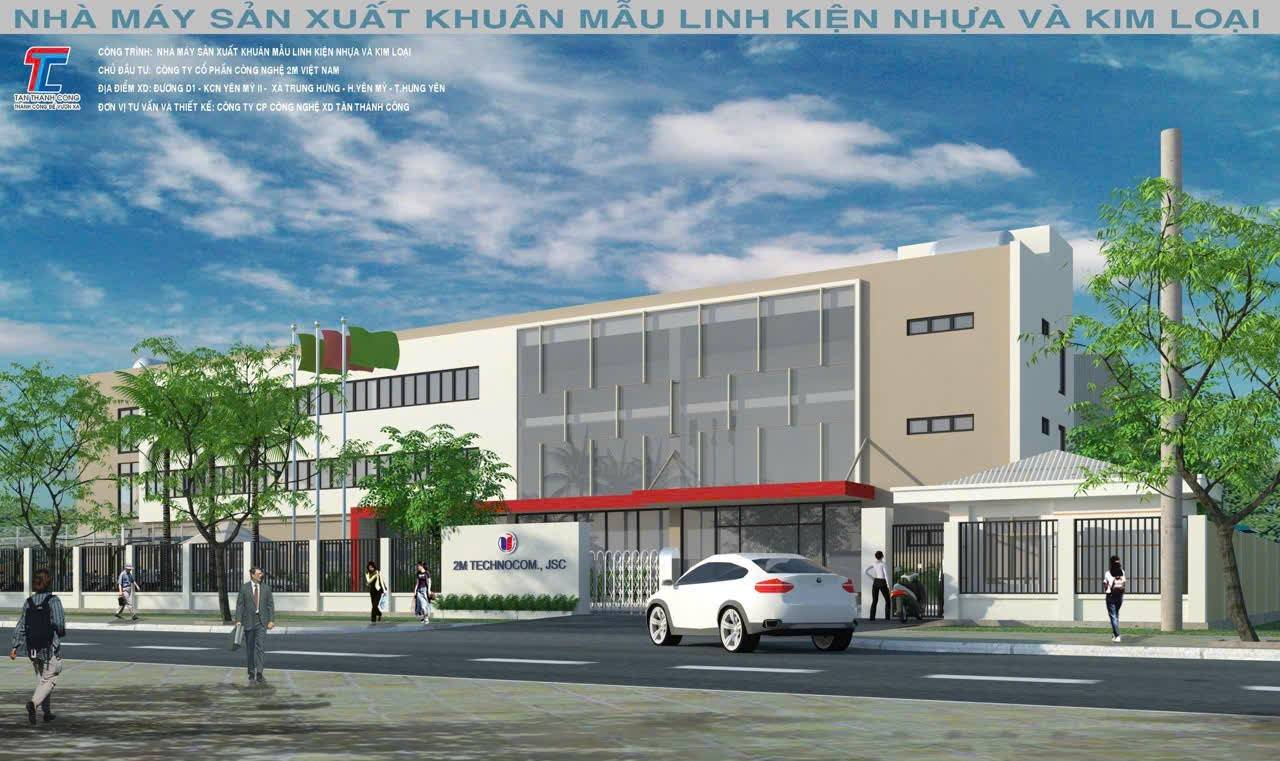
\includegraphics[width=70mm,height=46mm]{../../public/project-assets/2m1.jpg}};
    \fill[TTCDeepNavy,opacity=.88] (0,174) rectangle (70,185);
    \node[anchor=west,text=white,font=\fontsize{7}{8}\selectfont\bfseries]
      at (4,179.5) {DESIGN PERSPECTIVE};
  \end{scope}
  \begin{scope}
    \clip[rounded corners=2pt] (0,150) rectangle (34,172);
    \node[inner sep=0pt] at (17,161)
      {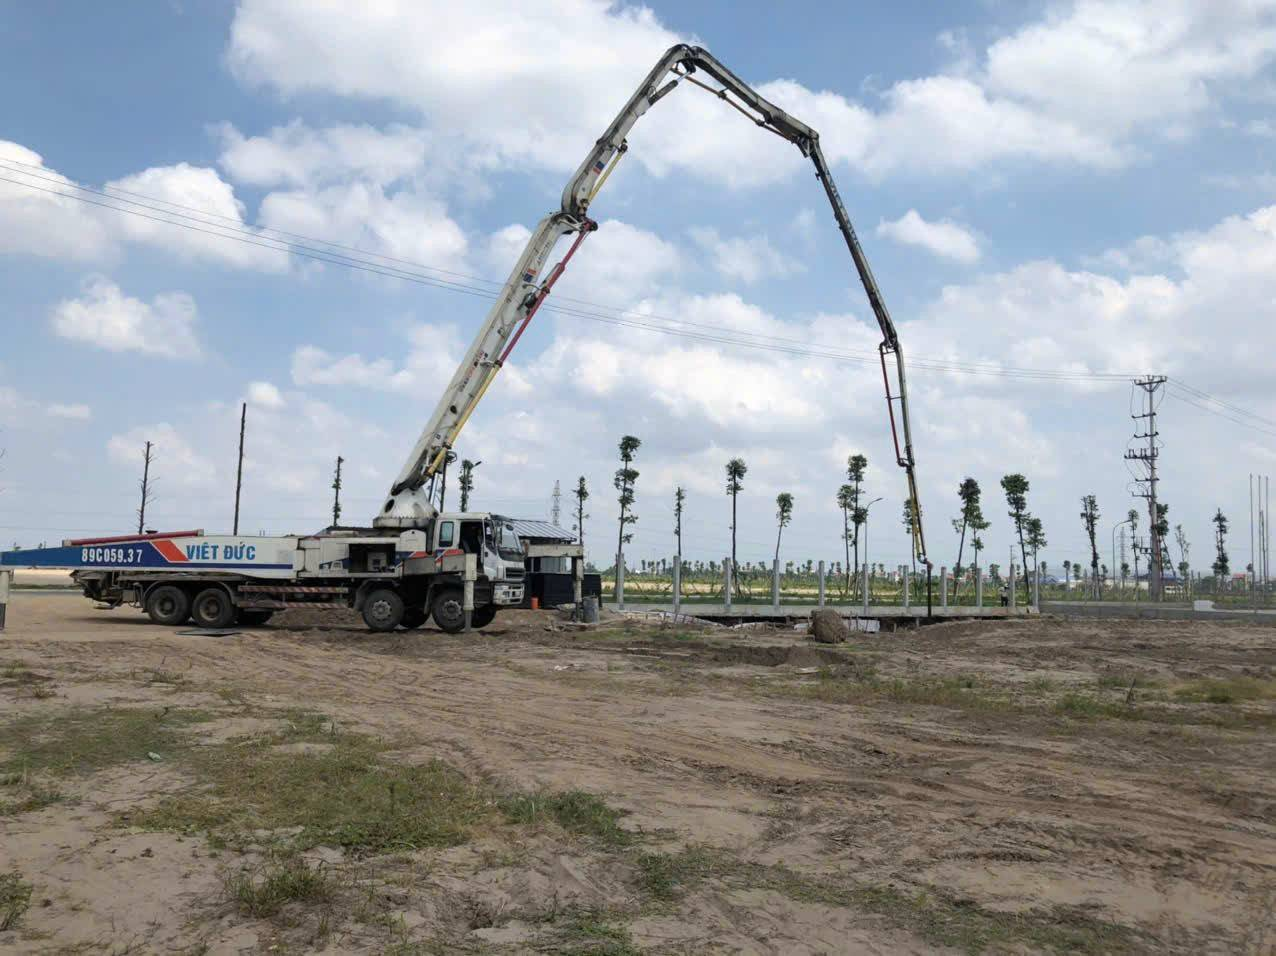
\includegraphics[width=34mm,height=22mm]{../../public/project-assets/2m3.jpg}};
  \end{scope}
  \begin{scope}
    \clip[rounded corners=2pt] (36,150) rectangle (70,172);
    \node[inner sep=0pt] at (53,161)
      {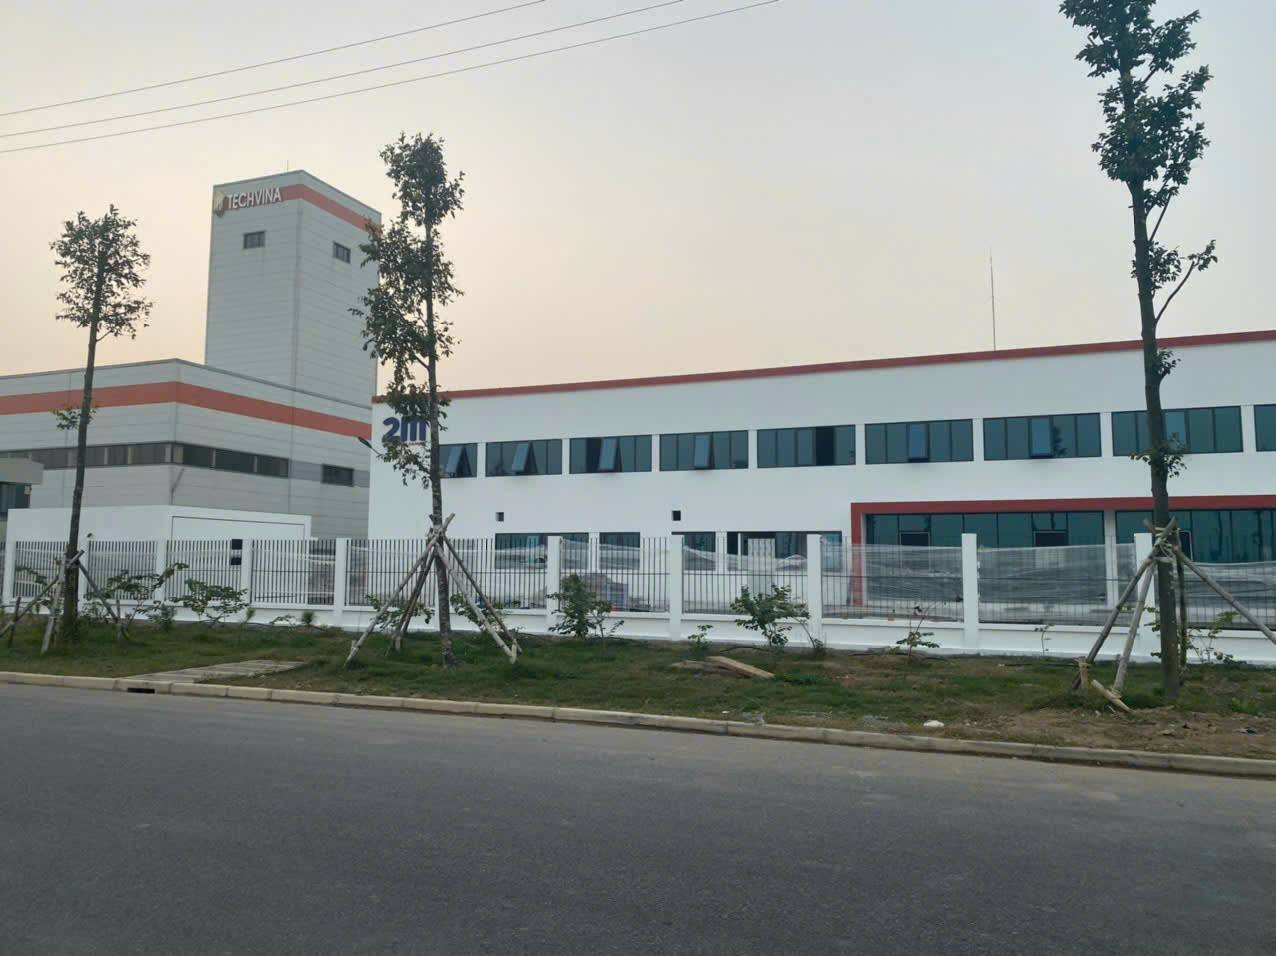
\includegraphics[width=34mm,height=22mm]{../../public/project-assets/2m5.jpg}};
  \end{scope}
  \fill[TTCDeepNavy,opacity=.82] (0,150) rectangle (34,156);
  \fill[TTCDeepNavy,opacity=.82] (36,150) rectangle (70,156);
  \node[anchor=west,text=white,font=\fontsize{4.8}{5.6}\selectfont\bfseries] at (2,153) {CONSTRUCTION PHOTOS};
  \node[anchor=west,text=white,font=\fontsize{4.8}{5.6}\selectfont\bfseries] at (38,153) {FINISHED PHOTO};
  \draw[TTCBorder,rounded corners=4pt,line width=.7pt] (0,150) rectangle (70,220);

  % Tóm tắt điều hành
  \fill[TTCLightBlue,rounded corners=4pt] (74,150) rectangle (186,220);
  \draw[TTCBorder,rounded corners=4pt,line width=.7pt] (74,150) rectangle (186,220);
  \node[anchor=north west,text=TTCRed,font=\fontsize{7.5}{9}\selectfont\bfseries]
    at (80,214) {DESIGN CONSULTANCY \& GENERAL CONTRACTOR};
  \node[anchor=north west,text width=99mm,align=left,text=TTCBlue,
        font=\fontsize{13}{15}\selectfont\bfseries]
    at (80,207) {2M TECHNOLOGY FACTORY COMPLEX};
  \draw[TTCBorder,line width=.55pt] (80,190) -- (180,190);
  \foreach \x in {113.3,146.6}{\draw[TTCBorder,line width=.5pt] (\x,163) -- (\x,186);}
  \node[align=center,text width=29mm] at (96.5,176) {
    {\fontsize{9.5}{11}\selectfont\bfseries\color{TTCRed}PRECISION MECHANICS}\\[-.5mm]
    {\fontsize{6.2}{7.4}\selectfont\color{TTCTextMuted}PATTERN \& PLASTIC}};
  \node[align=center,text width=29mm] at (130,176) {
    {\fontsize{9.5}{11}\selectfont\bfseries\color{TTCBlue}STEEL STRUCTURE}\\[-.5mm]
    {\fontsize{6.2}{7.4}\selectfont\color{TTCTextMuted}WORKSHOP \& 3-STOREY OFFICE}};
  \node[align=center,text width=29mm] at (163.5,176) {
    {\fontsize{9.5}{11}\selectfont\bfseries\color{TTCBlue}ANTI-VIBRATION}\\[-.5mm]
    {\fontsize{6.2}{7.4}\selectfont\color{TTCTextMuted}FOR CNC MACHINE SETS}};
  \node[anchor=south west,text width=99mm,align=left,text=TTCTextDark,
        font=\fontsize{7.4}{9}\selectfont]
    at (80,153) {\textbf{Client:} 2M Vietnam Technology Joint Stock Company (2M TECHNOCOM., JSC) \textbullet\ \textbf{Implementing unit:} Tan Thanh Cong JSC -- steel structure design, construction consultancy, bearing floor and technical infrastructure.};

  % Câu chuyện dự án: bài toán -- giải pháp -- kết quả
  \node[anchor=west,text=TTCBlue,font=\fontsize{8}{9.5}\selectfont\bfseries]
    at (0,143) {PROJECT STORY • ONLY KEEP THE THREE MAIN POINTS};

  \fill[white,rounded corners=4pt] (0,79) rectangle (58,137);
  \draw[TTCBorder,rounded corners=4pt,line width=.7pt] (0,79) rectangle (58,137);
  \fill[TTCRed,rounded corners=2pt] (5,124) rectangle (16,133);
  \node[text=white,font=\fontsize{7}{8}\selectfont\bfseries] at (10.5,128.5) {01};
  \node[anchor=north west,text=TTCBlue,font=\fontsize{9}{10.5}\selectfont\bfseries]
    at (5,120) {PROBLEM};
  \node[anchor=north west,text width=48mm,align=left,text=TTCTextDark,
        font=\fontsize{7.2}{9}\selectfont]
    at (5,110) {Client needs to build a factory to produce high-precision molds and technical components, requiring a stable anti-vibration workshop floor for CNC machines \& plastic injection molding machine.};

  \draw[-{Latex[length=2.5mm]},TTCCyan,line width=1pt] (59.5,108) -- (63,108);
  \fill[TTCDeepNavy,rounded corners=4pt] (64,79) rectangle (122,137);
  \node[text=TTCDeepNavy,fill=white,rounded corners=2pt,font=\fontsize{7}{8}\selectfont\bfseries,
        minimum width=11mm,minimum height=9mm] at (74.5,128.5) {02};
  \node[anchor=north west,text=white,font=\fontsize{9}{10.5}\selectfont\bfseries]
    at (69,120) {TTC SOLUTIONS};
  \node[anchor=north west,text width=48mm,align=left,text=white,
        font=\fontsize{7.2}{9}\selectfont]
    at (69,110) {Consulting on optimal design of ventilated workshop rhythm; strengthening the foundation \& the concrete floor is subjected to anti-vibration load; synchronous integration of MEP system, lighting and transformer station of the industrial park.};

  \draw[-{Latex[length=2.5mm]},TTCCyan,line width=1pt] (123.5,108) -- (127,108);
  \fill[TTCLightBlue,rounded corners=4pt] (128,79) rectangle (186,137);
  \draw[TTCBorder,rounded corners=4pt,line width=.7pt] (128,79) rectangle (186,137);
  \fill[TTCBlue,rounded corners=2pt] (133,124) rectangle (144,133);
  \node[text=white,font=\fontsize{7}{8}\selectfont\bfseries] at (138.5,128.5) {03};
  \node[anchor=north west,text=TTCBlue,font=\fontsize{9}{10.5}\selectfont\bfseries]
    at (133,120) {RESULTS};
  \node[anchor=north west,text width=48mm,align=left,text=TTCTextDark,
        font=\fontsize{7.2}{9}\selectfont]
    at (133,110) {Handing over the completed works in accordance with schedule, meeting the strict technical standards of the high-tech mold manufacturing industry, putting them into effective operation.};

  % Băng ghi nhớ
  \fill[white,rounded corners=4pt] (0,20) rectangle (186,70);
  \draw[TTCBorder,rounded corners=4pt,line width=.7pt] (0,20) rectangle (186,70);
  \node[anchor=west,text=TTCBlue,font=\fontsize{8}{9.5}\selectfont\bfseries]
    at (7,61) {THREE POINTS FOR READERS TO REMEMBER};
  \draw[TTCBorder] (62,27) -- (62,58);
  \draw[TTCBorder] (124,27) -- (124,58);
  \node[align=center,text width=52mm] at (31,42) {
    {\fontsize{11}{12}\selectfont\bfseries\color{TTCRed}ANTI-VIBRATION}\\[-.5mm]
    {\fontsize{6.6}{8}\selectfont\color{TTCTextMuted}REINFORCED FLOOR FOR CNC MACHINE SETS}};
  \node[align=center,text width=52mm] at (93,42) {
    {\fontsize{11}{12}\selectfont\bfseries\color{TTCBlue}PACKAGE GENERAL CONTRACTOR}\\[-.5mm]
    {\fontsize{6.6}{8}\selectfont\color{TTCTextMuted}DESIGN CONSULTANCY • STRUCTURE • MEP}};
  \node[align=center,text width=52mm] at (155,42) {
    {\fontsize{11}{12}\selectfont\bfseries\color{TTCBlue}BENCHMARK PROGRESS}\\[-.5mm]
    {\fontsize{6.6}{8}\selectfont\color{TTCTextMuted}TURNKEY HANDOVER}};

  \fill[TTCDeepNavy,rounded corners=3pt] (0,0) rectangle (186,14);
  \node[anchor=west,text=white,font=\fontsize{7.4}{9}\selectfont\bfseries]
    at (7,7) {CORE VALUES: PRECISION TECHNOLOGY SPACE • COMPREHENSIVE GENERAL CONTRACTOR PACKAGE};
\end{tikzpicture}
\end{minipage}
\newpage

% ============================================================
% PAGE 23: ENGINEERING CASE -- NHÀ MÁY SƠN ALO VIỆT NAM
% ============================================================
\noindent\mbox{}\par\vspace{-\baselineskip}
\casepagebars{ENGINEERING SOLUTION • ALO PAINT FACTORY}{Page 23}

\begin{minipage}[t][246mm]{\textwidth}
\secbrand{Project Profile 02: Manufacturing Plant ALO Paint Vietnam}{Chemical \& Paint manufacturing complex • ATEX standard fire prevention and fighting • Phu Nghia Industrial Park, Hanoi}

\noindent
\begin{tikzpicture}[x=1mm,y=1mm]
  \path[use as bounding box] (0,0) rectangle (186,220);

  % Phối cảnh và thẻ dữ liệu
  \begin{scope}
    \clip[rounded corners=4pt] (0,148) rectangle (104,220);
    \node[inner sep=0pt] at (52,184)
      {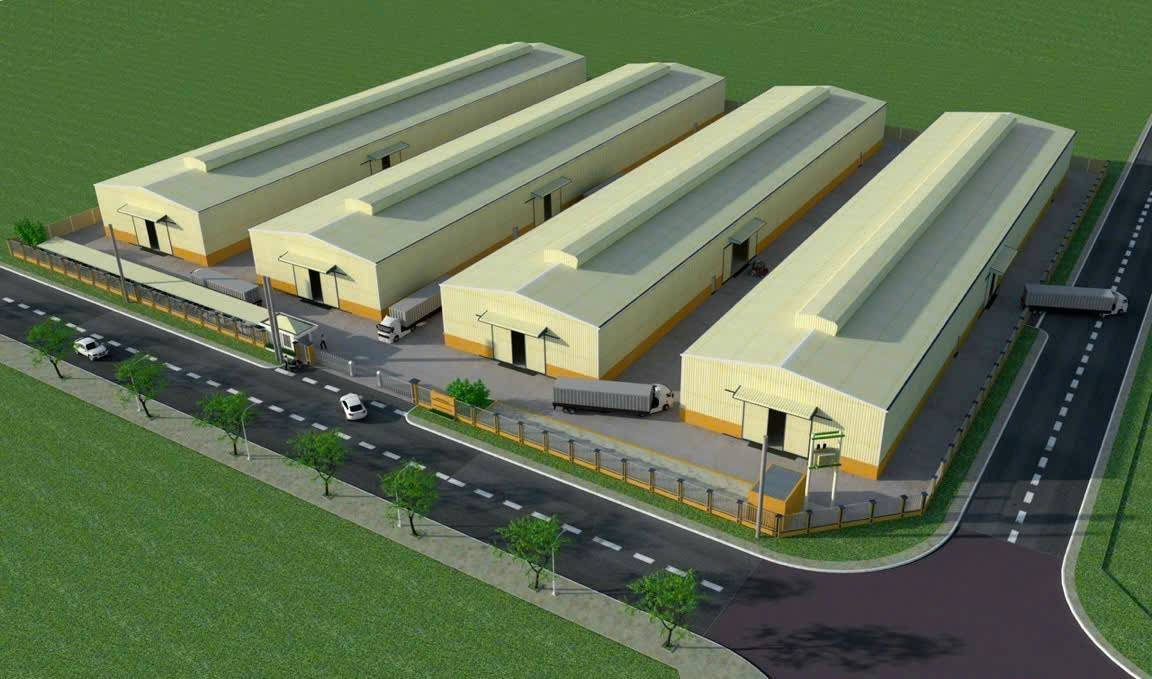
\includegraphics[width=104mm,height=77.5mm]{../../public/project-assets/son_alo_2.jpg}};
    \fill[TTCDeepNavy,opacity=.88] (0,148) rectangle (104,160);
    \node[anchor=west,text=white,font=\fontsize{7}{8}\selectfont\bfseries]
      at (4,154) {OVERALL PERSPECTIVE • PHU NGHIA IP, HANOI};
  \end{scope}
  % Ảnh thực tế tại mốc khởi công, trình bày như bằng chứng tiến trình
  \begin{scope}
    \clip[rounded corners=2pt] (73,181) rectangle (101,217);
    \node[inner sep=0pt] at (87,199)
      {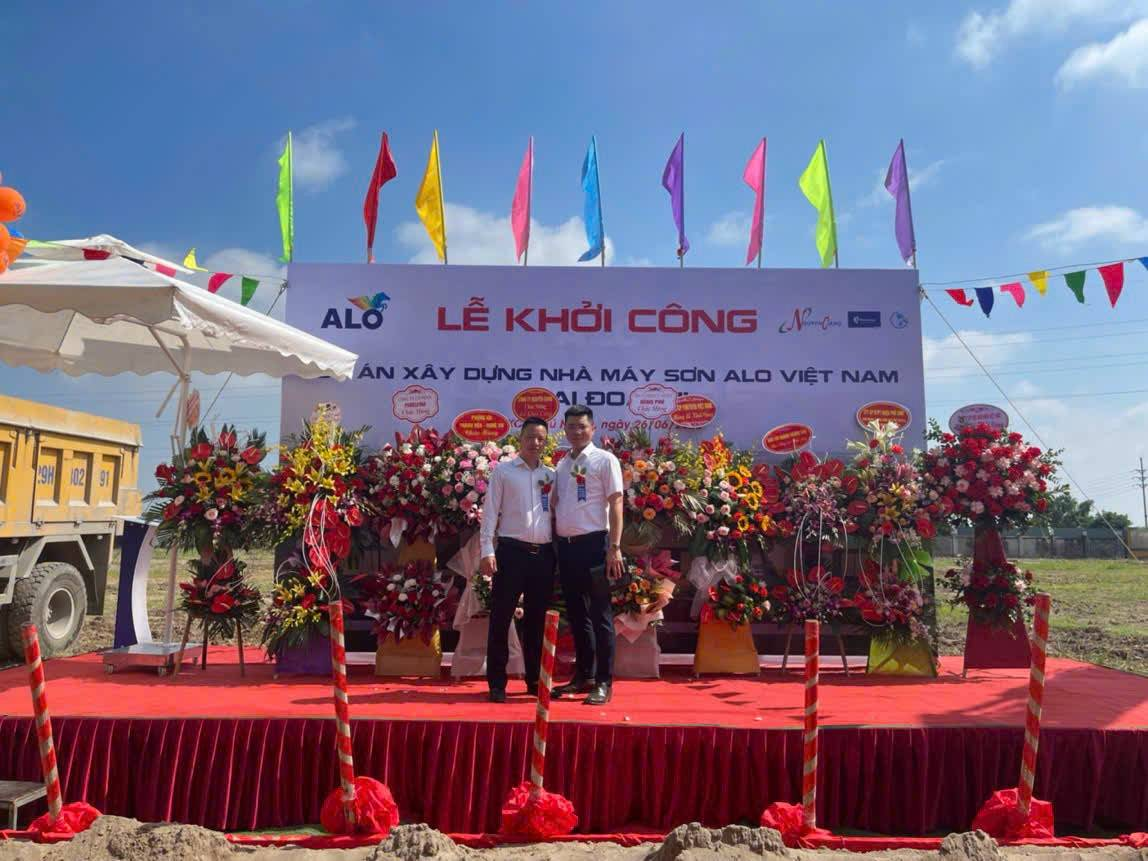
\includegraphics[width=28mm,height=36mm]{../../public/project-assets/son_alo_1.jpg}};
  \end{scope}
  \draw[white,line width=1.2pt,rounded corners=2pt] (73,181) rectangle (101,217);
  \fill[TTCDeepNavy,opacity=.88] (73,181) rectangle (101,188);
  \node[anchor=west,text=white,font=\fontsize{4.7}{5.5}\selectfont\bfseries]
    at (75,184.5) {PHOTO OF COMMENCEMENT CEREMONY};
  \draw[TTCBorder,rounded corners=4pt,line width=.7pt] (0,148) rectangle (104,220);

  \fill[TTCDeepNavy,rounded corners=4pt] (108,148) rectangle (186,220);
  \node[anchor=north west,text=TTCCyan,font=\fontsize{7.2}{8.5}\selectfont\bfseries]
    at (114,214) {EPC GENERAL CONTRACTOR};
  \node[anchor=north west,text=white,font=\fontsize{13.5}{15}\selectfont\bfseries]
    at (114,206) {ALO PAINT COMBINATION};
  \node[anchor=north west,text=white!75!gray,font=\fontsize{6.5}{8}\selectfont]
    at (114,192) {CLUSTER OF 4 WORKSHOPS \& CHEMICAL STORAGE};
  \draw[white!25!gray] (114,184) -- (180,184);
  \node[anchor=north west,text width=66mm,align=left,text=white,
        font=\fontsize{7.2}{9}\selectfont]
    at (114,179) {\textbf{Client:} ALO Vietnam Investment Joint Stock Company\\[1mm]
                  \textbf{Location:} Lot CN1, Phu Nghia Industrial Park, Hanoi\\[1mm]
                  \textbf{Standard (s):} Fire safety \& Chemical resistance\\[1mm]
                  \textbf{Tan Thanh Cong JSC:} EPC General Contractor (Design \& Construction)};

  % Sơ đồ kỹ thuật: Nhà xưởng hóa chất sơn & kiểm soát môi trường
  \node[anchor=west,text=TTCBlue,font=\fontsize{8}{9.5}\selectfont\bfseries]
    at (0,140) {PRINCIPLE DIAGRAM • SAFETY SOLUTION WITH FULL EXPLOSION \& CHEMICAL RESISTANCE};
  \fill[TTCLightBlue,rounded corners=4pt] (0,53) rectangle (186,134);
  \draw[TTCBorder,rounded corners=4pt,line width=.7pt] (0,53) rectangle (186,134);

  % Bản vẽ sơ đồ phân xưởng hóa chất
  % Mái dốc + Cửa trời thông gió
  \draw[TTCBlue,line width=1.4pt] (12,118) -- (68,126) -- (128,118);
  \draw[TTCRed,line width=1pt] (58,126) -- (58,130) -- (78,130) -- (78,126);
  \node[anchor=south,text=TTCRed,font=\fontsize{5.8}{7}\selectfont\bfseries] at (68,130.5) {SOLVENT VAPOR OUTLET};

  % Khung cột thép
  \draw[TTCBlue,line width=1.4pt] (12,67) -- (12,118);
  \draw[TTCBlue,line width=1.4pt] (128,67) -- (128,118);
  \foreach \x in {41,70,99}{
    \draw[TTCBlue,line width=1pt,dashed] (\x,67) -- (\x,122);
  }

  % Tuyến PCCC Sprinkler & Foam
  \draw[TTCRed,line width=1.2pt,dashed] (15,108) -- (125,108);
  \foreach \x in {25,50,75,100,120}{
    \fill[TTCRed] (\x,108) circle (1.2mm);
    \draw[-{Latex[length=1.5mm]},TTCRed,line width=.6pt] (\x,106) -- (\x,100);
  }
  \node[anchor=west,text=TTCRed,font=\fontsize{6.3}{7.5}\selectfont\bfseries]
    at (16,112) {FOAM AUTOMATIC FIRE NETWORK \& SPRINKLER};

  % Bồn khuấy & Dây chuyền sản xuất
  \fill[white] (22,72) rectangle (40,94);
  \draw[TTCBorder,line width=.7pt] (22,72) rectangle (40,94);
  \node[align=center,text=TTCBlue,font=\fontsize{6}{7.2}\selectfont\bfseries] at (31,83) {STIRRING TANK\\PHA SON NATIONAL PARK};

  \fill[white] (50,72) rectangle (72,94);
  \draw[TTCBorder,line width=.7pt] (50,72) rectangle (72,94);
  \node[align=center,text=TTCBlue,font=\fontsize{6}{7.2}\selectfont\bfseries] at (61,83) {LINES\\PACKAGING};

  \fill[white] (82,72) rectangle (120,94);
  \draw[TTCBorder,line width=.7pt] (82,72) rectangle (120,94);
  \node[align=center,text=TTCBlue,font=\fontsize{6}{7.2}\selectfont\bfseries] at (101,83) {FINISHED GOODS WAREHOUSE \&\\CHEMICAL RAW MATERIALS};

  % Sàn Epoxy
  \fill[TTCDeepNavy!85!black] (10,64) rectangle (130,68);
  \node[anchor=north west,text=TTCDeepNavy,font=\fontsize{6.2}{7.5}\selectfont\bfseries]
    at (12,63) {EPOXY SELF-LEVELING CONCRETE FLOOR WITH CHEMICAL RESISTANCE};

  % Chú giải bên phải
  \draw[TTCBorder] (136,58) -- (136,128);
  \node[anchor=north west,text=TTCBlue,font=\fontsize{7.2}{8.5}\selectfont\bfseries]
    at (141,126) {3 TECHNICAL DECISIONS};
  \node[anchor=north west,text width=40mm,align=left,text=TTCTextDark,
        font=\fontsize{6.5}{8.1}\selectfont]
    at (141,117) {\textbf{01 • Chemical resistance}\newline
                  Epoxy-coated composite concrete floor is resistant to organic solvents.};
  \node[anchor=north west,text width=40mm,align=left,text=TTCTextDark,
        font=\fontsize{6.5}{8.1}\selectfont]
    at (141,94) {\textbf{02 • Fire safety}\newline
                  Rockwool fire retardant wall, Foam system \& fire alarm according to the approved dossier.};
  \node[anchor=north west,text width=40mm,align=left,text=TTCTextDark,
        font=\fontsize{6.5}{8.1}\selectfont]
    at (141,71) {\textbf{03 • Microclimate ventilation}\newline
                  Natural gas convection louvers continuously release solvent vapor concentrations.};

  % Ba ý ghi nhớ
  \fill[white,rounded corners=3pt] (0,20) rectangle (58,52);
  \draw[TTCBorder,rounded corners=3pt,line width=.7pt] (0,20) rectangle (58,52);
  \node[anchor=north west,text=TTCRed,font=\fontsize{8}{9}\selectfont\bfseries]
    at (5,47) {01 • DEDICATED FIRE PROTECTION};
  \node[anchor=north west,text width=48mm,text=TTCTextDark,font=\fontsize{6.8}{8.4}\selectfont]
    at (5,38) {Foam fire fighting system and solutions to prevent fire spread according to approved documents.};

  \fill[white,rounded corners=3pt] (64,20) rectangle (122,52);
  \draw[TTCBorder,rounded corners=3pt,line width=.7pt] (64,20) rectangle (122,52);
  \node[anchor=north west,text=TTCBlue,font=\fontsize{8}{9}\selectfont\bfseries]
    at (69,47) {02 • CORROSION RESISTANT FLOOR};
  \node[anchor=north west,text width=48mm,text=TTCTextDark,font=\fontsize{6.8}{8.4}\selectfont]
    at (69,38) {Epoxy-coated reinforced concrete is resistant to solvents and chemicals according to operating requirements.};

  \fill[white,rounded corners=3pt] (128,20) rectangle (186,52);
  \draw[TTCBorder,rounded corners=3pt,line width=.7pt] (128,20) rectangle (186,52);
  \node[anchor=north west,text=TTCBlue,font=\fontsize{8}{9}\selectfont\bfseries]
    at (133,47) {03 • EPC PROGRESS};
  \node[anchor=north west,text width=48mm,text=TTCTextDark,font=\fontsize{6.8}{8.4}\selectfont]
    at (133,38) {Handing over the synchronous package of production workshops, warehouses and operating areas.};

  \fill[TTCDeepNavy,rounded corners=3pt] (0,0) rectangle (186,14);
  \node[anchor=west,text=white,font=\fontsize{7.4}{9}\selectfont\bfseries]
    at (7,7) {CORE VALUES: SAFETY FULL CHEMICAL EXPLOSION • DURABLE FLOOR CORROSION RESISTANCE};
\end{tikzpicture}
\end{minipage}
\newpage

% ============================================================
% PAGE 24: INJECTION MOLDING CASE -- NHÀ MÁY NHỰA SENDAI VIỆT NAM
% ============================================================
\noindent\mbox{}\par\vspace{-\baselineskip}
\casepagebars{ENGINEERING SOLUTION • SENDAI PLASTICS FACTORY}{Page 24}

\begin{minipage}[t][246mm]{\textwidth}
\secbrand{Project Profile 03: Manufacturing Plant Sendai Plastic Vietnam}{High-tech plastics manufacturing plant • Injection molding facility • Industrial Park No. 3, Hung Yen}

\noindent
\begin{tikzpicture}[x=1mm,y=1mm]
  \path[use as bounding box] (0,0) rectangle (186,220);

  % Phối cảnh và thẻ dữ liệu
  \begin{scope}
    \clip[rounded corners=4pt] (0,148) rectangle (104,220);
    \node[inner sep=0pt] at (52,184)
      {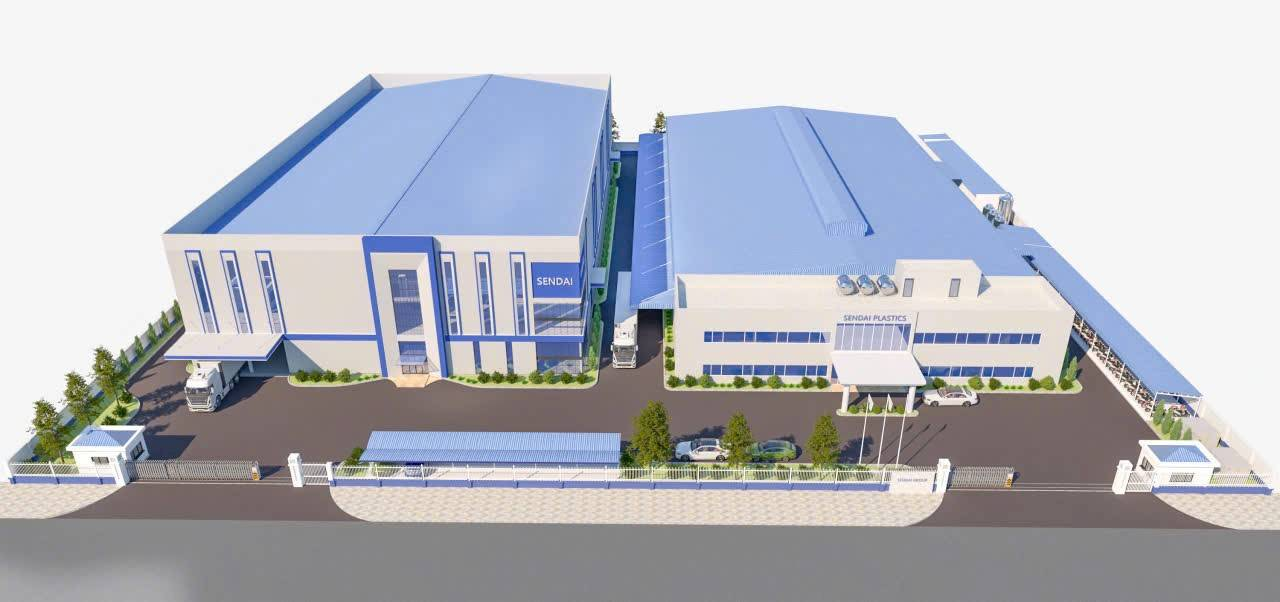
\includegraphics[width=104mm,height=77.5mm]{../../public/project-assets/sendai_1.jpg}};
    \fill[TTCDeepNavy,opacity=.88] (0,148) rectangle (104,160);
    \node[anchor=west,text=white,font=\fontsize{7}{8}\selectfont\bfseries]
      at (4,154) {OVERALL PERSPECTIVE • INDUSTRIAL PARK NO. 03, HUNG YEN};
  \end{scope}
  % Không có ảnh hiện trường trong bộ nguồn: dùng góc phối cảnh thứ hai và ghi nhãn rõ
  \begin{scope}
    \clip[rounded corners=2pt] (68,190) rectangle (101,216);
    \node[inner sep=0pt] at (84.5,203)
      {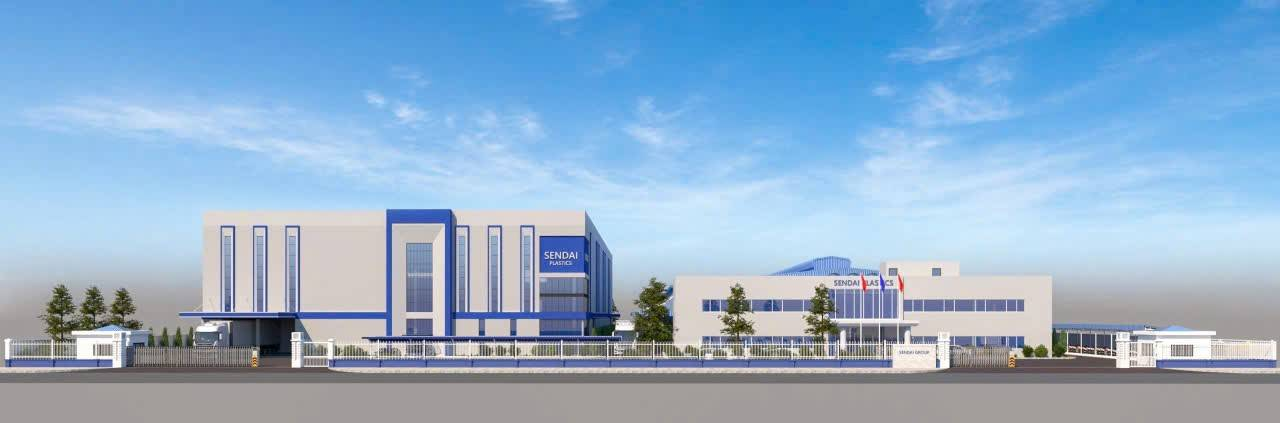
\includegraphics[width=50mm,height=26mm]{../../public/project-assets/sendai_3.jpg}};
  \end{scope}
  \draw[white,line width=1.2pt,rounded corners=2pt] (68,190) rectangle (101,216);
  \fill[TTCDeepNavy,opacity=.88] (68,190) rectangle (101,197);
  \node[anchor=west,text=white,font=\fontsize{4.6}{5.4}\selectfont\bfseries]
    at (70,193.5) {PERSPECTIVE};
  \draw[TTCBorder,rounded corners=4pt,line width=.7pt] (0,148) rectangle (104,220);

  \fill[TTCDeepNavy,rounded corners=4pt] (108,148) rectangle (186,220);
  \node[anchor=north west,text=TTCCyan,font=\fontsize{7.2}{8.5}\selectfont\bfseries]
    at (114,214) {GENERAL CONTRACTOR};
  \node[anchor=north west,text=white,font=\fontsize{13.5}{15}\selectfont\bfseries]
    at (114,206) {SENDAI PLASTIC ASSEMBLY};
  \node[anchor=north west,text=white!75!gray,font=\fontsize{6.5}{8}\selectfont]
    at (114,192) {CLUSTER OF 2 WORKSHOPS \& OFFICE BLOCK};
  \draw[white!25!gray] (114,184) -- (180,184);
  \node[anchor=north west,text width=66mm,align=left,text=white,
        font=\fontsize{7.2}{9}\selectfont]
    at (114,179) {\textbf{Client:} Sendai Vietnam Plastic Joint Stock Company\\[1mm]
                  \textbf{Location:} Lot C7, Industrial Park No. 3, An Thi, Hung Yen\\[1mm]
                  \textbf{Scale:} 2 Extrusion workshop \& 3-storey office building\\[1mm]
                  \textbf{Tan Thanh Cong JSC:} General contractor for construction \& MEP};

  % Sơ đồ kỹ thuật: Nhà xưởng đúc ép nhựa & mạng lưới phụ trợ MEP
  \node[anchor=west,text=TTCBlue,font=\fontsize{8}{9.5}\selectfont\bfseries]
    at (0,140) {PRINCIPLE DIAGRAM • PLASTIC INJECTION MOLDING LINE \& MEP BACKEND SYSTEM};
  \fill[TTCLightBlue,rounded corners=4pt] (0,53) rectangle (186,134);
  \draw[TTCBorder,rounded corners=4pt,line width=.7pt] (0,53) rectangle (186,134);

  % Bản vẽ sơ đồ phân xưởng đúc ép
  % Mái dốc kết cấu thép PEB
  \draw[TTCBlue,line width=1.4pt] (12,122) -- (68,130) -- (128,122);

  % Khung cột thép
  \draw[TTCBlue,line width=1.4pt] (12,67) -- (12,122);
  \draw[TTCBlue,line width=1.4pt] (128,67) -- (128,122);
  \foreach \x in {41,70,99}{
    \draw[TTCBlue,line width=1pt,dashed] (\x,67) -- (\x,125);
  }

  % Dầm cầu trục chạy trên cao (Overhead Crane)
  \draw[TTCRed,line width=1.4pt] (14,112) -- (126,112);
  \fill[TTCRed] (44,110) rectangle (58,114);
  \node[anchor=south,text=TTCRed,font=\fontsize{5.8}{7}\selectfont\bfseries] at (51,114.8) {CRANE FOR MOULD REPLACEMENT};
  \draw[-{Latex[length=1.5mm]},TTCRed,line width=.8pt] (51,110) -- (51,96);

  % Tuyến đường ống Chiller / Nước giải nhiệt & Khí nén
  \draw[TTCCyan,line width=1.2pt,dashed] (15,102) -- (125,102);
  \node[anchor=west,text=TTCCyan,font=\fontsize{6.3}{7.5}\selectfont\bfseries]
    at (16,105) {MOLD COOLING CHILLER PIPING \& MEDIUM COMPRESSED AIR DEDICATION};

  % Cụm máy ép phun thủy lực (Injection Molding Machines)
  \foreach \x/\label in {20/{PRESS 01\\350 TONS}, 56/{PRESS 02\\650 TONS}, 92/{PRESS 03\\850 TONS}}{
    \fill[white] (\x,72) rectangle +(28,22);
    \draw[TTCBorder,line width=.7pt] (\x,72) rectangle +(28,22);
    \node[align=center,text=TTCBlue,font=\fontsize{6}{7.2}\selectfont\bfseries] at (\x+14,83) {\label};
    % Mũi tên cấp Chiller
    \draw[-{Latex[length=1.2mm]},TTCCyan,line width=.6pt] (\x+14,102) -- (\x+14,94);
  }

  % Sàn bê tông gia cường chịu tải máy ép
  \fill[TTCDeepNavy!85!black] (10,64) rectangle (130,68);
  \node[anchor=north west,text=TTCDeepNavy,font=\fontsize{6.2}{7.5}\selectfont\bfseries]
    at (12,63) {PRESS CYCLE ANTI-VIBRATION REINFORCED CONCRETE FLOOR};

  % Chú giải bên phải
  \draw[TTCBorder] (136,58) -- (136,128);
  \node[anchor=north west,text=TTCBlue,font=\fontsize{7.2}{8.5}\selectfont\bfseries]
    at (141,126) {3 TECHNICAL DECISIONS};
  \node[anchor=north west,text width=40mm,align=left,text=TTCTextDark,
        font=\fontsize{6.5}{8.1}\selectfont]
    at (141,117) {\textbf{01 • Press-loaded floor}\newline
                  High-grade reinforced concrete prevents misalignment settlement and suppresses machine vibration.};
  \node[anchor=north west,text width=40mm,align=left,text=TTCTextDark,
        font=\fontsize{6.5}{8.1}\selectfont]
    at (141,94) {\textbf{02 • Chiller Infrastructure}\newline
                  Closed circulating cooling water network feeds directly to each mold.};
  \node[anchor=north west,text width=40mm,align=left,text=TTCTextDark,
        font=\fontsize{6.5}{8.1}\selectfont]
    at (141,71) {\textbf{03 • Complex of 2 workshops \& VP}\newline
                  Internal traffic planning connects smoothly between the workshop and the operation.};

  % Ba ý ghi nhớ
  \fill[white,rounded corners=3pt] (0,20) rectangle (58,52);
  \draw[TTCBorder,rounded corners=3pt,line width=.7pt] (0,20) rectangle (58,52);
  \node[anchor=north west,text=TTCRed,font=\fontsize{8}{9}\selectfont\bfseries]
    at (5,47) {01 • TECHNICAL INJECTION MOLDING};
  \node[anchor=north west,text width=48mm,text=TTCTextDark,font=\fontsize{6.8}{8.4}\selectfont]
    at (5,38) {The large aperture workshop integrates the crane to replace the mold according to the equipment data.};

  \fill[white,rounded corners=3pt] (64,20) rectangle (122,52);
  \draw[TTCBorder,rounded corners=3pt,line width=.7pt] (64,20) rectangle (122,52);
  \node[anchor=north west,text=TTCBlue,font=\fontsize{8}{9}\selectfont\bfseries]
    at (69,47) {02 • MEP COOLING};
  \node[anchor=north west,text width=48mm,text=TTCTextDark,font=\fontsize{6.8}{8.4}\selectfont]
    at (69,38) {Cooling chiller system, central compressed air and synchronous power station.};

  \fill[white,rounded corners=3pt] (128,20) rectangle (186,52);
  \draw[TTCBorder,rounded corners=3pt,line width=.7pt] (128,20) rectangle (186,52);
  \node[anchor=north west,text=TTCBlue,font=\fontsize{8}{9}\selectfont\bfseries]
    at (133,47) {03 • PROGRESS OF GENERAL CONTRACTOR};
  \node[anchor=north west,text width=48mm,text=TTCTextDark,font=\fontsize{6.8}{8.4}\selectfont]
    at (133,38) {Package construction of 2 production workshops, warehouse and 3-storey office block.};

  \fill[TTCDeepNavy,rounded corners=3pt] (0,0) rectangle (186,14);
  \node[anchor=west,text=white,font=\fontsize{7.4}{9}\selectfont\bfseries]
    at (7,7) {CORE VALUES: TECHNICAL PLASTIC PRODUCTION INFRASTRUCTURE • SYNCHRONOUS MEP AUXILIARY SYSTEM};
\end{tikzpicture}
\end{minipage}
\newpage

% ============================================================
% PAGE 25: CASE STUDY 04 -- NHÀ MÁY MAY LÀO CAI
% ============================================================
\noindent\mbox{}\par\vspace{-\baselineskip}
\casepagebars{ENGINEERING SOLUTION • LAO CAI GARMENT FACTORY}{Page 25}

\begin{minipage}[t][246mm]{\textwidth}
\secbrand{Project Profile 04: Factory Complex Lao Cai}{Multi-storey garment manufacturing complex • Negative pressure cooling • New Street, Lao Cai City}

\noindent
\begin{tikzpicture}[x=1mm,y=1mm]
  \path[use as bounding box] (0,0) rectangle (186,220);

  % Phối cảnh dự án (trái)
  \begin{scope}
    \clip[rounded corners=4pt] (0,148) rectangle (104,220);
    \node[inner sep=0pt] at (52,175)
      {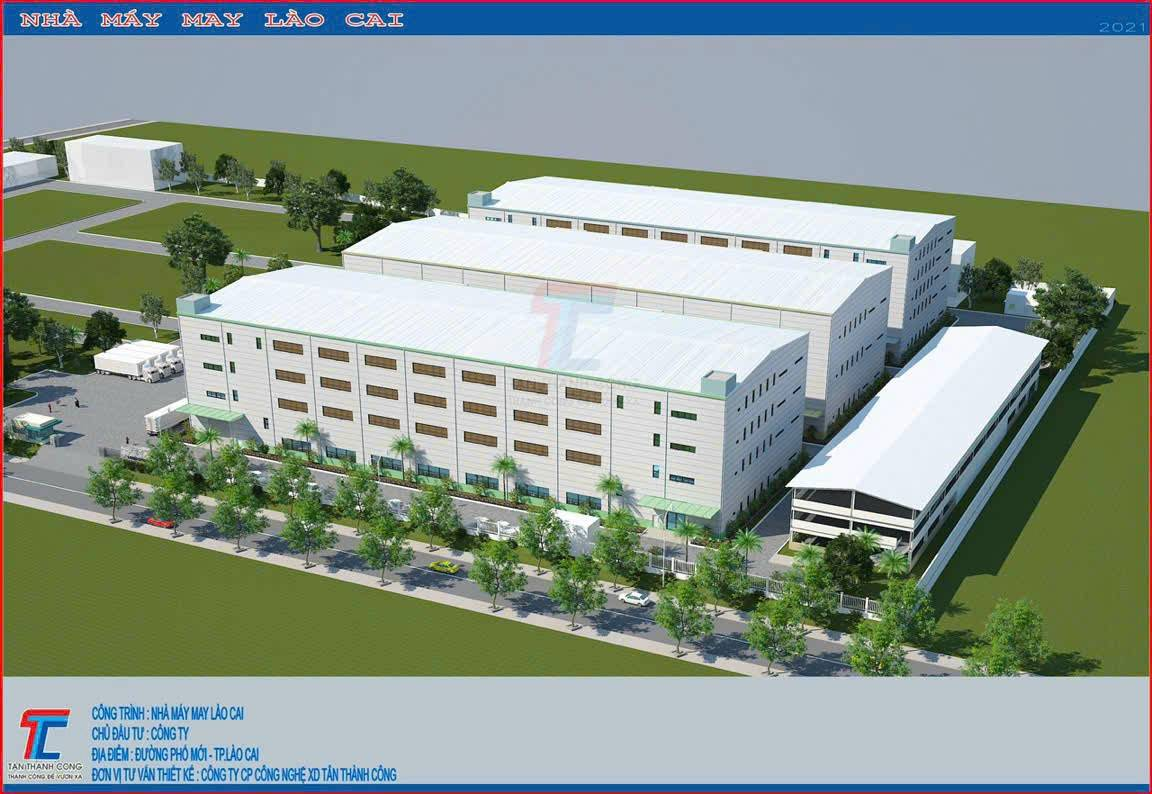
\includegraphics[width=128mm]{../../public/project-assets/laocai_4.jpg}};
    \fill[TTCDeepNavy,opacity=.92] (0,148) rectangle (104,158);
    \node[anchor=west,text=white,font=\fontsize{6.8}{8}\selectfont\bfseries]
      at (4,153) {OVERALL PERSPECTIVE • NEW STREETS, LAO CAI CITY};
  \end{scope}
  % Góc quy hoạch bổ sung để làm rõ tổ chức ba khối xưởng
  \begin{scope}
    \clip[rounded corners=2pt] (70,184) rectangle (101,216);
    \node[inner sep=0pt] at (85.5,200)
      {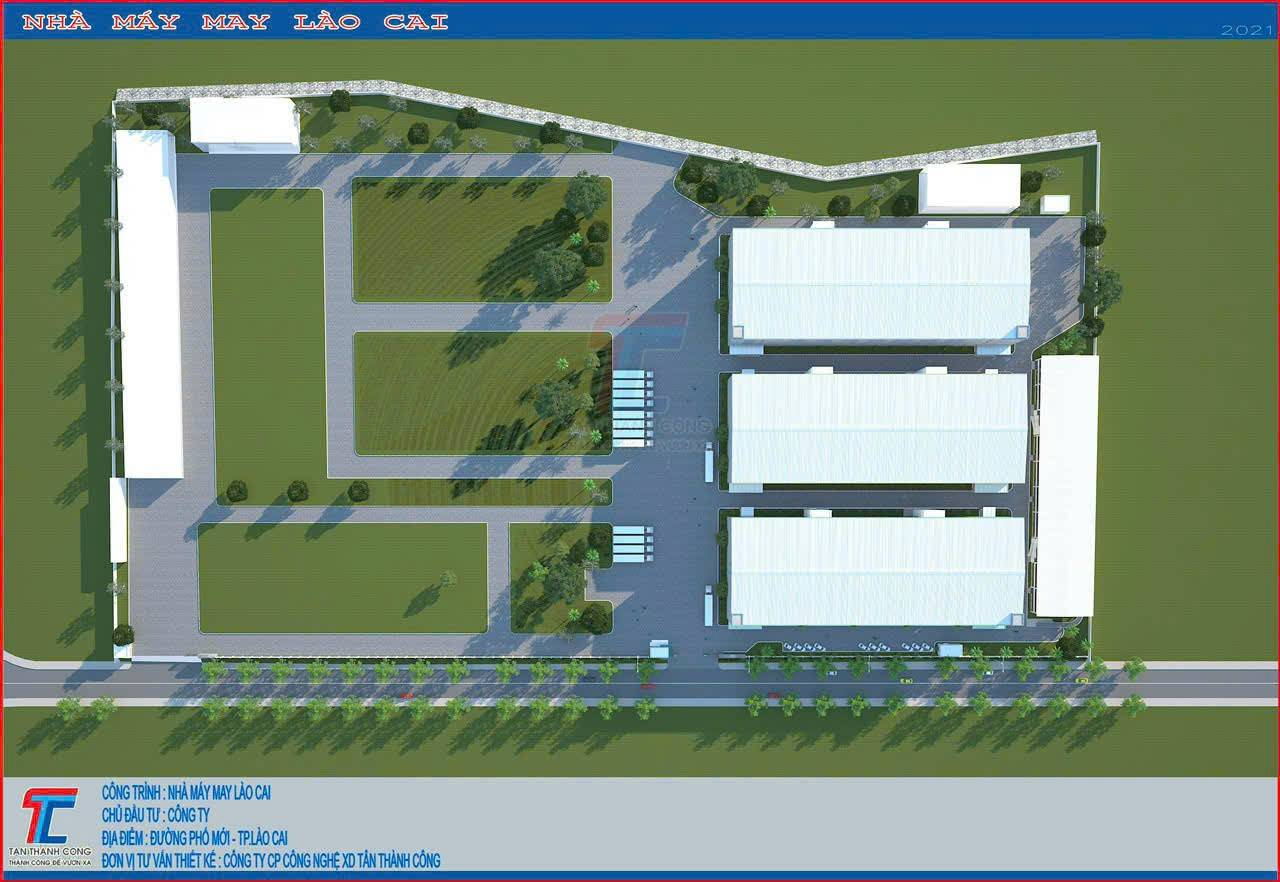
\includegraphics[width=42mm,height=32mm]{../../public/project-assets/laocai_3.jpg}};
  \end{scope}
  \draw[white,line width=1.2pt,rounded corners=2pt] (70,184) rectangle (101,216);
  \fill[TTCDeepNavy,opacity=.88] (70,184) rectangle (101,191);
  \node[anchor=west,text=white,font=\fontsize{4.6}{5.4}\selectfont\bfseries]
    at (72,187.5) {PLANNING PLAN};
  \draw[TTCBorder,rounded corners=4pt,line width=.7pt] (0,148) rectangle (104,220);

  % Thẻ dữ liệu dự án (phải)
  \fill[TTCDeepNavy,rounded corners=4pt] (108,148) rectangle (186,220);
  \node[anchor=north west,text=TTCCyan,font=\fontsize{6.8}{8}\selectfont\bfseries]
    at (114,214) {DESIGN CONSULTANCY \& CONSTRUCTION};
  \node[anchor=north west,text=white,font=\fontsize{11.5}{13}\selectfont\bfseries]
    at (114,204) {LAO CAI GARMENT FACTORY};
  \node[anchor=north west,text=white!75!gray,font=\fontsize{6}{7.2}\selectfont]
    at (114,192) {COMPLEX OF 3 BLOCKS OF 5-STOREY FACTORY};
  \draw[white!25!gray] (114,186) -- (180,186);
  \node[anchor=north west,text width=66mm,align=left,text=white,
        font=\fontsize{6.5}{8.5}\selectfont]
    at (114,181) {\textbf{Client:} Lao Cai Garment Company\\[1mm]
                  \textbf{Location:} New Street, Lao Cai City\\[1mm]
                  \textbf{Scale:} 3 5-storey workshop block • Import and export area\\[1mm]
                  \textbf{Tan Thanh Cong JSC:} Architectural design \& General Contractor};

  % Khung sơ đồ kỹ thuật
  \node[anchor=west,text=TTCBlue,font=\fontsize{8}{9.5}\selectfont\bfseries]
    at (0,141) {PRINCIPLE DIAGRAM • HIGH-RISE GARMENT FACTORY \& SOUND PRESSURE MICROCLIMATE};
  \fill[TTCLightBlue,rounded corners=4pt] (0,53) rectangle (186,134);
  \draw[TTCBorder,rounded corners=4pt,line width=.7pt] (0,53) rectangle (186,134);

  % Vùng phân tích kỹ thuật bên phải sơ đồ
  \fill[white,rounded corners=3pt] (130,58) rectangle (181,129);
  \draw[TTCBorder,rounded corners=3pt,line width=.6pt] (130,58) rectangle (181,129);
  \node[anchor=north west,text=TTCBlue,font=\fontsize{7.2}{8.5}\selectfont\bfseries]
    at (134,125) {3 TECHNICAL DECISIONS};

  \node[anchor=north west,text width=44mm,font=\fontsize{5.8}{7.2}\selectfont]
    at (134,117) {\textbf{01 • Load-bearing multi-storey floor}\\[.3mm]
    \color{TTCTextDark}Composite floor beams suppress resonant vibration from thousands of sewing machines.};

  \node[anchor=north west,text width=44mm,font=\fontsize{5.8}{7.2}\selectfont]
    at (134,94) {\textbf{02 • Negative pressure microclimate}\\[.3mm]
    \color{TTCTextDark}Cooling Pad \& convection exhaust fan, cotton dust purification and continuous fresh air supply.};

  \node[anchor=north west,text width=44mm,font=\fontsize{5.8}{7.2}\selectfont]
    at (134,71) {\textbf{03 • Cluster of 3 workshop blocks}\\[.3mm]
    \color{TTCTextDark}Planning the import and export flow of containers and elevators according to operating requirements.};

  % Bản vẽ mặt cắt nhà xưởng may nhiều tầng (Multi-storey Garment Factory Cross-section)
  % Khung kết cấu bao che
  \draw[TTCBlue,line width=1.4pt] (10,65) -- (10,123) -- (67,130) -- (124,123) -- (124,65);

  % Cột chịu lực giữa (mờ để không rối text)
  \draw[TTCBlue!40,line width=.8pt,dashed] (48,65) -- (48,127);
  \draw[TTCBlue!40,line width=.8pt,dashed] (86,65) -- (86,127);

  % Trục thang nâng hàng tải nặng (Freight Elevator Shaft) bên trái
  \fill[TTCDeepNavy!15] (10,65) rectangle (24,123);
  \draw[TTCBlue,line width=1.1pt] (24,65) -- (24,123);
  \node[rotate=90,align=center,text=TTCDeepNavy,font=\fontsize{5.2}{6.2}\selectfont\bfseries] at (17,94) {3--5 TON LIFT};

  % Các tầng sàn dầm thép liên hợp (Floor slabs)
  \draw[TTCBlue,line width=1.2pt] (24,78) -- (124,78);
  \draw[TTCBlue,line width=1.2pt] (24,91) -- (124,91);
  \draw[TTCBlue,line width=1.2pt] (24,104) -- (124,104);
  \draw[TTCBlue,line width=1.2pt] (24,117) -- (124,117);

  % Text nhãn từng tầng
  \node[anchor=west,text=TTCBlue,font=\fontsize{5.2}{6.2}\selectfont\bfseries] at (26,74) {1ST FLOOR: RAW MATERIAL WAREHOUSE \& EXPORT AND IMPORT OF FINISHED PRODUCTS};
  \node[anchor=west,text=TTCBlue,font=\fontsize{5.2}{6.2}\selectfont\bfseries] at (26,87) {2ND FLOOR: CUTTING WORKSHOP \& SEWING SAMPLE};
  \node[anchor=west,text=TTCBlue,font=\fontsize{5.2}{6.2}\selectfont\bfseries] at (26,100) {3RD FLOOR: EXPORT SEWING LINE 01};
  \node[anchor=west,text=TTCBlue,font=\fontsize{5.2}{6.2}\selectfont\bfseries] at (26,113) {4TH FLOOR: EXPORT SEWING LINE 02};
  \node[anchor=west,text=TTCBlue,font=\fontsize{5.2}{6.2}\selectfont\bfseries] at (26,122.5) {5TH FLOOR: FINISHING, COMFORTING \& PACKAGING};

  % Biểu tượng máy may trên các tầng 2, 3, 4
  \foreach \y in {78, 91, 104}{
    \foreach \x in {34, 58, 74, 98, 114}{
      \fill[white] (\x-3.5,\y+1.5) rectangle +(6.5,4);
      \draw[TTCBorder,line width=.4pt] (\x-3.5,\y+1.5) rectangle +(6.5,4);
      \draw[TTCRed,line width=.5pt] (\x-1.5,\y+2.5) -- (\x+1.5,\y+2.5);
    }
  }

  % Tuyến làm mát áp suất âm & Hút bụi vải (Cooling & Exhaust airflow)
  \foreach \y in {70, 82.5, 95.5, 108.5}{
    \draw[TTCCyan,line width=.8pt,dash pattern=on 3pt off 2pt] (26,\y) -- (122,\y);
    \draw[-{Latex[length=1.1mm]},TTCCyan,line width=.7pt] (62,\y) -- (70,\y);
    \draw[-{Latex[length=1.1mm]},TTCCyan,line width=.7pt] (98,\y) -- (106,\y);
  }

  % Móng & Sàn liên hợp đáy
  \fill[TTCDeepNavy] (9,58) rectangle (125,65);
  \node[anchor=center,text=white,font=\fontsize{5.4}{6.5}\selectfont\bfseries]
    at (67,61.5) {COMBINED FLOOR BEAMS UNDER DYNAMIC LOAD OF SEWING MACHINE};

  % 3 Thẻ ghi nhớ dưới
  \fill[white,rounded corners=3pt] (0,20) rectangle (58,52);
  \draw[TTCBorder,rounded corners=3pt,line width=.7pt] (0,20) rectangle (58,52);
  \node[anchor=north west,text=TTCRed,font=\fontsize{8}{9}\selectfont\bfseries]
    at (5,47) {01 • HIGH-RISE GARMENT FACTORY};
  \node[anchor=north west,text width=48mm,text=TTCTextDark,font=\fontsize{6.8}{8.4}\selectfont]
    at (5,38) {The complex of 3 blocks of 5 floors optimizes the density of land use and the arrangement of lines.};

  \fill[white,rounded corners=3pt] (64,20) rectangle (122,52);
  \draw[TTCBorder,rounded corners=3pt,line width=.7pt] (64,20) rectangle (122,52);
  \node[anchor=north west,text=TTCBlue,font=\fontsize{8}{9}\selectfont\bfseries]
    at (69,47) {02 • TEXTILE CLIMATE};
  \node[anchor=north west,text width=48mm,text=TTCTextDark,font=\fontsize{6.8}{8.4}\selectfont]
    at (69,38) {Negative pressure cooling, cotton dust filtration and fresh air supply meet export audit standards.};

  \fill[white,rounded corners=3pt] (128,20) rectangle (186,52);
  \draw[TTCBorder,rounded corners=3pt,line width=.7pt] (128,20) rectangle (186,52);
  \node[anchor=north west,text=TTCBlue,font=\fontsize{8}{9}\selectfont\bfseries]
    at (133,47) {03 • GENERAL CONTRACTOR D\&B};
  \node[anchor=north west,text width=48mm,text=TTCTextDark,font=\fontsize{6.8}{8.4}\selectfont]
    at (133,38) {Consulting on architectural design, composite structure and complete construction of the package.};

  \fill[TTCDeepNavy,rounded corners=3pt] (0,0) rectangle (186,14);
  \node[anchor=west,text=white,font=\fontsize{7.4}{9}\selectfont\bfseries]
    at (7,7) {CORE VALUES: HIGH-RISE FACTORY SOLUTIONS • STANDARD WORKING ENVIRONMENT FOR EXPORT};
\end{tikzpicture}
\end{minipage}
\newpage

% ============================================================
% PAGE 26: CASE STUDY 05 -- NHÀ MÁY NHỰA DHL
% ============================================================
\noindent\mbox{}\par\vspace{-\baselineskip}
\casepagebars{ENGINEERING SOLUTION • DHL PLASTICS GROUP}{Page 26}

\begin{minipage}[t][246mm]{\textwidth}
\secbrand{Project Profile 05: Manufacturing Plant DHL Plastic}{High-grade plastic packaging plant • PE/PP film extrusion • Thai Ha Industrial Park, Ha Nam}

\noindent
\begin{tikzpicture}[x=1mm,y=1mm]
  \path[use as bounding box] (0,0) rectangle (186,220);

  % Ảnh hoàn thiện làm hình chính; phối cảnh thiết kế làm hình đối chiếu
  \begin{scope}
    \clip[rounded corners=4pt] (0,148) rectangle (104,220);
    \node[inner sep=0pt] at (52,184)
      {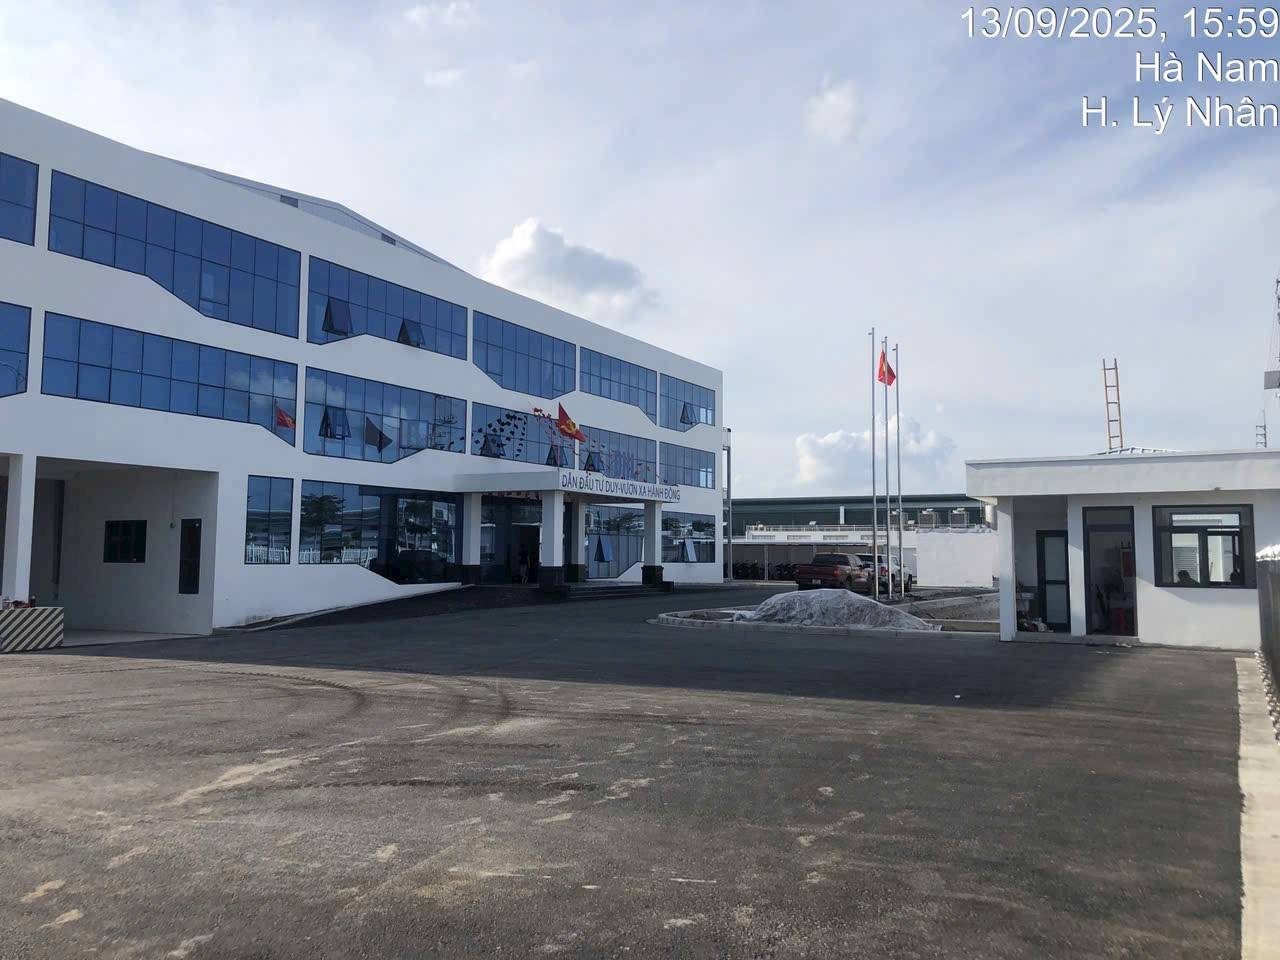
\includegraphics[width=104mm]{../../public/project-assets/dhl_2.jpg}};
    \fill[TTCDeepNavy,opacity=.92] (0,148) rectangle (104,158);
    \node[anchor=west,text=white,font=\fontsize{6.8}{8}\selectfont\bfseries]
      at (4,153) {ACTUAL PHOTOS COMPLETED • THAI HA INDUSTRIAL ZONE, HA NAM};
  \end{scope}
  \begin{scope}
    \clip[rounded corners=2pt] (71,184) rectangle (101,216);
    \node[inner sep=0pt] at (86,200)
      {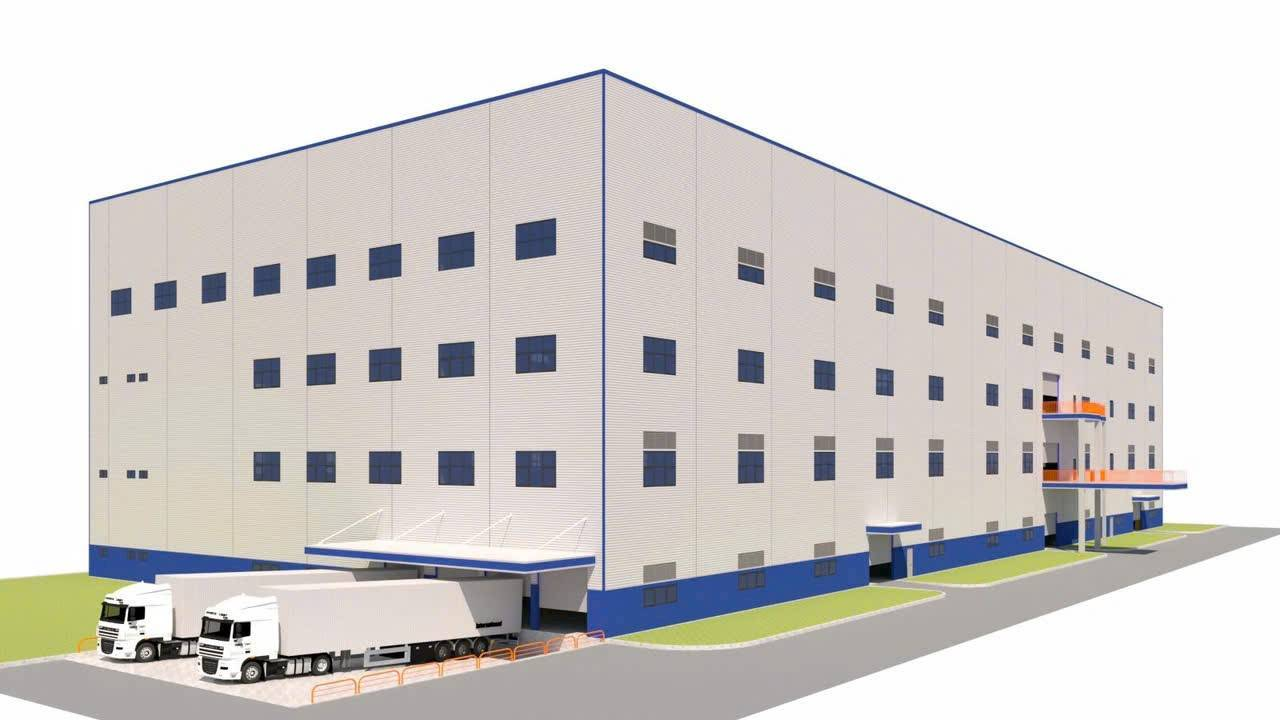
\includegraphics[width=42mm,height=32mm]{../../public/project-assets/dhl_4.jpg}};
  \end{scope}
  \draw[white,line width=1.2pt,rounded corners=2pt] (71,184) rectangle (101,216);
  \fill[TTCDeepNavy,opacity=.88] (71,184) rectangle (101,191);
  \node[anchor=west,text=white,font=\fontsize{4.6}{5.4}\selectfont\bfseries]
    at (73,187.5) {DESIGN PERSPECTIVE};
  \draw[TTCBorder,rounded corners=4pt,line width=.7pt] (0,148) rectangle (104,220);

  % Thẻ dữ liệu dự án (phải)
  \fill[TTCDeepNavy,rounded corners=4pt] (108,148) rectangle (186,220);
  \node[anchor=north west,text=TTCCyan,font=\fontsize{6.8}{8}\selectfont\bfseries]
    at (114,214) {GENERAL CONTRACTOR};
  \node[anchor=north west,text=white,font=\fontsize{11.5}{13}\selectfont\bfseries]
    at (114,204) {DHL PLASTIC FACTORY};
  \node[anchor=north west,text=white!75!gray,font=\fontsize{6}{7.2}\selectfont]
    at (114,192) {FACTORY COMPLEX \& OFFICE BLOCK};
  \draw[white!25!gray] (114,186) -- (180,186);
  \node[anchor=north west,text width=66mm,align=left,text=white,
        font=\fontsize{6.5}{8.5}\selectfont]
    at (114,181) {\textbf{Client:} DHL Plastic Group Joint Stock Company\\[1mm]
                  \textbf{Location:} Lot CN02, Thai Ha Industrial Park, Ha Nam\\[1mm]
                  \textbf{Scale:} PE/PP Film Workshop Complex \& 3-storey office\\[1mm]
                  \textbf{Tan Thanh Cong JSC:} PEB General Contractor \& Electromechanical MEP};

  % Khung sơ đồ kỹ thuật
  \node[anchor=west,text=TTCBlue,font=\fontsize{8}{9.5}\selectfont\bfseries]
    at (0,141) {PRINCIPLE DIAGRAM • PLASTIC FILM BLOWING EXTRUSION LINE \& MEP BACKEND SYSTEM};
  \fill[TTCLightBlue,rounded corners=4pt] (0,53) rectangle (186,134);
  \draw[TTCBorder,rounded corners=4pt,line width=.7pt] (0,53) rectangle (186,134);

  % Vùng phân tích kỹ thuật bên phải sơ đồ
  \fill[white,rounded corners=3pt] (130,58) rectangle (181,129);
  \draw[TTCBorder,rounded corners=3pt,line width=.6pt] (130,58) rectangle (181,129);
  \node[anchor=north west,text=TTCBlue,font=\fontsize{7.2}{8.5}\selectfont\bfseries]
    at (134,125) {3 TECHNICAL DECISIONS};

  \node[anchor=north west,text width=44mm,font=\fontsize{5.8}{7.2}\selectfont]
    at (134,117) {\textbf{01 • Crossing the cascading span}\\[.3mm]
    \color{TTCTextDark}pre-engineered steel building large aperture frame integrates a cascade chamber for the extrusion tower.};

  \node[anchor=north west,text width=44mm,font=\fontsize{5.8}{7.2}\selectfont]
    at (134,94) {\textbf{02 • Extruded chiller infrastructure}\\[.3mm]
    \color{TTCTextDark}The circulating cold water system keeps the temperature stable and the thin film stable.};

  \node[anchor=north west,text width=44mm,font=\fontsize{5.8}{7.2}\selectfont]
    at (134,71) {\textbf{03 • Hardener floor under load}\\[.3mm]
    \color{TTCTextDark}The grinding concrete surface is hardened, dustproof and designed according to the forklift load.};

  % Bản vẽ sơ đồ phân xưởng đùn màng & in bao bì
  % Khung kết cấu nhà xưởng có tháp cao thông tầng
  \draw[TTCBlue,line width=1.4pt] (10,65) -- (10,128) -- (48,128) -- (48,118) -- (124,118) -- (124,65);
  \draw[TTCBlue!40,line width=.8pt,dashed] (86,65) -- (86,118);

  % Tháp đùn thổi màng (Blown Film Tower)
  \fill[white] (15,70) rectangle (43,124);
  \draw[TTCBlue,line width=.9pt] (15,70) rectangle (43,124);
  \draw[TTCRed,line width=1pt] (29,74) -- (29,114);
  \draw[TTCCyan,line width=.8pt] (24,74) .. controls (19,94) and (21,110) .. (29,114);
  \draw[TTCCyan,line width=.8pt] (34,74) .. controls (39,94) and (37,110) .. (29,114);
  \fill[TTCBlue] (26,114) rectangle (32,118);
  \node[align=center,text=TTCBlue,font=\fontsize{5.2}{6.2}\selectfont\bfseries]
    at (29,84) {BLOWING EXTRUSION TOWER\\MULTILAYER MEMBRANE\\CASCADE COMPARTMENT};

  % Cụm máy in ấn ống đồng & cuộn màng
  \fill[white] (52,70) rectangle (82,94);
  \draw[TTCBorder,line width=.7pt] (52,70) rectangle (82,94);
  \fill[TTCLightBlue] (55,73) rectangle (79,83);
  \draw[TTCBlue,line width=.6pt] (55,73) rectangle (79,83);
  \node[align=center,text=TTCBlue,font=\fontsize{5.2}{6.2}\selectfont\bfseries]
    at (67,88) {GRAVURE PRINTER \&\\AUTOMATIC FILM REEL};
  \node[align=center,text=TTCTextDark,font=\fontsize{4.8}{5.8}\selectfont]
    at (67,78) {SPEED MULTI-COLOR PRINTING HEIGHT};

  % Cụm lưu trữ nguyên liệu & kho thành phẩm
  \fill[white] (88,70) rectangle (120,94);
  \draw[TTCBorder,line width=.7pt] (88,70) rectangle (120,94);
  \node[align=center,text=TTCBlue,font=\fontsize{5.2}{6.2}\selectfont\bfseries]
    at (104,88) {FINISHED GOODS WAREHOUSE \&\\PROTOPLASTIC BEADS};
  \foreach \x in {93, 104, 115}{
    \fill[TTCDeepNavy!20] (\x-3,73) rectangle +(6,8);
    \draw[TTCDeepNavy,line width=.4pt] (\x-3,73) rectangle +(6,8);
  }

  % Tuyến đường ống Chiller tuần hoàn & Khí nén
  \draw[TTCCyan,line width=1.1pt,dashed] (12,104) -- (122,104);
  \node[anchor=west,text=TTCCyan,font=\fontsize{5.8}{7}\selectfont\bfseries]
    at (50,107.5) {AXLE COOLING CHILLER PIPE \& MEDIUM COMPRESSED AIR DEDICATION};
  \draw[-{Latex[length=1.2mm]},TTCCyan,line width=.7pt] (29,104) -- (29,95);
  \draw[-{Latex[length=1.2mm]},TTCCyan,line width=.7pt] (67,104) -- (67,96);

  % Móng & Sàn bê tông Hardener
  \fill[TTCDeepNavy] (9,58) rectangle (125,65);
  \node[anchor=center,text=white,font=\fontsize{5.4}{6.5}\selectfont\bfseries]
    at (67,61.5) {HARDENED POLISHED CONCRETE FLOOR HARDENER AGAINST DUST};

  % 3 Thẻ ghi nhớ dưới
  \fill[white,rounded corners=3pt] (0,20) rectangle (58,52);
  \draw[TTCBorder,rounded corners=3pt,line width=.7pt] (0,20) rectangle (58,52);
  \node[anchor=north west,text=TTCRed,font=\fontsize{8}{9}\selectfont\bfseries]
    at (5,47) {01 • WORKSHOP COMPLEX \& VP};
  \node[anchor=north west,text width=48mm,text=TTCTextDark,font=\fontsize{6.8}{8.4}\selectfont]
    at (5,38) {Modern 3-storey glass office block combined with large-scale film blowing extrusion workshop.};

  \fill[white,rounded corners=3pt] (64,20) rectangle (122,52);
  \draw[TTCBorder,rounded corners=3pt,line width=.7pt] (64,20) rectangle (122,52);
  \node[anchor=north west,text=TTCBlue,font=\fontsize{8}{9}\selectfont\bfseries]
    at (69,47) {02 • HIGH POWER MEP};
  \node[anchor=north west,text width=48mm,text=TTCTextDark,font=\fontsize{6.8}{8.4}\selectfont]
    at (69,38) {Integrated substation, extruder cooling chiller tower and central compressed air synchronously.};

  \fill[white,rounded corners=3pt] (128,20) rectangle (186,52);
  \draw[TTCBorder,rounded corners=3pt,line width=.7pt] (128,20) rectangle (186,52);
  \node[anchor=north west,text=TTCBlue,font=\fontsize{8}{9}\selectfont\bfseries]
    at (133,47) {03 • ACTUAL HANDOVER};
  \node[anchor=north west,text width=48mm,text=TTCTextDark,font=\fontsize{6.8}{8.4}\selectfont]
    at (133,38) {Accurate construction, inspection and acceptance of safety fire prevention and fighting and put into commercial operation by 2025.};

  \fill[TTCDeepNavy,rounded corners=3pt] (0,0) rectangle (186,14);
  \node[anchor=west,text=white,font=\fontsize{7.4}{9}\selectfont\bfseries]
    at (7,7) {CORE VALUES: HIGH-GRADE PLASTIC PACKAGING PRODUCTION INFRASTRUCTURE • ACTUAL HANDOVER QUALITY};
\end{tikzpicture}
\end{minipage}
\newpage

% ============================================================
% PAGE 27: CASE STUDY 06 -- NHÀ MÁY NHÔM QUANG THỊNH
% ============================================================
\noindent\mbox{}\par\vspace{-\baselineskip}
\casepagebars{ENGINEERING SOLUTION • QUANG THINH ALUMINIUM}{Page 27}

\begin{minipage}[t][246mm]{\textwidth}
\secbrand{Project Profile 06: Manufacturing Plant Quang Thinh Aluminum}{High-grade aluminum profiles plant • Heavy extrusion lines • Thuan Thanh, Bac Ninh}

\noindent
\begin{tikzpicture}[x=1mm,y=1mm]
  \path[use as bounding box] (0,0) rectangle (186,220);

  % Ảnh phối cảnh dự án (trái)
  \begin{scope}
    \clip[rounded corners=4pt] (0,148) rectangle (104,220);
    \node[inner sep=0pt] at (52,198)
      {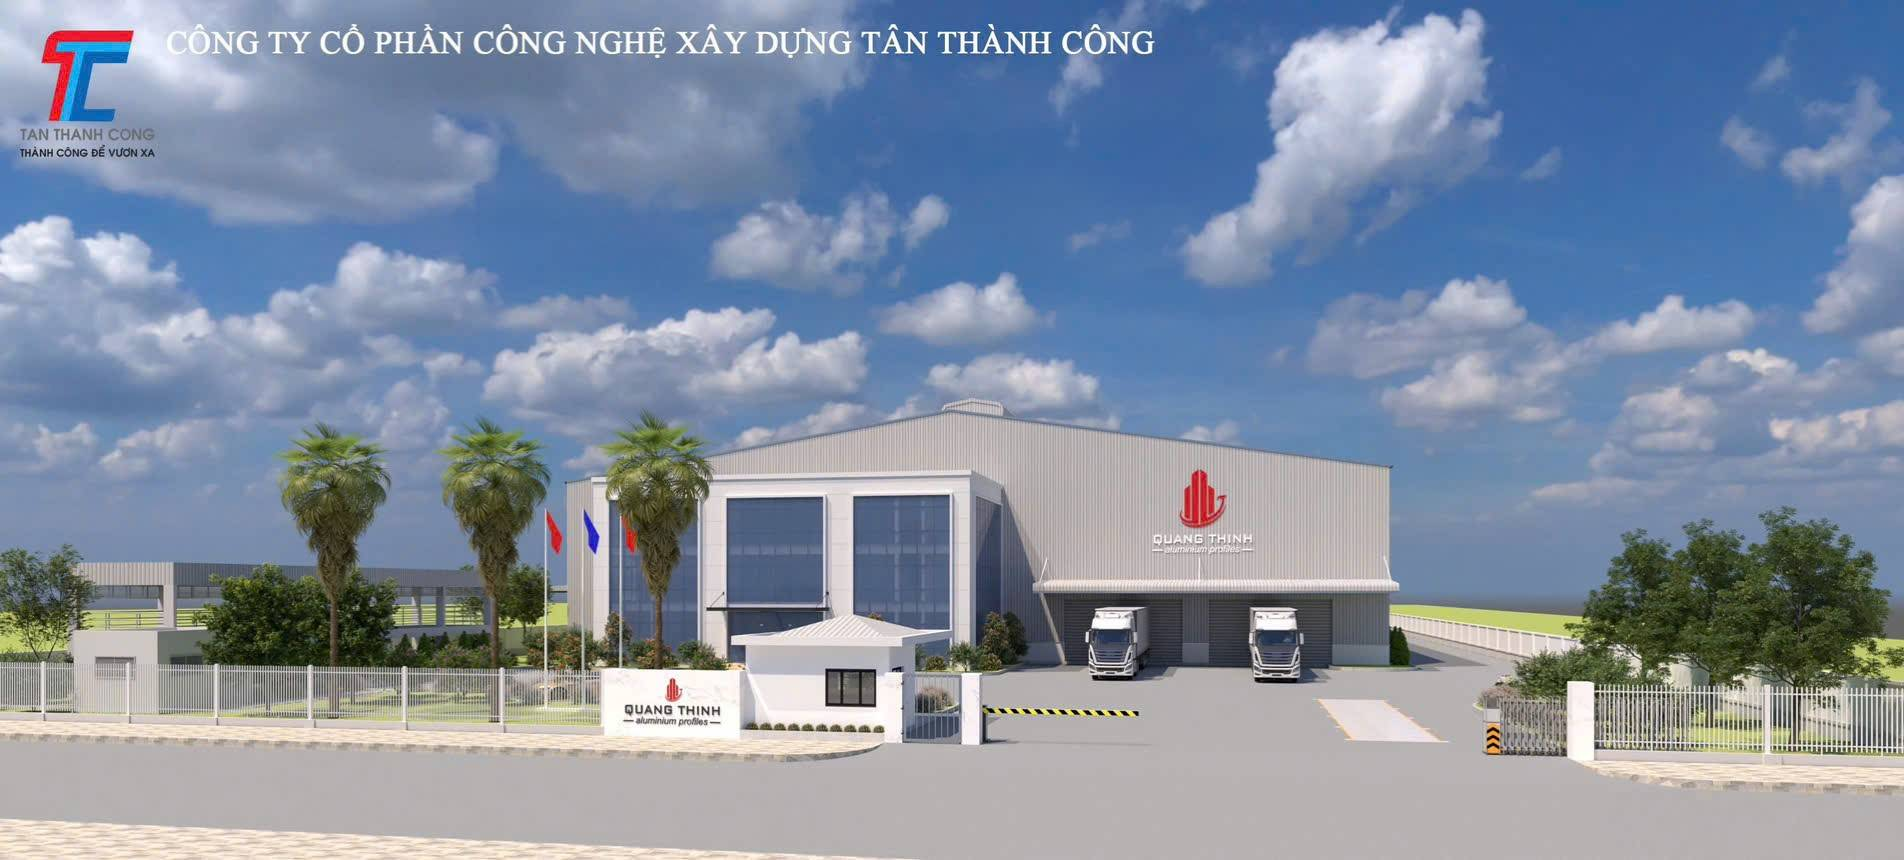
\includegraphics[width=185mm]{../../public/project-assets/quangthinh_1.jpg}};
    \fill[TTCDeepNavy,opacity=.92] (0,148) rectangle (104,158);
    \node[anchor=west,text=white,font=\fontsize{6.8}{8}\selectfont\bfseries]
      at (4,153) {PROJECT PERSPECTIVE • THUAN THANH, BAC NINH};
  \end{scope}
  % Ảnh hiện trường bổ sung giúp phân biệt phối cảnh với tiến độ thi công thực tế
  \begin{scope}
    \clip[rounded corners=2pt] (70,181) rectangle (101,216);
    \node[inner sep=0pt] at (85.5,198.5)
      {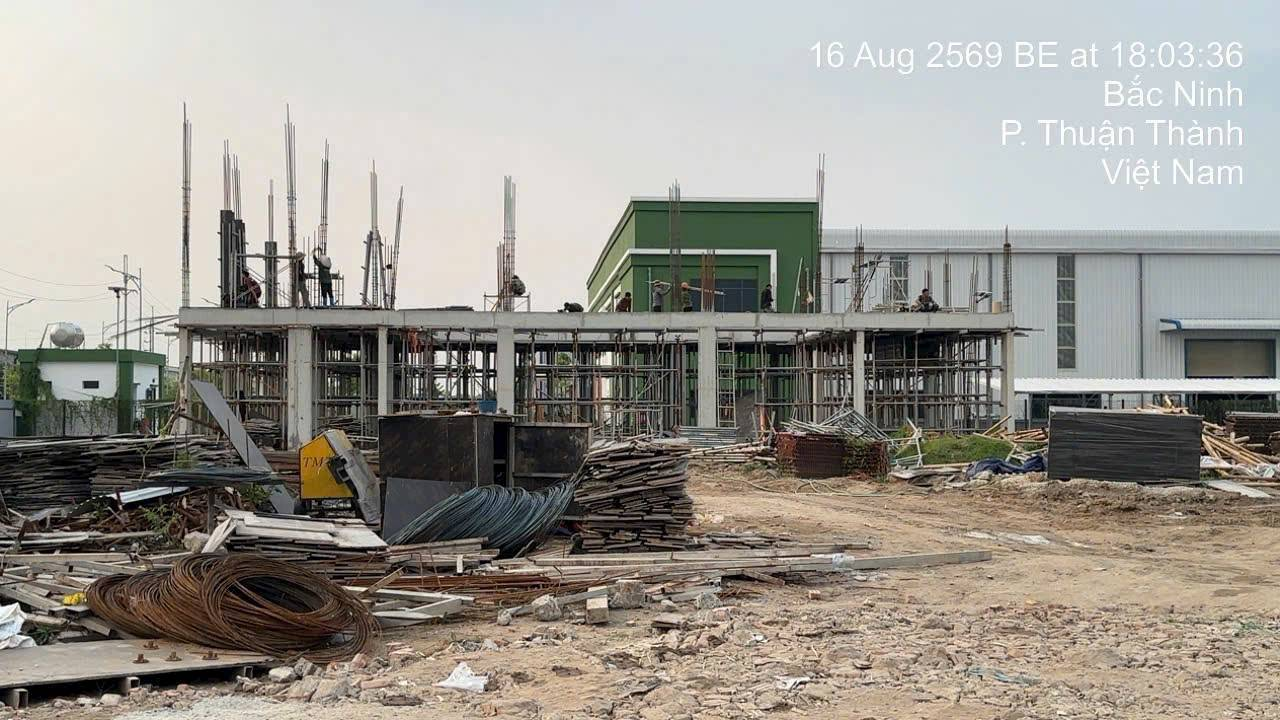
\includegraphics[width=46mm,height=35mm]{../../public/project-assets/quangthinh_3.jpg}};
  \end{scope}
  \draw[white,line width=1.2pt,rounded corners=2pt] (70,181) rectangle (101,216);
  \fill[TTCDeepNavy,opacity=.88] (70,181) rectangle (101,188);
  \node[anchor=west,text=white,font=\fontsize{4.6}{5.4}\selectfont\bfseries]
    at (72,184.5) {ACTUAL CONSTRUCTION PHOTOS};
  \draw[TTCBorder,rounded corners=4pt,line width=.7pt] (0,148) rectangle (104,220);

  % Thẻ dữ liệu dự án (phải)
  \fill[TTCDeepNavy,rounded corners=4pt] (108,148) rectangle (186,220);
  \node[anchor=north west,text=TTCCyan,font=\fontsize{6.8}{8}\selectfont\bfseries]
    at (114,214) {GENERAL CONTRACTOR};
  \node[anchor=north west,text=white,font=\fontsize{11.2}{13}\selectfont\bfseries]
    at (114,204) {QUANG THINH ALUMINUM FACTORY};
  \node[anchor=north west,text=white!75!gray,font=\fontsize{6}{7.2}\selectfont]
    at (114,192) {EXTRUSION FACTORY COMPLEX \& POWDER COATING};
  \draw[white!25!gray] (114,186) -- (180,186);
  \node[anchor=north west,text width=66mm,align=left,text=white,
        font=\fontsize{6.5}{8.5}\selectfont]
    at (114,181) {\textbf{Client:} Quang Thinh Aluminum Joint Stock Company\\[1mm]
                  \textbf{Location:} Thuan Thanh, Bac Ninh\\[1mm]
                  \textbf{Scale:} Extrusion workshop complex \& Executive office building\\[1mm]
                  \textbf{Tan Thanh Cong JSC:} PEB General Contractor \& Electromechanical MEP};

  % Khung sơ đồ kỹ thuật
  \node[anchor=west,text=TTCBlue,font=\fontsize{8}{9.5}\selectfont\bfseries]
    at (0,141) {PRINCIPLE DIAGRAM • ALUMINUM PROFILE EXTRUSION LINE \& SURFACE TREATMENT};
  \fill[TTCLightBlue,rounded corners=4pt] (0,53) rectangle (186,134);
  \draw[TTCBorder,rounded corners=4pt,line width=.7pt] (0,53) rectangle (186,134);

  % Vùng phân tích kỹ thuật bên phải sơ đồ
  \fill[white,rounded corners=3pt] (130,58) rectangle (181,129);
  \draw[TTCBorder,rounded corners=3pt,line width=.6pt] (130,58) rectangle (181,129);
  \node[anchor=north west,text=TTCBlue,font=\fontsize{7.2}{8.5}\selectfont\bfseries]
    at (134,125) {3 TECHNICAL DECISIONS};

  \node[anchor=north west,text width=44mm,font=\fontsize{5.8}{7.2}\selectfont]
    at (134,117) {\textbf{01 • Heavy duty extruder foundation}\\[.3mm]
    \color{TTCTextDark}The large block reinforced concrete foundation is designed according to the dynamic load of the hydraulic press.};

  \node[anchor=north west,text width=44mm,font=\fontsize{5.8}{7.2}\selectfont]
    at (134,94) {\textbf{02 • Powder coating line}\\[.3mm]
    \color{TTCTextDark}Closed spray booth, high temperature oven and Anode plating wastewater treatment station.};

  \node[anchor=north west,text width=44mm,font=\fontsize{5.8}{7.2}\selectfont]
    at (134,71) {\textbf{03 • Wear-Resistant Hardener Flooring}\\[.3mm]
    \color{TTCTextDark}The grinding concrete surface is hardened, dustproof and designed according to the load of the workpiece forklift.};

  % Bản vẽ sơ đồ phân xưởng đùn ép nhôm định hình
  % Khung kết cấu nhà xưởng PEB
  \draw[TTCBlue,line width=1.4pt] (10,65) -- (10,126) -- (67,126) -- (124,126) -- (124,65);
  \draw[TTCBlue!40,line width=.8pt,dashed] (48,65) -- (48,126);
  \draw[TTCBlue!40,line width=.8pt,dashed] (86,65) -- (86,126);

  % Dầm cầu trục phục vụ dây chuyền
  \draw[TTCBlue,line width=1pt] (10,113) -- (124,113);
  \fill[TTCBlue] (26,111) rectangle (36,115);
  \fill[TTCBlue] (70,111) rectangle (80,115);
  \node[anchor=west,text=TTCBlue,font=\fontsize{5.2}{6.2}\selectfont\bfseries]
    at (14,118) {CRANE GIRDER FOR ALUMINUM WORKPIECE LIFTING \& CHANGE EXTRUSION MOLD};

  % Zone 1: Lò nung phôi nhôm & Máy đùn ép thủy lực
  \fill[white] (13,70) rectangle (46,96);
  \draw[TTCBorder,line width=.7pt] (13,70) rectangle (46,96);
  \fill[TTCRed!15] (16,73) rectangle (43,83);
  \draw[TTCRed,line width=.6pt] (16,73) rectangle (43,83);
  \node[align=center,text=TTCBlue,font=\fontsize{5.1}{6.1}\selectfont\bfseries]
    at (29.5,90) {ALUMINUM BLAST FURNACE \&\\HYDRAULIC EXTRUDER};
  \node[align=center,text=TTCRed,font=\fontsize{4.8}{5.8}\selectfont\bfseries]
    at (29.5,78) {EXTRUSION BY LINE};

  % Zone 2: Dàn làm nguội & Bàn kéo dài thanh nhôm
  \fill[white] (49,70) rectangle (84,96);
  \draw[TTCBorder,line width=.7pt] (49,70) rectangle (84,96);
  \fill[TTCLightBlue] (52,73) rectangle (81,83);
  \draw[TTCBlue,line width=.6pt] (52,73) rectangle (81,83);
  \node[align=center,text=TTCBlue,font=\fontsize{5.1}{6.1}\selectfont\bfseries]
    at (66.5,90) {COOLING STRETCHING TABLE \&\\HOMOGENIZING FURNACE};
  \node[align=center,text=TTCTextDark,font=\fontsize{4.8}{5.8}\selectfont]
    at (66.5,78) {CONFIGURE LONG PROFILE};

  % Zone 3: Dây chuyền sơn tĩnh điện & Đóng gói
  \fill[white] (87,70) rectangle (121,96);
  \draw[TTCBorder,line width=.7pt] (87,70) rectangle (121,96);
  \fill[TTCDeepNavy!15] (90,73) rectangle (118,83);
  \draw[TTCDeepNavy,line width=.6pt] (90,73) rectangle (118,83);
  \node[align=center,text=TTCBlue,font=\fontsize{5.1}{6.1}\selectfont\bfseries]
    at (104,90) {POWDER COATING LINE\\\& FINISHED PRODUCT PACKAGING};
  \node[align=center,text=TTCTextDark,font=\fontsize{4.8}{5.8}\selectfont]
    at (104,78) {ANODE PLATING • HANGING PAINT};

  % Mũi tên chuyển bước dây chuyền
  \draw[-{Latex[length=1.4mm]},TTCBlue,line width=1pt] (46,83) -- (49,83);
  \draw[-{Latex[length=1.4mm]},TTCBlue,line width=1pt] (84,83) -- (87,83);

  % Tuyến đường ống Chiller giải nhiệt khuôn đùn ép & Khí nén
  \draw[TTCCyan,line width=1.1pt,dashed] (12,103) -- (122,103);
  \node[anchor=west,text=TTCCyan,font=\fontsize{5.8}{7}\selectfont\bfseries]
    at (36,106.5) {EXTRUSION MOLD COOLING WATER SYSTEM \& MEDIUM COMPRESSED AIR DEDICATION};
  \draw[-{Latex[length=1.2mm]},TTCCyan,line width=.7pt] (29.5,103) -- (29.5,97);
  \draw[-{Latex[length=1.2mm]},TTCCyan,line width=.7pt] (66.5,103) -- (66.5,97);

  % Móng & Sàn bê tông Hardener
  \fill[TTCDeepNavy] (9,58) rectangle (125,65);
  \node[anchor=center,text=white,font=\fontsize{5.4}{6.5}\selectfont\bfseries]
    at (67,61.5) {FLOOR CONCRETE GRINDING HARDENER HARDENER ABRASION RESISTANT};

  % 3 Thẻ ghi nhớ dưới
  \fill[white,rounded corners=3pt] (0,20) rectangle (58,52);
  \draw[TTCBorder,rounded corners=3pt,line width=.7pt] (0,20) rectangle (58,52);
  \node[anchor=north west,text=TTCRed,font=\fontsize{8}{9}\selectfont\bfseries]
    at (5,47) {01 • EXTRUSION OF HEAVY LOADS};
  \node[anchor=north west,text width=48mm,text=TTCTextDark,font=\fontsize{6.8}{8.4}\selectfont]
    at (5,38) {Large span workshop frame integrates hydraulic press foundation and double girder crane.};

  \fill[white,rounded corners=3pt] (64,20) rectangle (122,52);
  \draw[TTCBorder,rounded corners=3pt,line width=.7pt] (64,20) rectangle (122,52);
  \node[anchor=north west,text=TTCBlue,font=\fontsize{8}{9}\selectfont\bfseries]
    at (69,47) {02 • SURFACE TREATMENT \& MEP};
  \node[anchor=north west,text width=48mm,text=TTCTextDark,font=\fontsize{6.8}{8.4}\selectfont]
    at (69,38) {Automatic powder coating system, plating wastewater treatment station and central compressed air.};

  \fill[white,rounded corners=3pt] (128,20) rectangle (186,52);
  \draw[TTCBorder,rounded corners=3pt,line width=.7pt] (128,20) rectangle (186,52);
  \node[anchor=north west,text=TTCBlue,font=\fontsize{8}{9}\selectfont\bfseries]
    at (133,47) {03 • LUMP-SUM GENERAL CONTRACTOR};
  \node[anchor=north west,text width=48mm,text=TTCTextDark,font=\fontsize{6.8}{8.4}\selectfont]
    at (133,38) {Synchronous construction management from PEB structure, architectural completion to MEP operation.};

  \fill[TTCDeepNavy,rounded corners=3pt] (0,0) rectangle (186,14);
  \node[anchor=west,text=white,font=\fontsize{7.4}{9}\selectfont\bfseries]
    at (7,7) {CORE VALUES: HIGH-TECH ALUMINUM PROFILE PRODUCTION INFRASTRUCTURE • SYNCHRONOUS GENERAL CONTRACTOR SOLUTION};
\end{tikzpicture}
\end{minipage}
\newpage

% ============================================================
% PAGE 28: CHUỖI CUNG ỨNG KIỂM SOÁT
% ============================================================
\noindent\mbox{}\par\vspace{-\baselineskip}
\casepagebars{SUPPLY CHAIN • MATERIAL CONTROL}{Page 28}

\begin{minipage}[t][246mm]{\textwidth}
\secbrand{Lot-Controlled Supply Chain}{Approved sources • Material submittal • CO/CQ/MTC • Lot traceability}

\noindent
\begin{tikzpicture}[x=1mm,y=1mm]
  \path[use as bounding box] (0,0) rectangle (186,220);

  \node[anchor=west,text=TTCBlue,font=\fontsize{15}{17}\selectfont\bfseries]
    at (0,211) {MATERIALS ARE INSTALLED ONLY AFTER APPROVAL};
  \node[anchor=west,text=TTCTextMuted,font=\fontsize{7.2}{8.8}\selectfont]
    at (0,201) {A unified approval flow helps lock out quality, origin, and replaceability prior to purchase.};

  % Cột quy trình 4 cổng kiểm soát
  \fill[TTCDeepNavy,rounded corners=4pt] (0,79) rectangle (62,192);
  \node[anchor=west,text=TTCCyan,font=\fontsize{7}{8.3}\selectfont\bfseries]
    at (7,184) {4 CONTROL GATES};
  \draw[white!18!gray] (7,178) -- (55,178);

  \foreach \y/\n/\title/\desc in {
    158/01/SOURCE APPROVAL/Manufacturer • sample • technical data,
    134/02/COMPANY/CO--CQ • MTC • catalog • warranty,
    110/03/INPUT TEST/Lot label • size • condition • test,
    88/04/TRACEABILITY OF INSTALLATION/Lot of materials associated with the area and inspection and acceptance minutes}
  {
    \fill[white,rounded corners=2pt] (7,{\y-8}) rectangle (55,{\y+8});
    \fill[TTCRed] (7,{\y-8}) rectangle (16,{\y+8});
    \node[text=white,font=\fontsize{6.2}{7}\selectfont\bfseries] at (11.5,\y) {\n};
    \node[anchor=north west,text width=34mm,text=TTCBlue,
          font=\fontsize{6.7}{7.8}\selectfont\bfseries] at (19,{\y+5}) {\title};
    \node[anchor=north west,text width=34mm,text=TTCTextMuted,
          font=\fontsize{5.6}{6.7}\selectfont] at (19,{\y-1}) {\desc};
  }

  % Ma trận nhóm vật tư
  \fill[white,rounded corners=4pt] (67,79) rectangle (186,192);
  \draw[TTCBorder,rounded corners=4pt,line width=.7pt] (67,79) rectangle (186,192);
  \node[anchor=west,text=TTCBlue,font=\fontsize{8}{9.4}\selectfont\bfseries]
    at (74,184) {GROUP OF REFERENCE MATERIALS/ BRANDS};
  \node[anchor=west,text=TTCTextMuted,font=\fontsize{5.8}{7}\selectfont]
    at (74,176) {The final selection is in accordance with the material approval documents of each project.};

  \foreach \y/\n/\name/\brands/\control in {
    157/01/STEEL \& COVER/POSCO • Hoa Phat • BlueScope/MTC • steel grade • plating,
    134/02/SON \& CHEMICALS/Jotun • KCC • Sika/batch • DFT • fire prevention and fighting certification,
    111/03/ELECTRICITY \& MEP/Schneider • ABB • LS Vina/Catalogue • test • origin,
    88/04/HVAC \& Fire/Daikin • Grundfos • Tyco/Submittal • UL--FM upon request}
  {
    \fill[TTCLightBlue,rounded corners=2pt] (73,{\y-9}) rectangle (180,{\y+9});
    \node[anchor=west,text=TTCRed,font=\fontsize{6.4}{7.5}\selectfont\bfseries]
      at (78,{\y+4}) {\n};
    \node[anchor=west,text=TTCBlue,font=\fontsize{7}{8.2}\selectfont\bfseries]
      at (91,{\y+4}) {\name};
    \node[anchor=west,text=TTCTextDark,font=\fontsize{6.2}{7.3}\selectfont]
      at (91,{\y-2}) {\brands};
    \node[anchor=east,text=TTCTextMuted,font=\fontsize{5.6}{6.7}\selectfont]
      at (176,{\y-7}) {Control: \control};
  }

  % Ba lớp bảo chứng
  \node[anchor=west,text=TTCBlue,font=\fontsize{8}{9.4}\selectfont\bfseries]
    at (0,68) {THREE LAYERS OF PROTECTION BEFORE INSTALLATION};
  \foreach \xa/\xb/\n/\title/\desc in {
    0/58/01/CORRECT SOURCE/Approval documents matching manufacturer and origin,
    64/122/02/in ACCORDANCE WITH QUALITY/Specimen matching specifications and project standards,
    128/186/03/CORRECT LOCATION/Each lot associated with the minutes and the area of use}
  {
    \fill[white,rounded corners=3pt] (\xa,25) rectangle (\xb,60);
    \draw[TTCBorder,rounded corners=3pt] (\xa,25) rectangle (\xb,60);
    \node[anchor=west,text=TTCRed,font=\fontsize{7}{8}\selectfont\bfseries]
      at ({\xa+6},52) {\n};
    \node[anchor=west,text=TTCBlue,font=\fontsize{7.4}{8.7}\selectfont\bfseries]
      at ({\xa+17},52) {\title};
    \node[anchor=north west,text width=46mm,text=TTCTextMuted,
          font=\fontsize{6.2}{7.5}\selectfont] at ({\xa+6},43) {\desc};
  }

  \fill[TTCDeepNavy,rounded corners=3pt] (0,0) rectangle (186,16);
  \node[anchor=west,text=TTCCyan,font=\fontsize{6.3}{7.5}\selectfont\bfseries]
    at (7,8) {MATERIAL ASSURANCE};
  \node[anchor=east,text=white,font=\fontsize{7.2}{8.5}\selectfont\bfseries]
    at (179,8) {APPROVED SOURCE → VERIFIED LOT → TRACEABLE INSTALLATION};
\end{tikzpicture}
\end{minipage}
\newpage

% ============================================================
% PAGE 29: HỆ SINH THÁI CÔNG TRÌNH THEO NGÀNH
% ============================================================
\noindent\mbox{}\par\vspace{-\baselineskip}
\casepagebars{PROJECT ECOSYSTEM • SIX SECTORS}{Page 29}

\begin{minipage}[t][246mm]{\textwidth}
\secbrand{Six Facility Types — One Integrated Capability}{Representative sectors • Different operating demands • One coordinated EPC workflow}

\noindent
\begin{tikzpicture}[x=1mm,y=1mm]
  \path[use as bounding box] (0,0) rectangle (186,220);
  \node[anchor=west,text=TTCBlue,font=\fontsize{15}{17}\selectfont\bfseries]
    at (0,211) {DESIGN STARTS WITH HOW THE PLANT OPERATES};
  \node[anchor=west,text=TTCTextMuted,font=\fontsize{7.2}{8.8}\selectfont]
    at (0,201) {Each industry group has a core risk; the structural solution, MEP and construction sequence must answer that risk correctly.};

  % Hàng 1
  \begin{scope}
    \clip[rounded corners=3pt] (0,132) rectangle (59,190);
    \node[inner sep=0pt] at (29.5,165) {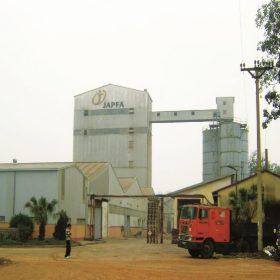
\includegraphics[width=60mm]{../../public/project-assets/japfa.jpg}};
    \fill[TTCDeepNavy,opacity=.9] (0,132) rectangle (59,151);
  \end{scope}
  \draw[TTCBorder,rounded corners=3pt] (0,132) rectangle (59,190);
  \node[anchor=west,text=white,font=\fontsize{7.5}{8.8}\selectfont\bfseries] at (5,144) {FOOD \& AGRIFOOD};
  \node[anchor=west,text=white!75!gray,font=\fontsize{5.8}{7}\selectfont] at (5,137) {Silo • process • cleaning • fire prevention and fighting};

  \begin{scope}
    \clip[rounded corners=3pt] (63.5,132) rectangle (122.5,190);
    \node[inner sep=0pt] at (93,167) {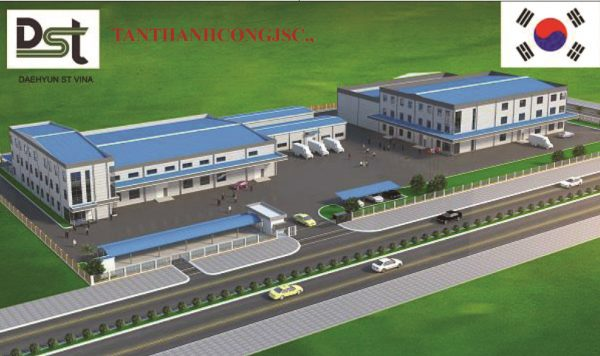
\includegraphics[height=41mm]{../../public/project-assets/daeyun.jpg}};
    \fill[TTCDeepNavy,opacity=.9] (63.5,132) rectangle (122.5,151);
  \end{scope}
  \draw[TTCBorder,rounded corners=3pt] (63.5,132) rectangle (122.5,190);
  \node[anchor=west,text=white,font=\fontsize{7.5}{8.8}\selectfont\bfseries] at (68.5,144) {ELECTRONIC \& CLEAN ROOM};
  \node[anchor=west,text=white!75!gray,font=\fontsize{5.8}{7}\selectfont] at (68.5,137) {HVAC • ESD • environmental control};

  \begin{scope}
    \clip[rounded corners=3pt] (127,132) rectangle (186,190);
    \node[inner sep=0pt] at (156.5,168) {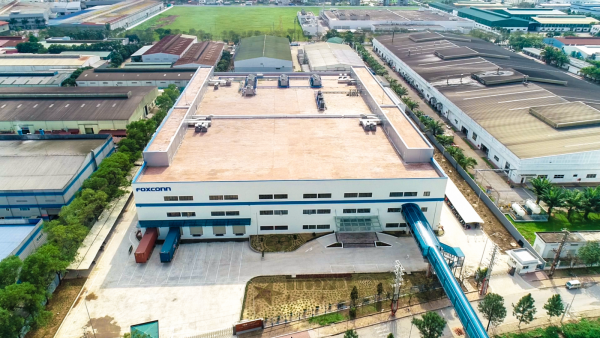
\includegraphics[height=41mm]{../../public/project-assets/foxcon.png}};
    \fill[TTCDeepNavy,opacity=.9] (127,132) rectangle (186,151);
  \end{scope}
  \draw[TTCBorder,rounded corners=3pt] (127,132) rectangle (186,190);
  \node[anchor=west,text=white,font=\fontsize{7.5}{8.8}\selectfont\bfseries] at (132,144) {ELECTRONIC FACTORY};
  \node[anchor=west,text=white!75!gray,font=\fontsize{5.8}{7}\selectfont] at (132,137) {MEP interface • erection by zone};

  % Hàng 2
  \begin{scope}
    \clip[rounded corners=3pt] (0,69) rectangle (59,127);
    \node[inner sep=0pt] at (29.5,103) {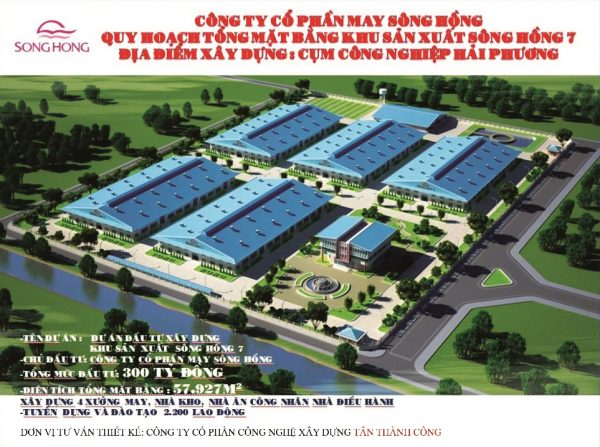
\includegraphics[height=42mm]{../../public/project-assets/songhong7.jpg}};
    \fill[TTCDeepNavy,opacity=.9] (0,69) rectangle (59,88);
  \end{scope}
  \draw[TTCBorder,rounded corners=3pt] (0,69) rectangle (59,127);
  \node[anchor=west,text=white,font=\fontsize{7.5}{8.8}\selectfont\bfseries] at (5,81) {MULTI-STOREY TEXTILES};
  \node[anchor=west,text=white!75!gray,font=\fontsize{5.8}{7}\selectfont] at (5,74) {Heavy loading floor • large span • escape};

  \begin{scope}
    \clip[rounded corners=3pt] (63.5,69) rectangle (122.5,127);
    \node[inner sep=0pt] at (93,104) {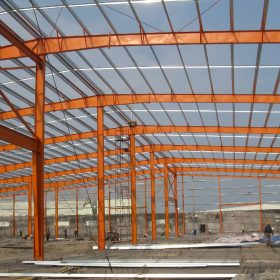
\includegraphics[width=60mm]{../../public/project-assets/yusen.jpg}};
    \fill[TTCDeepNavy,opacity=.9] (63.5,69) rectangle (122.5,88);
  \end{scope}
  \draw[TTCBorder,rounded corners=3pt] (63.5,69) rectangle (122.5,127);
  \node[anchor=west,text=white,font=\fontsize{7.5}{8.8}\selectfont\bfseries] at (68.5,81) {LOGISTICS \& LOGISTICS};
  \node[anchor=west,text=white!75!gray,font=\fontsize{5.8}{7}\selectfont] at (68.5,74) {Flat floor • dock • cargo flow};

  \begin{scope}
    \clip[rounded corners=3pt] (127,69) rectangle (186,127);
    \node[inner sep=0pt] at (156.5,104) {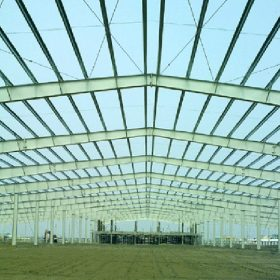
\includegraphics[width=60mm]{../../public/project-assets/sumidenso.jpg}};
    \fill[TTCDeepNavy,opacity=.9] (127,69) rectangle (186,88);
  \end{scope}
  \draw[TTCBorder,rounded corners=3pt] (127,69) rectangle (186,127);
  \node[anchor=west,text=white,font=\fontsize{7.5}{8.8}\selectfont\bfseries] at (132,81) {AUTO PARTS};
  \node[anchor=west,text=white!75!gray,font=\fontsize{5.8}{7}\selectfont] at (132,74) {Stable quality • handover according to gate};

  % Ba năng lực dùng chung
  \node[anchor=west,text=TTCBlue,font=\fontsize{8}{9.3}\selectfont\bfseries]
    at (0,58) {PROFILE ACROSS ALL INDUSTRY GROUPS};
  \foreach \xa/\xb/\title/\desc in {
    0/58/COORDINATION/architectural interface key • structure • MEP,
    64/122/CONSTRUCTABILITY/Design following construction methods and sequence,
    128/186/handover/Sufficient evidence before each transfer step}
  {
    \fill[TTCLightBlue,rounded corners=3pt] (\xa,20) rectangle (\xb,50);
    \node[anchor=west,text=TTCBlue,font=\fontsize{7.2}{8.5}\selectfont\bfseries]
      at ({\xa+6},41) {\title};
    \node[anchor=north west,text width=46mm,text=TTCTextMuted,
          font=\fontsize{6.1}{7.3}\selectfont] at ({\xa+6},34) {\desc};
  }
  \fill[TTCDeepNavy,rounded corners=3pt] (0,0) rectangle (186,12);
  \node[anchor=west,text=TTCCyan,font=\fontsize{6.2}{7.4}\selectfont\bfseries] at (7,6) {SECTOR FIT};
  \node[anchor=east,text=white,font=\fontsize{7}{8.3}\selectfont\bfseries]
    at (179,6) {TAILORED SOLUTION FOR OPERATIONAL NEEDS};
\end{tikzpicture}
\end{minipage}
\newpage

% ============================================================
% PAGE 30: BỘ HỒ SƠ BÀN GIAO
% ============================================================
\noindent\mbox{}\par\vspace{-\baselineskip}
\casepagebars{HANDOVER EVIDENCE • CLOSEOUT DOSSIER}{Page 30}

\begin{minipage}[t][246mm]{\textwidth}
\secbrand{Traceable Handover Dossier}{Evidence chain from approved material to as-built and commissioning records}

\noindent
\begin{tikzpicture}[x=1mm,y=1mm]
  \path[use as bounding box] (0,0) rectangle (186,220);
  \node[anchor=west,text=TTCBlue,font=\fontsize{15}{17}\selectfont\bfseries]
    at (0,211) {HANDOVER THE FACILITY — AND THE EVIDENCE};
  \node[anchor=west,text=TTCTextMuted,font=\fontsize{7.2}{8.8}\selectfont]
    at (0,201) {Each step is closed only when the technical documents, minutes and field evidence have matched.};

  % Dòng 5 cổng bằng chứng
  \fill[TTCLightBlue,rounded corners=4pt] (0,139) rectangle (186,190);
  \draw[TTCBorder,rounded corners=4pt] (0,139) rectangle (186,190);
  \draw[TTCBlue!40!white,line width=.8pt] (18,165) -- (168,165);
  \foreach \x/\n/\title in {
    1/18/MATERIALS,
    55.5/02/SHOP DRAWING,
    93/03/ACCEPTANCE TEST,
    130.5/04/AS-BUILT,
    168/05/COMMISSIONING}
  {
    \fill[white] (\x,165) circle (5mm);
    \draw[TTCBlue,line width=.8pt] (\x,165) circle (5mm);
    \node[text=TTCBlue,font=\fontsize{6}{7}\selectfont\bfseries] at (\x,165) {\n};
    \node[anchor=north,align=center,text width=29mm,text=TTCBlue,
          font=\fontsize{6.5}{7.7}\selectfont\bfseries] at (\x,155) {\title};
  }
  \fill[TTCRed] (18,165) circle (3.5mm);
  \node[text=white,font=\fontsize{5.8}{6.8}\selectfont\bfseries] at (18,165) {01};

  % Minh họa tập hồ sơ
  \fill[TTCDeepNavy,rounded corners=4pt] (0,48) rectangle (70,130);
  \node[anchor=west,text=TTCCyan,font=\fontsize{7}{8.2}\selectfont\bfseries]
    at (7,121) {CLOSEOUT DOSSIER};
  \fill[white!15!gray,rounded corners=2pt] (15,61) rectangle (61,111);
  \fill[white!45!gray,rounded corners=2pt] (12,65) rectangle (58,115);
  \fill[white,rounded corners=2pt] (9,69) rectangle (55,119);
  \fill[TTCRed] (9,112) rectangle (55,119);
  \node[anchor=west,text=TTCBlue,font=\fontsize{7.4}{8.6}\selectfont\bfseries]
    at (15,103) {AS-BUILT COMPANY};
  \draw[TTCBorder] (15,96) -- (49,96);
  \draw[TTCBorder] (15,90) -- (49,90);
  \draw[TTCBorder] (15,84) -- (42,84);
  \node[anchor=west,text=TTCTextMuted,font=\fontsize{5.8}{7}\selectfont]
    at (15,76) {CDE index • revision • approval};
  \node[anchor=west,text=white,font=\fontsize{6.1}{7.3}\selectfont\bfseries]
    at (7,55) {01 SET OF INDEXES • MULTIPLE GROUPS COMPANY};

  % Checklist bên phải
  \fill[white,rounded corners=4pt] (76,48) rectangle (186,130);
  \draw[TTCBorder,rounded corners=4pt] (76,48) rectangle (186,130);
  \node[anchor=west,text=TTCBlue,font=\fontsize{8}{9.4}\selectfont\bfseries]
    at (83,120) {MINIMUM HANDOVER STRUCTURE};
  \foreach \y/\n/\title/\desc in {
    104/01/COMPANY MATERIAL/Approved submittal • CO/CQ • MTC • test,
    90/02/COMPANY CONSTRUCTION/ITP • checklist • inspection and acceptance minutes,
    76/03/COMPANY AS-BUILT/As-built drawing • revision • confirmation,
    62/04/COMPANY OPERATING/O\&M manual • warranty • equipment list}
  {
    \fill[TTCLightBlue,rounded corners=2pt] (83,{\y-6}) rectangle (179,{\y+6});
    \node[anchor=west,text=TTCRed,font=\fontsize{6.2}{7.2}\selectfont\bfseries]
      at (88,\y) {\n};
    \node[anchor=west,text=TTCBlue,font=\fontsize{6.6}{7.7}\selectfont\bfseries]
      at (101,{\y+2}) {\title};
    \node[anchor=west,text=TTCTextMuted,font=\fontsize{5.6}{6.7}\selectfont]
      at (101,{\y-4}) {\desc};
  }

  % Nguyên tắc phát hành
  \node[anchor=west,text=TTCBlue,font=\fontsize{8}{9.3}\selectfont\bfseries]
    at (0,37) {ISSUANCE GUIDELINES};
  \fill[TTCDeepNavy,rounded corners=3pt] (0,0) rectangle (186,29);
  \node[anchor=west,text=TTCCyan,font=\fontsize{6.2}{7.4}\selectfont\bfseries]
    at (7,20) {RELEASE CONTROL};
  \node[anchor=west,text=white,font=\fontsize{9}{10.5}\selectfont\bfseries]
    at (7,10) {VERIFIED → SUFFICIENT APPROVED PROOF → OF → RETRIEVAL};
  \node[anchor=east,text=white!70!gray,font=\fontsize{6.1}{7.3}\selectfont]
    at (179,20) {An effective version • A handover index};
\end{tikzpicture}
\end{minipage}
\newpage

% ============================================================
% PAGE 31: NỀN TẢNG PHÁP LÝ VÀ HỆ QUẢN TRỊ
% ============================================================
\noindent\mbox{}\par\vspace{-\baselineskip}
\casepagebars{LEGAL FOUNDATION • GOVERNANCE SYSTEM}{Page 31}

\begin{minipage}[t][246mm]{\textwidth}
\secbrand{Due-Diligence-Ready Corporate Records}{Corporate identity • Construction capability • ISO systems • Key-person credentials}

\noindent
\begin{tikzpicture}[x=1mm,y=1mm]
  \path[use as bounding box] (0,0) rectangle (186,220);
  \node[anchor=west,text=TTCBlue,font=\fontsize{15}{17}\selectfont\bfseries]
    at (0,211) {ONE DOSSIER — FOUR VERIFIABLE CAPABILITY LAYERS};
  \node[anchor=west,text=TTCTextMuted,font=\fontsize{7.2}{8.8}\selectfont]
    at (0,201) {The legal entity information, scope of activities and management system are organized in accordance with the logic of the contractor appraisal round.};

  % Hồ sơ pháp nhân lớn bên trái
  \fill[TTCDeepNavy,rounded corners=4pt] (0,57) rectangle (67,191);
  \node[anchor=west,text=TTCCyan,font=\fontsize{7}{8.3}\selectfont\bfseries]
    at (7,182) {CORPORATE IDENTITY};
  \node[anchor=north west,text width=53mm,text=white,
        font=\fontsize{12}{14}\selectfont\bfseries]
    at (7,169) {JOINT STOCK COMPANY\\CONSTRUCTION TECHNOLOGY\\TAN THANH CONG};
  \draw[white!20!gray] (7,125) -- (60,125);
  \node[anchor=north west,text width=53mm,text=white!82!gray,
        font=\fontsize{6.5}{8.2}\selectfont]
    at (7,116) {\textbf{Abbreviated name:} TTC JSC\\[2mm]
                 \textbf{Tax code:} 0107090447\\[2mm]
                 \textbf{Headquarters:} Hanoi, Vietnam\\[2mm]
                 \textbf{Scope:} Industrial general contractor, steel structure, M\&E and project management};
  \fill[TTCRed,rounded corners=2pt] (7,67) rectangle (60,82);
  \node[text=white,font=\fontsize{7}{8.2}\selectfont\bfseries] at (33.5,74.5)
    {LEGAL • TRACEABLE • BID-READY};

  % Bốn lớp hồ sơ bên phải
  \foreach \y/\n/\title/\desc in {
    166/01/CONSTRUCTION CAPABILITY/The scope of work is directly reconciled according to the valid certificate; a copy is provided in the legal documents.,
    134/02/ISO MANAGEMENT SYSTEMS/ISO 9001 • ISO 14001 • ISO 45001 presented with the same scope of application and audit period.,
    102/03/KEY PERSONNEL/Practicing certificate of Project Manager • Site Manager • design lead.,
    70/04/COMPANY COMMERCIAL/Enterprise registration • tax • bank • insurance • bid form.}
  {
    \fill[white,rounded corners=3pt] (73,{\y-13}) rectangle (186,{\y+13});
    \draw[TTCBorder,rounded corners=3pt] (73,{\y-13}) rectangle (186,{\y+13});
    \fill[TTCLightBlue,rounded corners=2pt] (79,{\y-7}) rectangle (94,{\y+7});
    \node[text=TTCRed,font=\fontsize{7}{8}\selectfont\bfseries] at (86.5,\y) {\n};
    \node[anchor=west,text=TTCBlue,font=\fontsize{7.2}{8.5}\selectfont\bfseries]
      at (101,{\y+5}) {\title};
    \node[anchor=north west,text width=76mm,text=TTCTextMuted,
          font=\fontsize{6.1}{7.4}\selectfont] at (101,{\y-1}) {\desc};
  }

  % Checklist hồ sơ thầu
  \node[anchor=west,text=TTCBlue,font=\fontsize{8}{9.3}\selectfont\bfseries]
    at (0,46) {INDEX SET FOR PREQUALIFICATION /BIDDING};
  \foreach \xa/\xb/\label in {
    0/34/LEGAL ENTITY,
    38/72/PROFILE,
    76/110/ISO,
    114/148/HR,
    152/186/FINANCIAL}
  {
    \fill[TTCLightBlue,rounded corners=2pt] (\xa,20) rectangle (\xb,38);
    \node[text=TTCBlue,font=\fontsize{6.6}{7.8}\selectfont\bfseries]
      at ({(\xa+\xb)/2},29) {\label};
  }
  \fill[TTCDeepNavy,rounded corners=3pt] (0,0) rectangle (186,12);
  \node[anchor=west,text=TTCCyan,font=\fontsize{6.2}{7.4}\selectfont\bfseries] at (7,6) {DUE DILIGENCE};
  \node[anchor=east,text=white,font=\fontsize{7}{8.3}\selectfont\bfseries]
    at (179,6) {INDEXED INFORMATION • CONTROLLED COPY • EASY TO RECONCILE};
\end{tikzpicture}
\end{minipage}
\newpage

% ============================================================
% PAGE 32: BẢN ĐỒ HIỆN DIỆN DỰ ÁN
% ============================================================
\noindent\mbox{}\par\vspace{-\baselineskip}
\casepagebars{PROJECT FOOTPRINT • INDUSTRIAL CLUSTERS}{Page 32}

\begin{minipage}[t][246mm]{\textwidth}
\secbrand{Presence Along Vietnam's Key Industrial Corridors}{Northern manufacturing belt • Central corridor • Southern FDI and logistics cluster}

\noindent
\begin{tikzpicture}[x=1mm,y=1mm]
  \path[use as bounding box] (0,0) rectangle (186,220);
  \node[anchor=west,text=TTCBlue,font=\fontsize{15}{17}\selectfont\bfseries]
    at (0,211) {PROJECT DELIVERY EXPERIENCE ACROSS VIETNAM};
  \node[anchor=west,text=TTCTextMuted,font=\fontsize{7.2}{8.8}\selectfont]
    at (0,201) {Highlights reflect the cluster of areas appearing in the project list; do not represent the number of projects in proportion.};

  % Khung bản đồ
  \fill[white,rounded corners=4pt] (0,24) rectangle (103,191);
  \draw[TTCBorder,rounded corners=4pt,line width=.7pt] (0,24) rectangle (103,191);
  \node[inner sep=0pt] at (51.5,107.5)
    {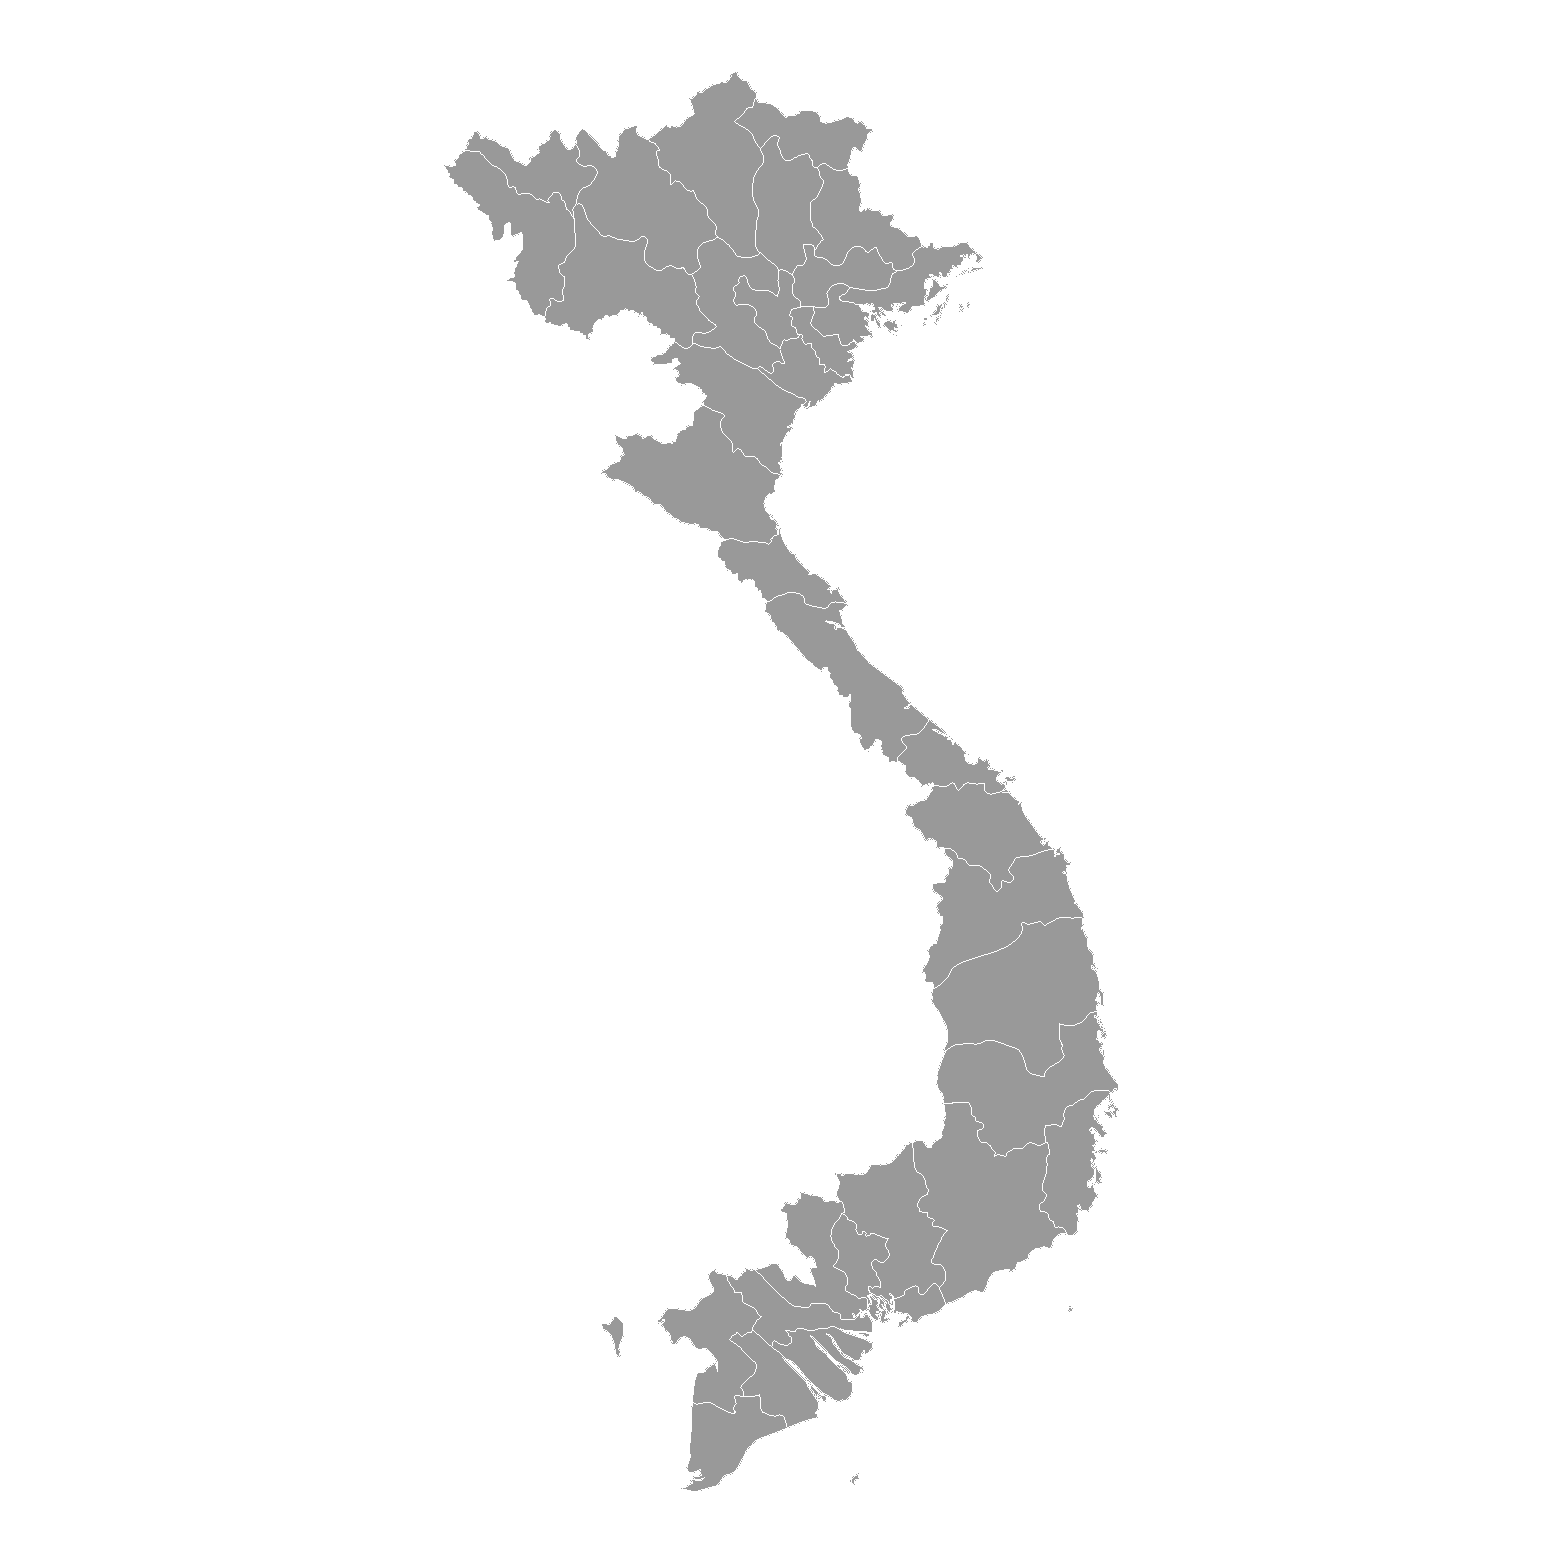
\includegraphics[height=164mm,trim=150 10 150 10,clip]{../../public/project-assets/vietnam-provinces.pdf}};

  % Highlight các cụm, vị trí chỉ báo gần đúng trên bản đồ nền
  \fill[TTCRed,opacity=.16] (62,151) circle (12mm);
  \draw[TTCRed,line width=1pt] (62,151) circle (6mm);
  \fill[TTCRed] (62,151) circle (2.2mm);
  \node[anchor=west,text=TTCRed,font=\fontsize{6.5}{7.6}\selectfont\bfseries] at (70,157) {NORTHERN CLUSTER};
  \node[anchor=west,text=TTCTextMuted,font=\fontsize{5.5}{6.6}\selectfont] at (70,150) {Hanoi • Vinh Phuc • Bac Ninh};

  \fill[TTCBlue,opacity=.14] (62,94) circle (10mm);
  \draw[TTCBlue,line width=1pt] (62,94) circle (5mm);
  \fill[TTCBlue] (62,94) circle (2mm);
  \node[anchor=west,text=TTCBlue,font=\fontsize{6.5}{7.6}\selectfont\bfseries] at (69,100) {CENTRAL CORRIDOR};
  \node[anchor=west,text=TTCTextMuted,font=\fontsize{5.5}{6.6}\selectfont] at (69,93) {Da Nang • Quang Nam • coastal};

  \fill[TTCCyan,opacity=.16] (51,51) circle (10mm);
  \draw[TTCCyan,line width=1pt] (51,51) circle (5mm);
  \fill[TTCCyan] (51,51) circle (2mm);
  \node[anchor=west,text=TTCBlue,font=\fontsize{6.5}{7.6}\selectfont\bfseries] at (59,57) {SOUTHERN CLUSTER};
  \node[anchor=west,text=TTCTextMuted,font=\fontsize{5.5}{6.6}\selectfont] at (59,50) {Binh Duong • HCMC • Hau Giang};
  \node[anchor=west,text=TTCTextMuted,font=\fontsize{4.8}{5.8}\selectfont]
    at (5,29) {CC0 background map: Wikimedia Commons / Thomson Walt};

  % Ba cụm thông tin bên phải
  \fill[TTCDeepNavy,rounded corners=4pt] (109,133) rectangle (186,191);
  \node[anchor=west,text=TTCCyan,font=\fontsize{6.2}{7.4}\selectfont\bfseries]
    at (116,183) {01 • CURRENT DEDICATION WEIGHT};
  \node[anchor=north west,text width=62mm,text=white,
        font=\fontsize{9.5}{11}\selectfont\bfseries] at (116,173) {NORTHERN INDUSTRIAL BELT};
  \node[anchor=north west,text width=62mm,text=white!75!gray,
        font=\fontsize{6.2}{7.6}\selectfont] at (116,153) {The project density is high around Hanoi, Vinh Phuc, Bac Ninh, Bac Giang, Hai Duong, Hai Phong and Nam Dinh industrial zones.};

  \fill[TTCLightBlue,rounded corners=4pt] (109,73) rectangle (186,127);
  \node[anchor=west,text=TTCRed,font=\fontsize{6.2}{7.4}\selectfont\bfseries]
    at (116,119) {02 • PROFILE MOBILE};
  \node[anchor=north west,text width=62mm,text=TTCBlue,
        font=\fontsize{8.5}{10}\selectfont\bfseries] at (116,109) {TEAM BY PROJECT CLUSTER};
  \node[anchor=north west,text width=62mm,text=TTCTextMuted,
        font=\fontsize{6.2}{7.6}\selectfont] at (116,92) {Arrange project management, QA/QC and HSE according to the area; the equipment mobilization plan is locked according to each work package.};

  \fill[white,rounded corners=4pt] (109,24) rectangle (186,67);
  \draw[TTCBorder,rounded corners=4pt] (109,24) rectangle (186,67);
  \node[anchor=west,text=TTCBlue,font=\fontsize{6.2}{7.4}\selectfont\bfseries]
    at (116,59) {03 • DIRECTION EXPAND};
  \node[anchor=north west,text width=62mm,text=TTCTextDark,
        font=\fontsize{6.3}{7.7}\selectfont] at (116,49) {Selective expansion in the Central and the South, prioritizing projects that require industrial EPC, logistics and high-tech factories.};

  \fill[TTCDeepNavy,rounded corners=3pt] (109,0) rectangle (186,16);
  \node[anchor=west,text=TTCCyan,font=\fontsize{6.1}{7.2}\selectfont\bfseries]
    at (116,8) {PROJECT FOOTPRINT};
  \node[anchor=east,text=white,font=\fontsize{6.5}{7.7}\selectfont\bfseries]
    at (179,8) {3 DEPLOYMENT CLUSTERS};
\end{tikzpicture}
\end{minipage}
\newpage

% ============================================================
% PAGE 33: LỘ TRÌNH 2026--2030
% ============================================================
\noindent\mbox{}\par\vspace{-\baselineskip}
\casepagebars{2026--2030 ROADMAP • CONTROLLED GROWTH}{Page 33}

\begin{minipage}[t][246mm]{\textwidth}
\secbrand{Selective \& Sustainable Development Roadmap}{Controlled development • Repeat clients • High-tech capability • Delivery discipline}

\noindent
\begin{tikzpicture}[x=1mm,y=1mm]
  \path[use as bounding box] (0,0) rectangle (186,220);
  \node[anchor=west,text=TTCBlue,font=\fontsize{15}{17}\selectfont\bfseries]
    at (0,211) {EXPAND ONLY WHEN GOVERNANCE IS READY};
  \node[anchor=west,text=TTCTextMuted,font=\fontsize{7.2}{8.8}\selectfont]
    at (0,201) {Prioritize delivery capability, repeat clients and governance quality before the pace of expansion.};

  % Ba horizon cards
  \foreach \xa/\xb/\year/\value/\focus/\desc in {
    0/58/2026/STANDARDIZATION/CONSOLIDATION OF PLATFORMS/General data environment • cost control • consolidation OF capacity IN the North,
    64/122/2027--2028/SELECTIVE/EXPAND CAPABILITY/High-Tech Projects • clean rooms • repeat customers,
    128/186/2029--2030/SUSTAINABLE/CONDITIONAL DEVELOPMENT/Controlled expansion • integrated capacity prioritization}
  {
    \fill[white,rounded corners=4pt] (\xa,68) rectangle (\xb,190);
    \draw[TTCBorder,rounded corners=4pt,line width=.7pt] (\xa,68) rectangle (\xb,190);
    \fill[TTCDeepNavy,rounded corners=4pt] (\xa,165) rectangle (\xb,190);
    \node[anchor=west,text=TTCCyan,font=\fontsize{7}{8.3}\selectfont\bfseries]
      at ({\xa+6},181) {\year};
    \node[anchor=west,text=white,font=\fontsize{13}{15}\selectfont\bfseries]
      at ({\xa+6},171) {\value};
    \fill[TTCRed] ({\xa+6},153) rectangle ({\xa+22},155);
    \node[anchor=west,text=TTCBlue,font=\fontsize{7.6}{9}\selectfont\bfseries]
      at ({\xa+6},143) {\focus};
    \node[anchor=north west,text width=46mm,text=TTCTextMuted,
          font=\fontsize{6.3}{7.7}\selectfont] at ({\xa+6},133) {\desc};
    \node[anchor=south west,text width=46mm,text=TTCTextDark,
          font=\fontsize{6.1}{7.5}\selectfont] at ({\xa+6},78)
      {\textbf{Step transition conditions:} key resources, contract risk, and handover's ability to meet the internal control threshold.};
  }

  % Các ưu tiên cụ thể để lấp đầy khoảng giữa và tăng khả năng ghi nhớ
  \foreach \y/\label in {116/Standardized data, 104/Base budget, 92/Northern capacity}{
    \fill[TTCRed] (6,\y) circle (1.2mm);
    \node[anchor=west,text=TTCTextDark,font=\fontsize{6.2}{7.4}\selectfont] at (11,\y) {\label};
  }
  \foreach \y/\label in {116/Clean room \& high-tech,104/Repeat clients,92/Multi-project governance}{
    \fill[TTCRed] (70,\y) circle (1.2mm);
    \node[anchor=west,text=TTCTextDark,font=\fontsize{6.2}{7.4}\selectfont] at (75,\y) {\label};
  }
  \foreach \y/\label in {116/Selected General Contractor ,104/Conditional Area ,92/Green Supply Chain}{
    \fill[TTCRed] (134,\y) circle (1.2mm);
    \node[anchor=west,text=TTCTextDark,font=\fontsize{6.2}{7.4}\selectfont] at (139,\y) {\label};
  }

  % Bốn bộ lọc tăng trưởng
  \node[anchor=west,text=TTCBlue,font=\fontsize{8}{9.3}\selectfont\bfseries]
    at (0,57) {FOUR FILTERS BEFORE SCALING};
  \foreach \xa/\xb/\n/\label in {
    0/43.5/01/SCOPE FIT,
    47.5/91/02/RESOURCES READY,
    95/138.5/03/CONTRACT RISK,
    142.5/186/04/HANDOVER CAPACITY}
  {
    \fill[TTCLightBlue,rounded corners=3pt] (\xa,25) rectangle (\xb,49);
    \node[anchor=west,text=TTCRed,font=\fontsize{6}{7}\selectfont\bfseries]
      at ({\xa+5},40) {\n};
    \node[anchor=west,text=TTCBlue,font=\fontsize{6.2}{7.4}\selectfont\bfseries]
      at ({\xa+5},32) {\label};
  }
  \node[anchor=west,text=TTCTextMuted,font=\fontsize{5.4}{6.5}\selectfont\itshape]
    at (0,14) {The roadmap is oriented; step by step expansion depends on capacity, market demand and governance approval.};
  \fill[TTCDeepNavy,rounded corners=3pt] (0,0) rectangle (186,10);
  \node[anchor=west,text=TTCCyan,font=\fontsize{6}{7.2}\selectfont\bfseries] at (7,5) {CONTROLLED GROWTH};
  \node[anchor=east,text=white,font=\fontsize{6.8}{8}\selectfont\bfseries]
    at (179,5) {HANDOVER QUALITY IS MORE IMPORTANT THAN SPEED};
\end{tikzpicture}
\end{minipage}
\newpage

% ============================================================
% PAGE 34: BẢO HÀNH VÀ HẬU MÃI
% ============================================================
\noindent\mbox{}\par\vspace{-\baselineskip}
\casepagebars{WARRANTY • AFTERCARE • OPERATIONAL SUPPORT}{Page 34}

\begin{minipage}[t][246mm]{\textwidth}
\secbrand{Single-Point Post-Handover Support}{Centralized intake • Contract-based response • Field verification • Closed-loop records}

\noindent
\begin{tikzpicture}[x=1mm,y=1mm]
  \path[use as bounding box] (0,0) rectangle (186,220);
  \node[anchor=west,text=TTCBlue,font=\fontsize{15}{17}\selectfont\bfseries]
    at (0,211) {HANDOVER IS NOT THE END};
  \node[anchor=west,text=TTCTextMuted,font=\fontsize{7.2}{8.8}\selectfont]
    at (0,201) {All requirements after handover are recorded, classified, processed and closed by the same chain of responsibility.};

  % Hero warranty promise
  \fill[TTCDeepNavy,rounded corners=4pt] (0,141) rectangle (54,190);
  \node[anchor=west,text=TTCCyan,font=\fontsize{6.4}{7.6}\selectfont\bfseries]
    at (7,181) {WARRANTY CONDITIONS};
  \node[anchor=center,align=center,text=white,font=\fontsize{18}{20}\selectfont\bfseries]
    at (27,163) {THEO\\CONTRACT};
  \node[anchor=center,align=center,text width=42mm,text=white!72!gray,font=\fontsize{5.5}{6.7}\selectfont]
    at (27,148) {Term and scope established in each contract};

  \fill[TTCLightBlue,rounded corners=4pt] (60,141) rectangle (186,190);
  \node[anchor=west,text=TTCBlue,font=\fontsize{8}{9.3}\selectfont\bfseries]
    at (67,181) {ONE CONTRACT RECEIVING — ONE COMPANY FOLLOWING};
  \node[anchor=north west,text width=104mm,text=TTCTextDark,
        font=\fontsize{6.7}{8.2}\selectfont] at (67,171)
    {Hotline and technical email are centralized reception channels. Response time, site inspection and remediation are determined according to priority, contractual conditions and access to the works.};
  \node[anchor=west,text=TTCRed,font=\fontsize{6.4}{7.6}\selectfont\bfseries]
    at (67,149) {NO PROFILE COMMITMENT • DO NOT CLOSE WITHOUT A CONFIRMATION};

  % Quy trình bốn bước
  \node[anchor=west,text=TTCBlue,font=\fontsize{8}{9.3}\selectfont\bfseries]
    at (0,130) {POST-HANDOVER SUPPORT PROCESS};
  \foreach \xa/\xb/\n/\title/\desc in {
    0/42/01/RECEIVE/record the phenomenon • image • degree of influence,
    48/90/02/CLASSIFICATION/Determination of warranty coverage and priority,
    96/138/03/INSPECTION/Remote assessment or site inspection arrangement,
    144/186/04/CLOSE COMPANY/Fix • inspection and acceptance • history update}
  {
    \fill[white,rounded corners=3pt] (\xa,78) rectangle (\xb,121);
    \draw[TTCBorder,rounded corners=3pt] (\xa,78) rectangle (\xb,121);
    \fill[TTCRed,rounded corners=1pt] ({\xa+5},109) rectangle ({\xa+16},118);
    \node[text=white,font=\fontsize{6}{7}\selectfont\bfseries] at ({\xa+10.5},113.5) {\n};
    \node[anchor=west,text=TTCBlue,font=\fontsize{7}{8.2}\selectfont\bfseries]
      at ({\xa+5},101) {\title};
    \node[anchor=north west,text width=31mm,text=TTCTextMuted,
          font=\fontsize{5.9}{7.2}\selectfont] at ({\xa+5},94) {\desc};
  }
  \foreach \xa/\xb in {42/48,90/96,138/144}{
    \draw[-{Latex[length=2mm]},TTCBlue!65!white,line width=.8pt]
      ({\xa+1},99) -- ({\xb-1},99);
  }

  % Phạm vi theo nhóm
  \node[anchor=west,text=TTCBlue,font=\fontsize{8}{9.3}\selectfont\bfseries]
    at (0,67) {THE SCOPE IS DETERMINED ACCORDING TO THE CONTRACT AND HANDOVER MINUTES};
  \foreach \xa/\xb/\title/\desc in {
    0/58/STRUCTURE/Frame • bonding • protective layer,
    64/122/COVER/Roof • wall • drainage • slot,
    128/186/M\&E \& Fire Protection/Equipment • system • operating records}
  {
    \fill[TTCLightBlue,rounded corners=3pt] (\xa,25) rectangle (\xb,58);
    \node[anchor=west,text=TTCBlue,font=\fontsize{7.2}{8.5}\selectfont\bfseries]
      at ({\xa+6},48) {\title};
    \node[anchor=north west,text width=46mm,text=TTCTextMuted,
          font=\fontsize{6}{7.3}\selectfont] at ({\xa+6},40) {\desc};
  }
  \fill[TTCDeepNavy,rounded corners=3pt] (0,0) rectangle (186,16);
  \node[anchor=west,text=TTCCyan,font=\fontsize{6.1}{7.3}\selectfont\bfseries] at (7,8) {CENTRAL SERVICE DESK};
  \node[anchor=east,text=white,font=\fontsize{6.8}{8}\selectfont\bfseries]
    at (179,8) {RECEIPT → OF → TRACE → CONFIRMATION PROCESSING};
\end{tikzpicture}
\end{minipage}
\newpage

% ============================================================
% PAGE 35: HỆ SINH THÁI ĐỐI TÁC — LOGO WALL
% ============================================================
\noindent\mbox{}\par\vspace{-\baselineskip}
\casepagebars{ECOSYSTEM • REFERENCES • COLLABORATION}{Page 35}

\begin{minipage}[t][246mm]{\textwidth}
\secbrand{Ecosystem \& Corporate References}{Selected corporate ecosystem and financial references}

\noindent
\begin{tikzpicture}[x=1mm,y=1mm]
  \path[use as bounding box] (0,0) rectangle (186,220);

  \node[anchor=west,text=TTCBlue,font=\fontsize{15}{17}\selectfont\bfseries]
    at (0,211) {CONNECTING CAPABILITIES • CREATING SHARED VALUE};
  \node[anchor=west,text width=178mm,text=TTCTextMuted,
        font=\fontsize{7.2}{8.8}\selectfont]
    at (0,199) {The brands are presented for ecosystem reference; the relationship and state of cooperation are collated according to the current profile.};

  % Nhóm doanh nghiệp: card lớn để giữ nhận diện của các logo dạng biểu tượng.
  \fill[TTCLightBlue,rounded corners=3pt] (0,177) rectangle (186,191);
  \node[anchor=west,text=TTCCyan,font=\fontsize{6.2}{7.4}\selectfont\bfseries]
    at (7,184) {CORPORATE ECOSYSTEM};
  \node[anchor=east,text=TTCBlue,font=\fontsize{7.2}{8.6}\selectfont\bfseries]
    at (179,184) {ENTERPRISE ECOSYSTEM};

  \newcommand{\corporatelogoclosing}[3]{%
    \fill[white,rounded corners=3pt] (#1,#2) rectangle ({#1+43.5},{#2+31});
    \draw[TTCBorder,rounded corners=3pt,line width=.6pt]
      (#1,#2) rectangle ({#1+43.5},{#2+31});
    \fill[TTCRed] ({#1+4},{#2+25.5}) rectangle ({#1+12},{#2+27});
    \node[inner sep=0pt] at ({#1+21.75},{#2+15})
      {\includegraphics[width=29mm,height=23mm,keepaspectratio]{#3}};
  }

  \corporatelogoclosing{0}{139}{../../public/logo/Food-logo.png}
  \corporatelogoclosing{47.5}{139}{../../public/logo/aidc_logo.png}
  \corporatelogoclosing{95}{139}{../../public/logo/alo-logo.png}
  \corporatelogoclosing{142.5}{139}{../../public/logo/company-minhphu.png}
  \corporatelogoclosing{0}{103}{../../public/logo/dieuphuong-logo.png}
  \corporatelogoclosing{47.5}{103}{../../public/logo/par5.png}
  \corporatelogoclosing{95}{103}{../../public/logo/y2y.png}
  \corporatelogoclosing{142.5}{103}{../../public/logo/company-sinchi.png}

  % Nhóm ngân hàng: 06 logo đúng với danh sách năng lực tín dụng trong hồ sơ.
  \fill[TTCLightBlue,rounded corners=3pt] (0,82) rectangle (186,96);
  \node[anchor=west,text=TTCCyan,font=\fontsize{6.2}{7.4}\selectfont\bfseries]
    at (7,89) {FINANCIAL REFERENCES};
  \node[anchor=east,text=TTCBlue,font=\fontsize{7.2}{8.6}\selectfont\bfseries]
    at (179,89) {REFERENCE FINANCIAL INSTITUTION};

  \newcommand{\banklogoclosing}[2]{%
    \fill[white,rounded corners=3pt] (#1,39) rectangle ({#1+28.5},75);
    \draw[TTCBorder,rounded corners=3pt,line width=.55pt]
      (#1,39) rectangle ({#1+28.5},75);
    \node[inner sep=0pt] at ({#1+14.25},57)
      {\includegraphics[width=23mm,height=17mm,keepaspectratio]{#2}};
  }
  \banklogoclosing{0}{../../public/logo/bank-acb.pdf}
  \banklogoclosing{31.5}{../../public/logo/bank-tpbank.pdf}
  \banklogoclosing{63}{../../public/logo/bank-vietcombank.pdf}
  \banklogoclosing{94.5}{../../public/logo/bank-bidv.pdf}
  \banklogoclosing{126}{../../public/logo/bank-vietinbank.png}
  \banklogoclosing{157.5}{../../public/logo/bank-mb.png}

  \fill[TTCDeepNavy,rounded corners=3pt] (0,0) rectangle (186,24);
  \fill[TTCRed,rounded corners=1pt] (7,7) rectangle (9,17);
  \node[anchor=west,text=white,font=\fontsize{8.4}{10}\selectfont\bfseries]
    at (15,15) {COLLABORATE FOR BETTER DELIVERY};
  \node[anchor=west,text=white!70!gray,font=\fontsize{6.1}{7.4}\selectfont]
    at (15,7) {Connect expertise, resources and financial capability to the project.};
  \node[anchor=east,text=TTCCyan,font=\fontsize{6.4}{7.6}\selectfont\bfseries]
    at (179,12) {PARTNERSHIP BUILT ON TRUST};
\end{tikzpicture}
\end{minipage}
\newpage

% ============================================================
% PAGE 36: BÌA SAU — NHẬN DIỆN THƯƠNG HIỆU
% ============================================================
\thispagestyle{empty}
\begin{tikzpicture}[remember picture,overlay]
  % Cùng hệ màu với bìa trước, không sử dụng ảnh.
  \fill[TTCDeepNavy] (current page.south west) rectangle (current page.north east);
  \fill[TTCRed] (current page.north west) rectangle ([yshift=-3mm]current page.north east);
  \fill[TTCRed] (current page.south west) rectangle ([yshift=3mm]current page.south east);

  % Hình học công nghiệp chìm tạo chiều sâu nhưng không cạnh tranh với nội dung.
  \begin{scope}[opacity=.075]
    \draw[white,line width=.8pt]
      ([xshift=16mm,yshift=122mm]current page.south west)
      -- ([xshift=16mm,yshift=146mm]current page.south west)
      -- ([xshift=52mm,yshift=168mm]current page.south west)
      -- ([xshift=88mm,yshift=146mm]current page.south west)
      -- ([xshift=124mm,yshift=178mm]current page.south west)
      -- ([xshift=158mm,yshift=146mm]current page.south west)
      -- ([xshift=194mm,yshift=166mm]current page.south west)
      -- ([xshift=194mm,yshift=122mm]current page.south west);
    \foreach \x in {28,40,64,76,100,112,136,148,172,184}{
      \draw[white,line width=.4pt]
        ([xshift=\x mm,yshift=122mm]current page.south west)
        -- ([xshift=\x mm,yshift=147mm]current page.south west);
    }
  \end{scope}
  \node[text=white,opacity=.025,font=\fontsize{92}{96}\selectfont\bfseries]
    at ([yshift=8mm]current page.center) {TTC};

  % Logo và nhận diện đầu trang.
  \node[anchor=north west,fill=white,rounded corners=4pt,
        inner xsep=7mm,inner ysep=4mm]
    at ([xshift=17mm,yshift=-20mm]current page.north west)
    {
\includegraphics[width=57mm]{../../public/logo-ttc-removebg-DNXrVdJp.png}};
  \node[anchor=north east,text=white!75!gray,font=\fontsize{6.5}{7.8}\selectfont\bfseries]
    at ([xshift=-17mm,yshift=-24mm]current page.north east) {COMPANY PROFILE • 2026};

  \node[anchor=north west,text=TTCCyan,font=\fontsize{7.5}{9}\selectfont\bfseries]
    at ([xshift=18mm,yshift=-78mm]current page.north west) {INDUSTRIAL DESIGN • BUILD • DELIVERY};
  \node[anchor=north west,text width=174mm,text=white,
        font=\fontsize{28}{31}\selectfont\bfseries]
    at ([xshift=18mm,yshift=-94mm]current page.north west)
    {BUILDING TOGETHER\\LASTING VALUE};
  \fill[TTCRed] ([xshift=18mm,yshift=-164mm]current page.north west)
    rectangle ([xshift=60mm,yshift=-167mm]current page.north west);
  \node[anchor=north west,text width=170mm,text=white!78!gray,
        font=\fontsize{8.2}{10.6}\selectfont]
    at ([xshift=18mm,yshift=-178mm]current page.north west)
    {Tan Thanh Cong is ready to accompany Client from concept, design to construction and handover industrial works.};

  % Khối thông tin sáng, rõ và nhận diện ngay khi lật tới bìa cuối.
  \fill[white,rounded corners=5pt]
    ([xshift=17mm,yshift=25mm]current page.south west)
    rectangle ([xshift=-17mm,yshift=104mm]current page.south east);
  \node[anchor=north west,text=TTCBlue,font=\fontsize{9.2}{11}\selectfont\bfseries]
    at ([xshift=26mm,yshift=94mm]current page.south west)
    {TAN THANH CONG TECHNOLOGY CONSTRUCTION JOINT STOCK COMPANY};
  \node[anchor=north west,text=TTCTextMuted,font=\fontsize{5.8}{7}\selectfont\bfseries]
    at ([xshift=26mm,yshift=83mm]current page.south west)
    {TAN THANH CONG TECHNOLOGY CONSTRUCTION JOINT STOCK COMPANY};
  \draw[TTCBorder,line width=.6pt]
    ([xshift=26mm,yshift=75mm]current page.south west)
    -- ([xshift=-26mm,yshift=75mm]current page.south east);

  \node[anchor=north west,text width=148mm,text=TTCTextDark,
        font=\fontsize{7}{9.2}\selectfont]
    at ([xshift=26mm,yshift=69mm]current page.south west)
    {\textcolor{TTCRed}{\faMapMarker*}\quad
     \textbf{Registered office:} No. 39, Lane 292 Kim Giang, Dai Kim, Hanoi\\[2.3mm]
     \textcolor{TTCRed}{\faBuilding}\quad
     \textbf{Trading office:} No. 19N7B, Urban area Trung Hoa Nhan Chinh, Hanoi\\[2.3mm]
     \textcolor{TTCRed}{\faPhone*}\quad 0976 447 766
     \hspace{12mm}\textcolor{TTCRed}{\faEnvelope}\quad info@tanthanhcongjsc.com
     \hspace{12mm}\textcolor{TTCRed}{\faGlobe}\quad tanthanhcongjsc.com};

  \node[anchor=south west,text=white!65!gray,font=\fontsize{5.6}{6.8}\selectfont]
    at ([xshift=17mm,yshift=8mm]current page.south west)
    {\textcopyright\ 2026 TAN THANH CONG JSC};
  \node[anchor=south east,text=TTCCyan,font=\fontsize{6.2}{7.4}\selectfont\bfseries]
    at ([xshift=-17mm,yshift=8mm]current page.south east)
    {TANTHANHCONGJSC.COM};
\end{tikzpicture}


\end{document}
